\begingroup
\renewcommand{\arraystretch}{0.8}%
\setlength{\tabcolsep}{0.3pt}
\begin{figure}[p]
\setkeys{Gin}{width=\linewidth}
\Huge
\begin{tabularx}{\textwidth}{CCCC}
\multicolumn{4}{p{\linewidth}}{\large \centering \textbf{\emph{P. luminescens} TT01 PVC ``Unit 1"}} \\
\hiderowcolors
& & & \\[-1.5ex]
\Large 2 Hours &\Large 5 Hours &\Large 24 Hours &\Large 72 Hours \\[1ex]

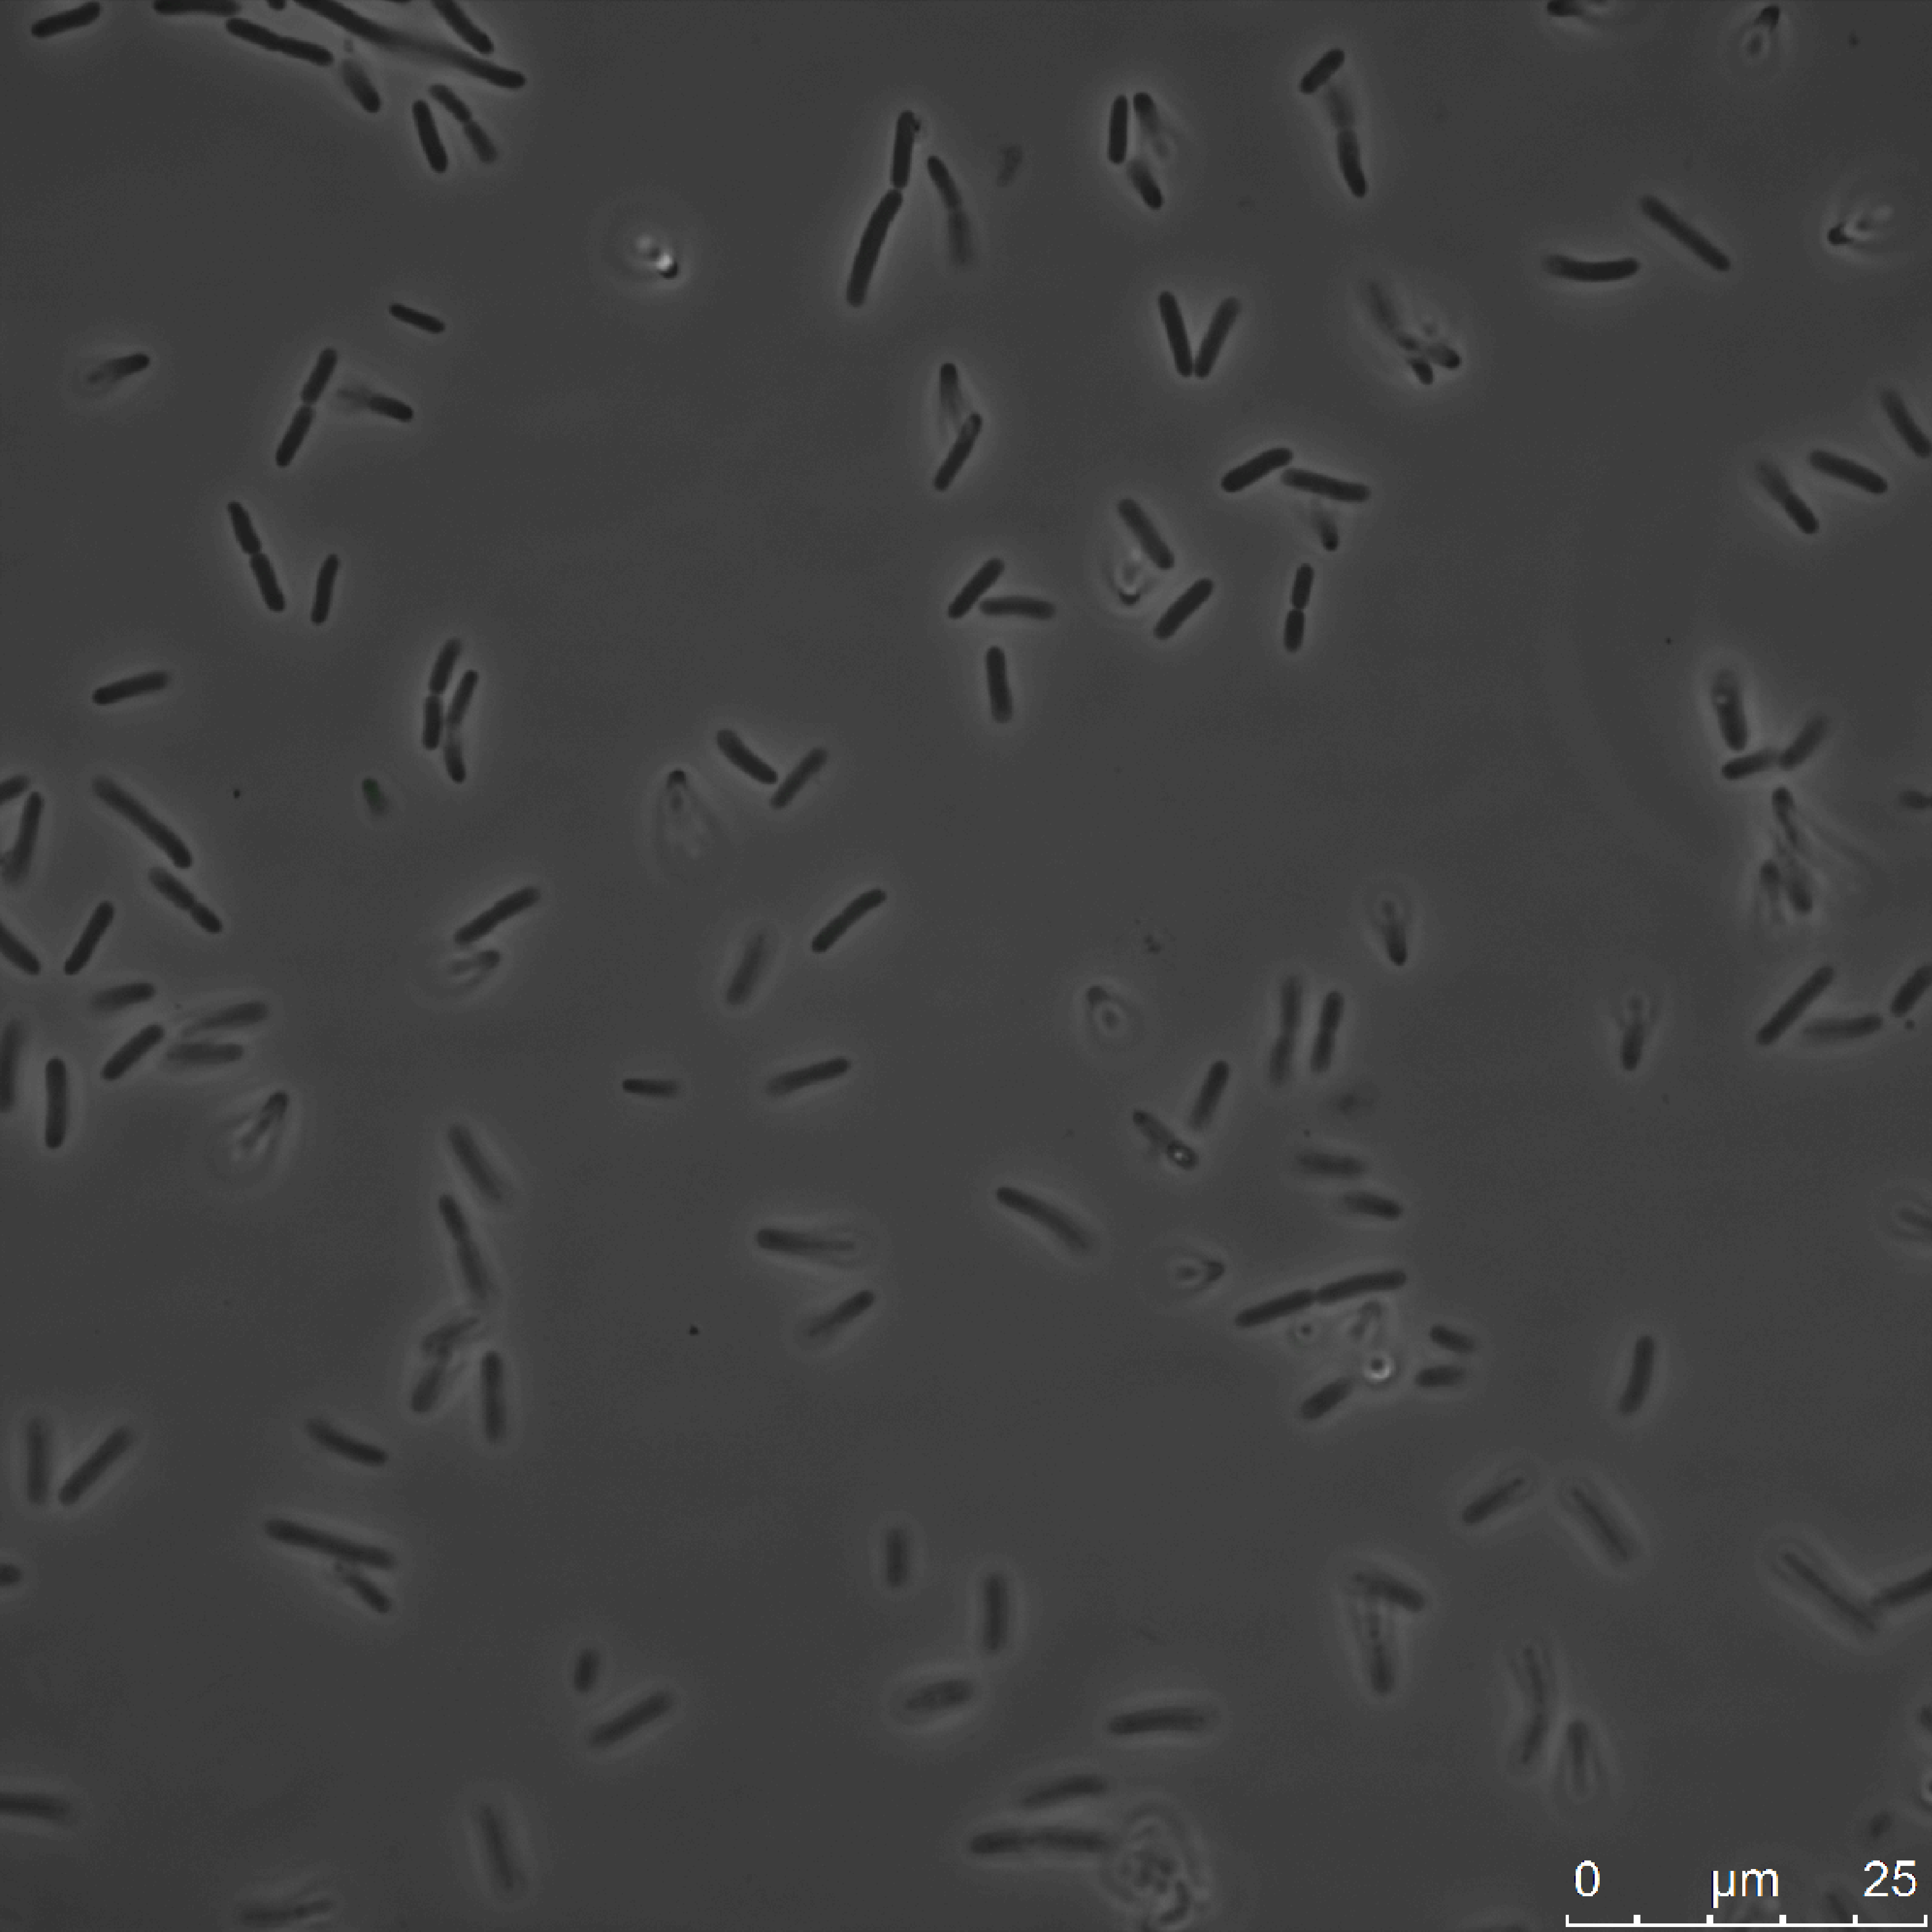
\includegraphics{TT01U1_1_NOGREEN.pdf} &%
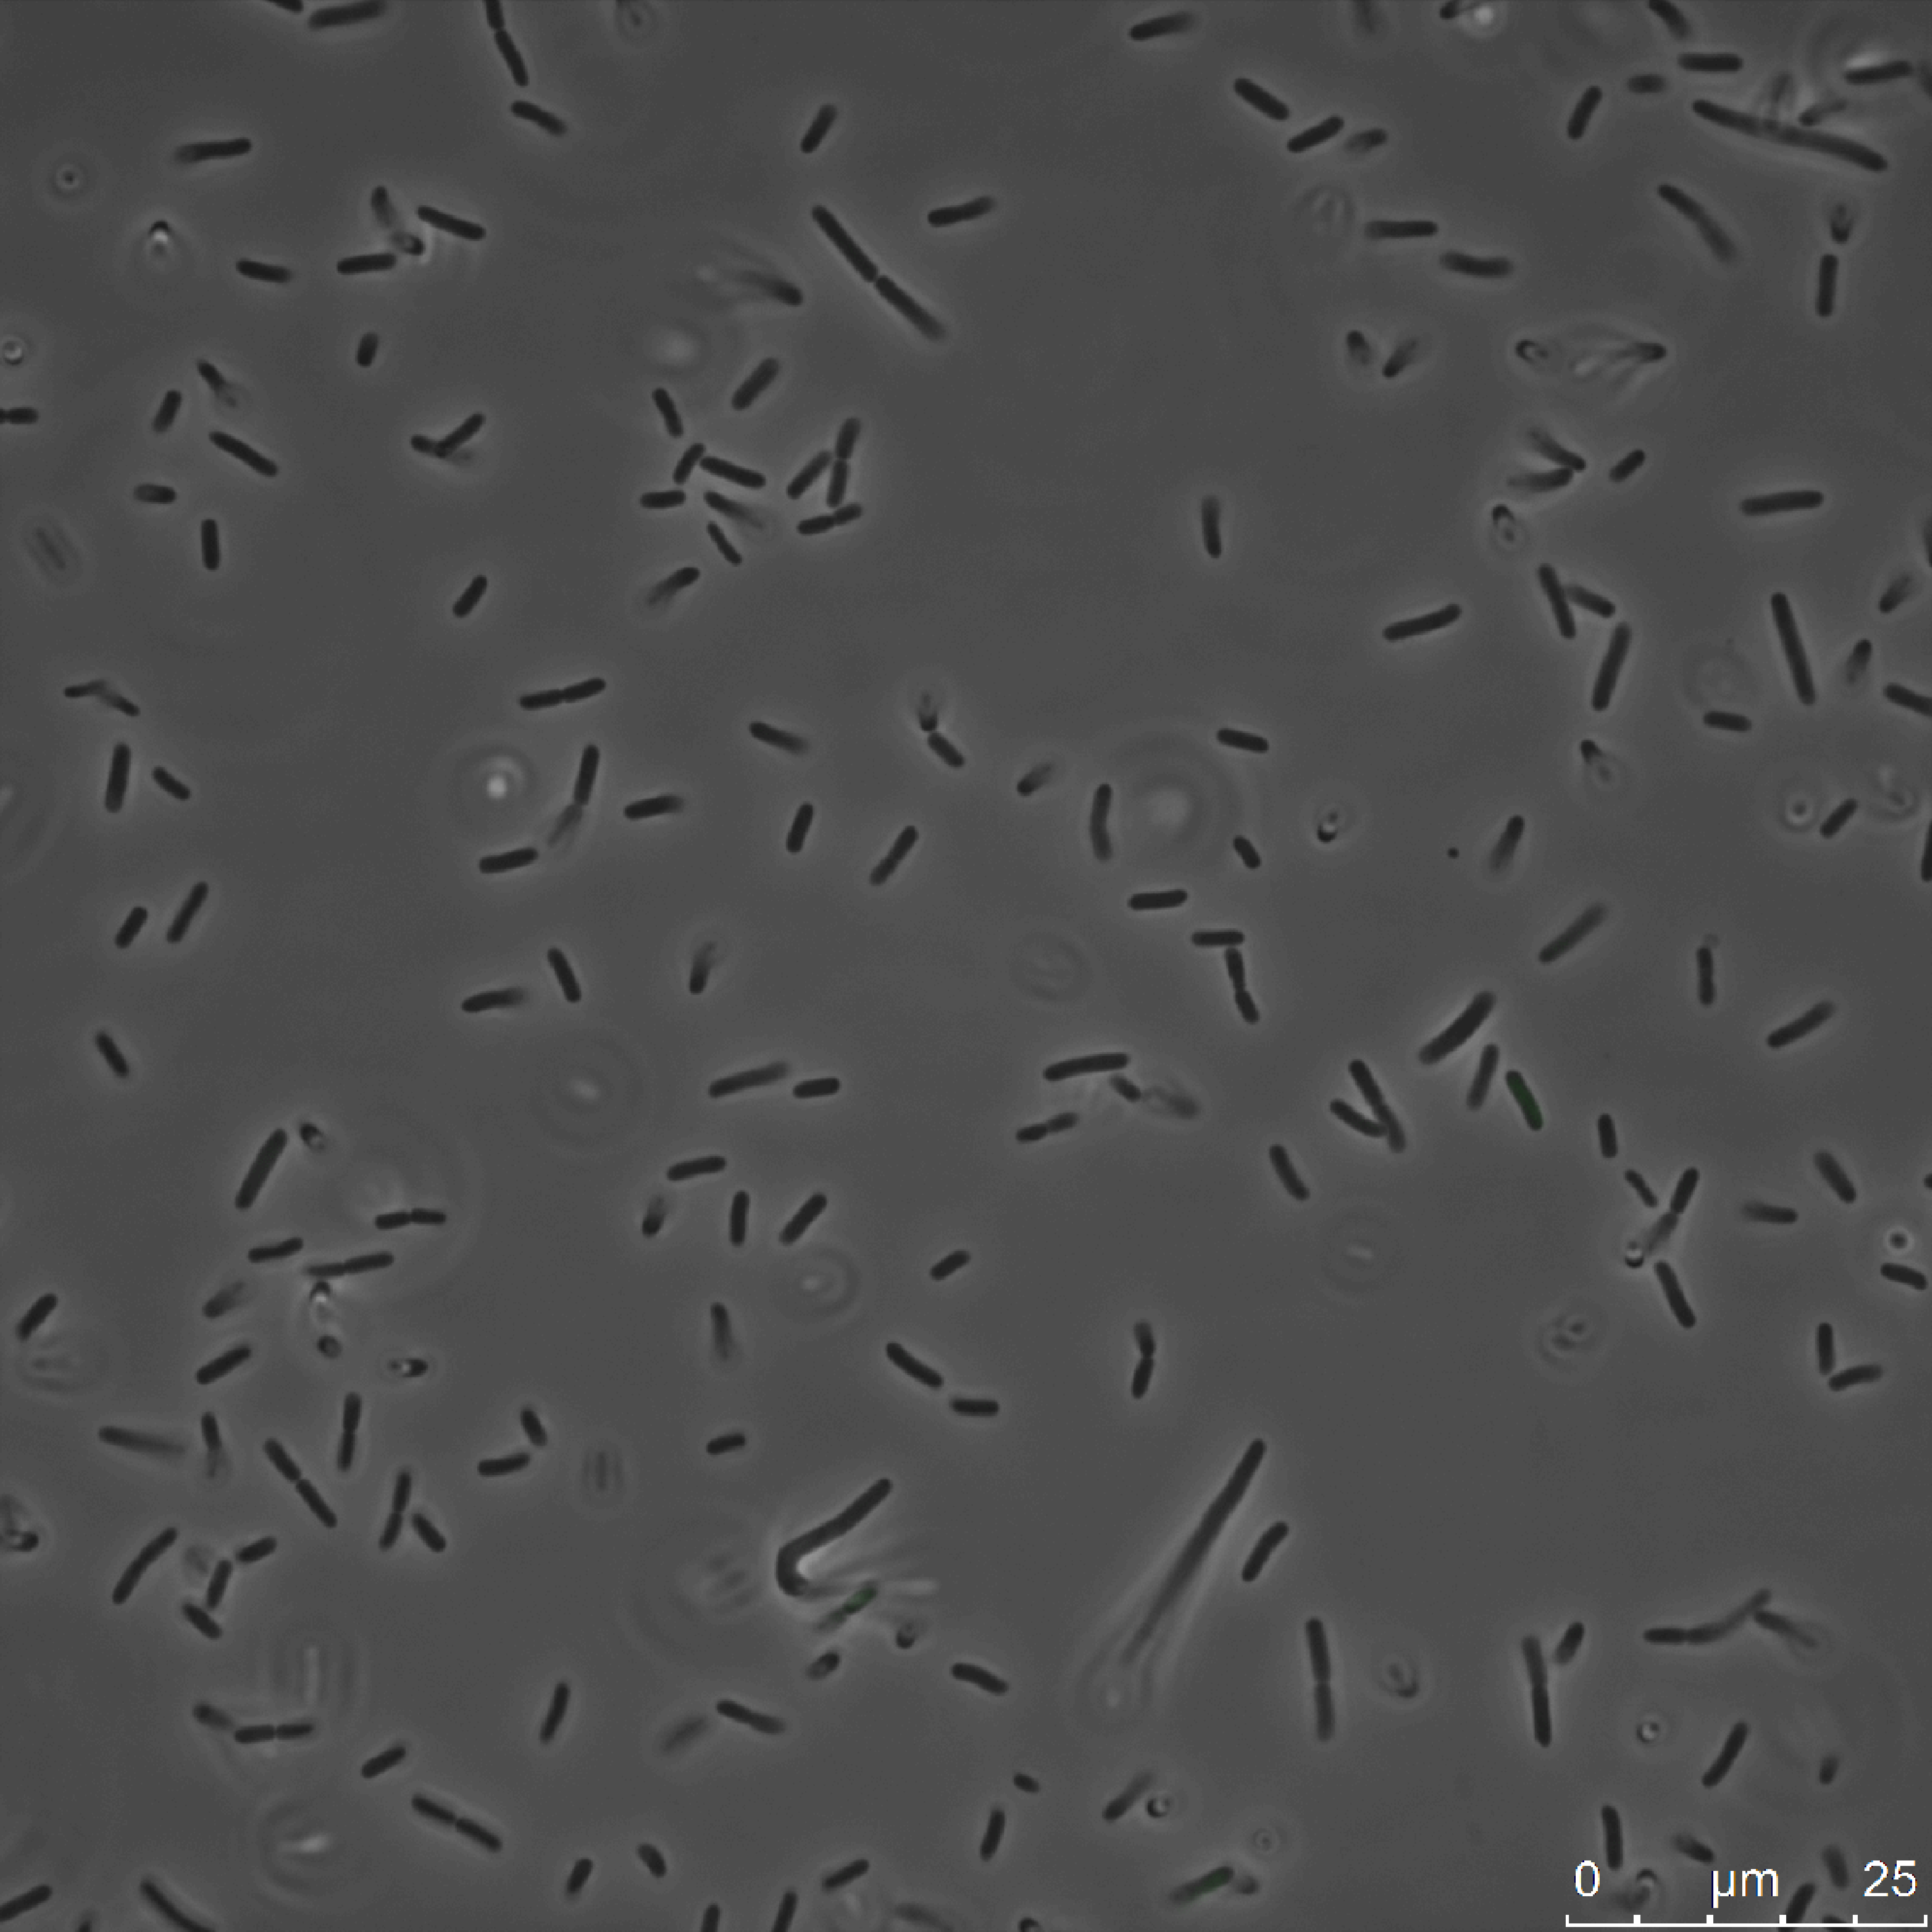
\includegraphics{TT01U1_5HR_5_LOWGREEN.pdf} &%
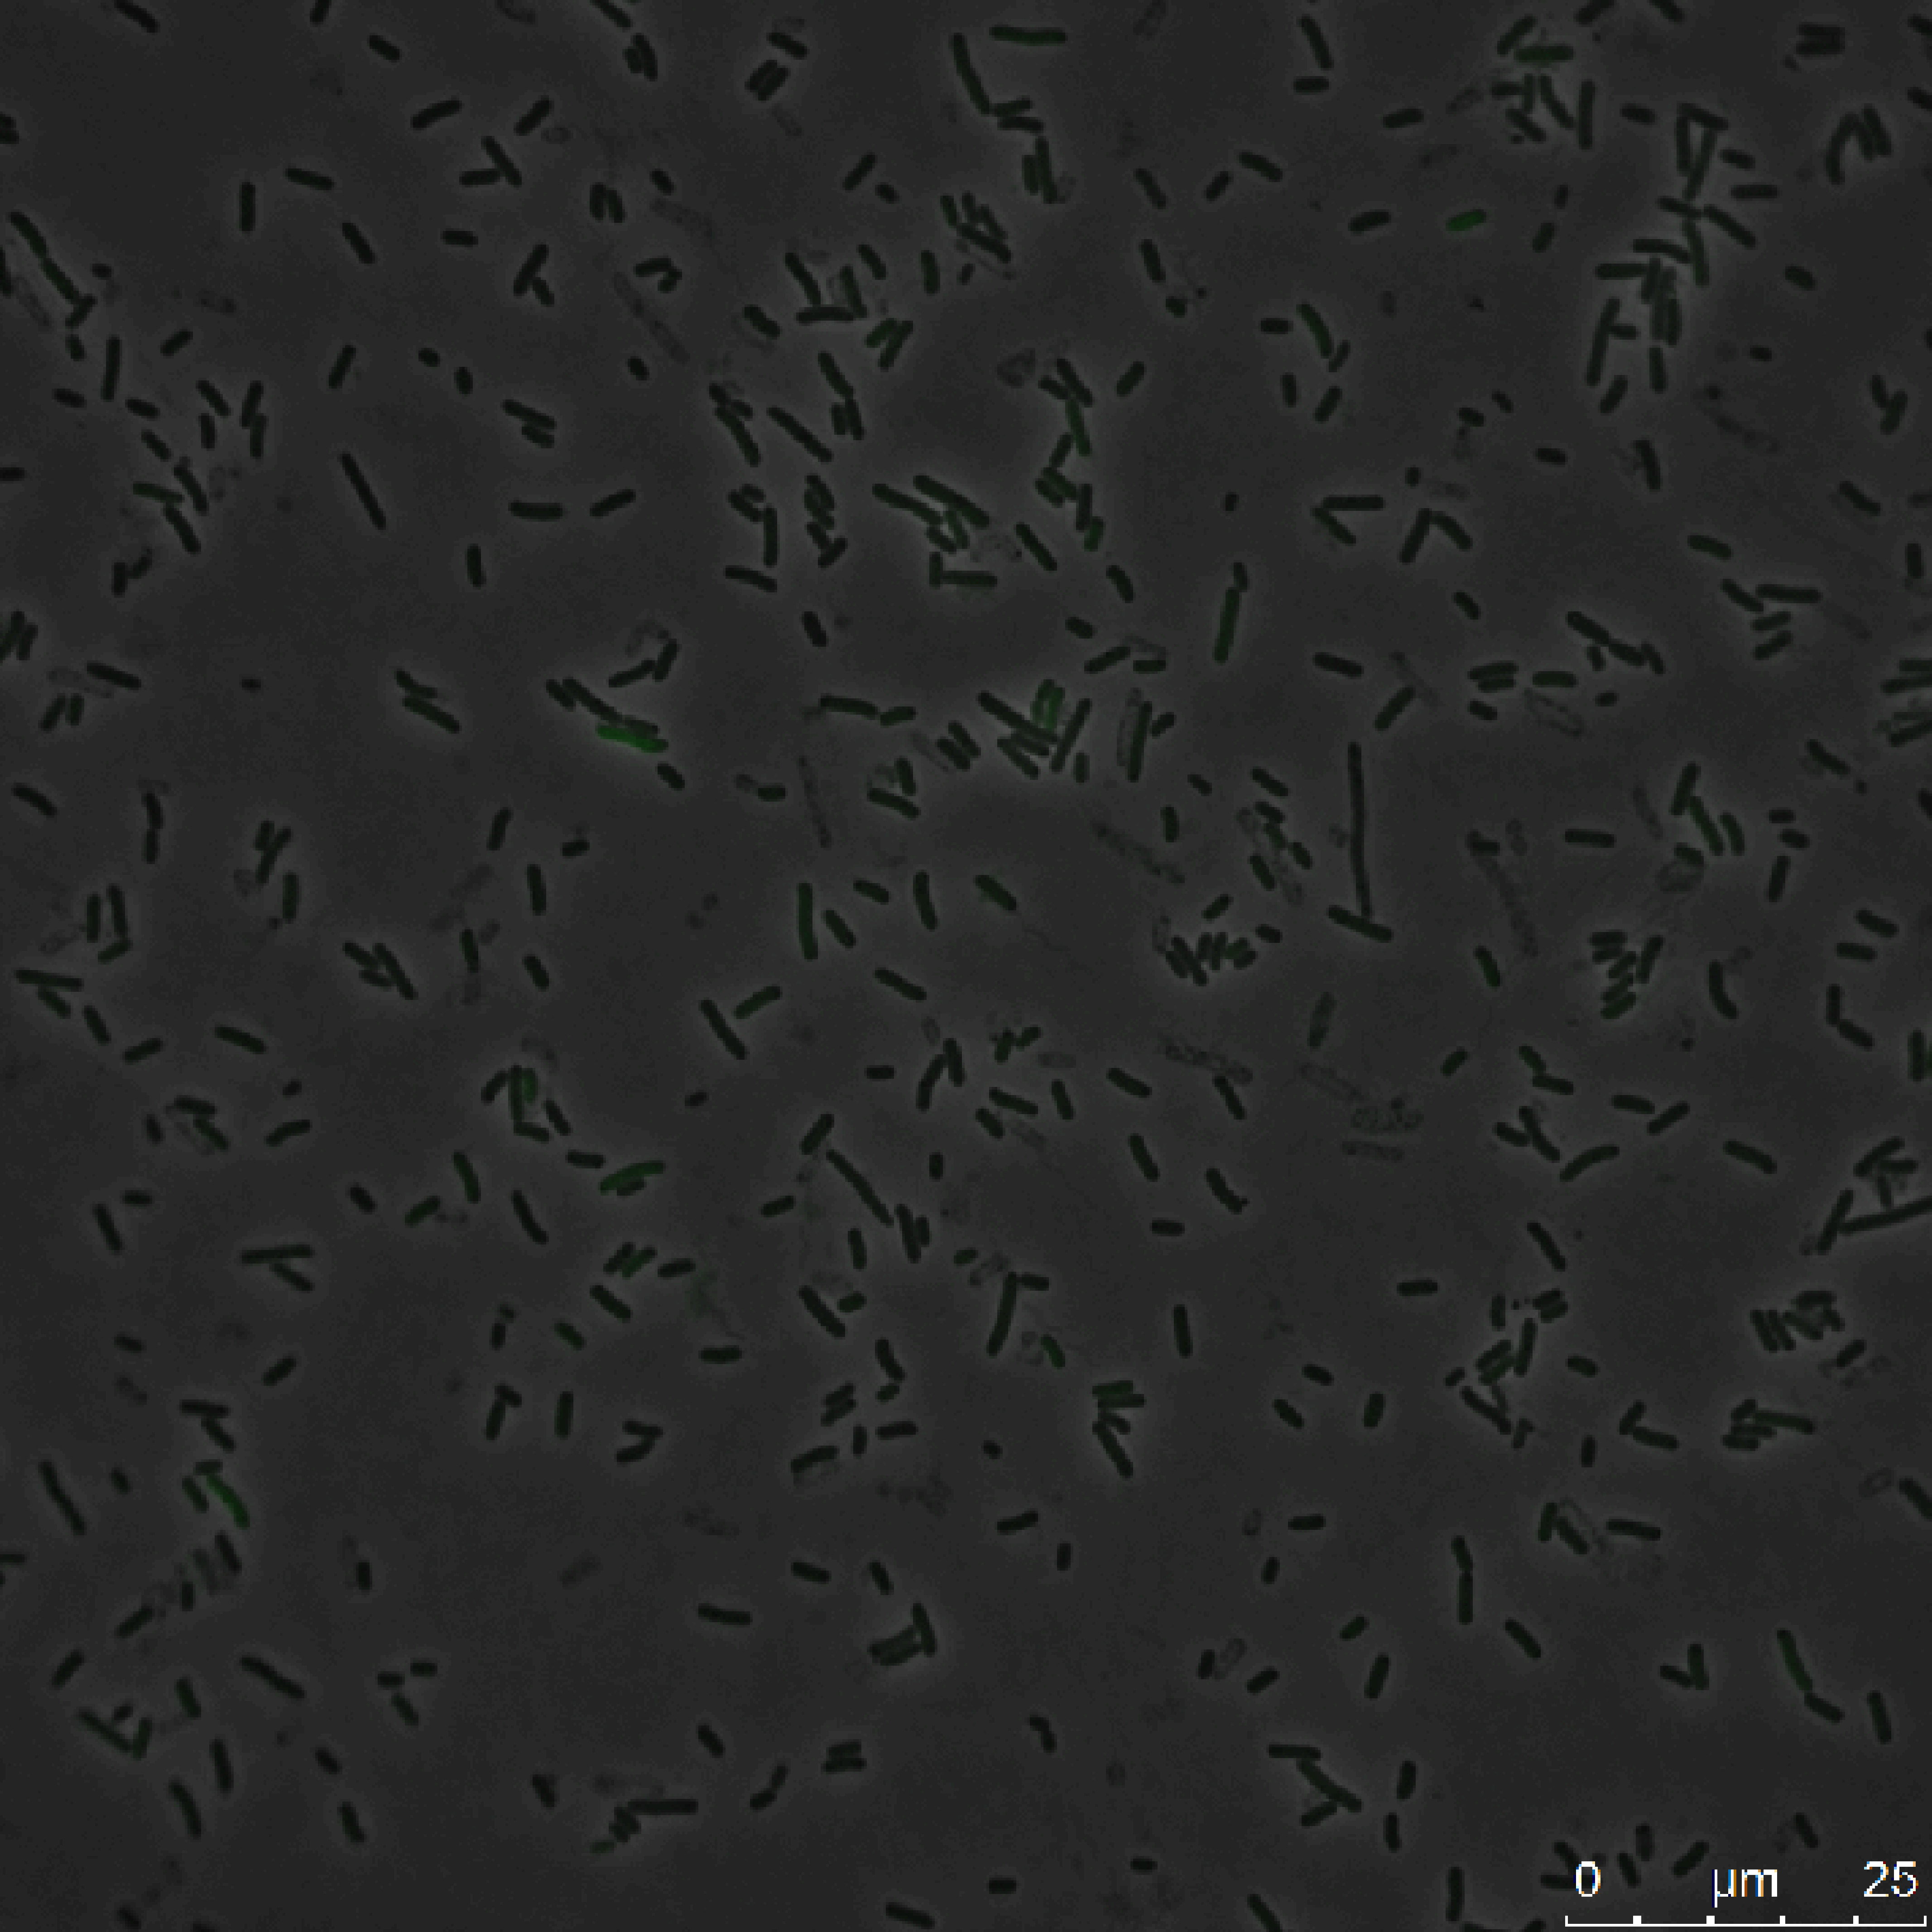
\includegraphics{TT01U1_24HR_1_GREEN.pdf} &%
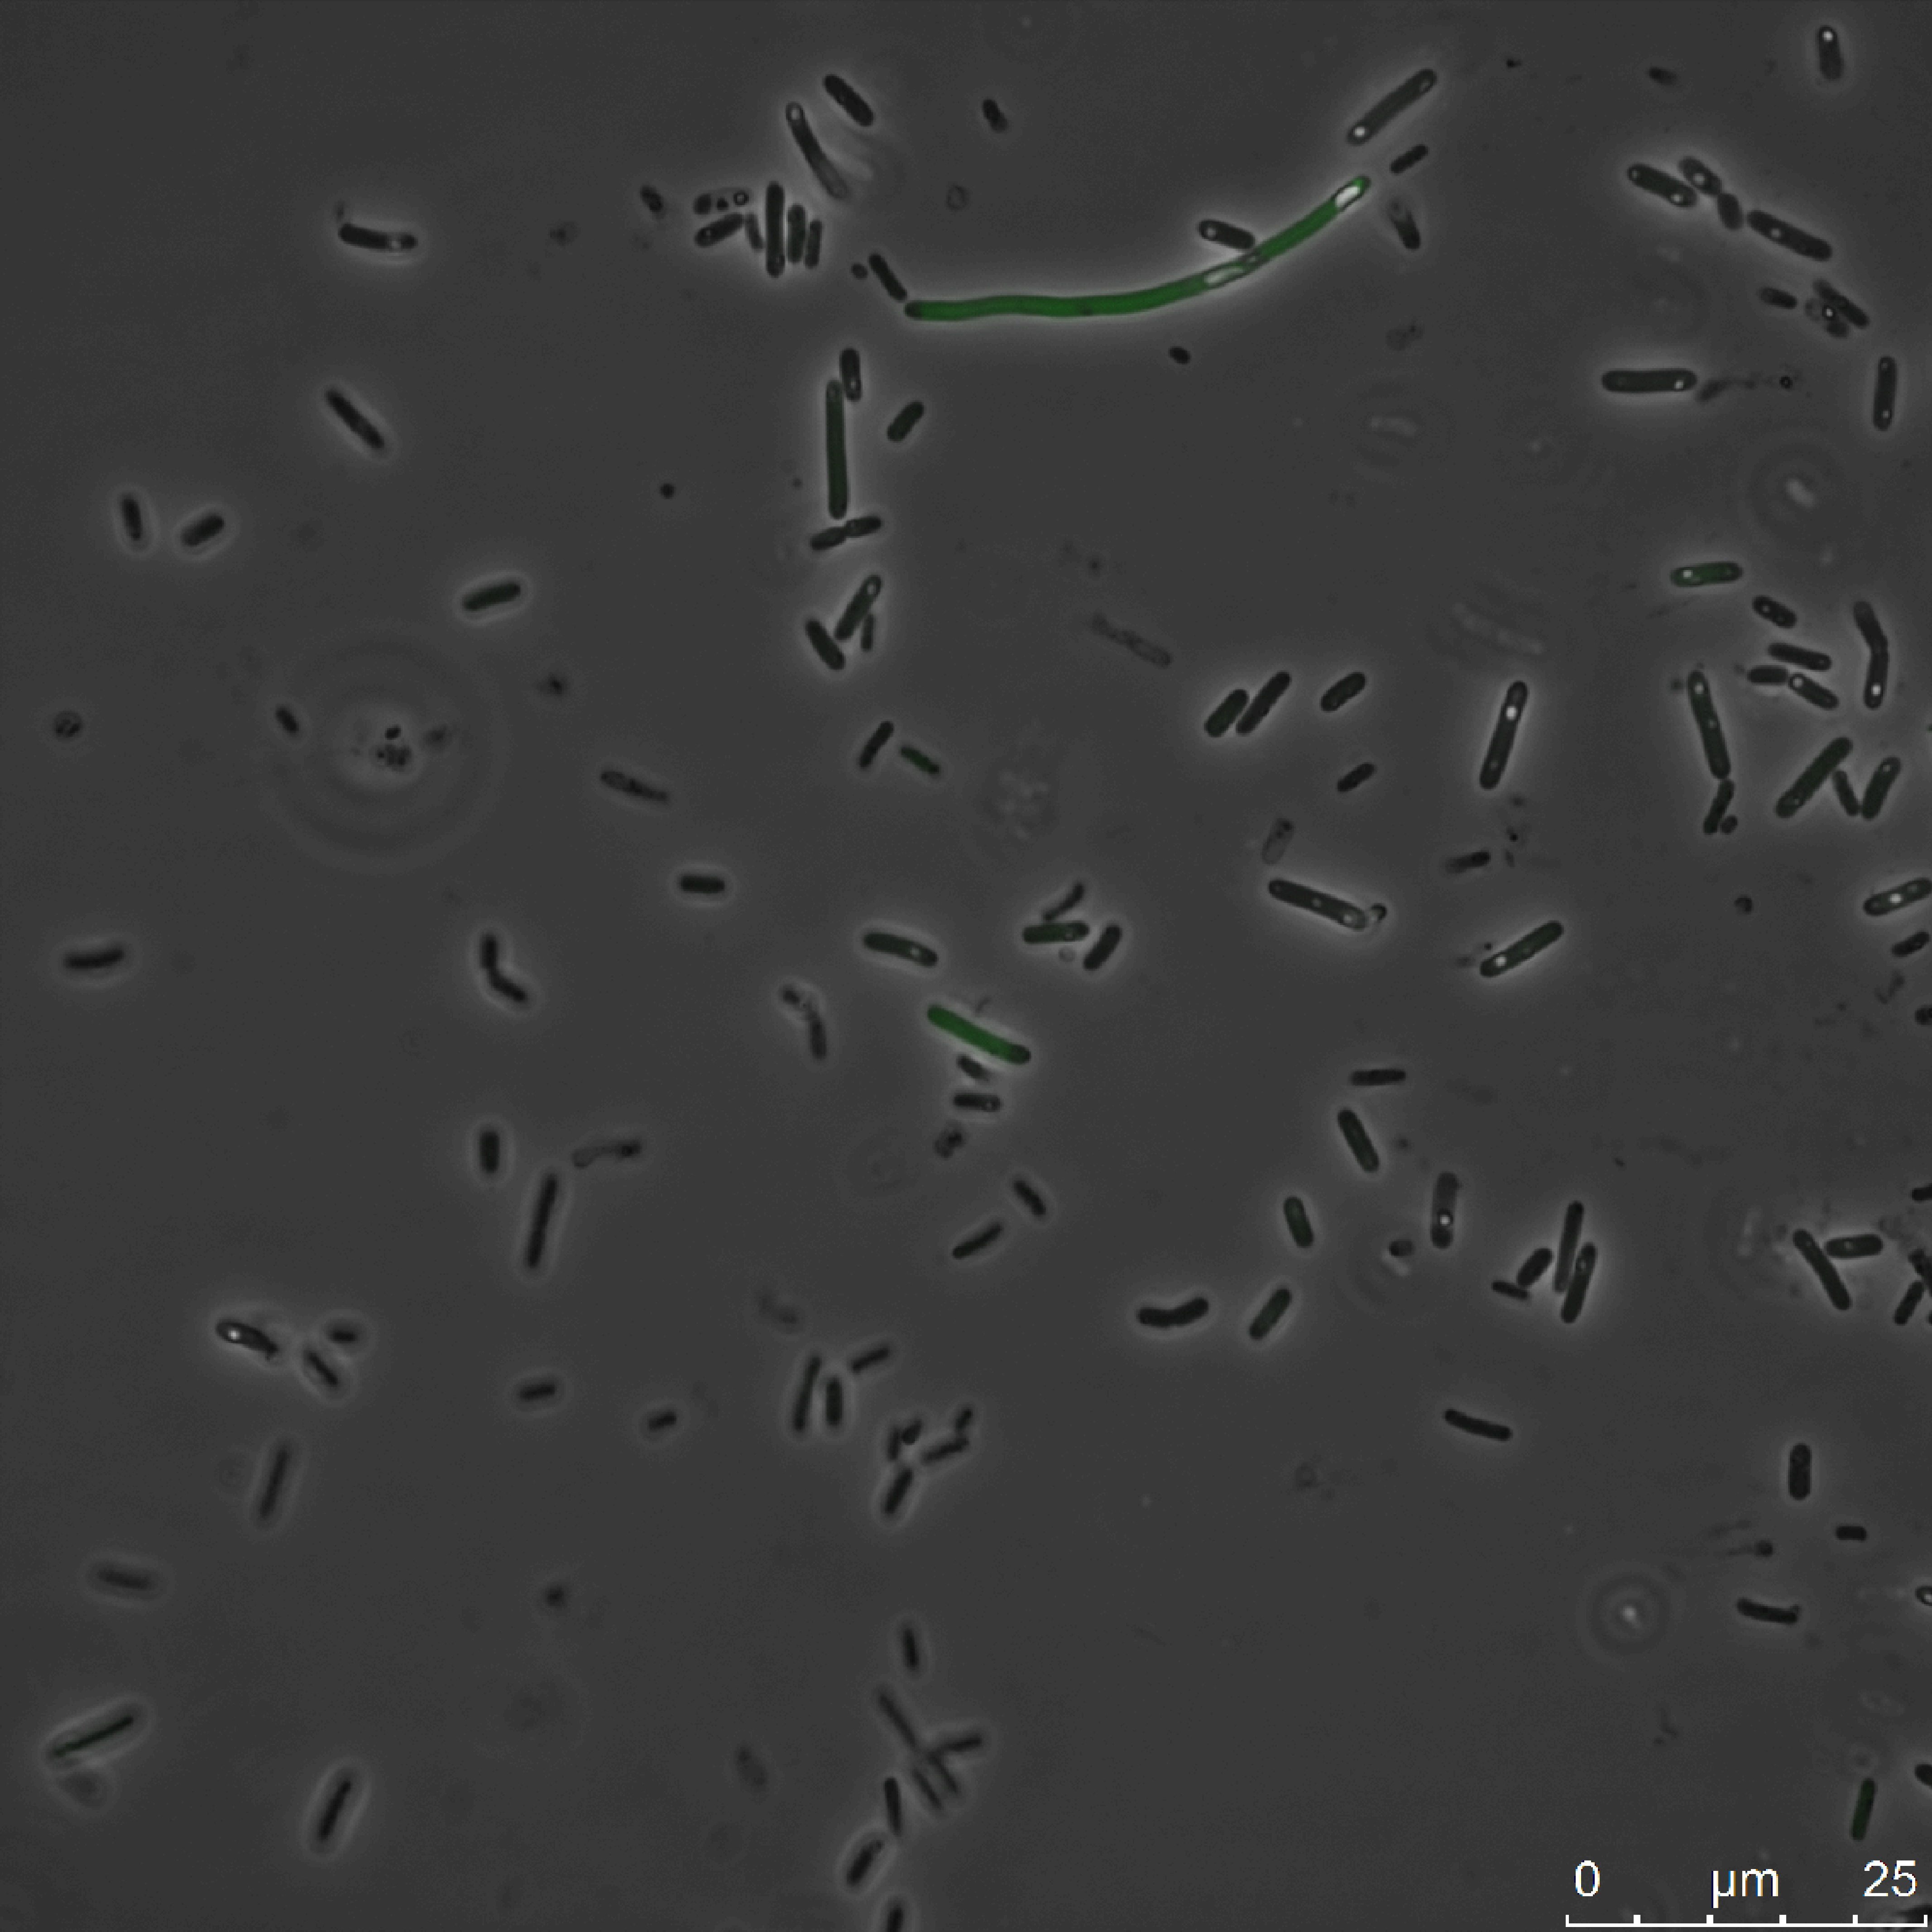
\includegraphics{TT01U1_72HR_1_GREEN.pdf} \\[-0.5ex]

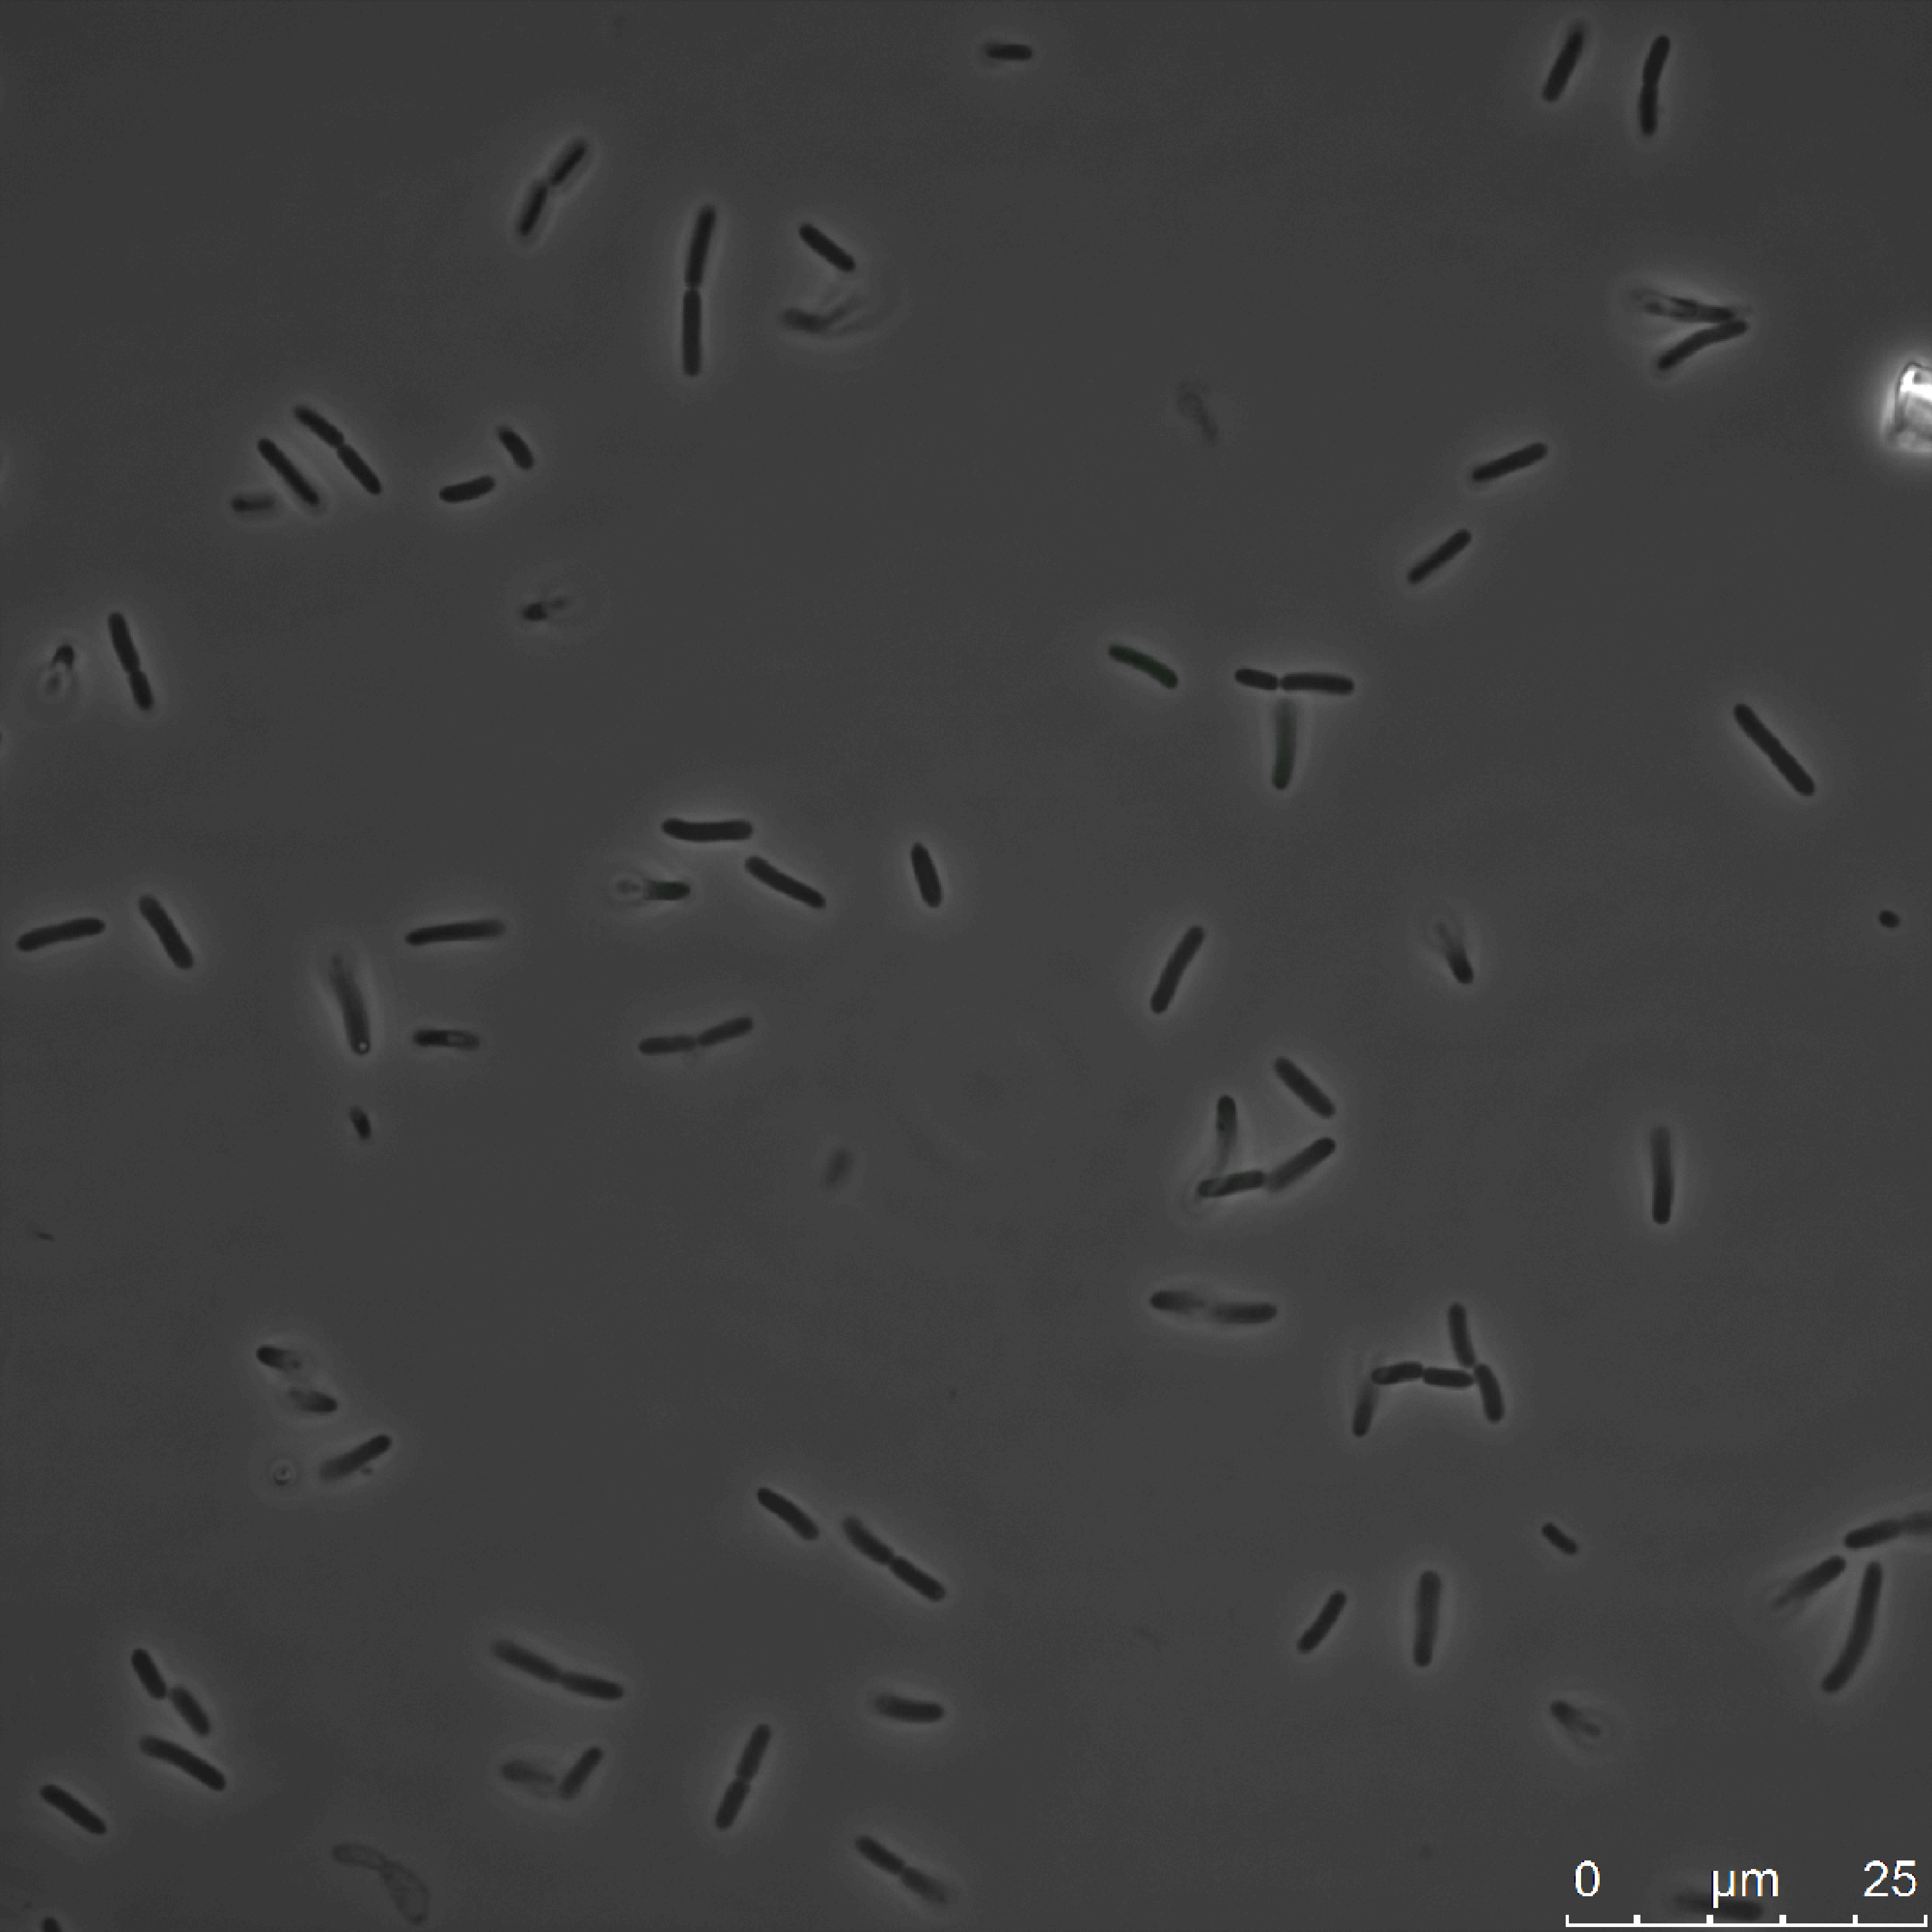
\includegraphics{TT01U1_2_NOGREEN.pdf} &%
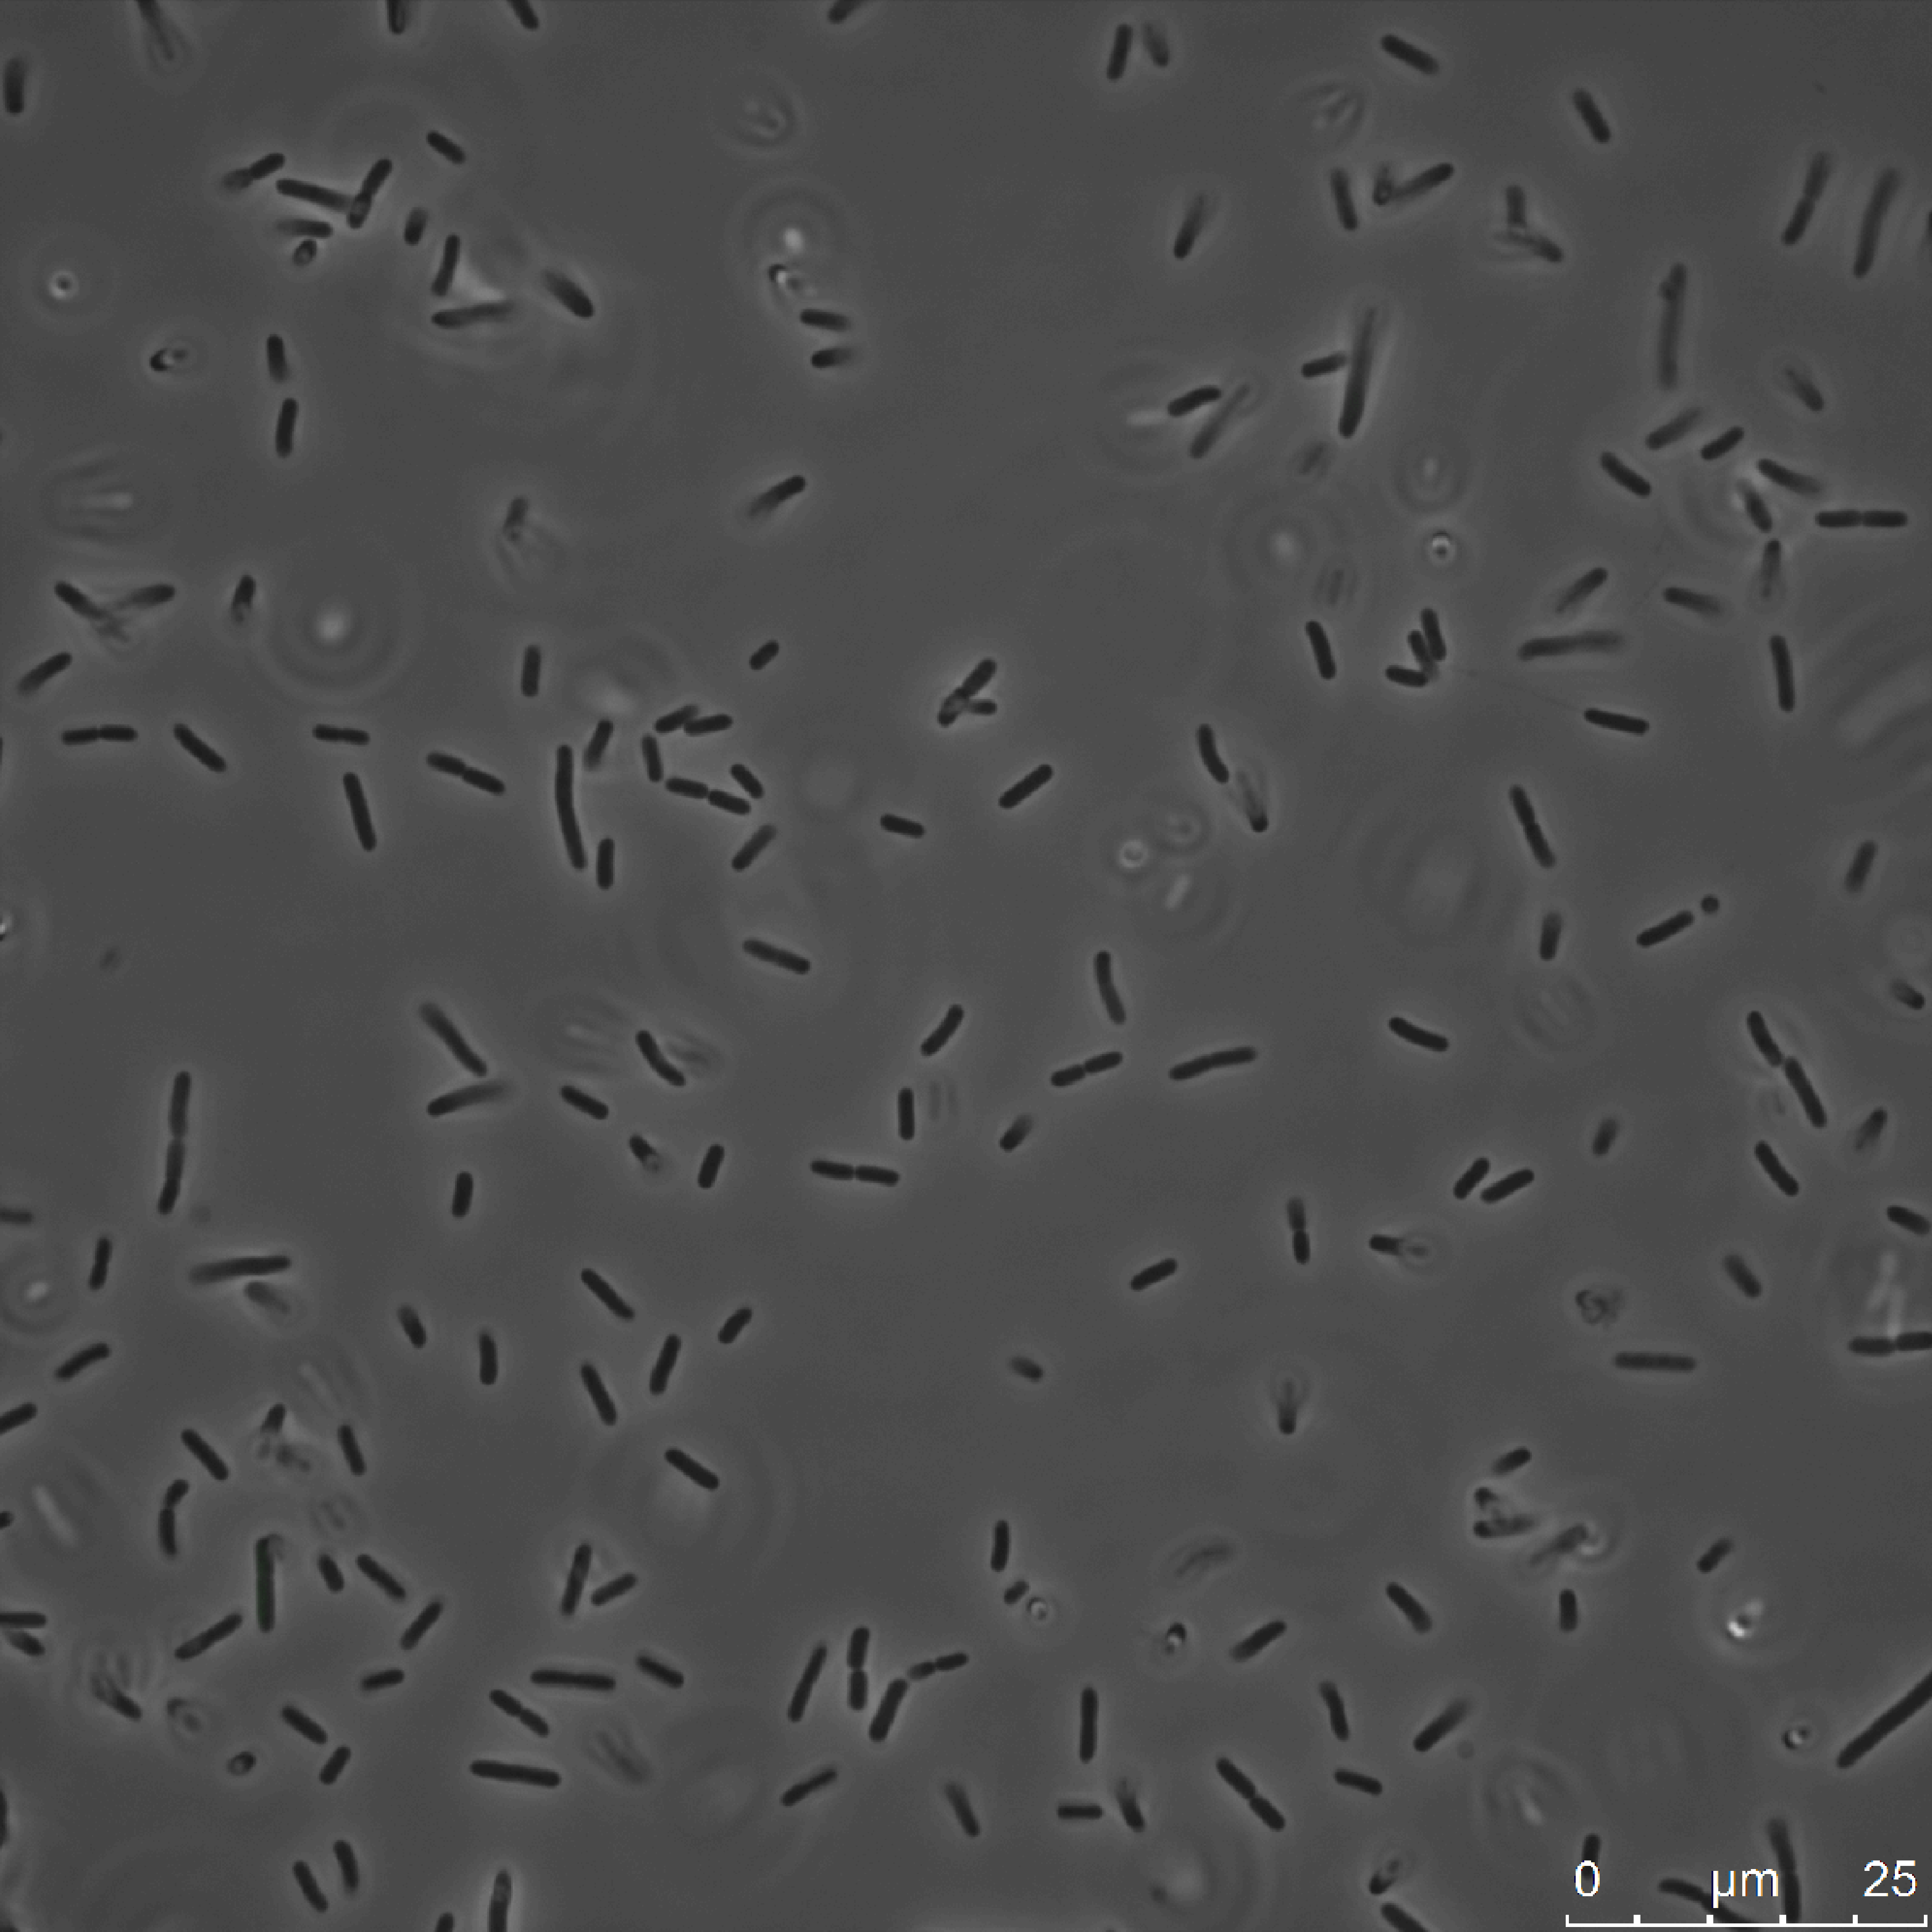
\includegraphics{TT01U1_5HR_2_NOGREEN.pdf} &%
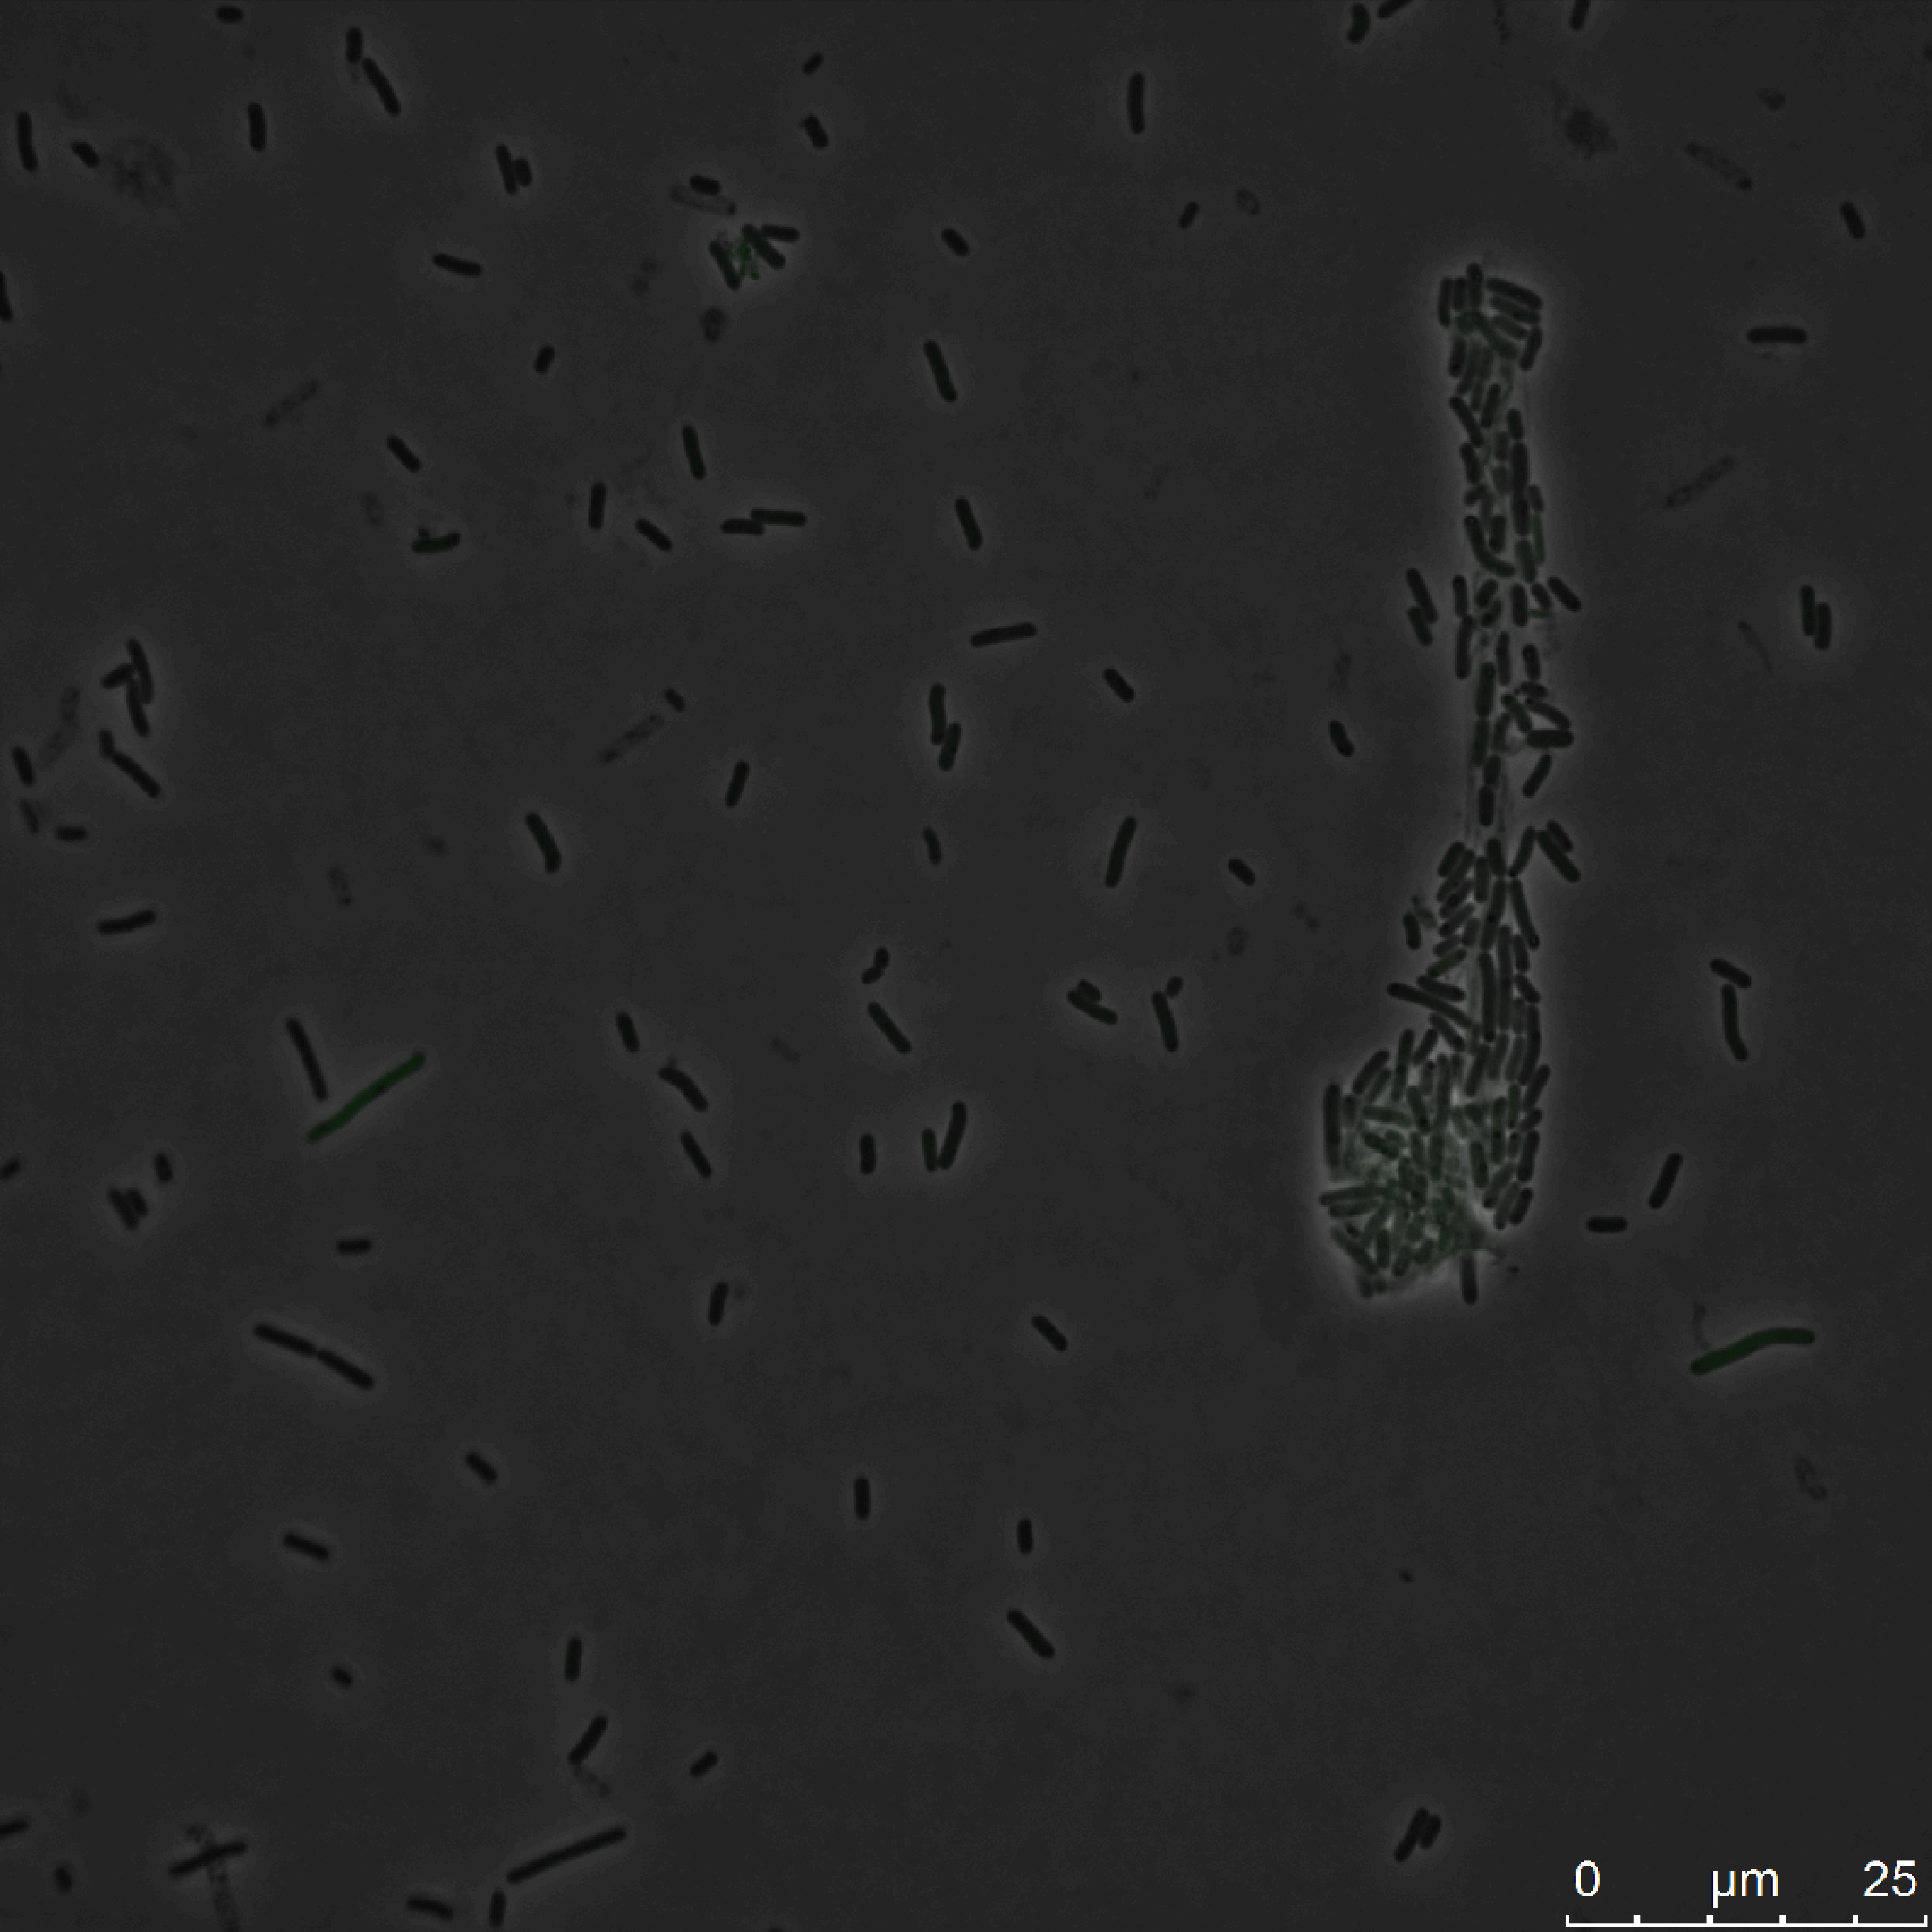
\includegraphics{TT01U1_24HR_2_LOWGREEN.pdf} &%
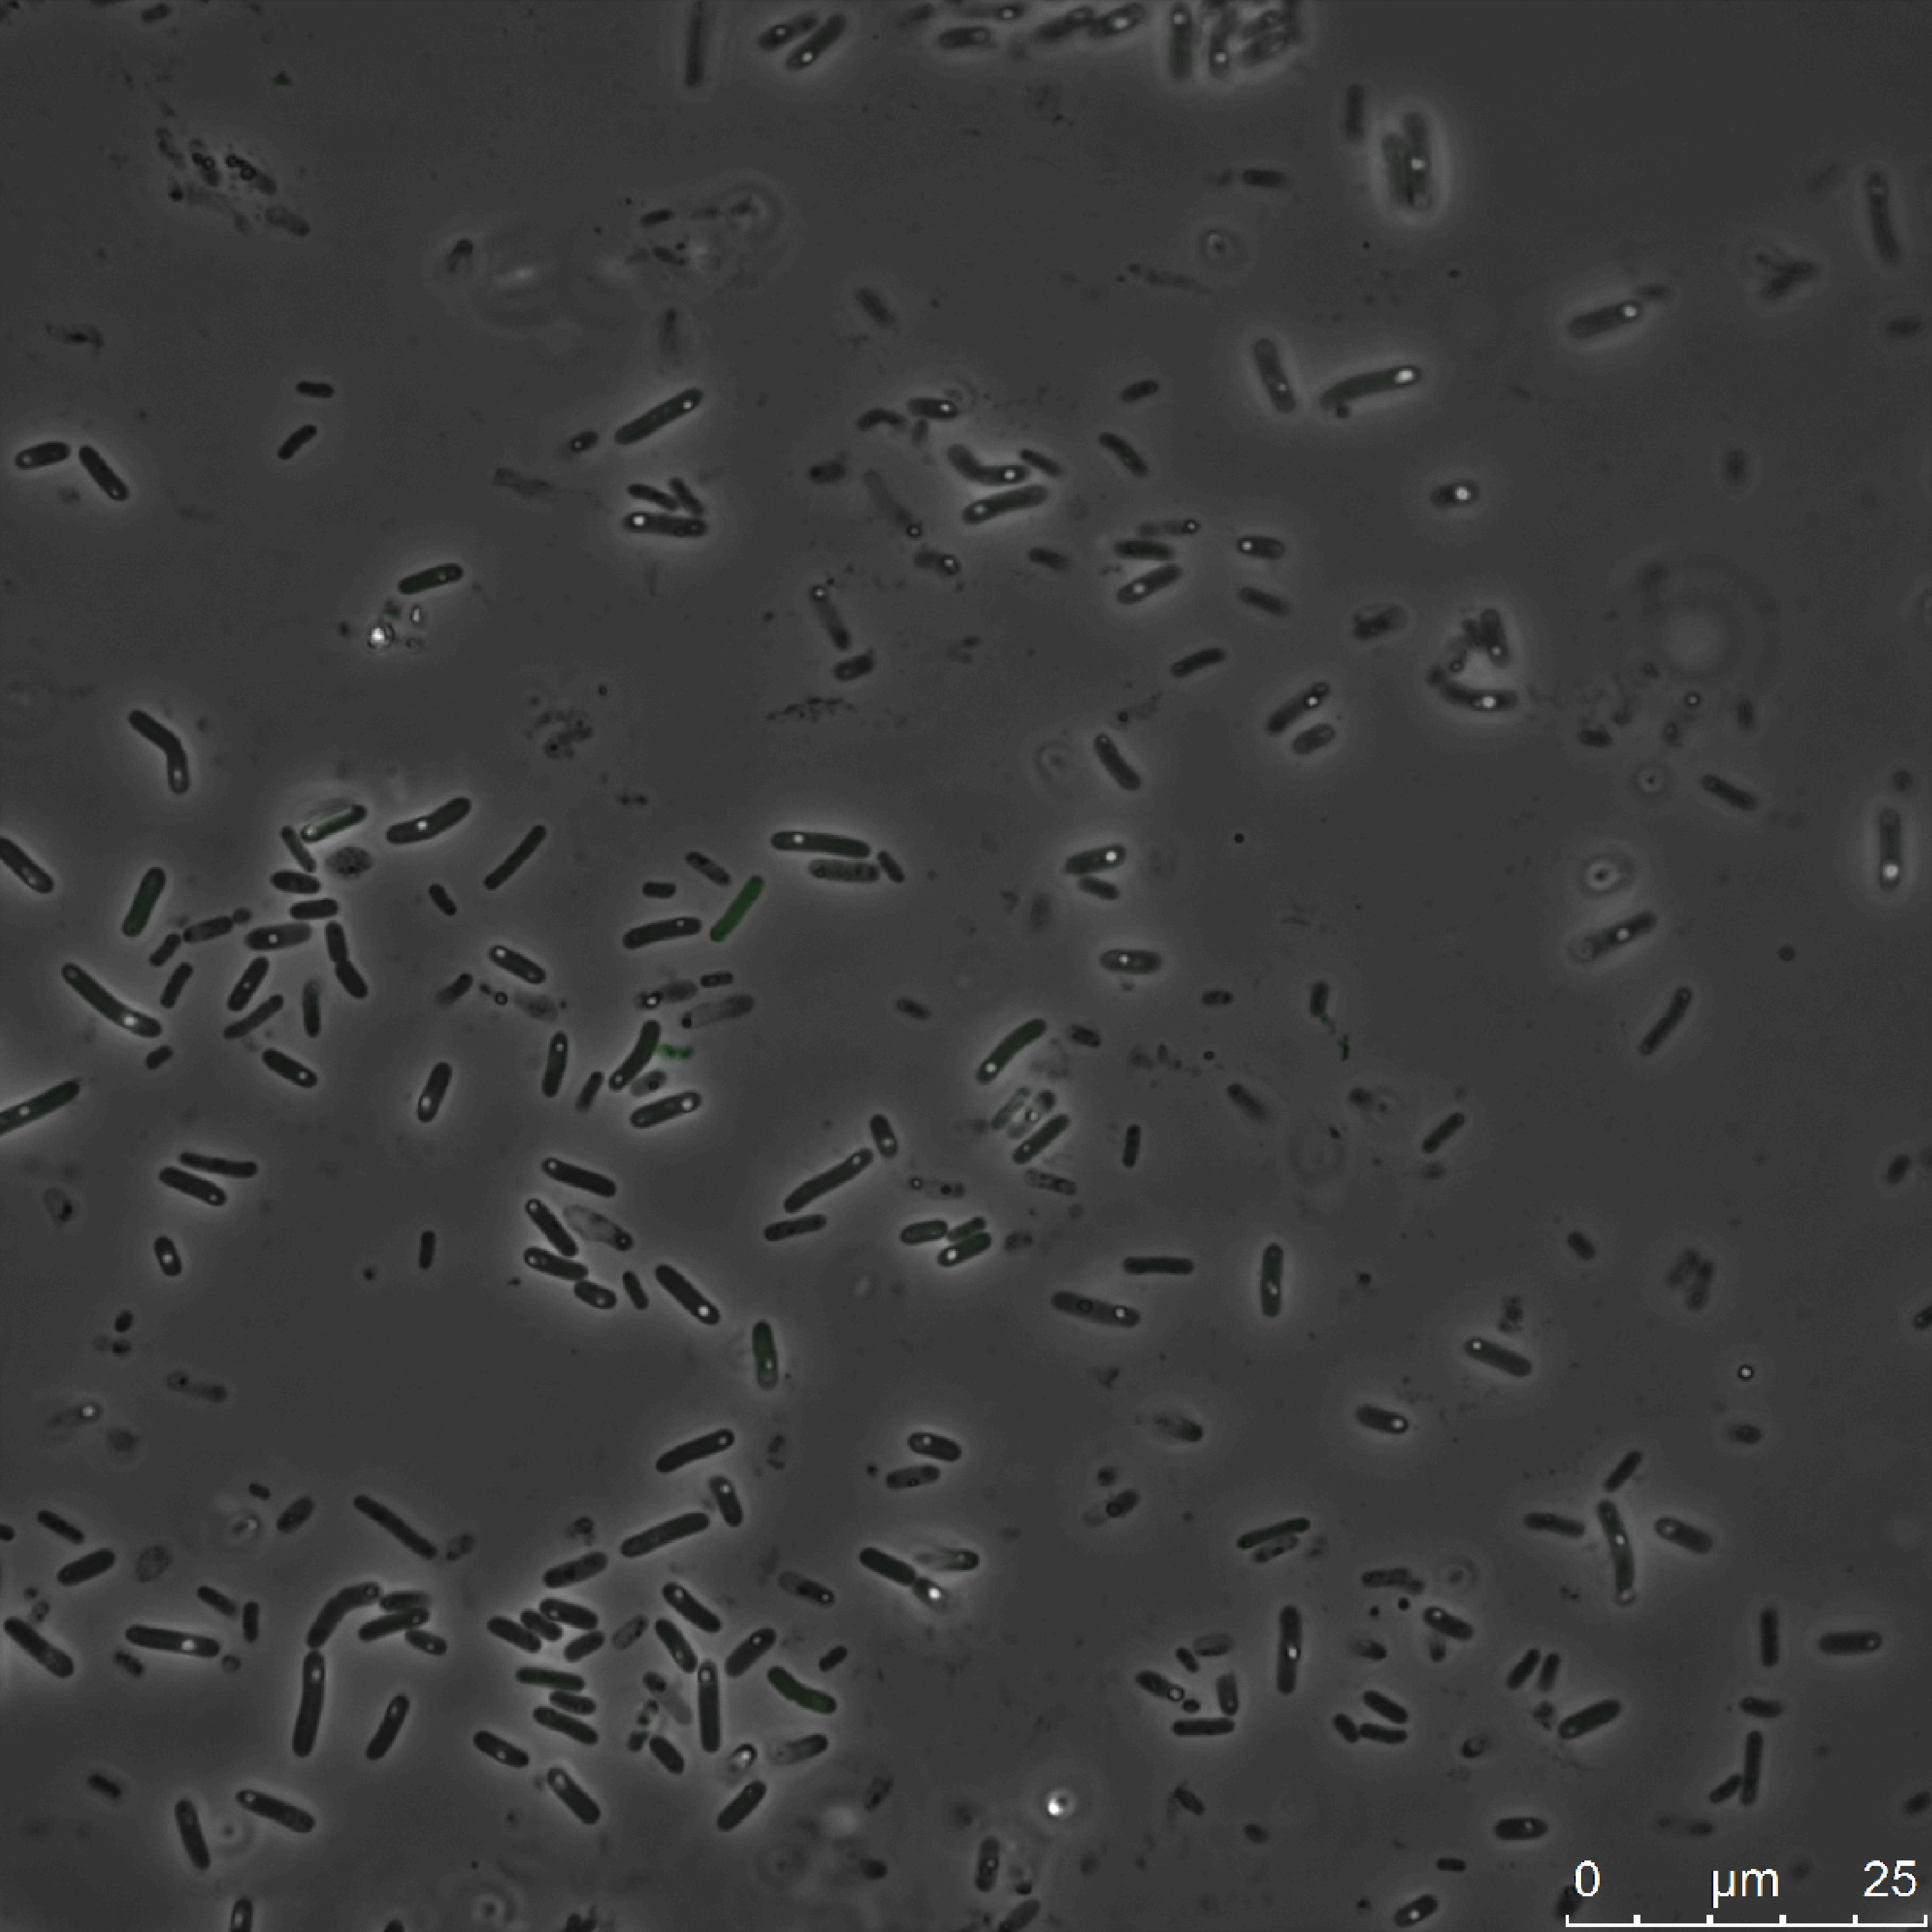
\includegraphics{TT01U1_72HR_2_LOWGREEN.pdf} \\[-0.5ex]

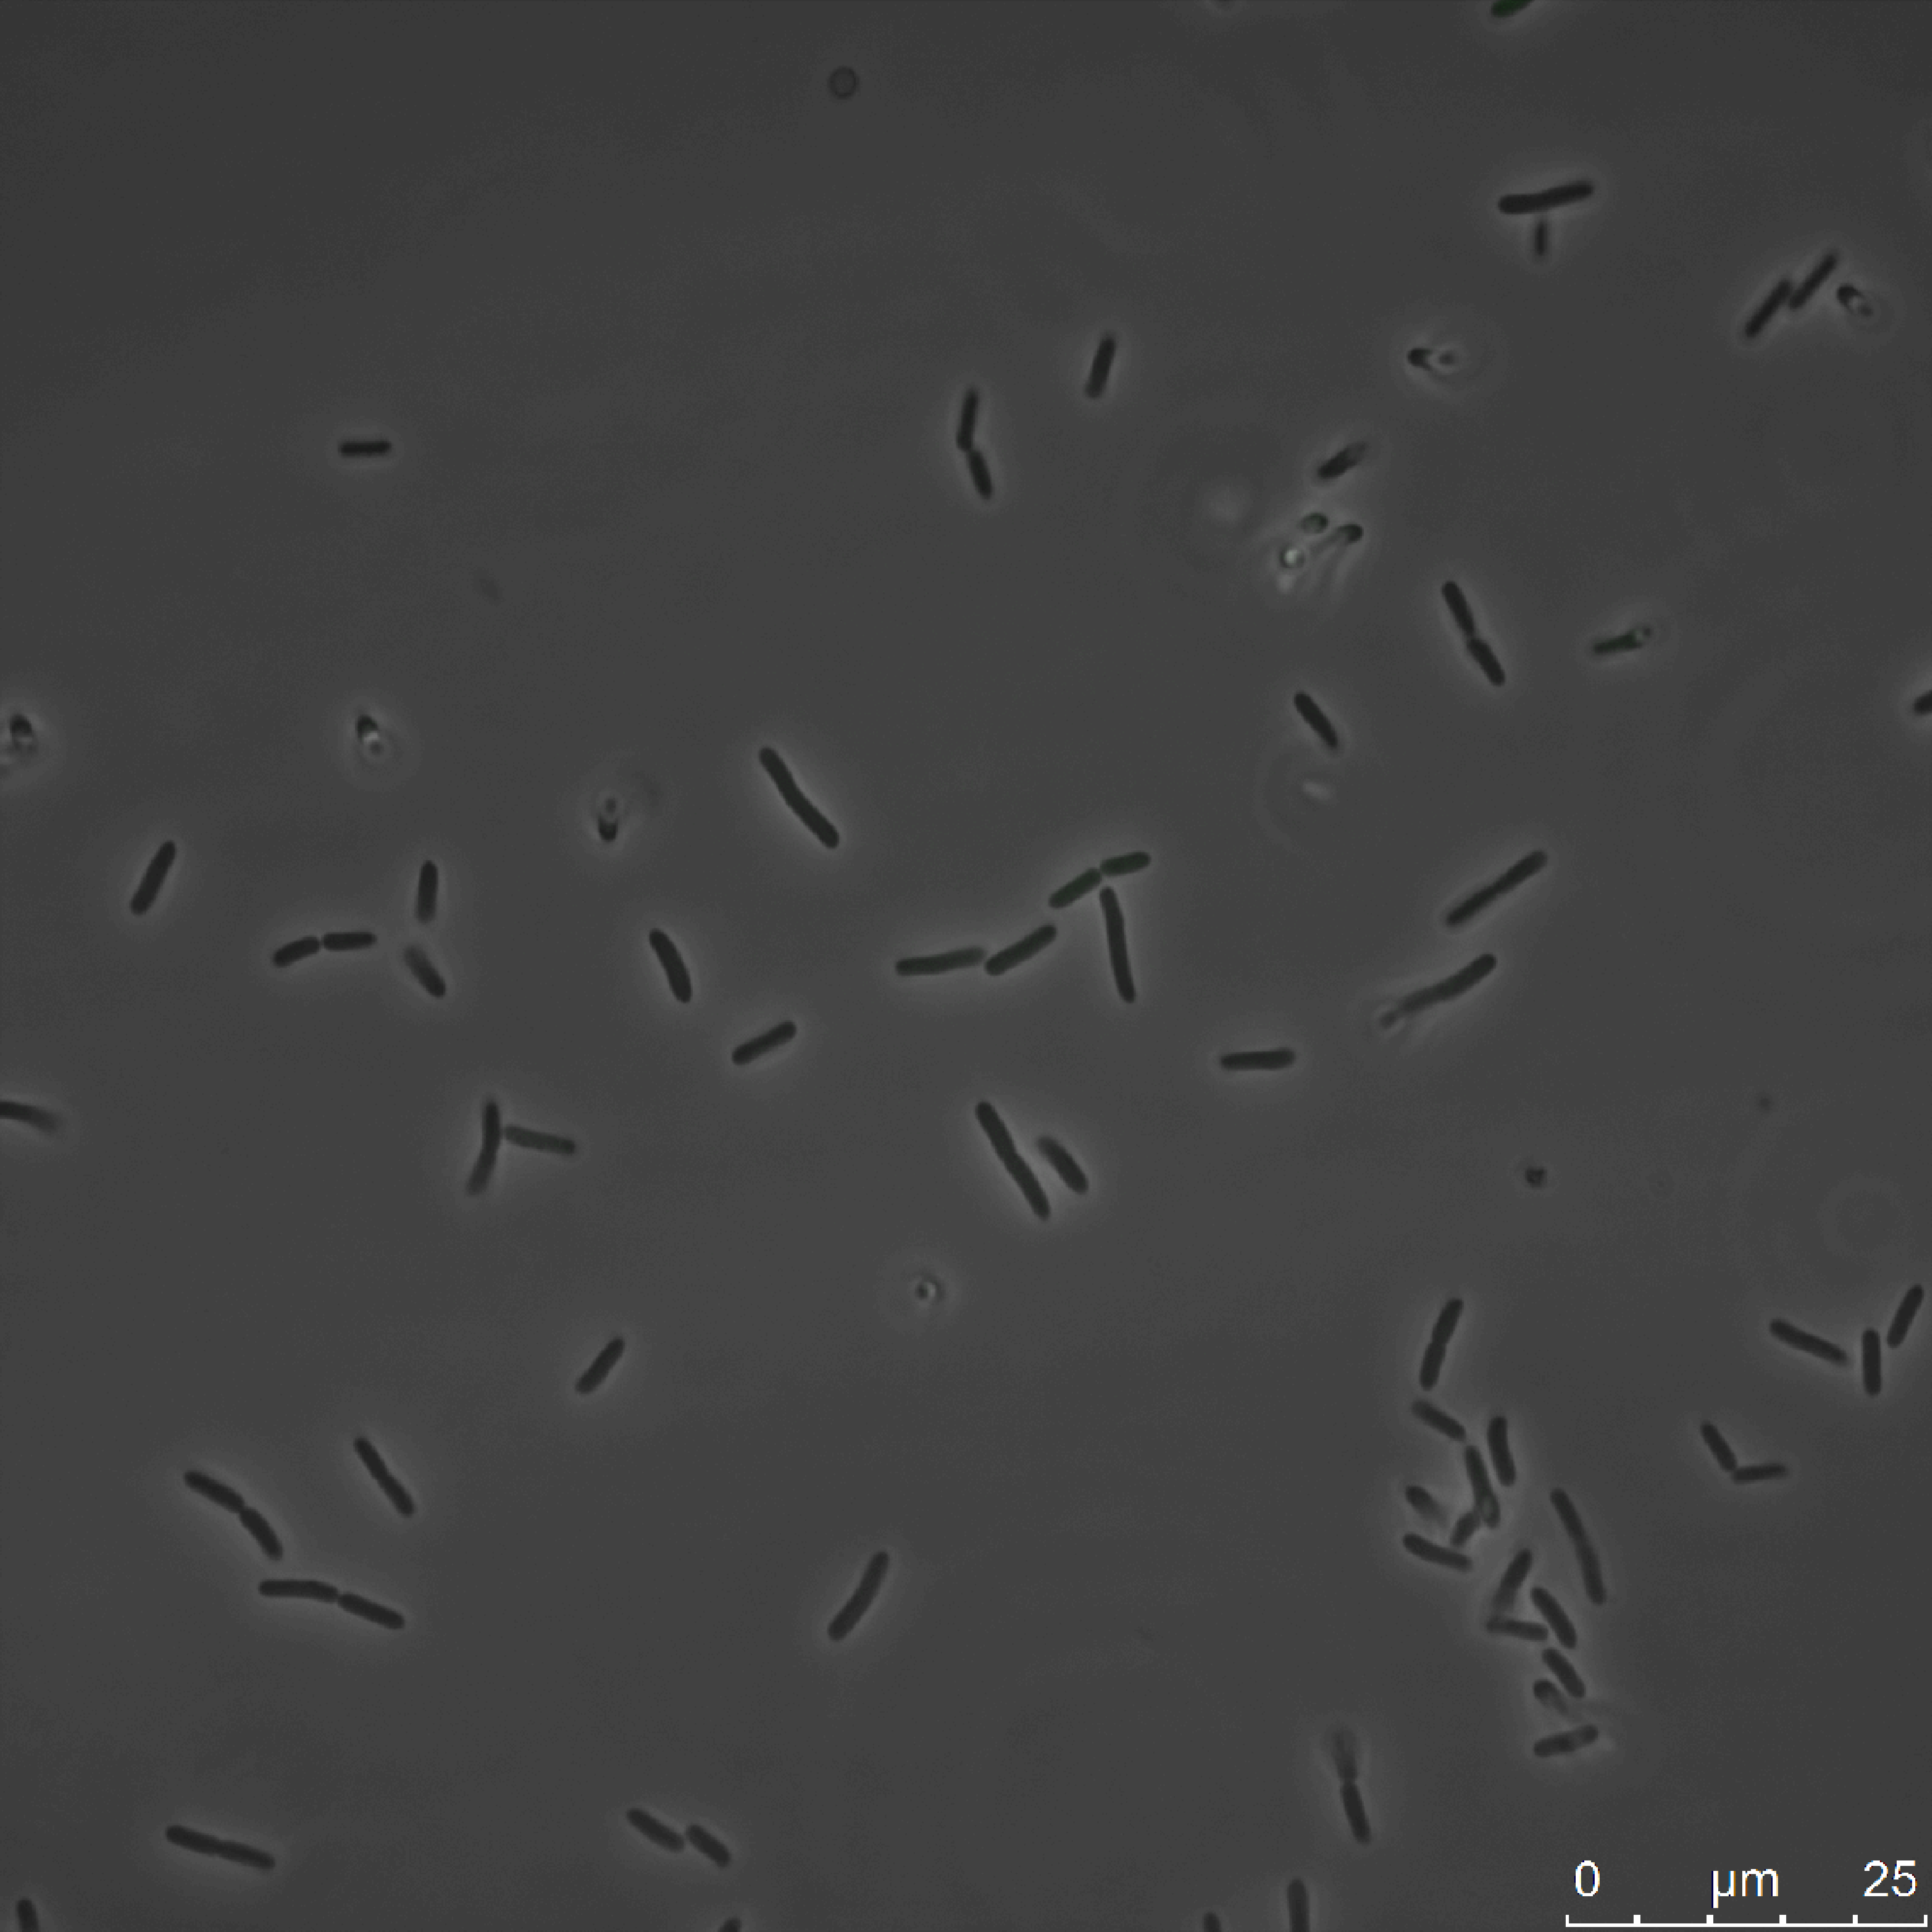
\includegraphics{TT01U1_3_NOGREEN.pdf} &%
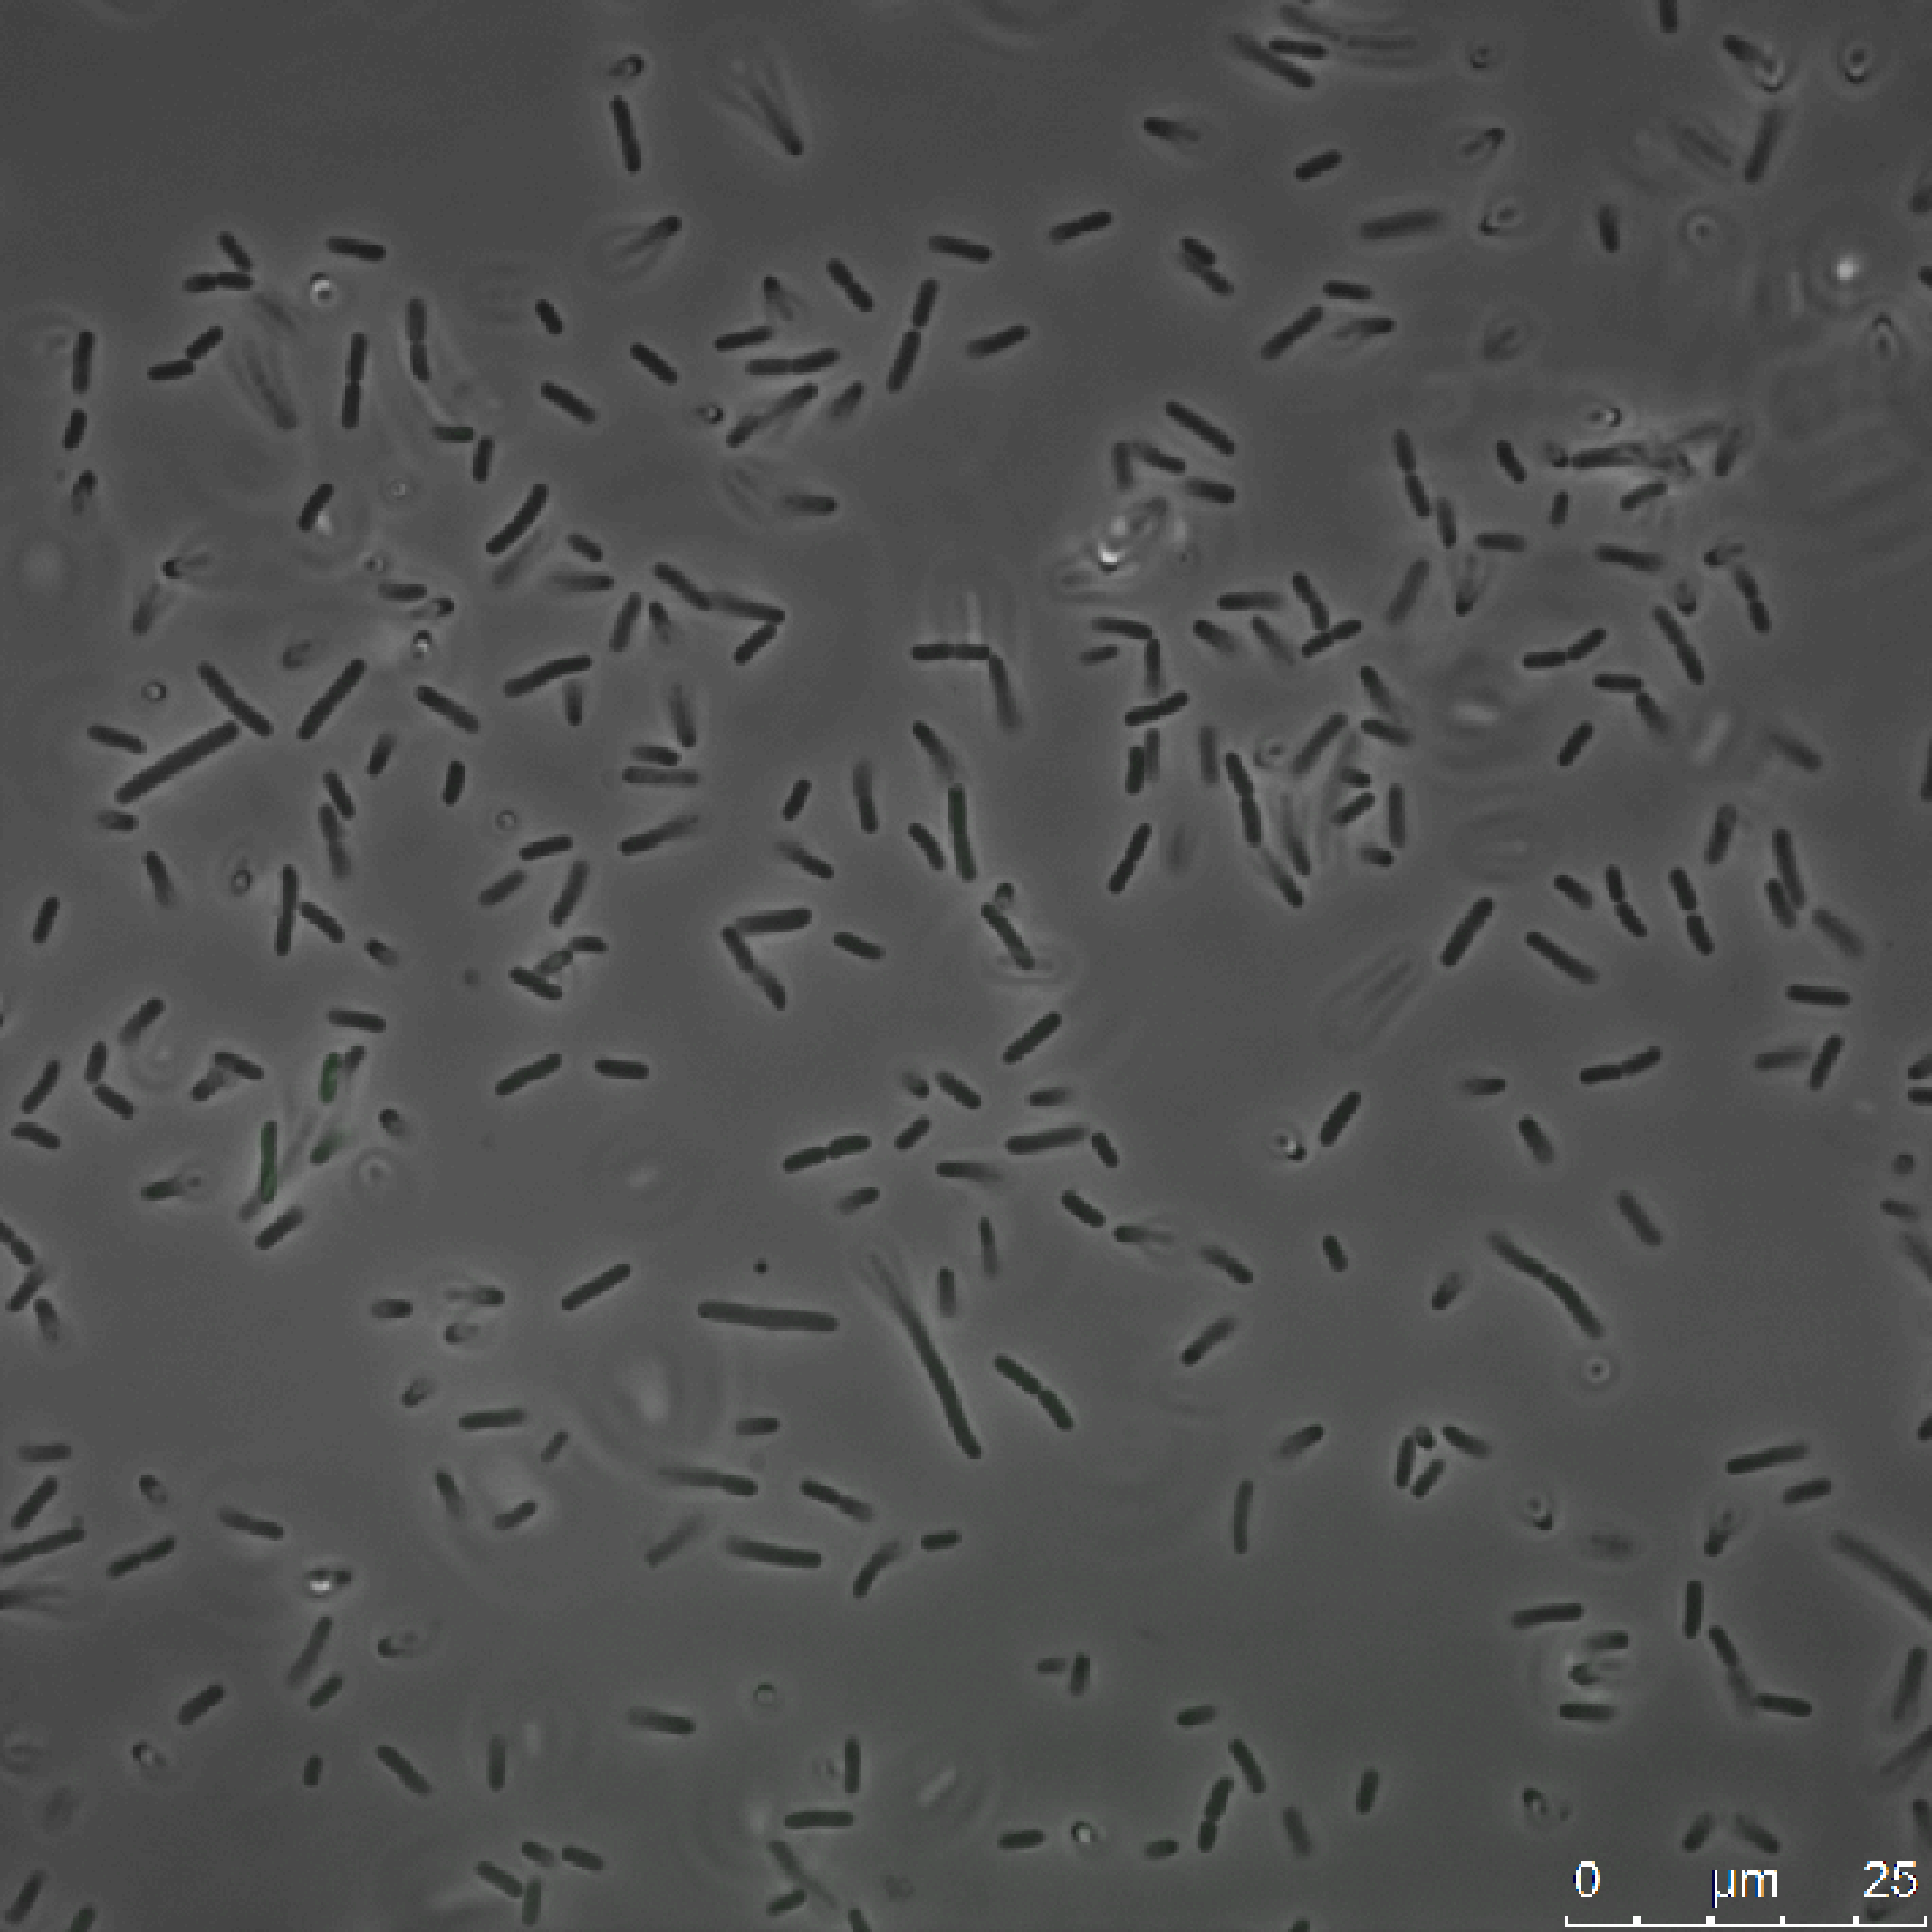
\includegraphics{TT01U1_5HR_3_LOWGREEN.pdf} &%
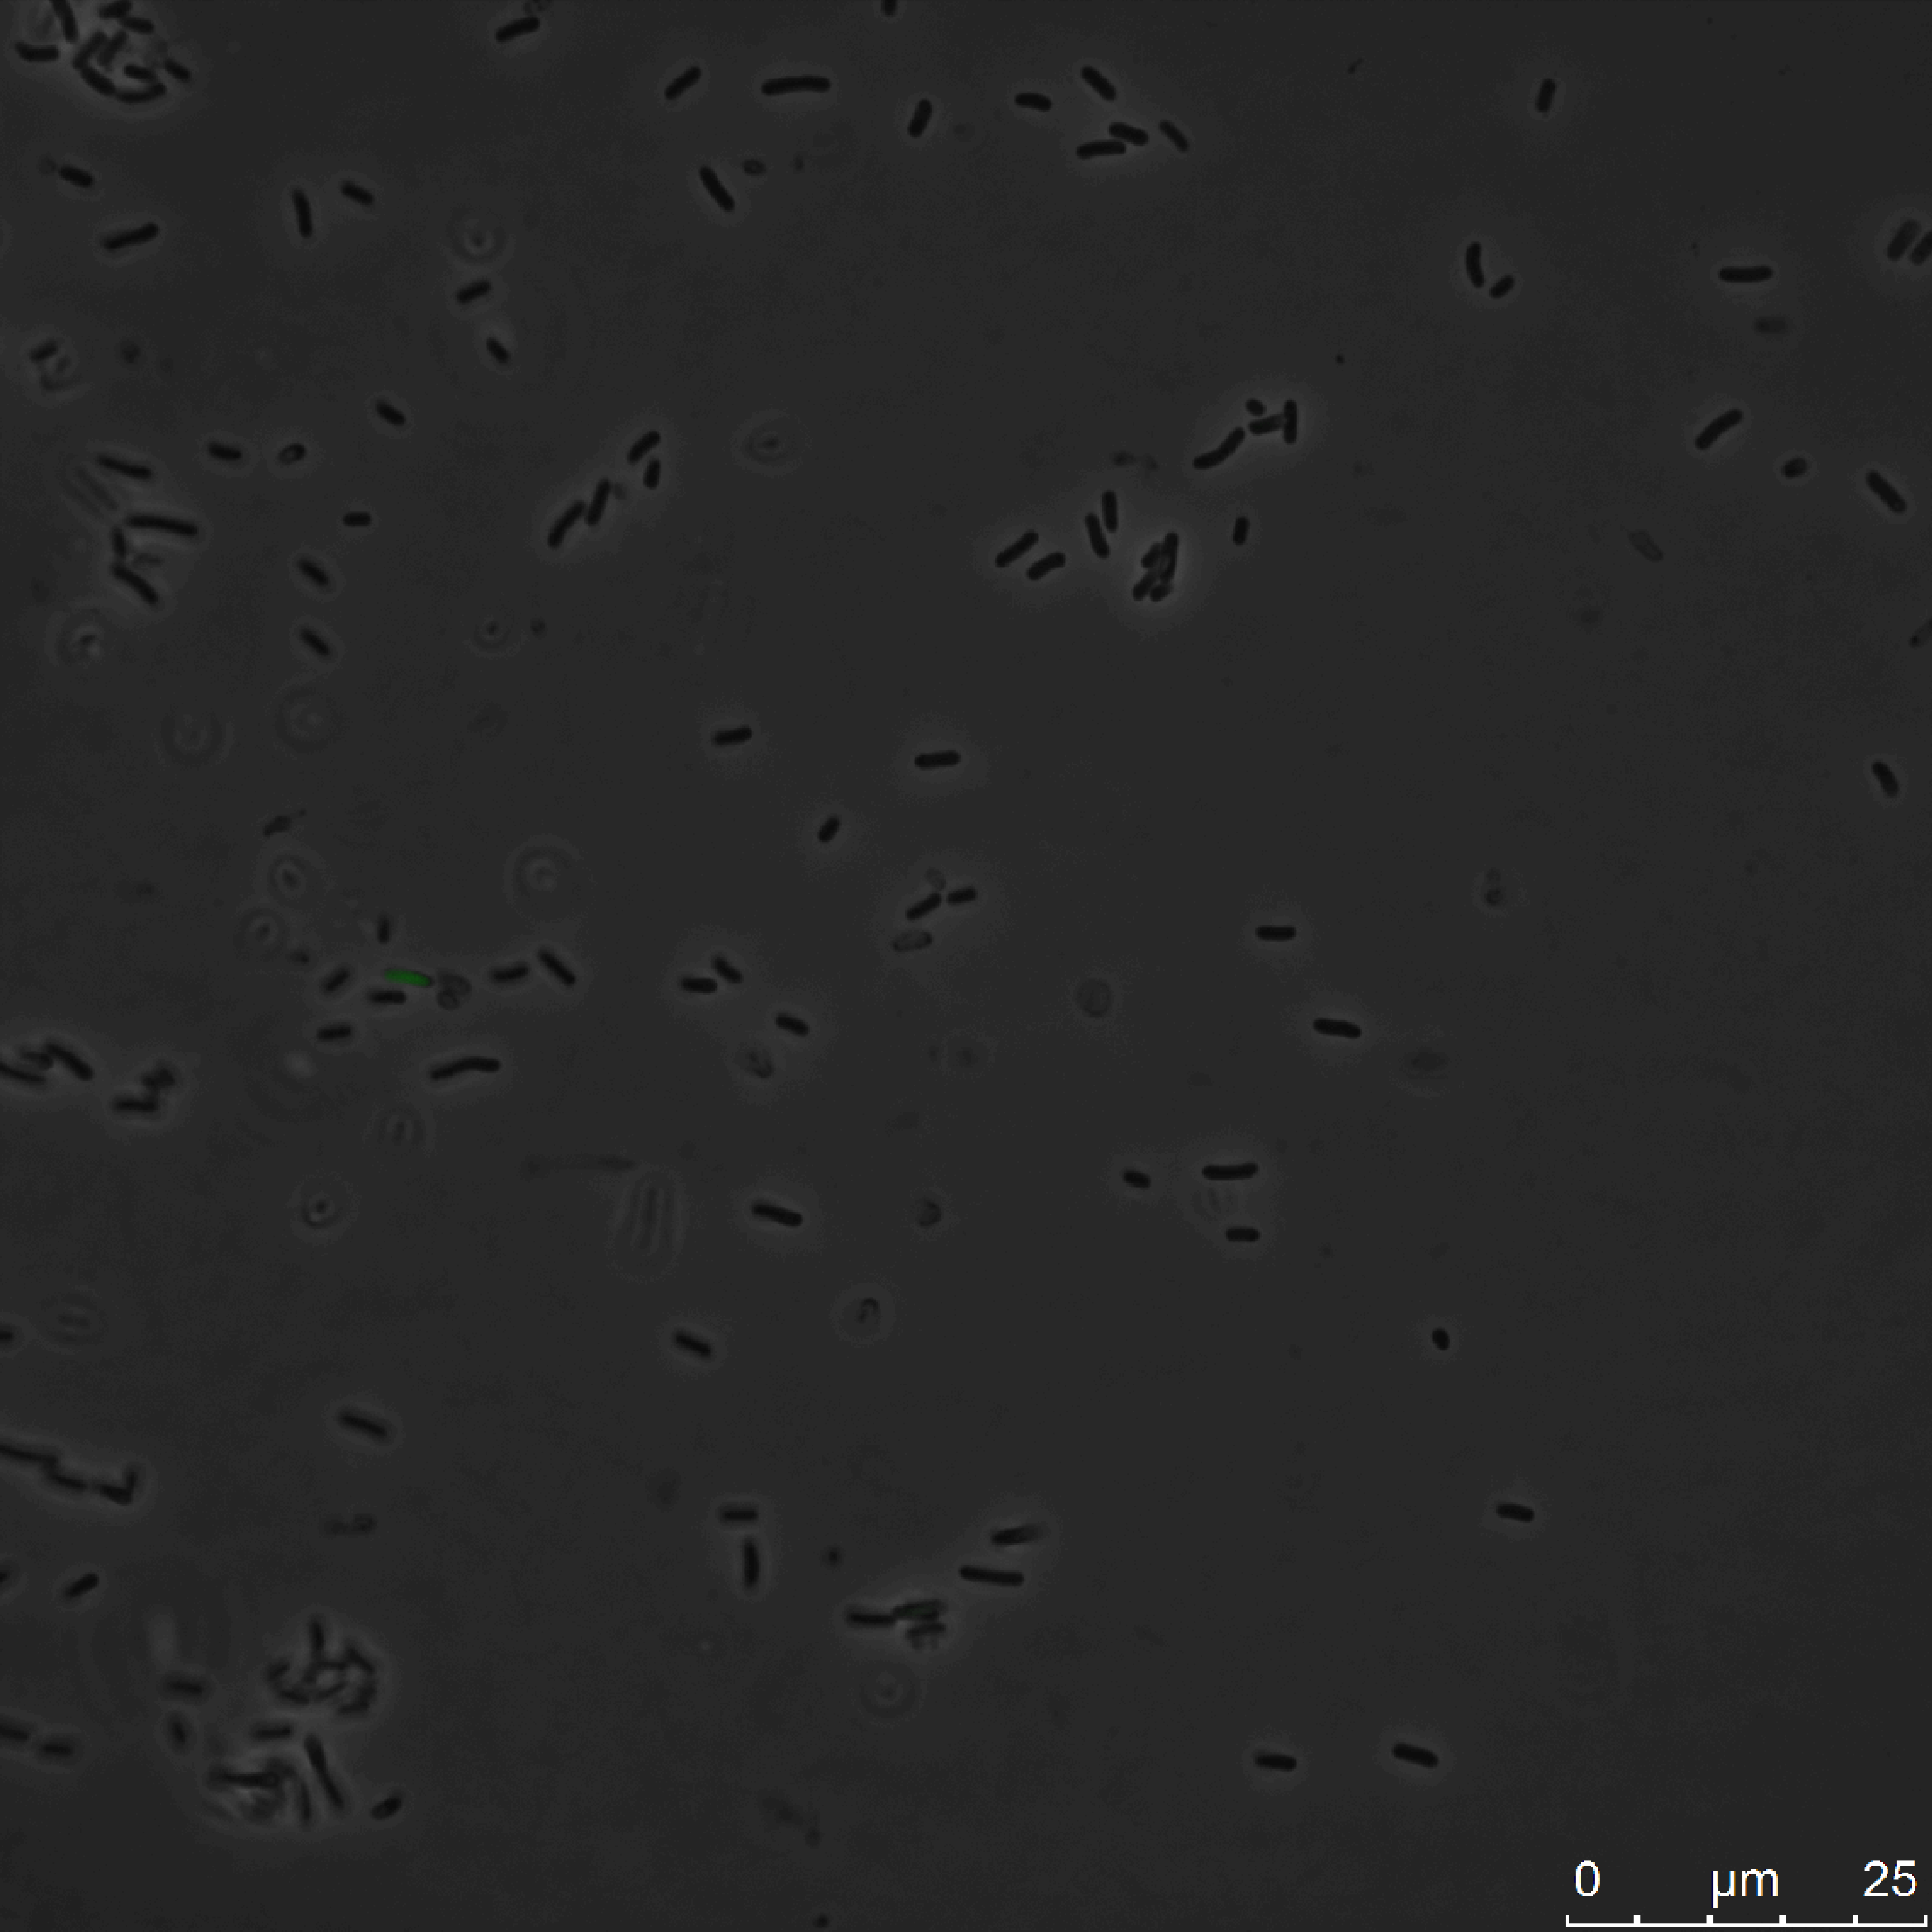
\includegraphics{TT01U1_24HR_3_GREEN.pdf} &%
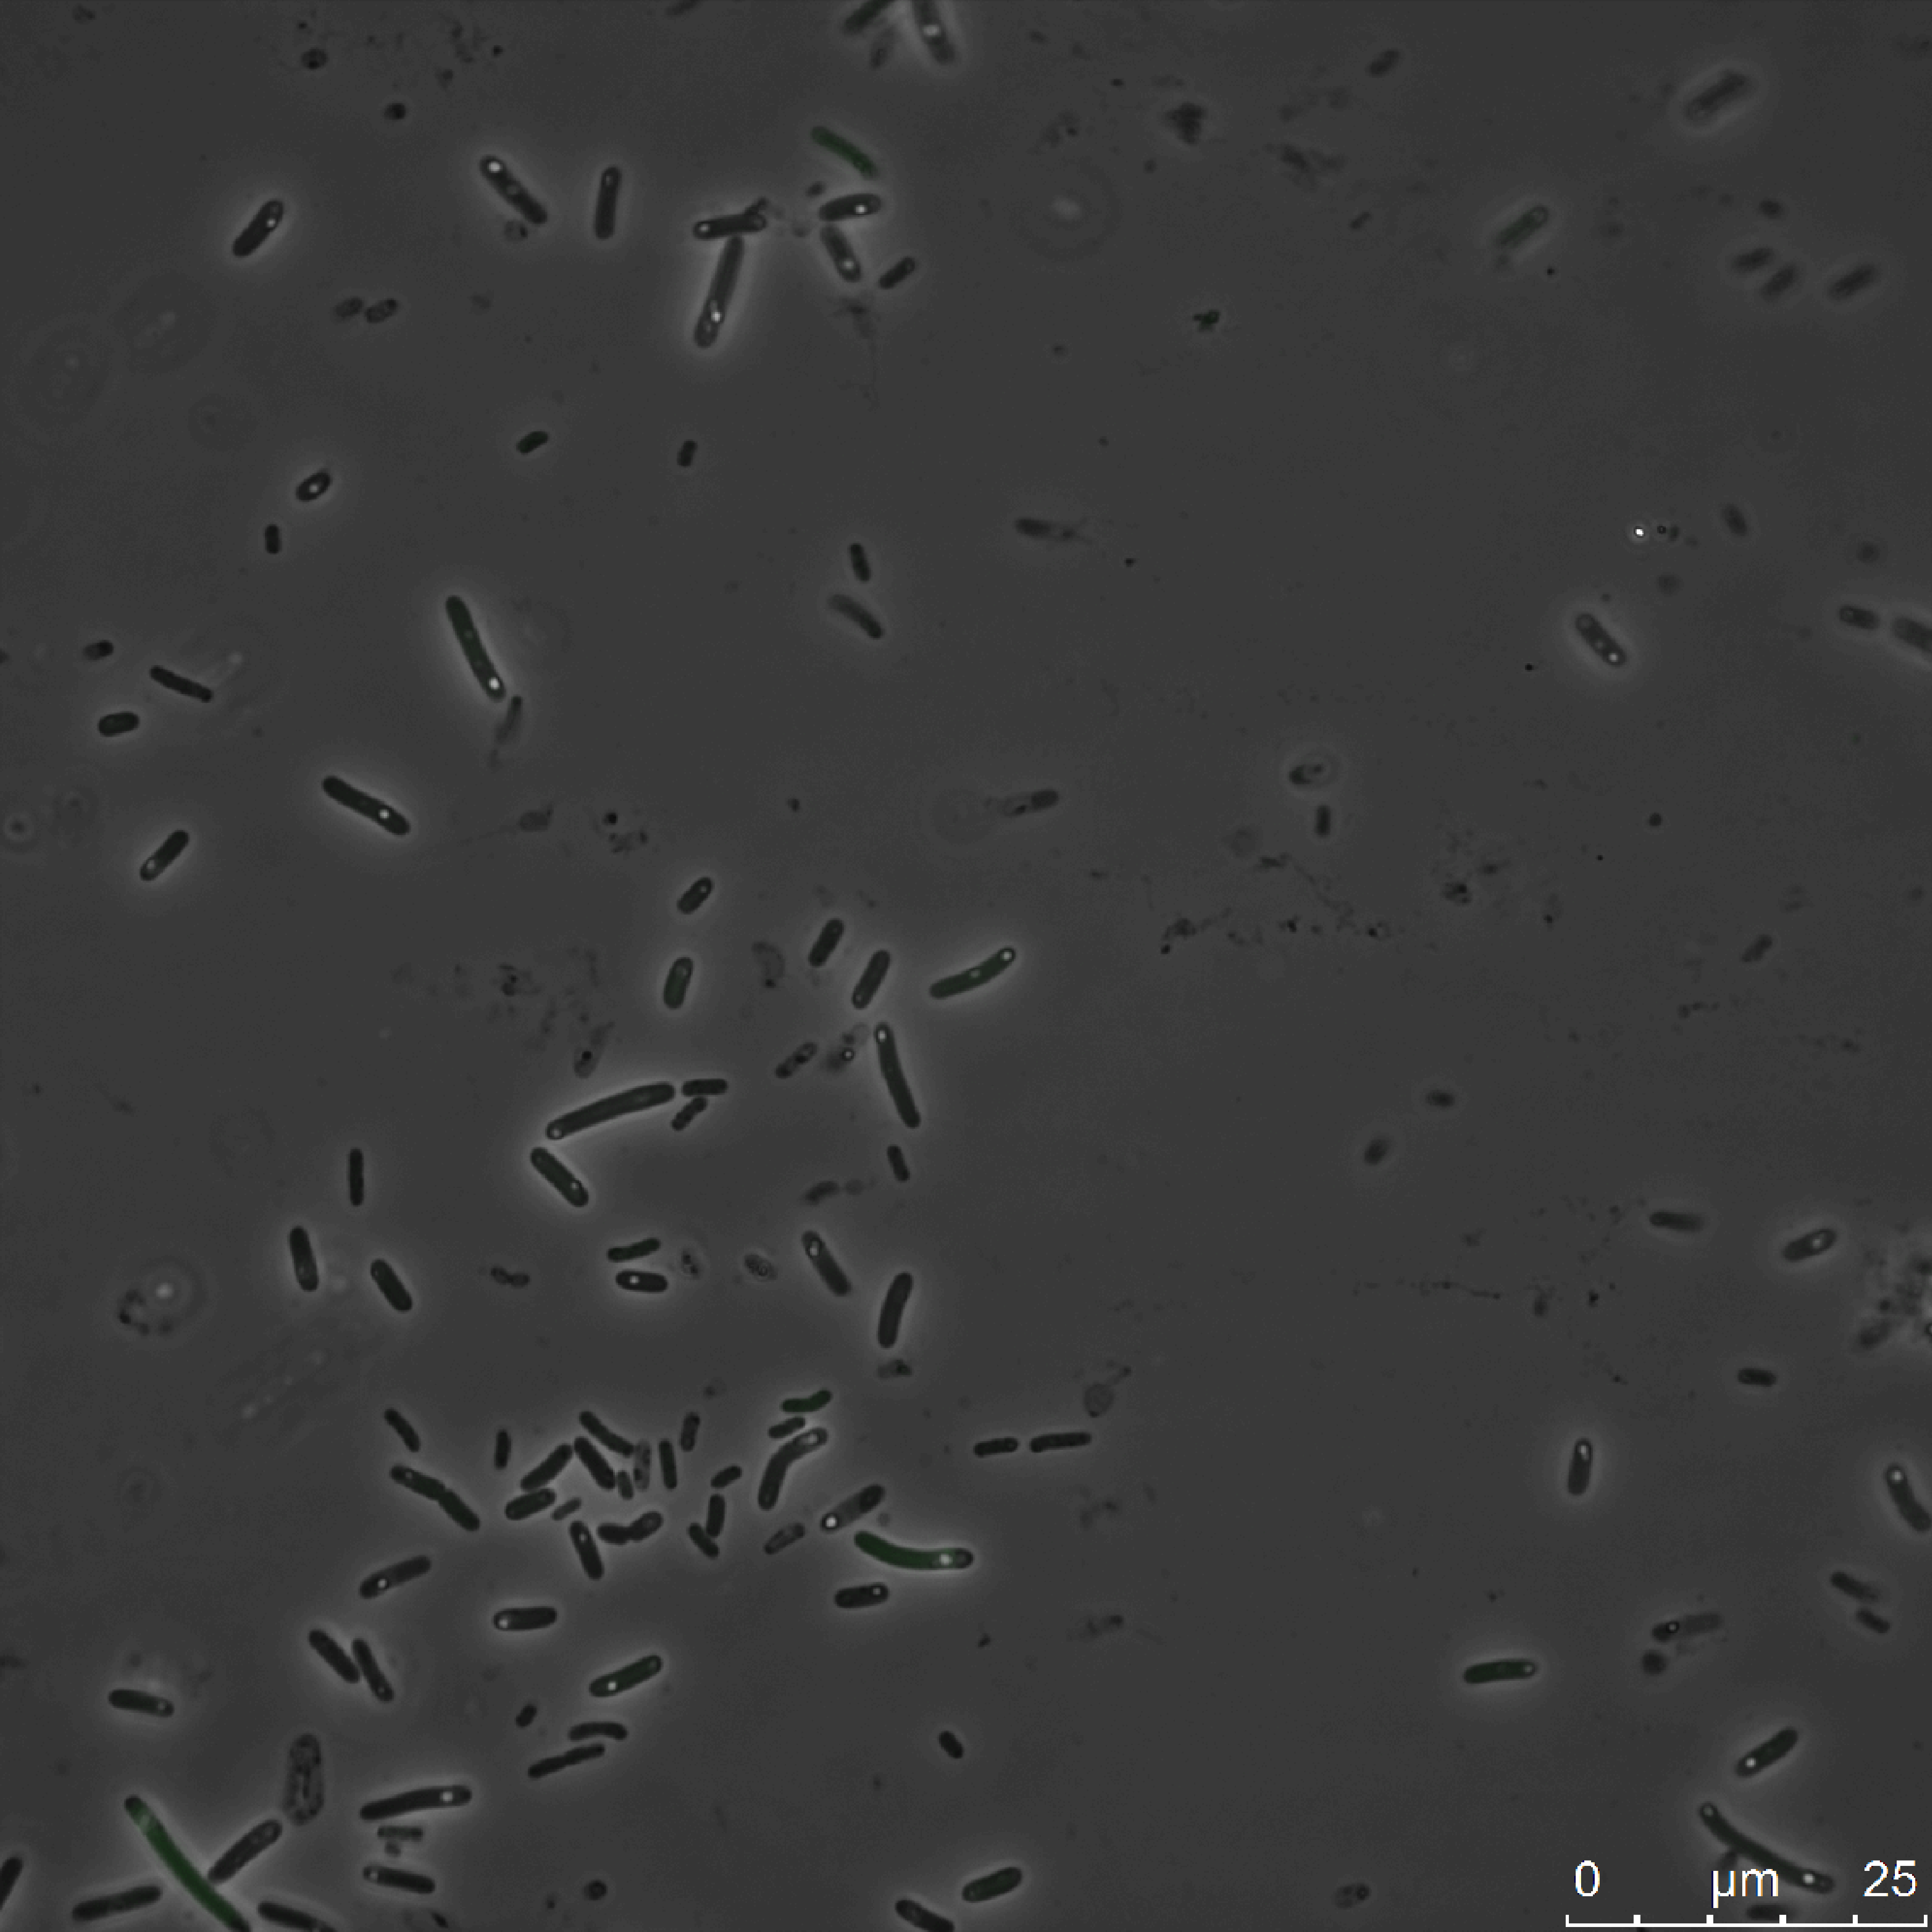
\includegraphics{TT01U1_72HR_3_LOWGREEN.pdf} \\[-0.5ex]

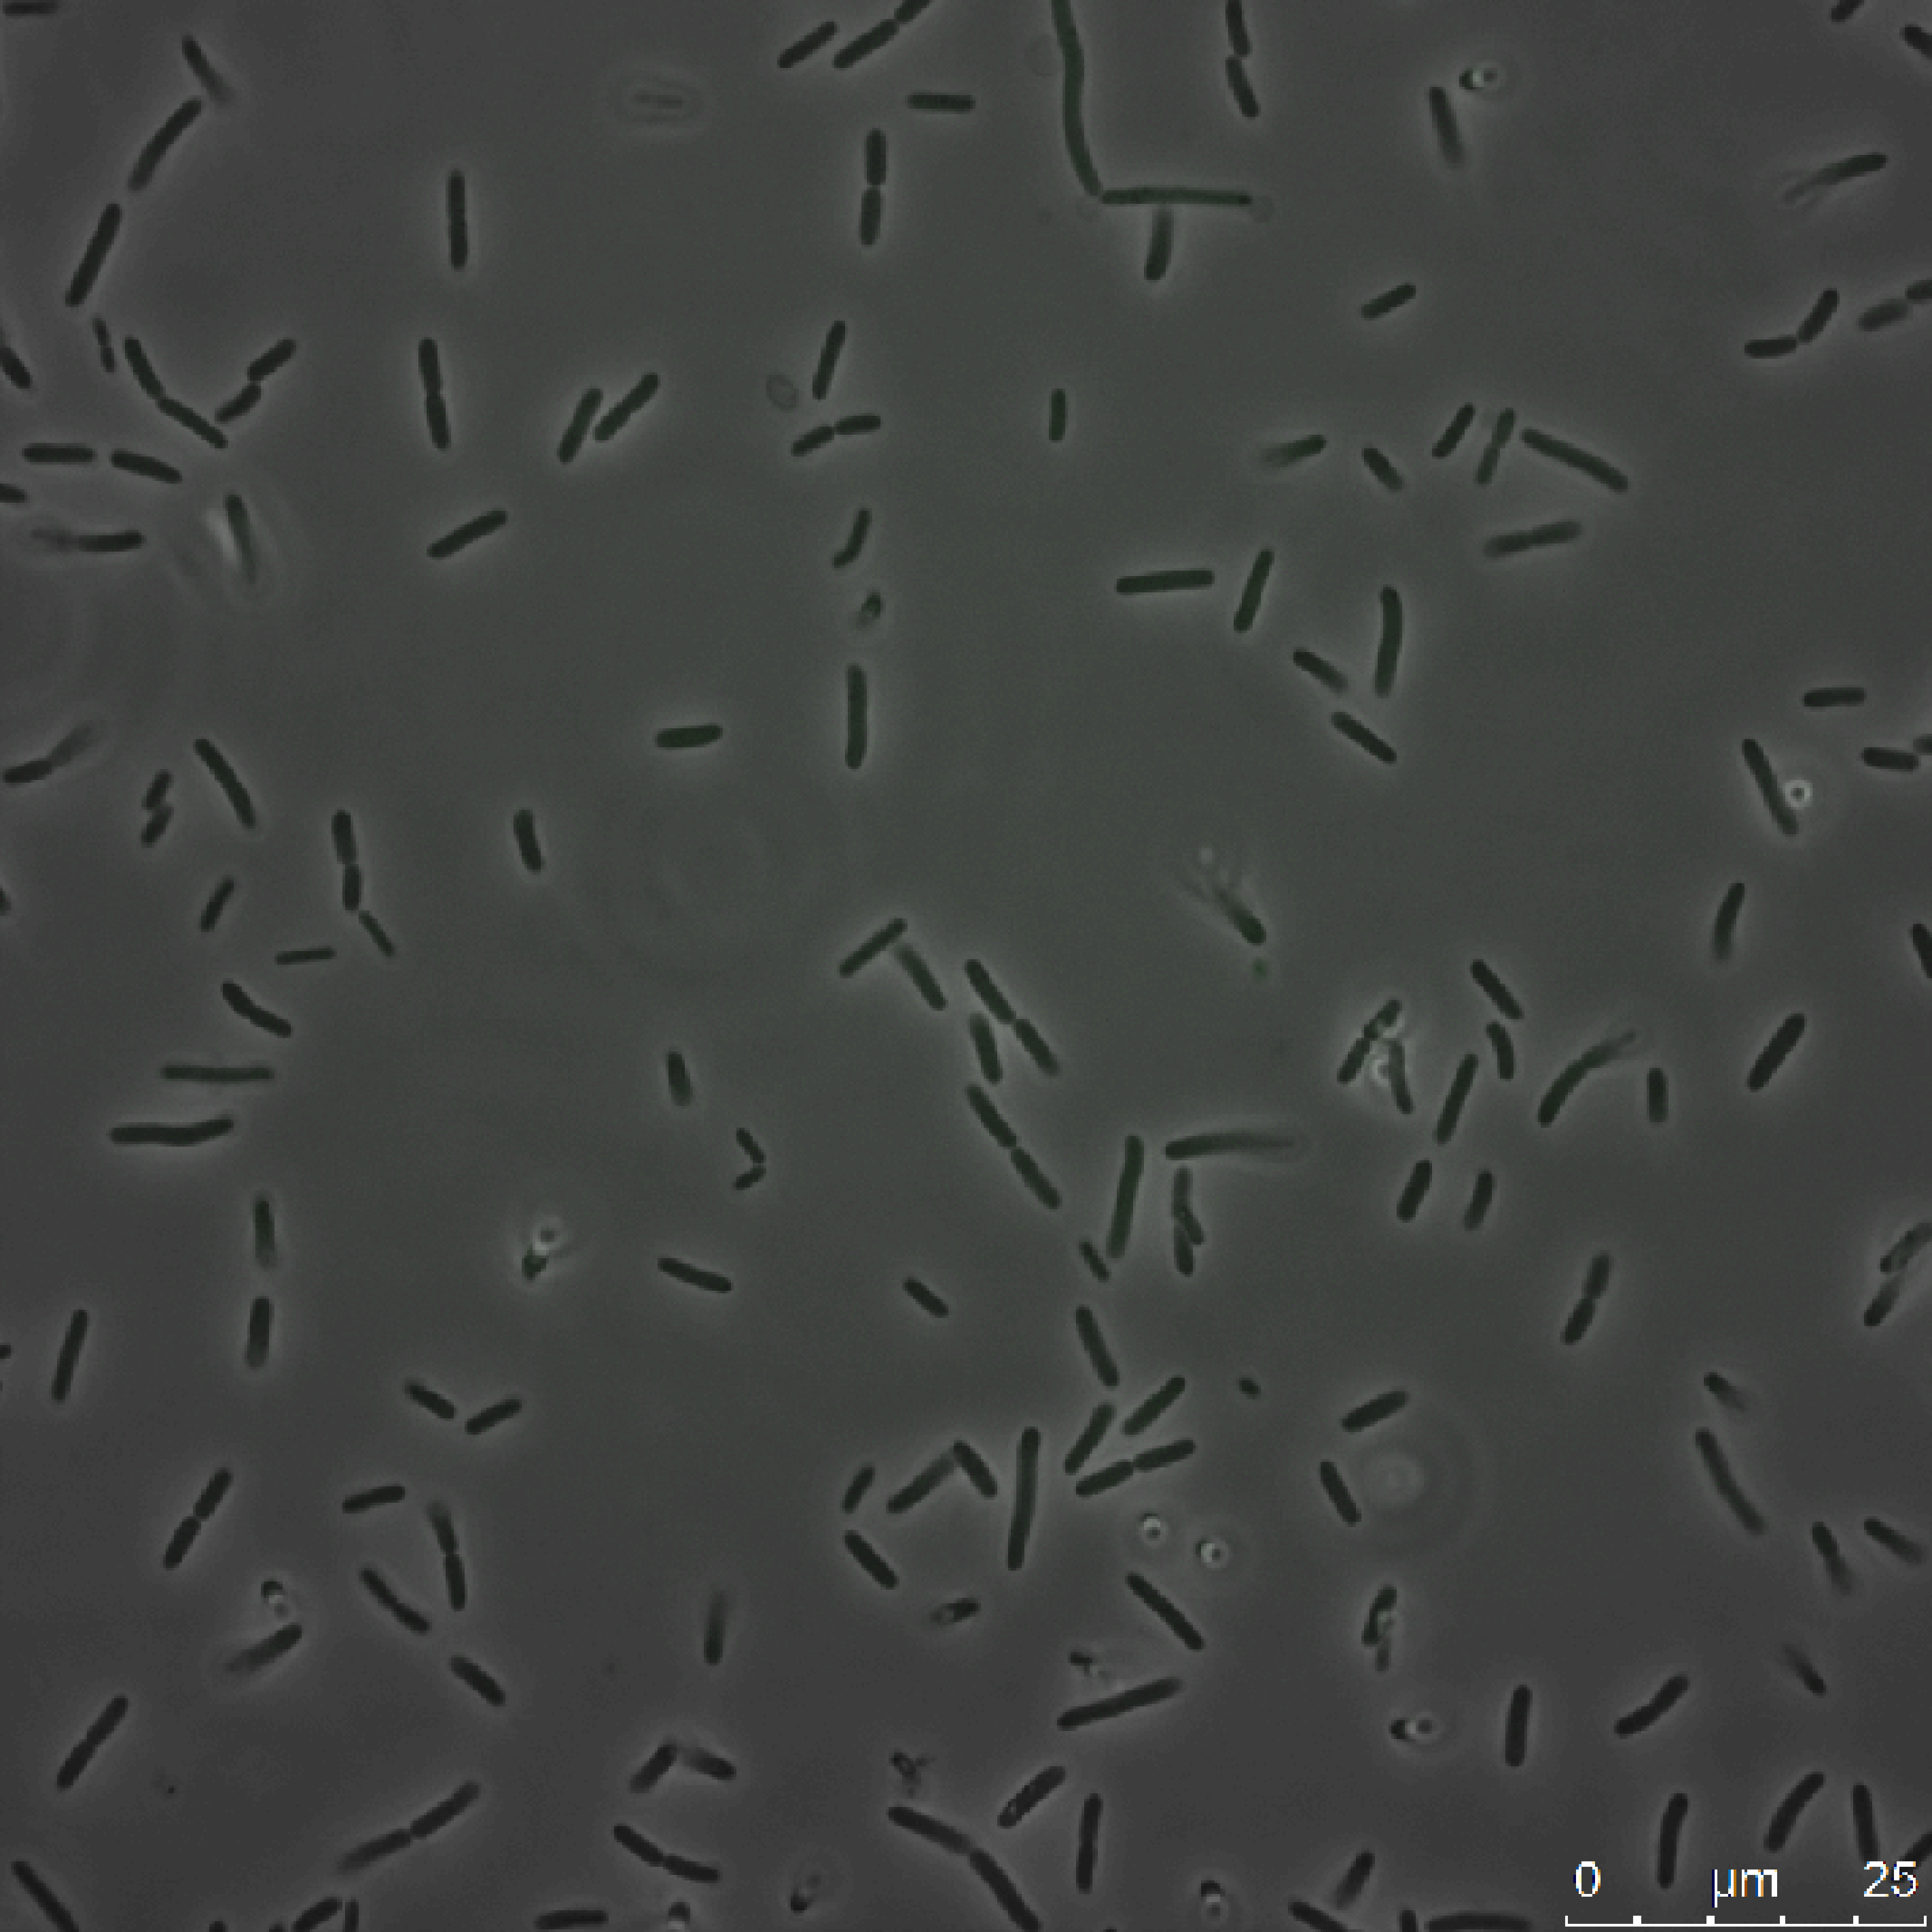
\includegraphics{TT01U1_4_NOGREEN.pdf} &%
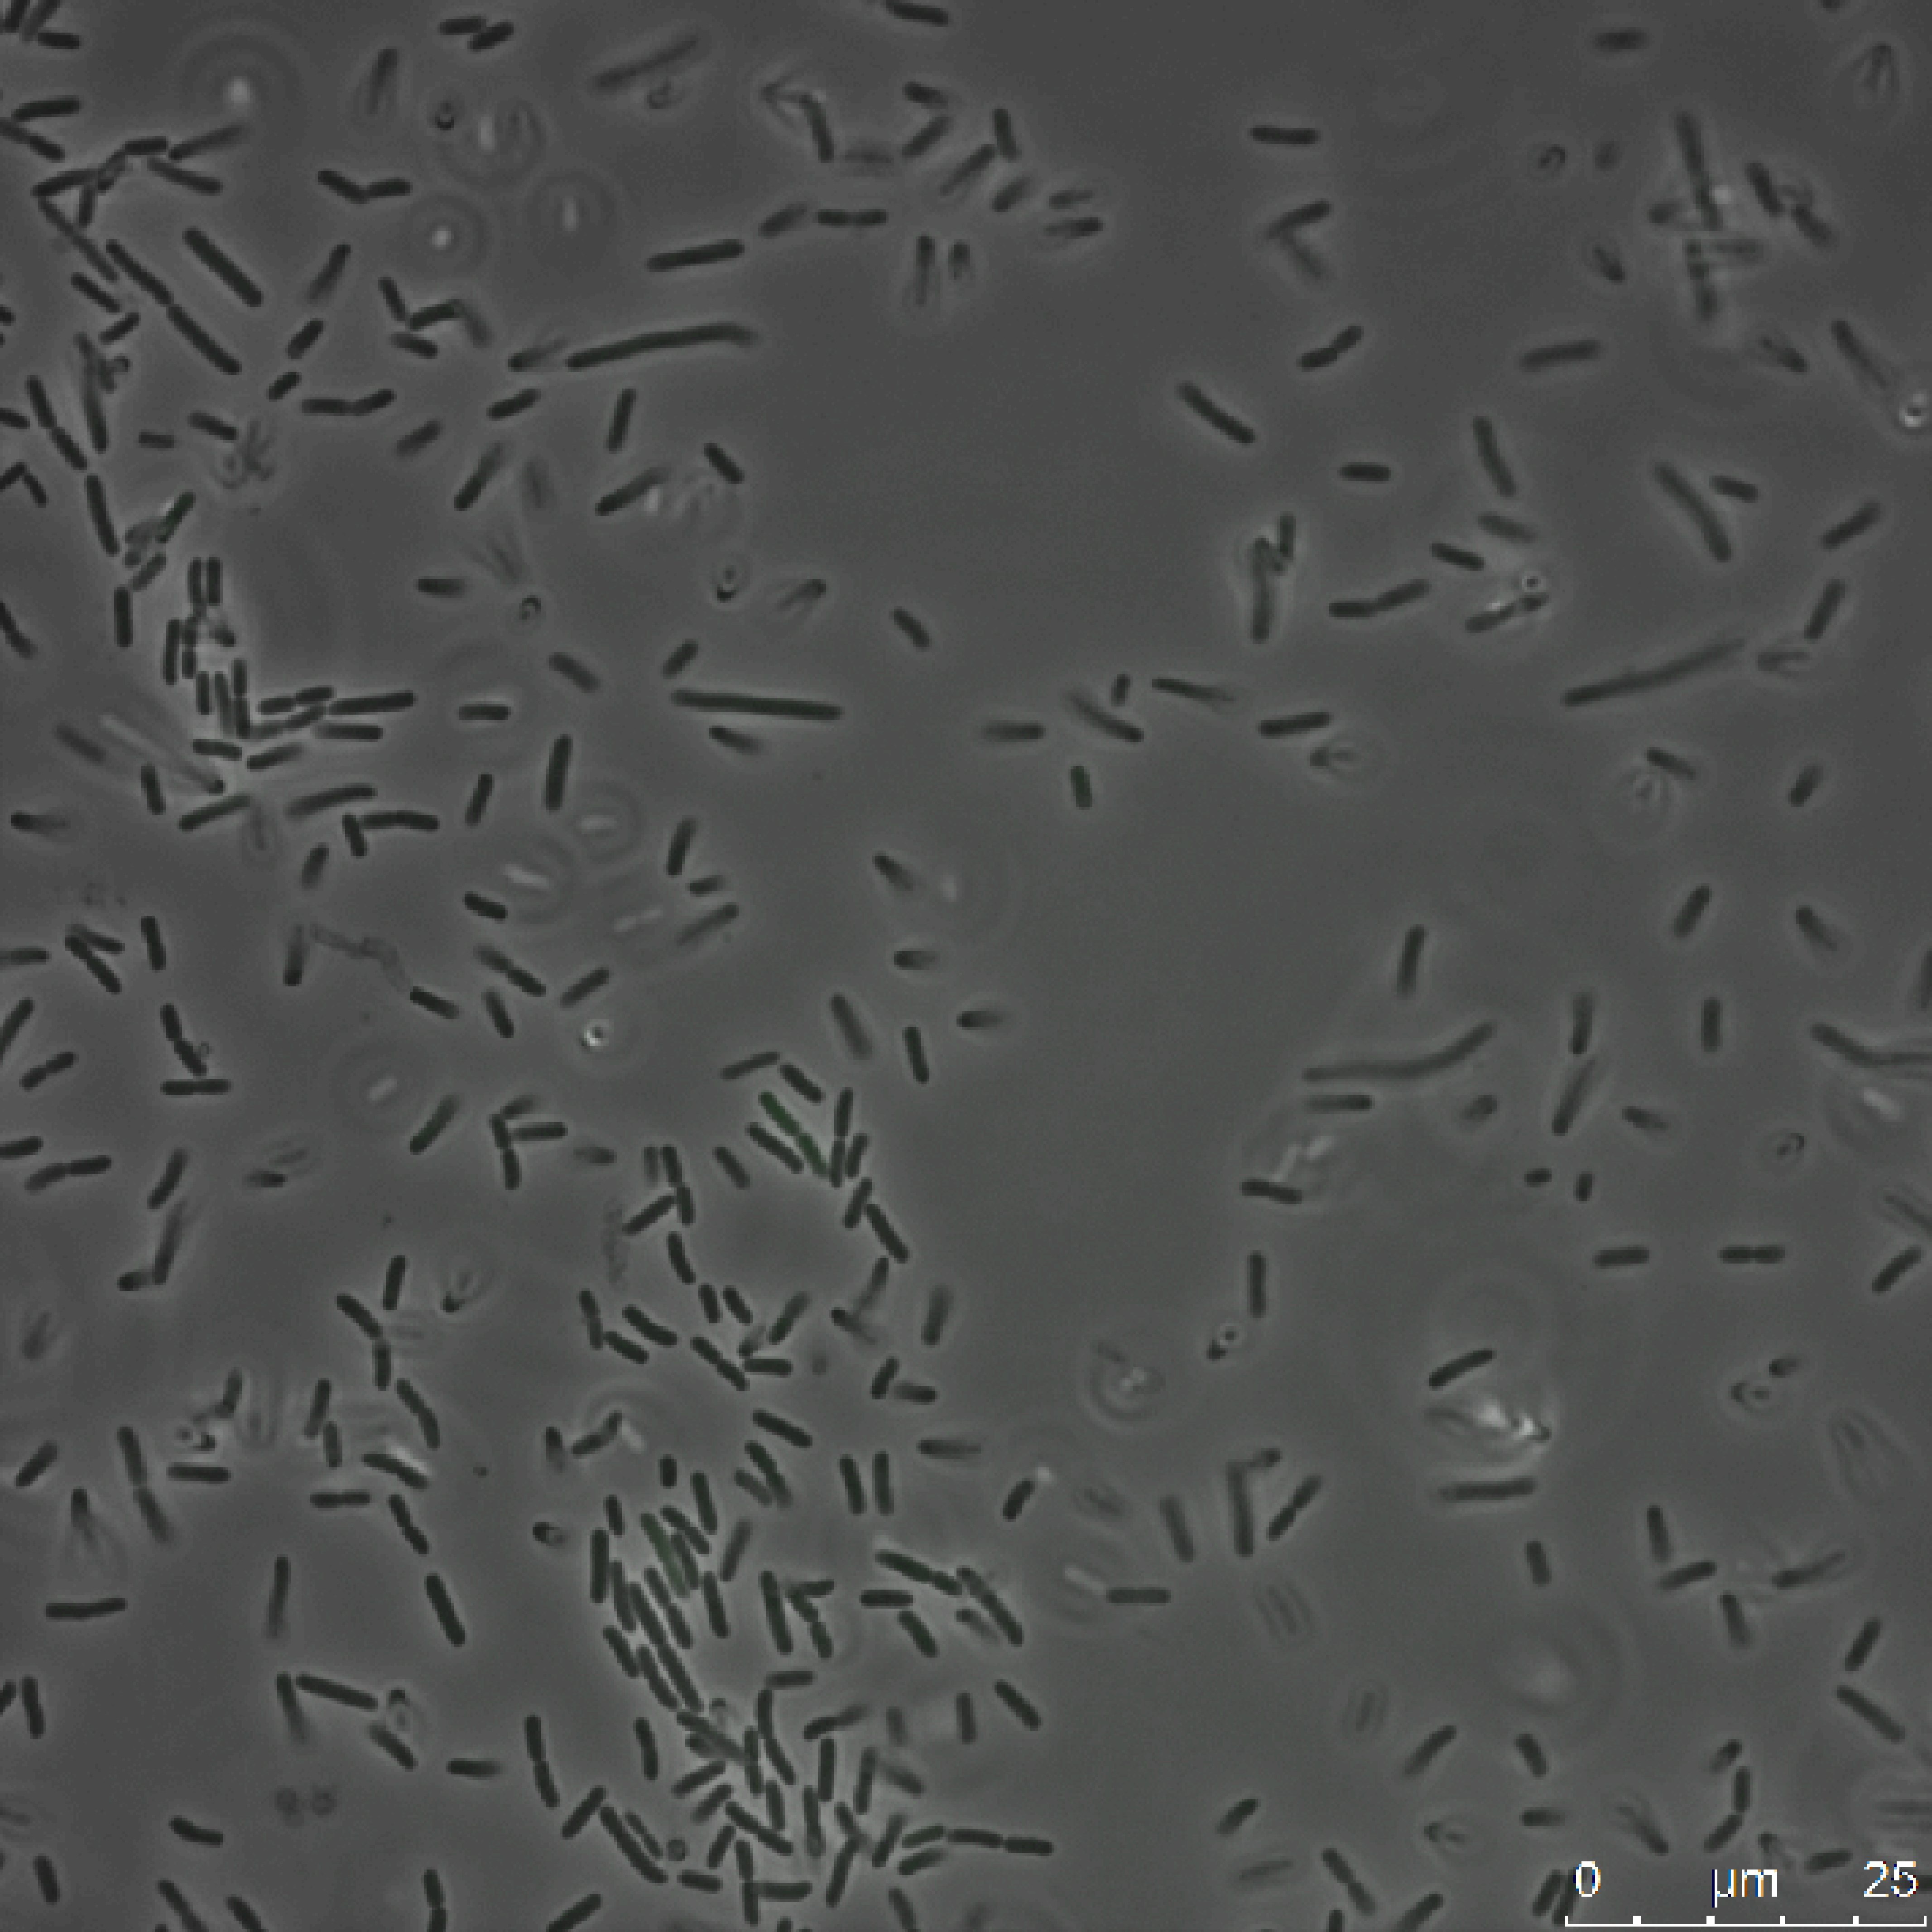
\includegraphics{TT01U1_5HR_4_LOWGREEN.pdf} &%
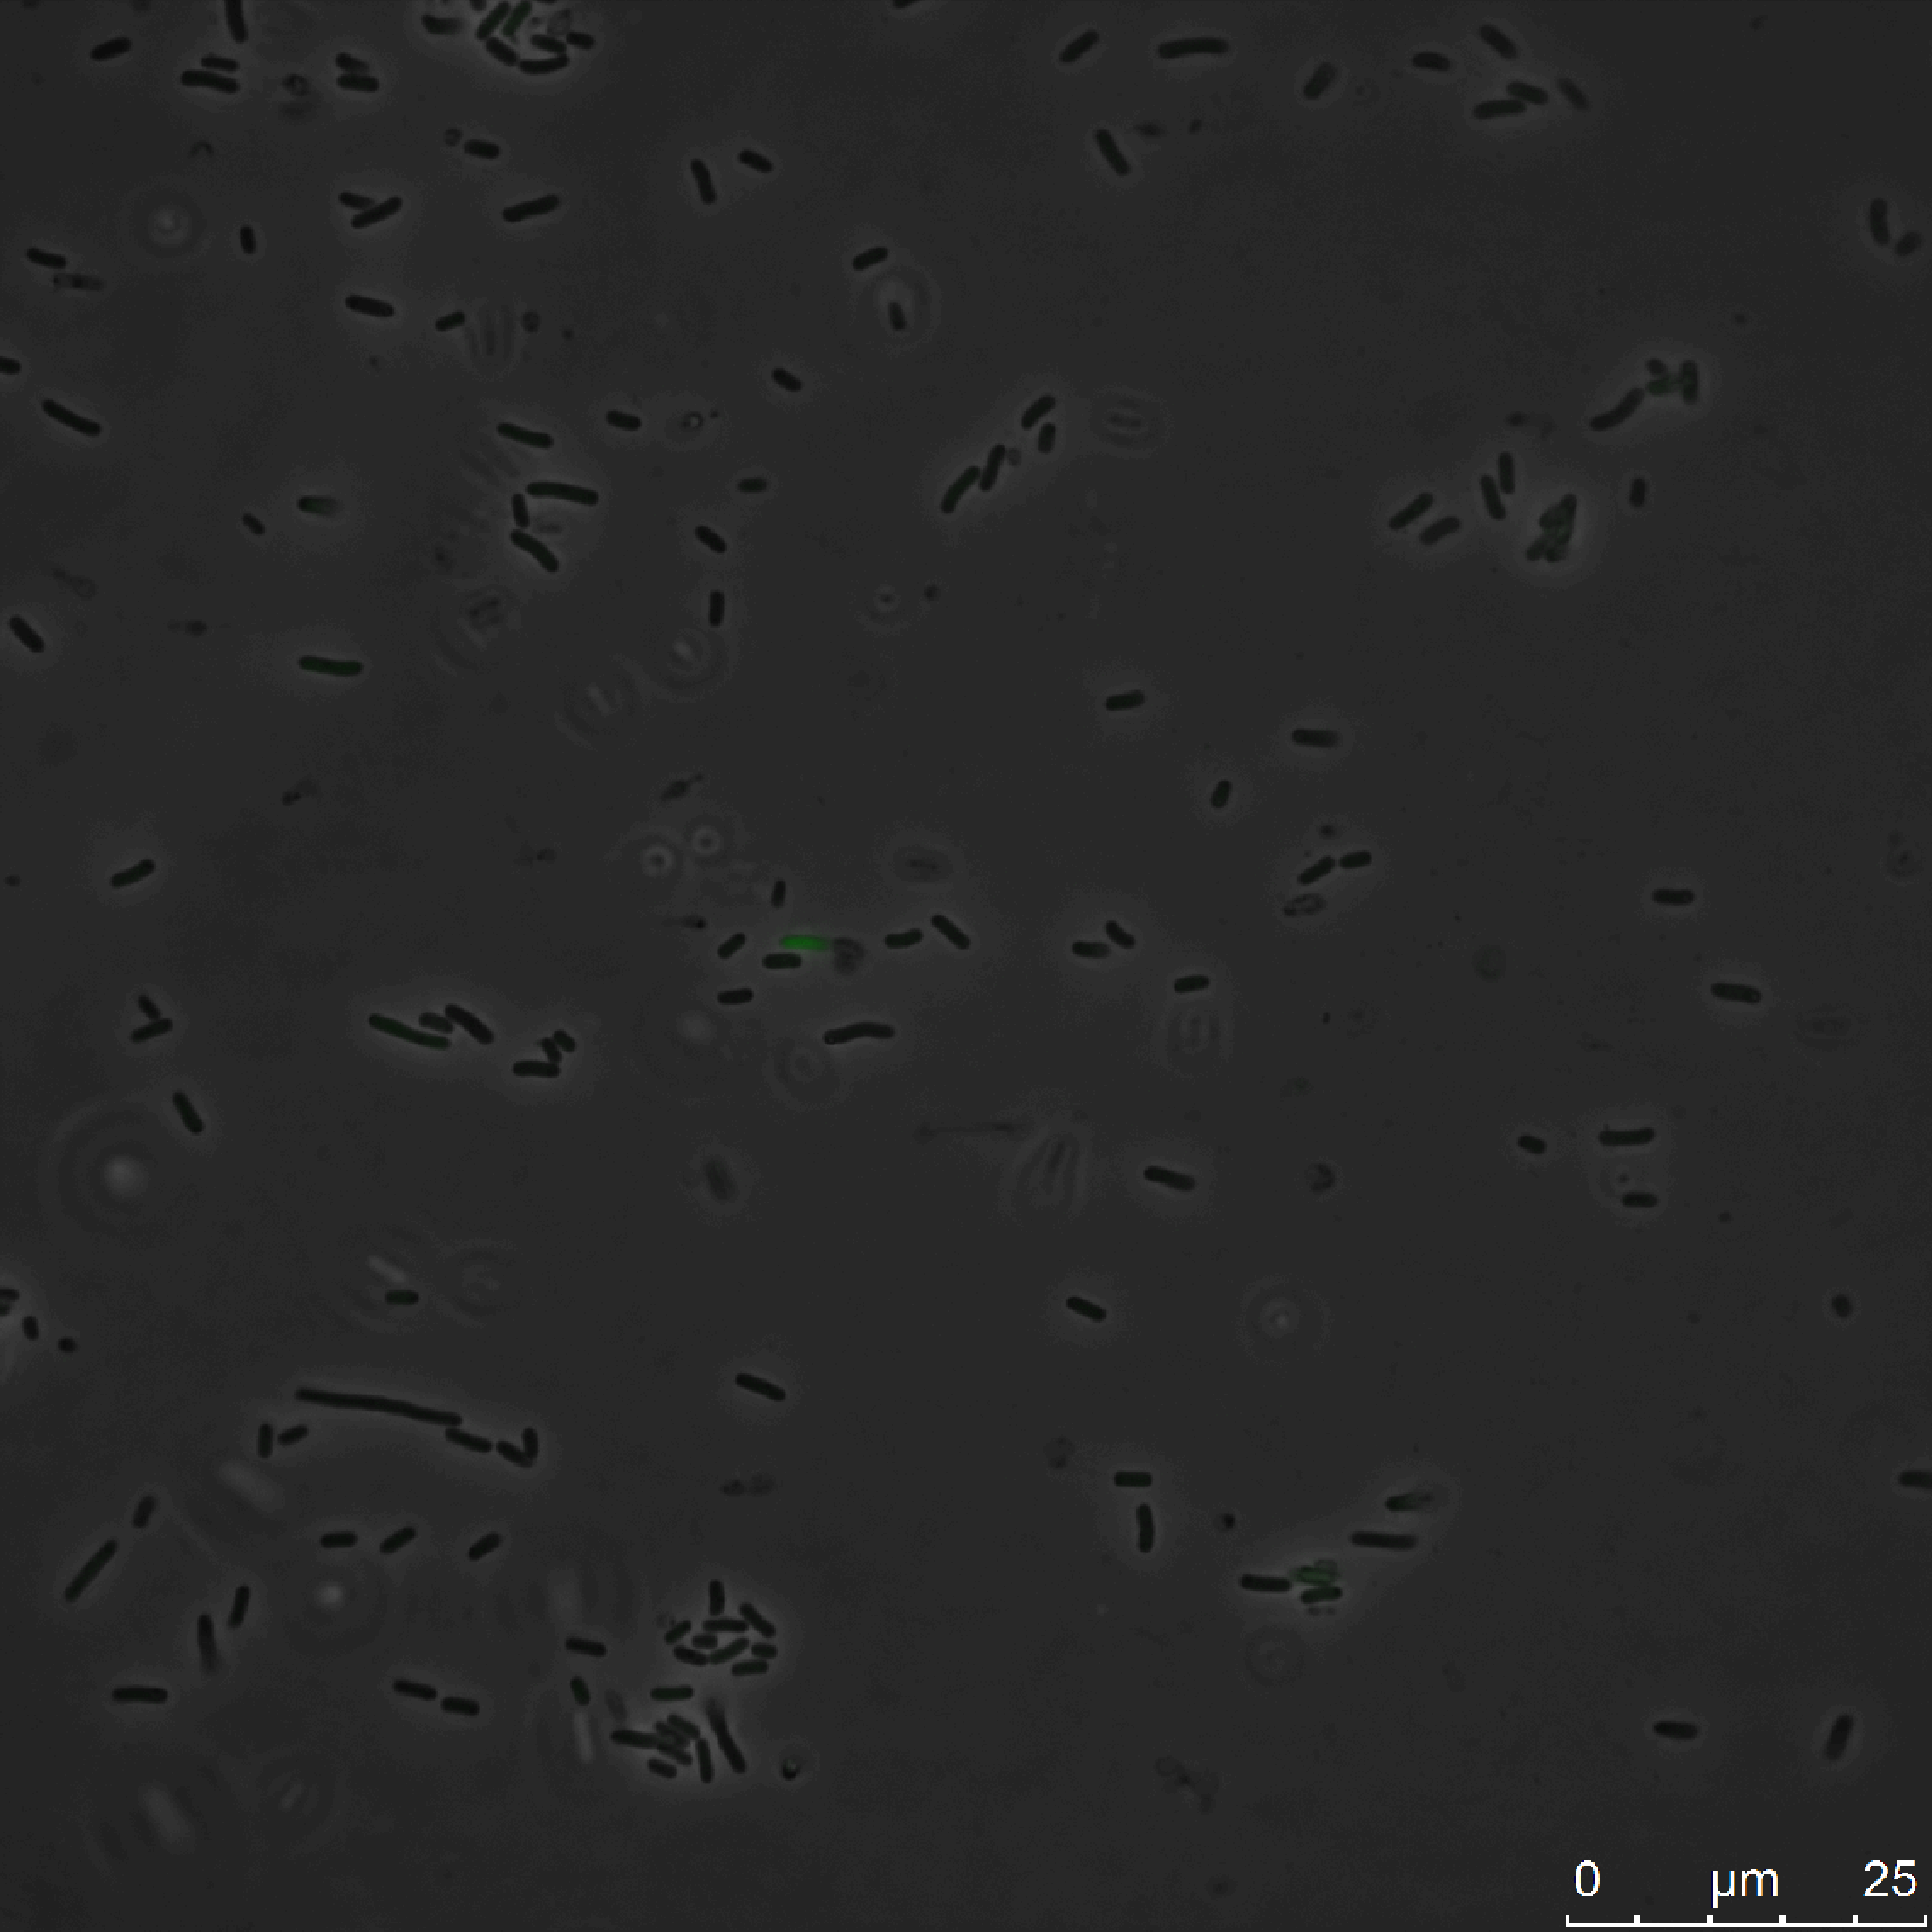
\includegraphics{TT01U1_24HR_4_GREEN.pdf} &%
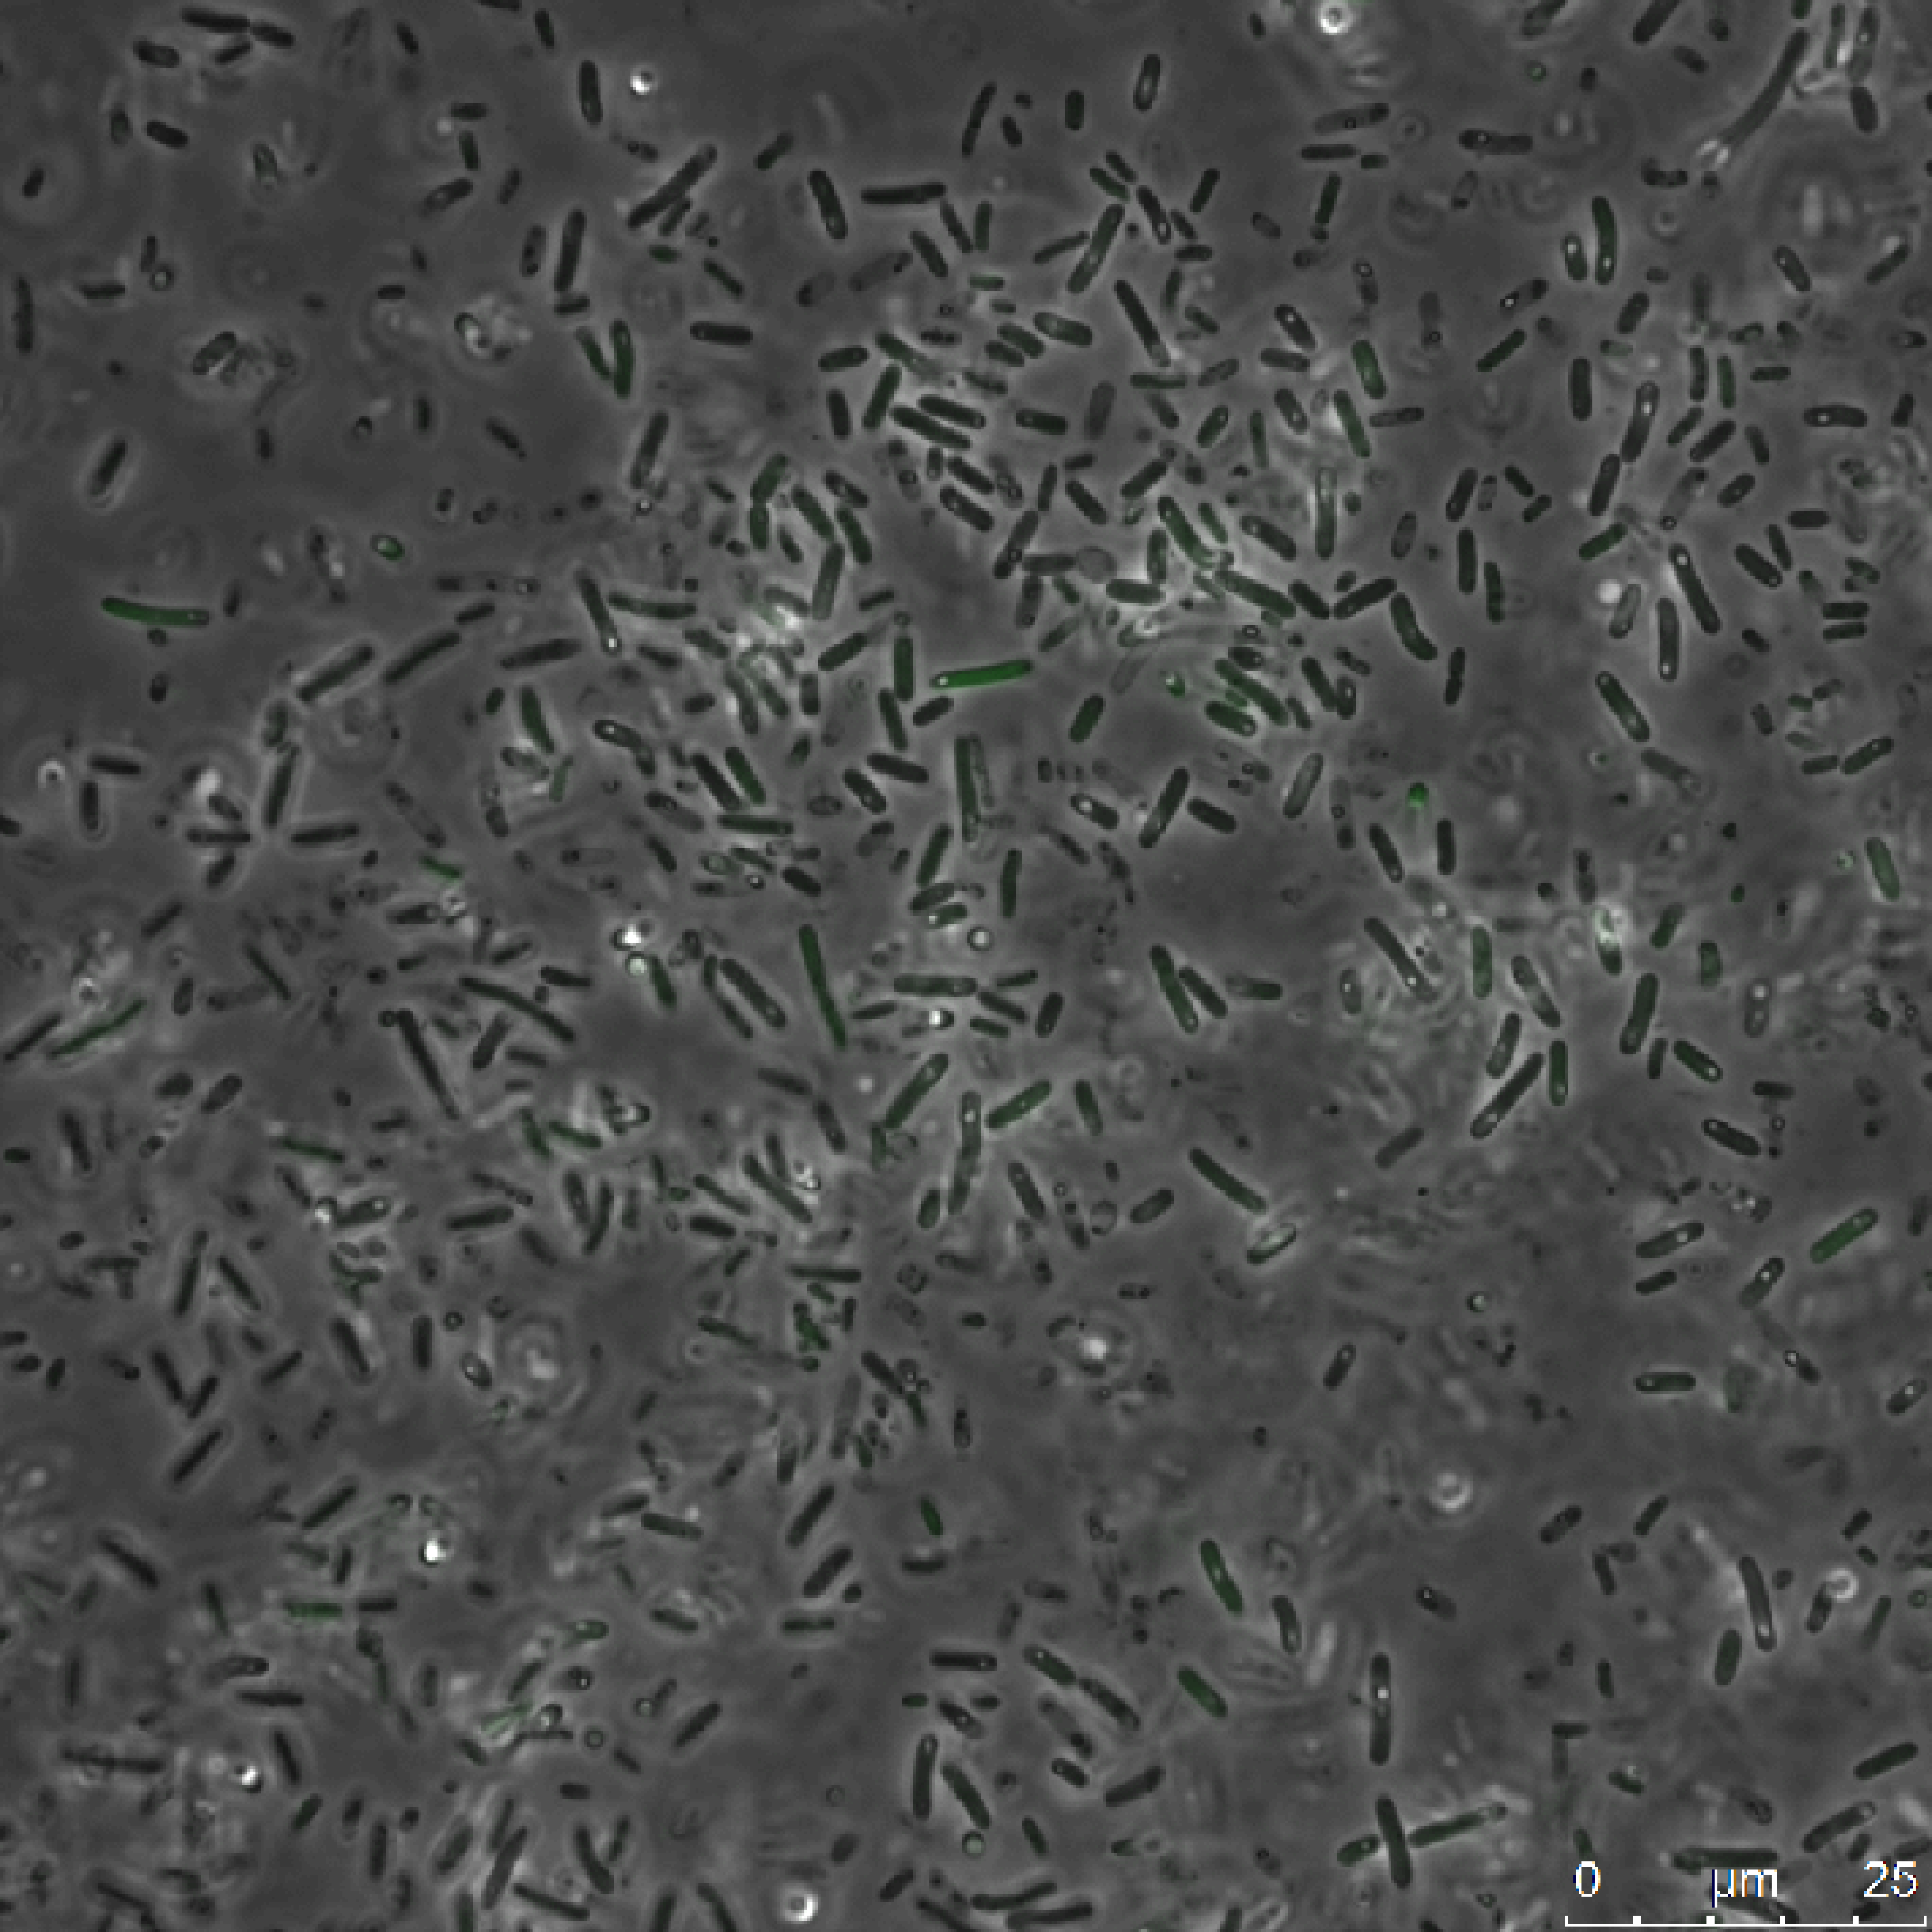
\includegraphics{TT01U1_72HR_5_GREEN.pdf} \\
 - & - &  ++ & ++ \\[1ex]

\end{tabularx}

\label{RMTT01U1}
\captionsetup{singlelinecheck=off, justification=justified, font=footnotesize, aboveskip=20pt}
\caption[Reporter microscopy - TT01 Unit 1]{\textsc{\normalsize Reporter microscopy for the \emph{P. luminescens} TT01 ``Unit 1" promoter.}\vspace{0.1cm} \newline A representative selection of images for 4 time points, for the PVC ``Unit 1" promoter fusion. Quadruplicate images are displayed vertically as representative of the whole slide sample. Key to qualitative fluorescence indication: ``-" - no fluorescence, ``+" - low level fluorescence in isolated cells. ``++" - low level fluorescence in many cells or few brighter cells, ``+++" - intermediate to high fluorescence in almost all cells, or very bright isolated cells.}
\end{figure}
\endgroup

%%%%%%%%%%%%%%%%%%%%%%%%%%%%%%%%%%%%%%%%%%%%%%%%%%%%%%%%%%%%%%%%%%%%

\begingroup
\renewcommand{\arraystretch}{0.8}%
\setlength{\tabcolsep}{0.3pt}
\begin{figure}[p]
\setkeys{Gin}{width=\linewidth}
\Huge
\begin{tabularx}{\textwidth}{CCCC}
\multicolumn{4}{p{\linewidth}}{\large \centering \textbf{\emph{P. asymbiotica} PB68.1 (``THAI") PVC ``Unit 1"}} \\
\hiderowcolors
& & & \\[-1.5ex]
\Large 2 Hours &\Large 5 Hours &\Large 24 Hours &\Large 72 Hours \\[1ex]

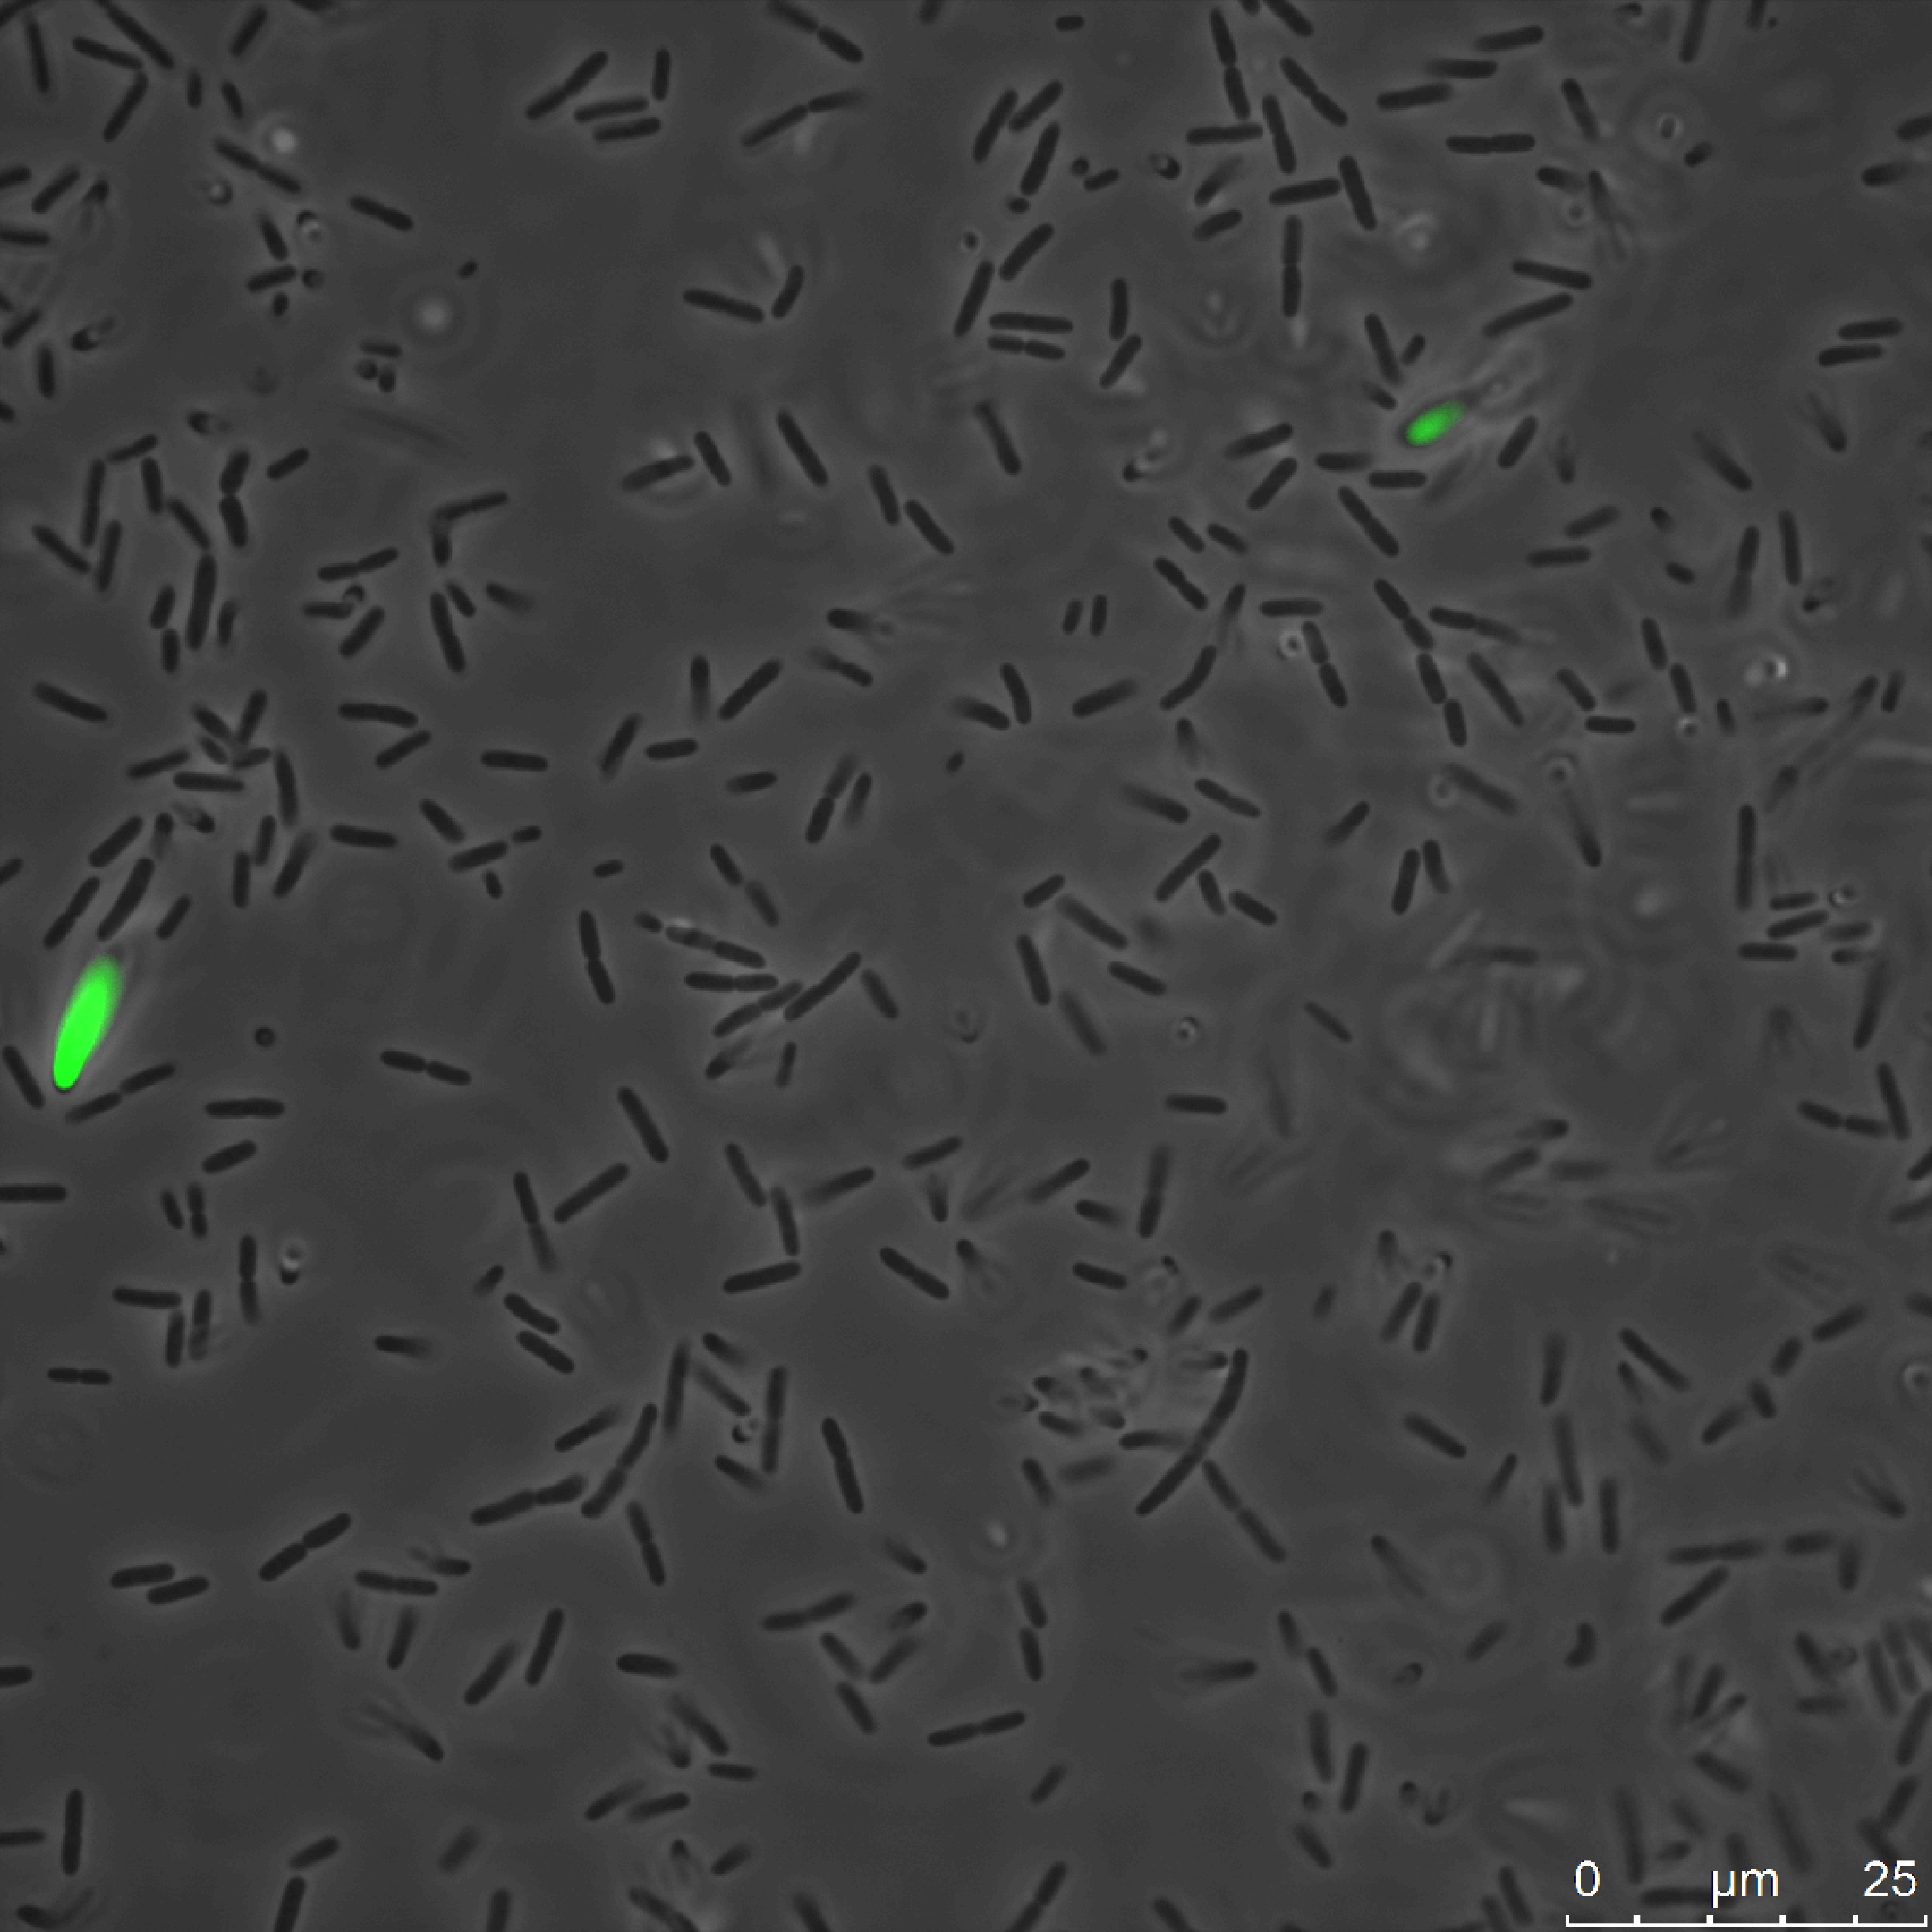
\includegraphics{THAIU1_1_GREEN.pdf} &%
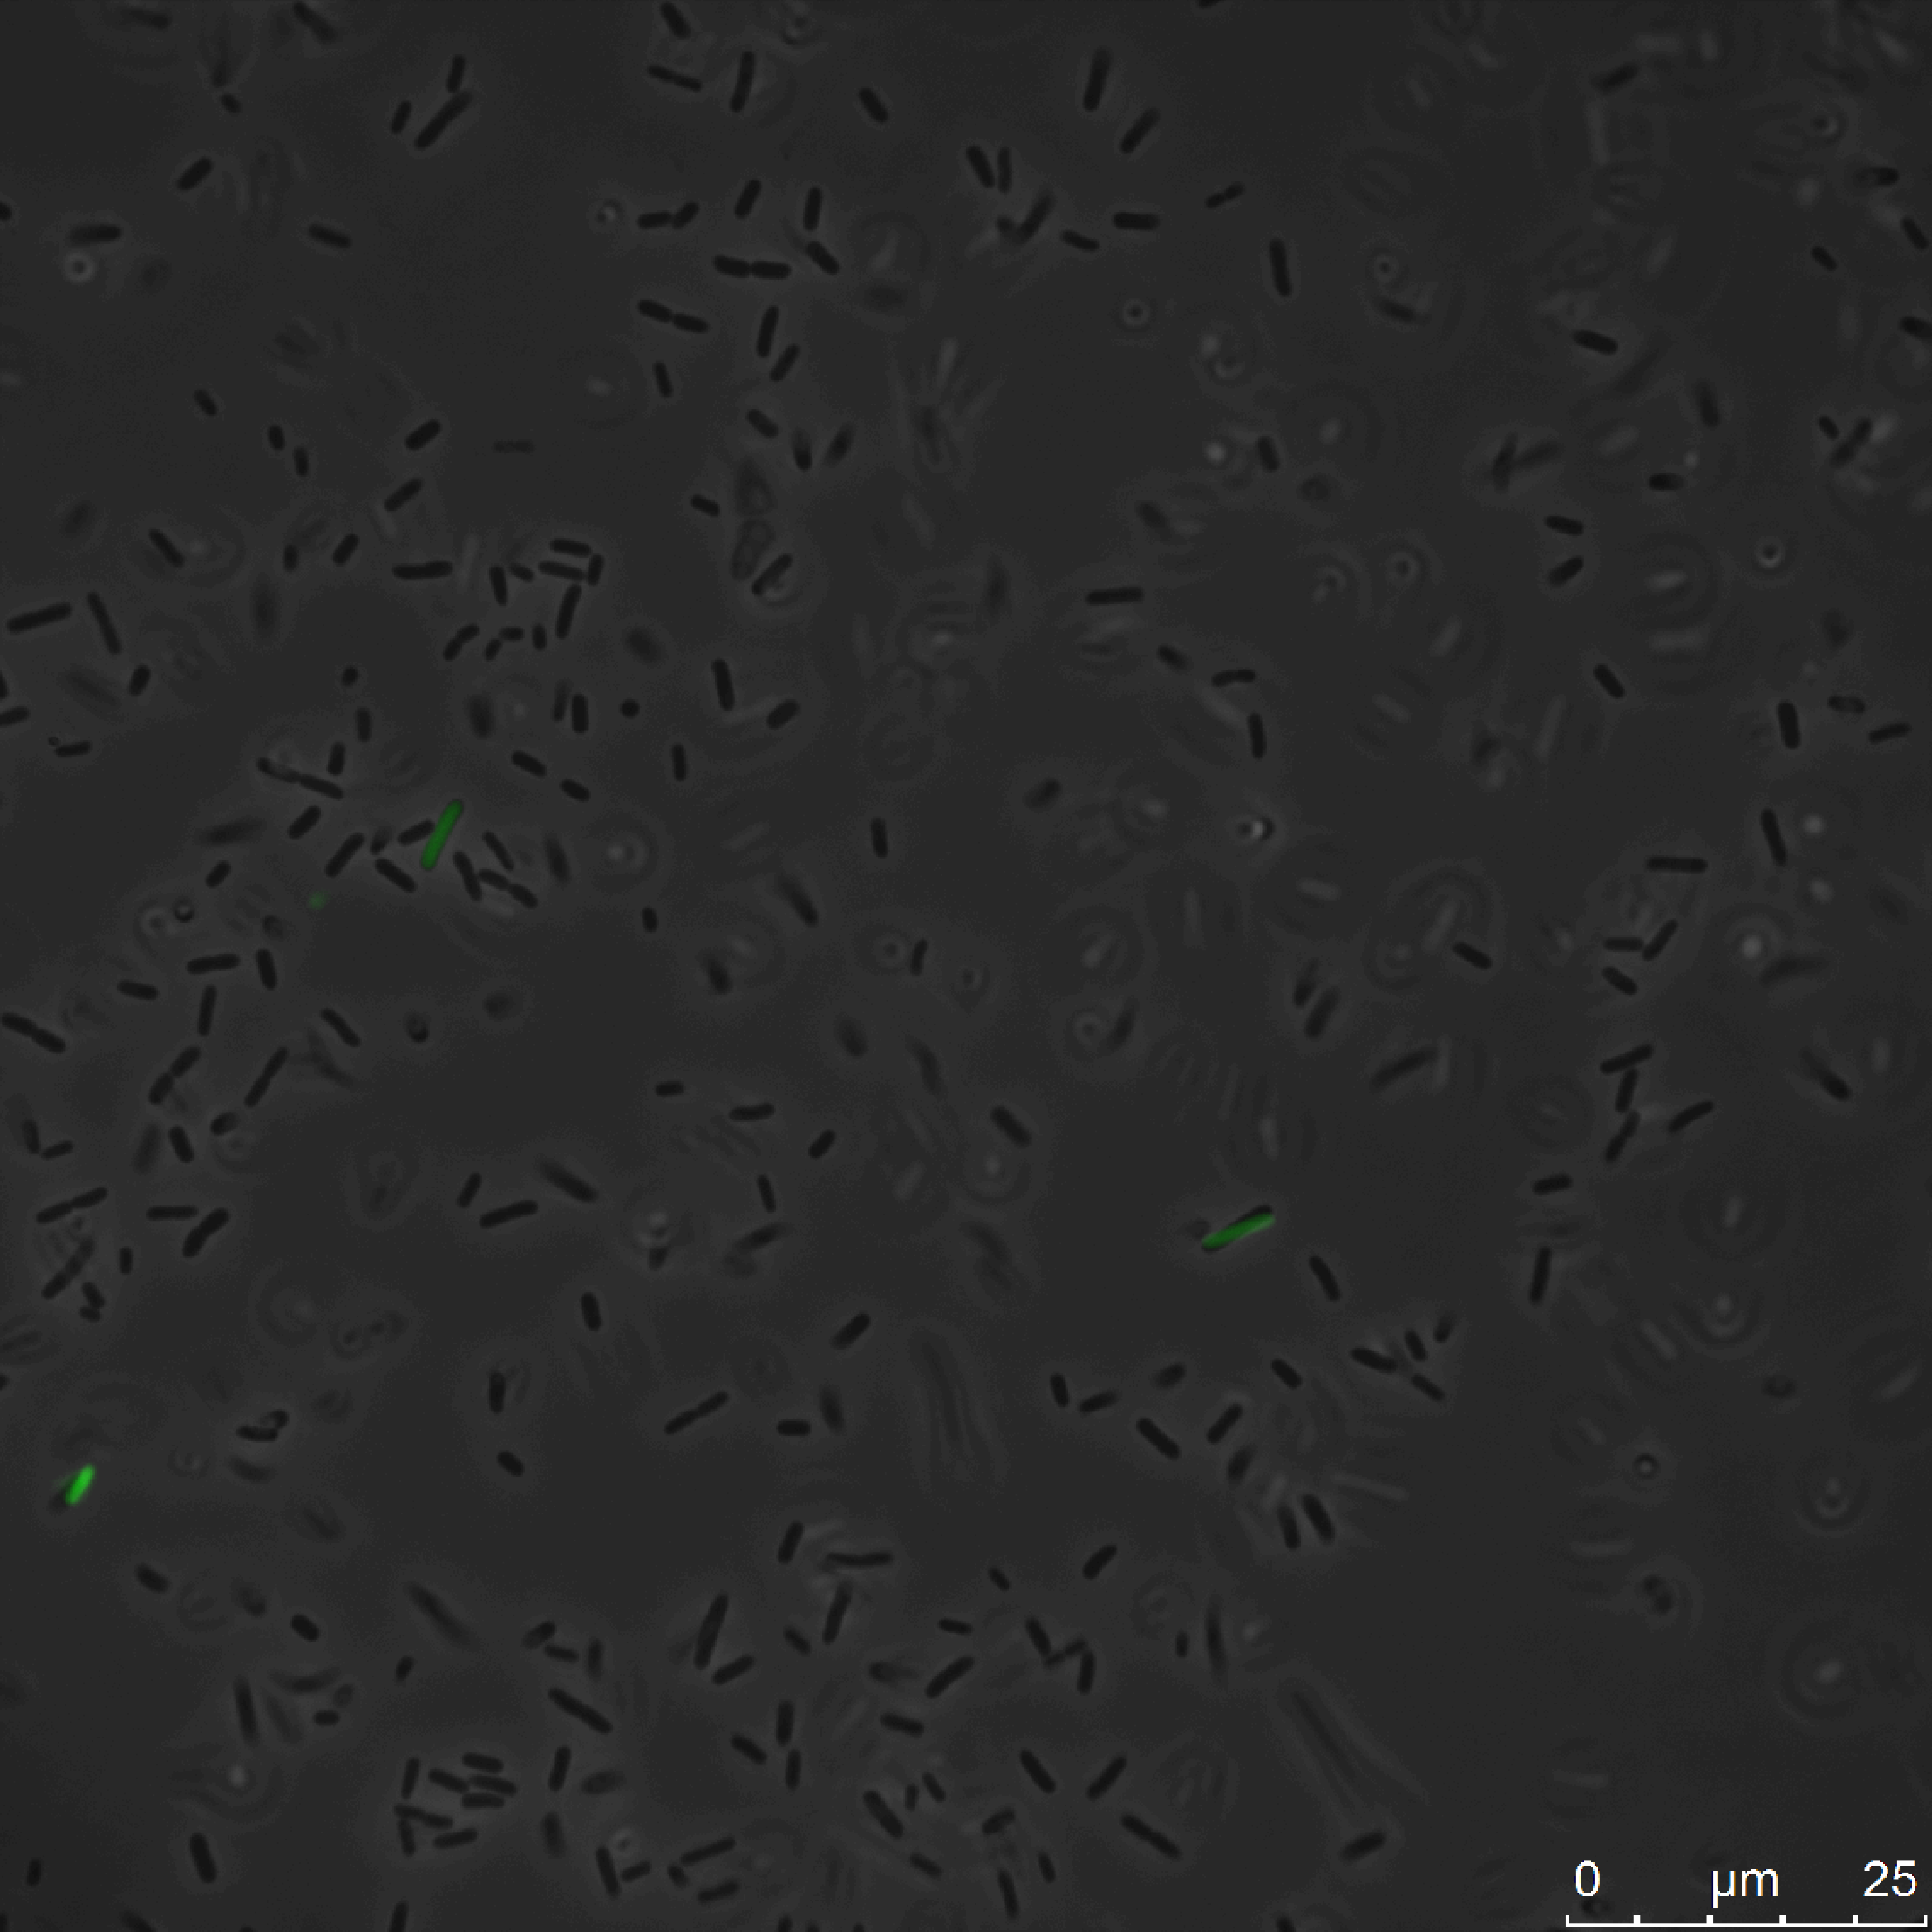
\includegraphics{THAIU1_5HR_5_GREEN.pdf} &%
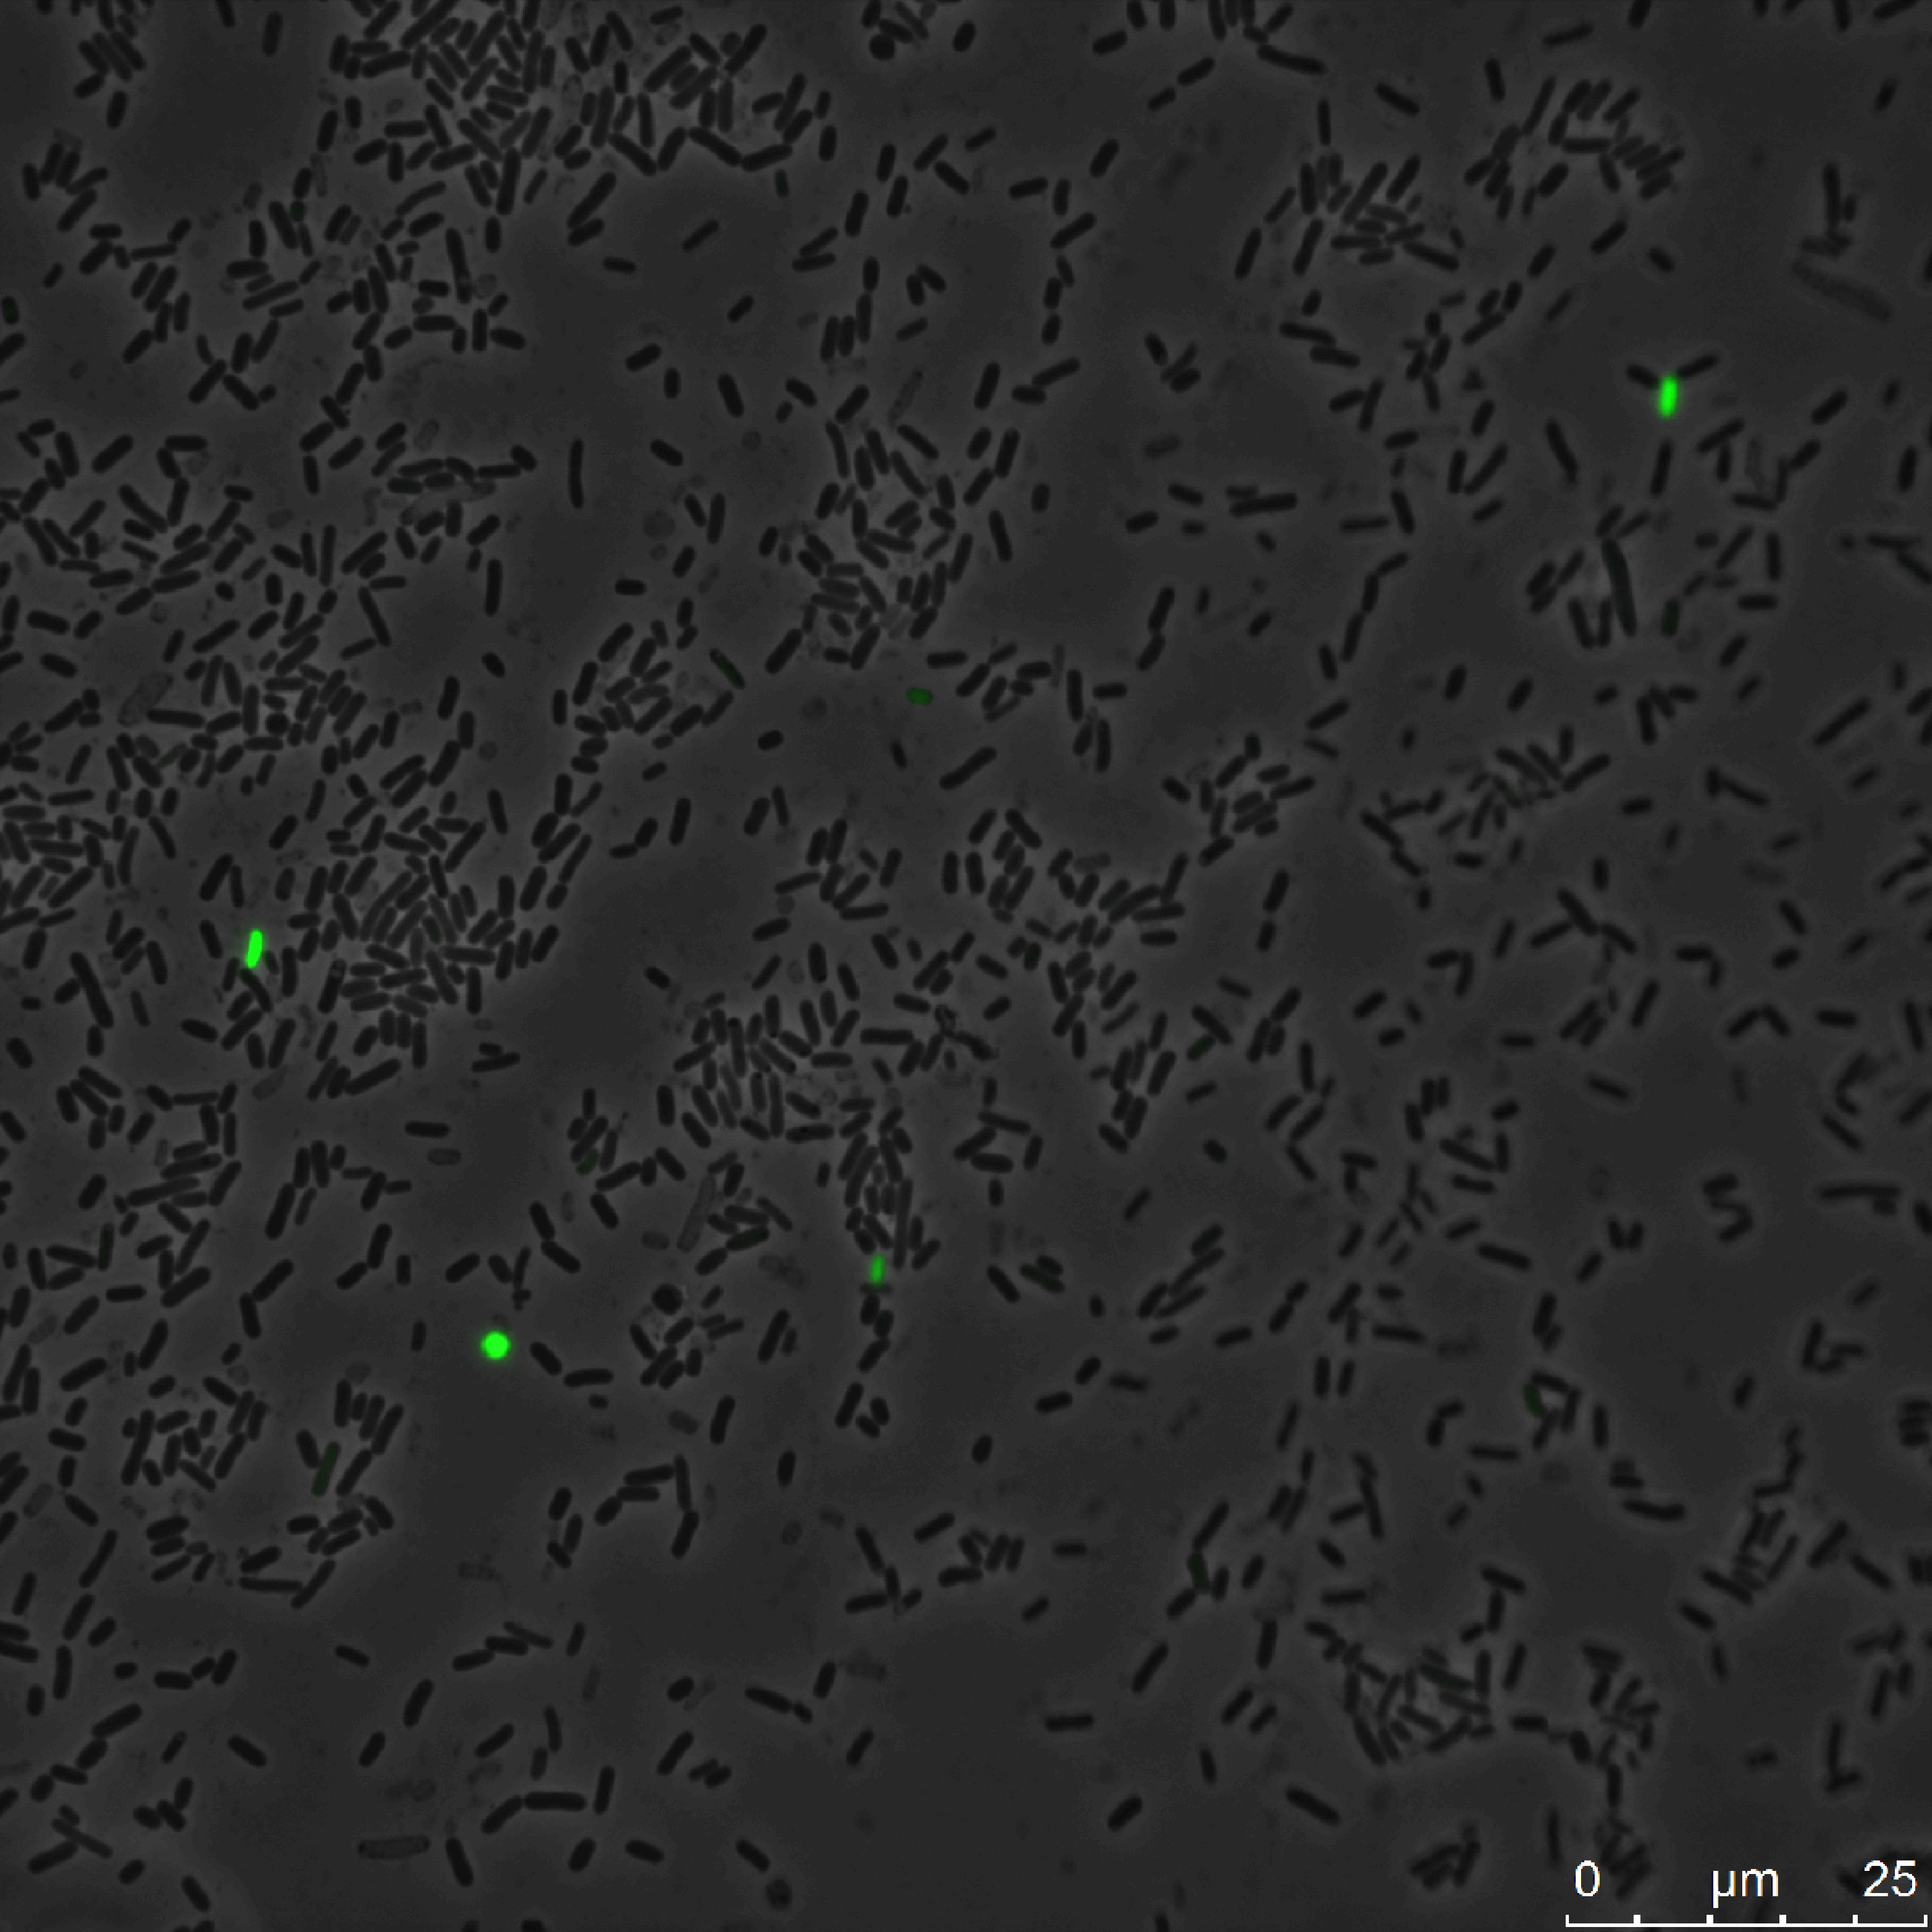
\includegraphics{THAIU1_24HR_1_GREEN.pdf} &%
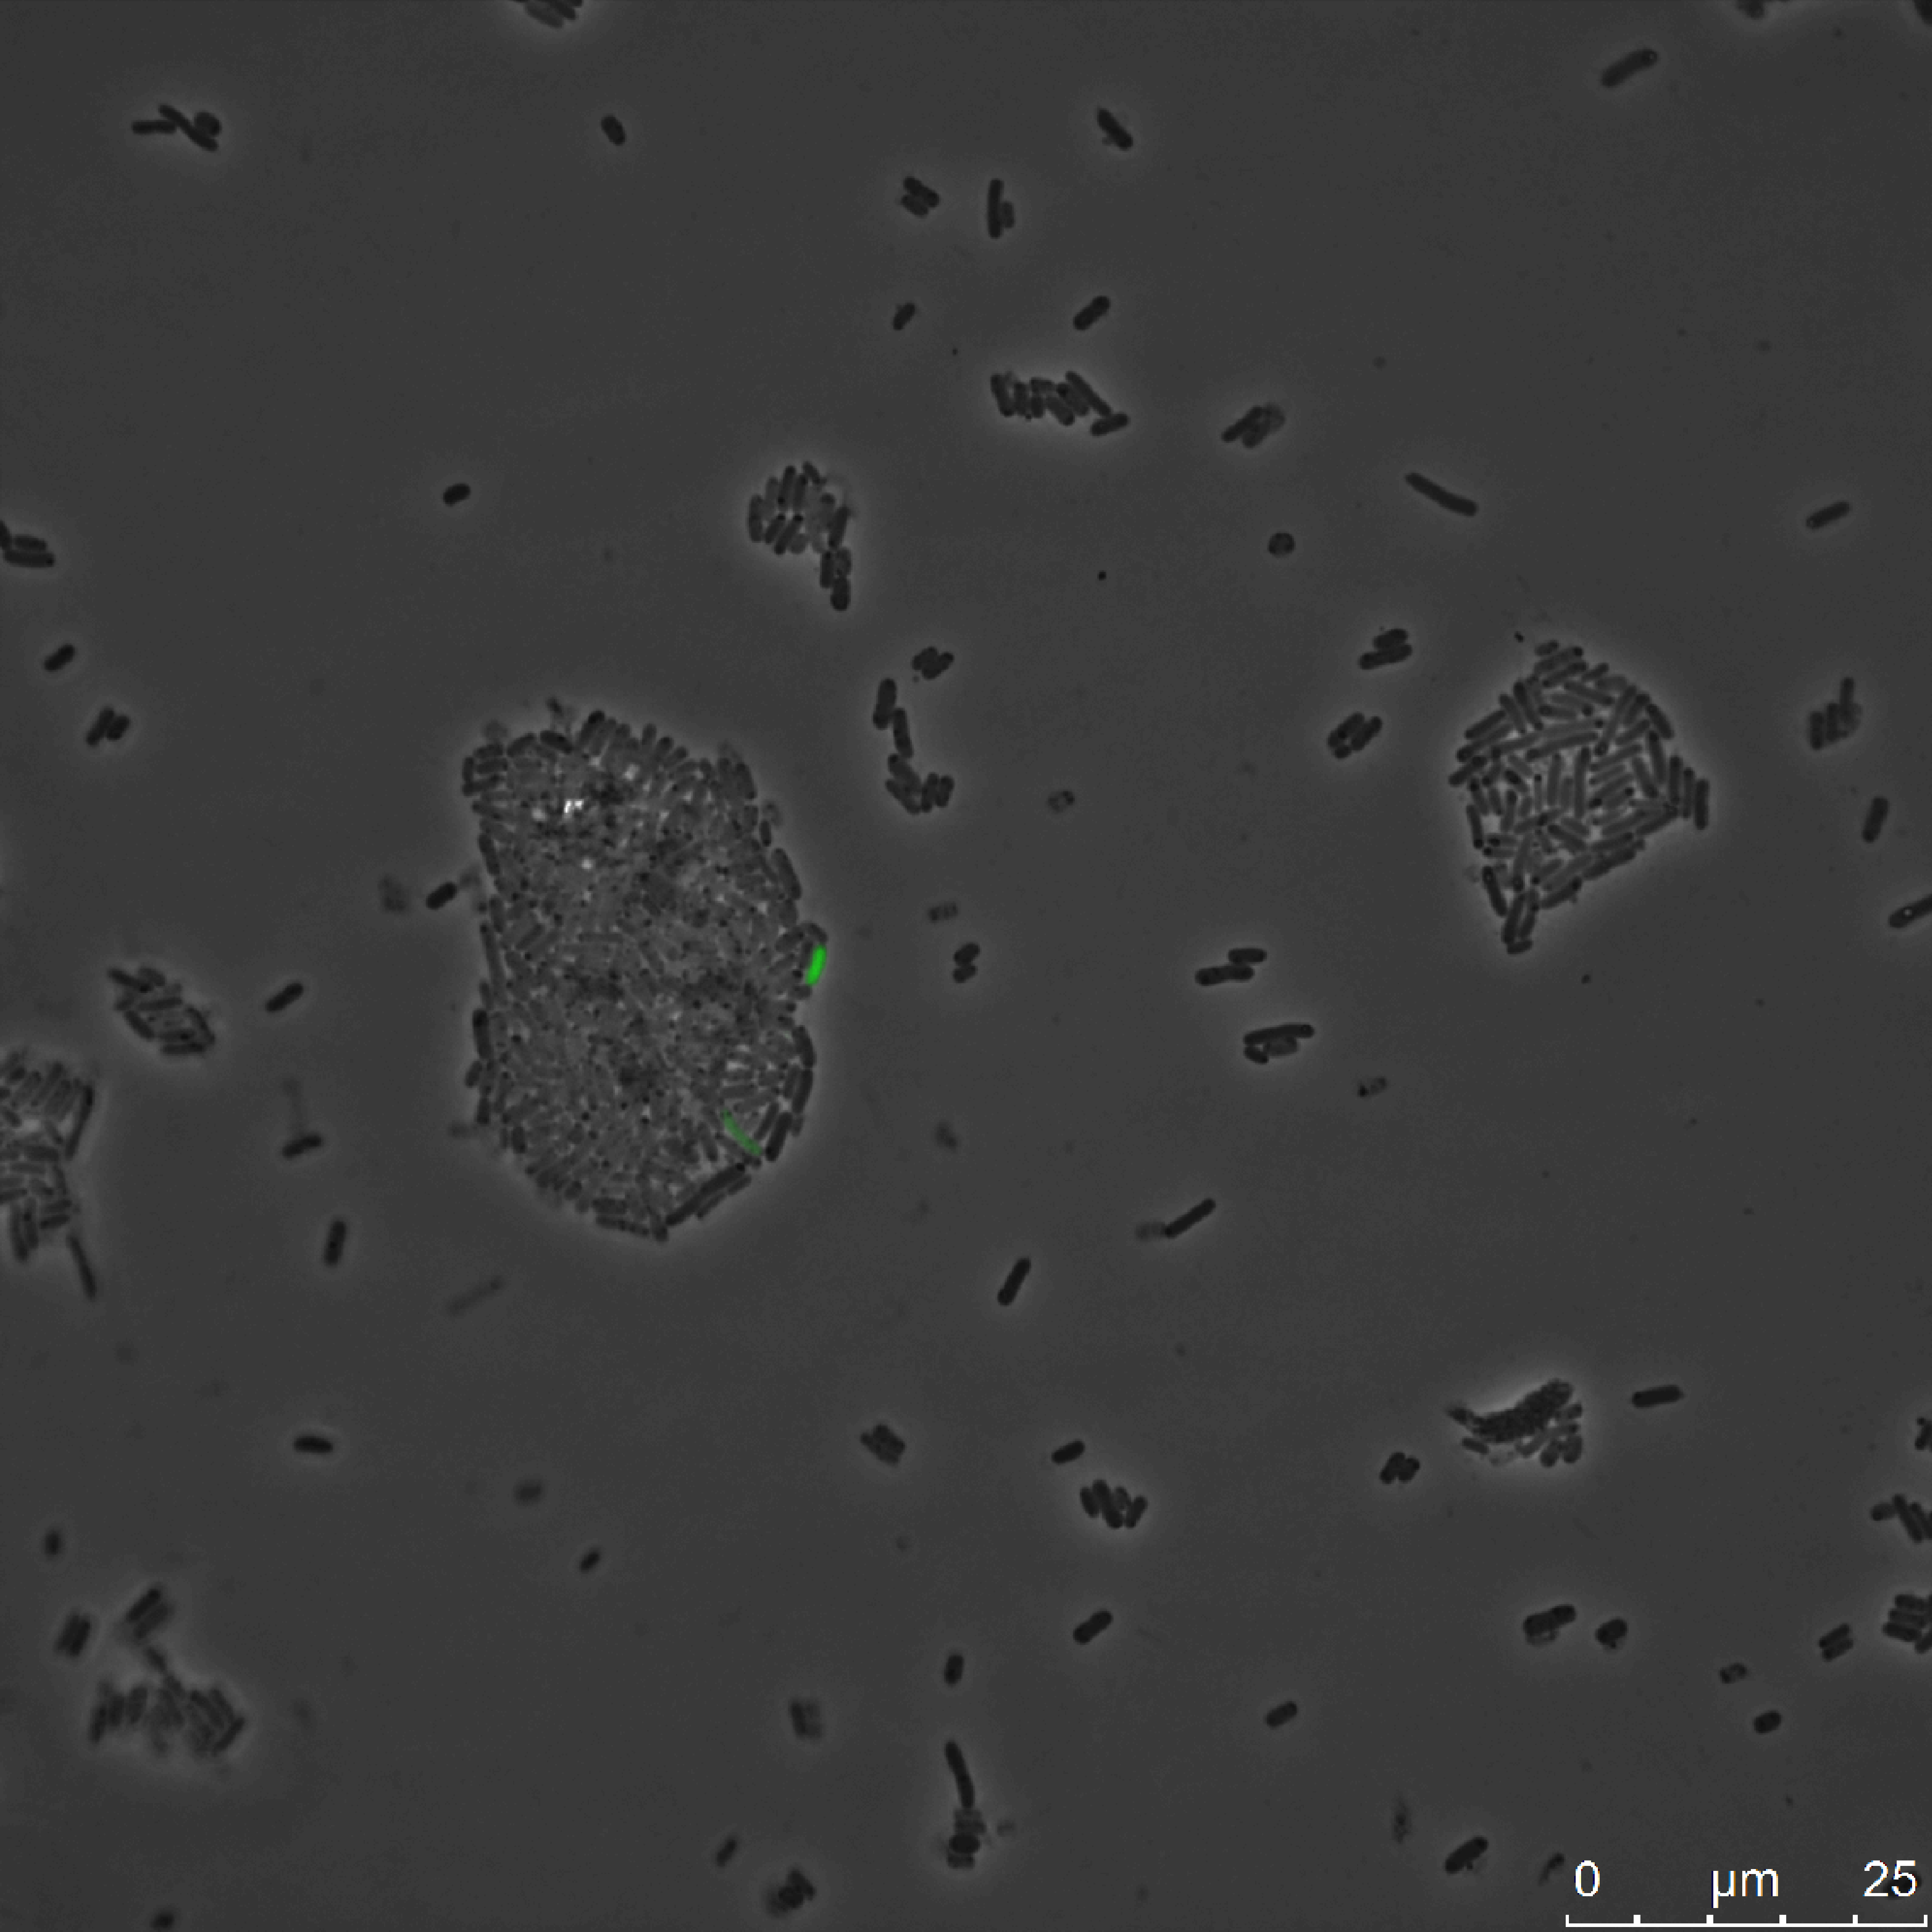
\includegraphics{THAIU1_72HR_1_GREEN.pdf} \\[-0.5ex]

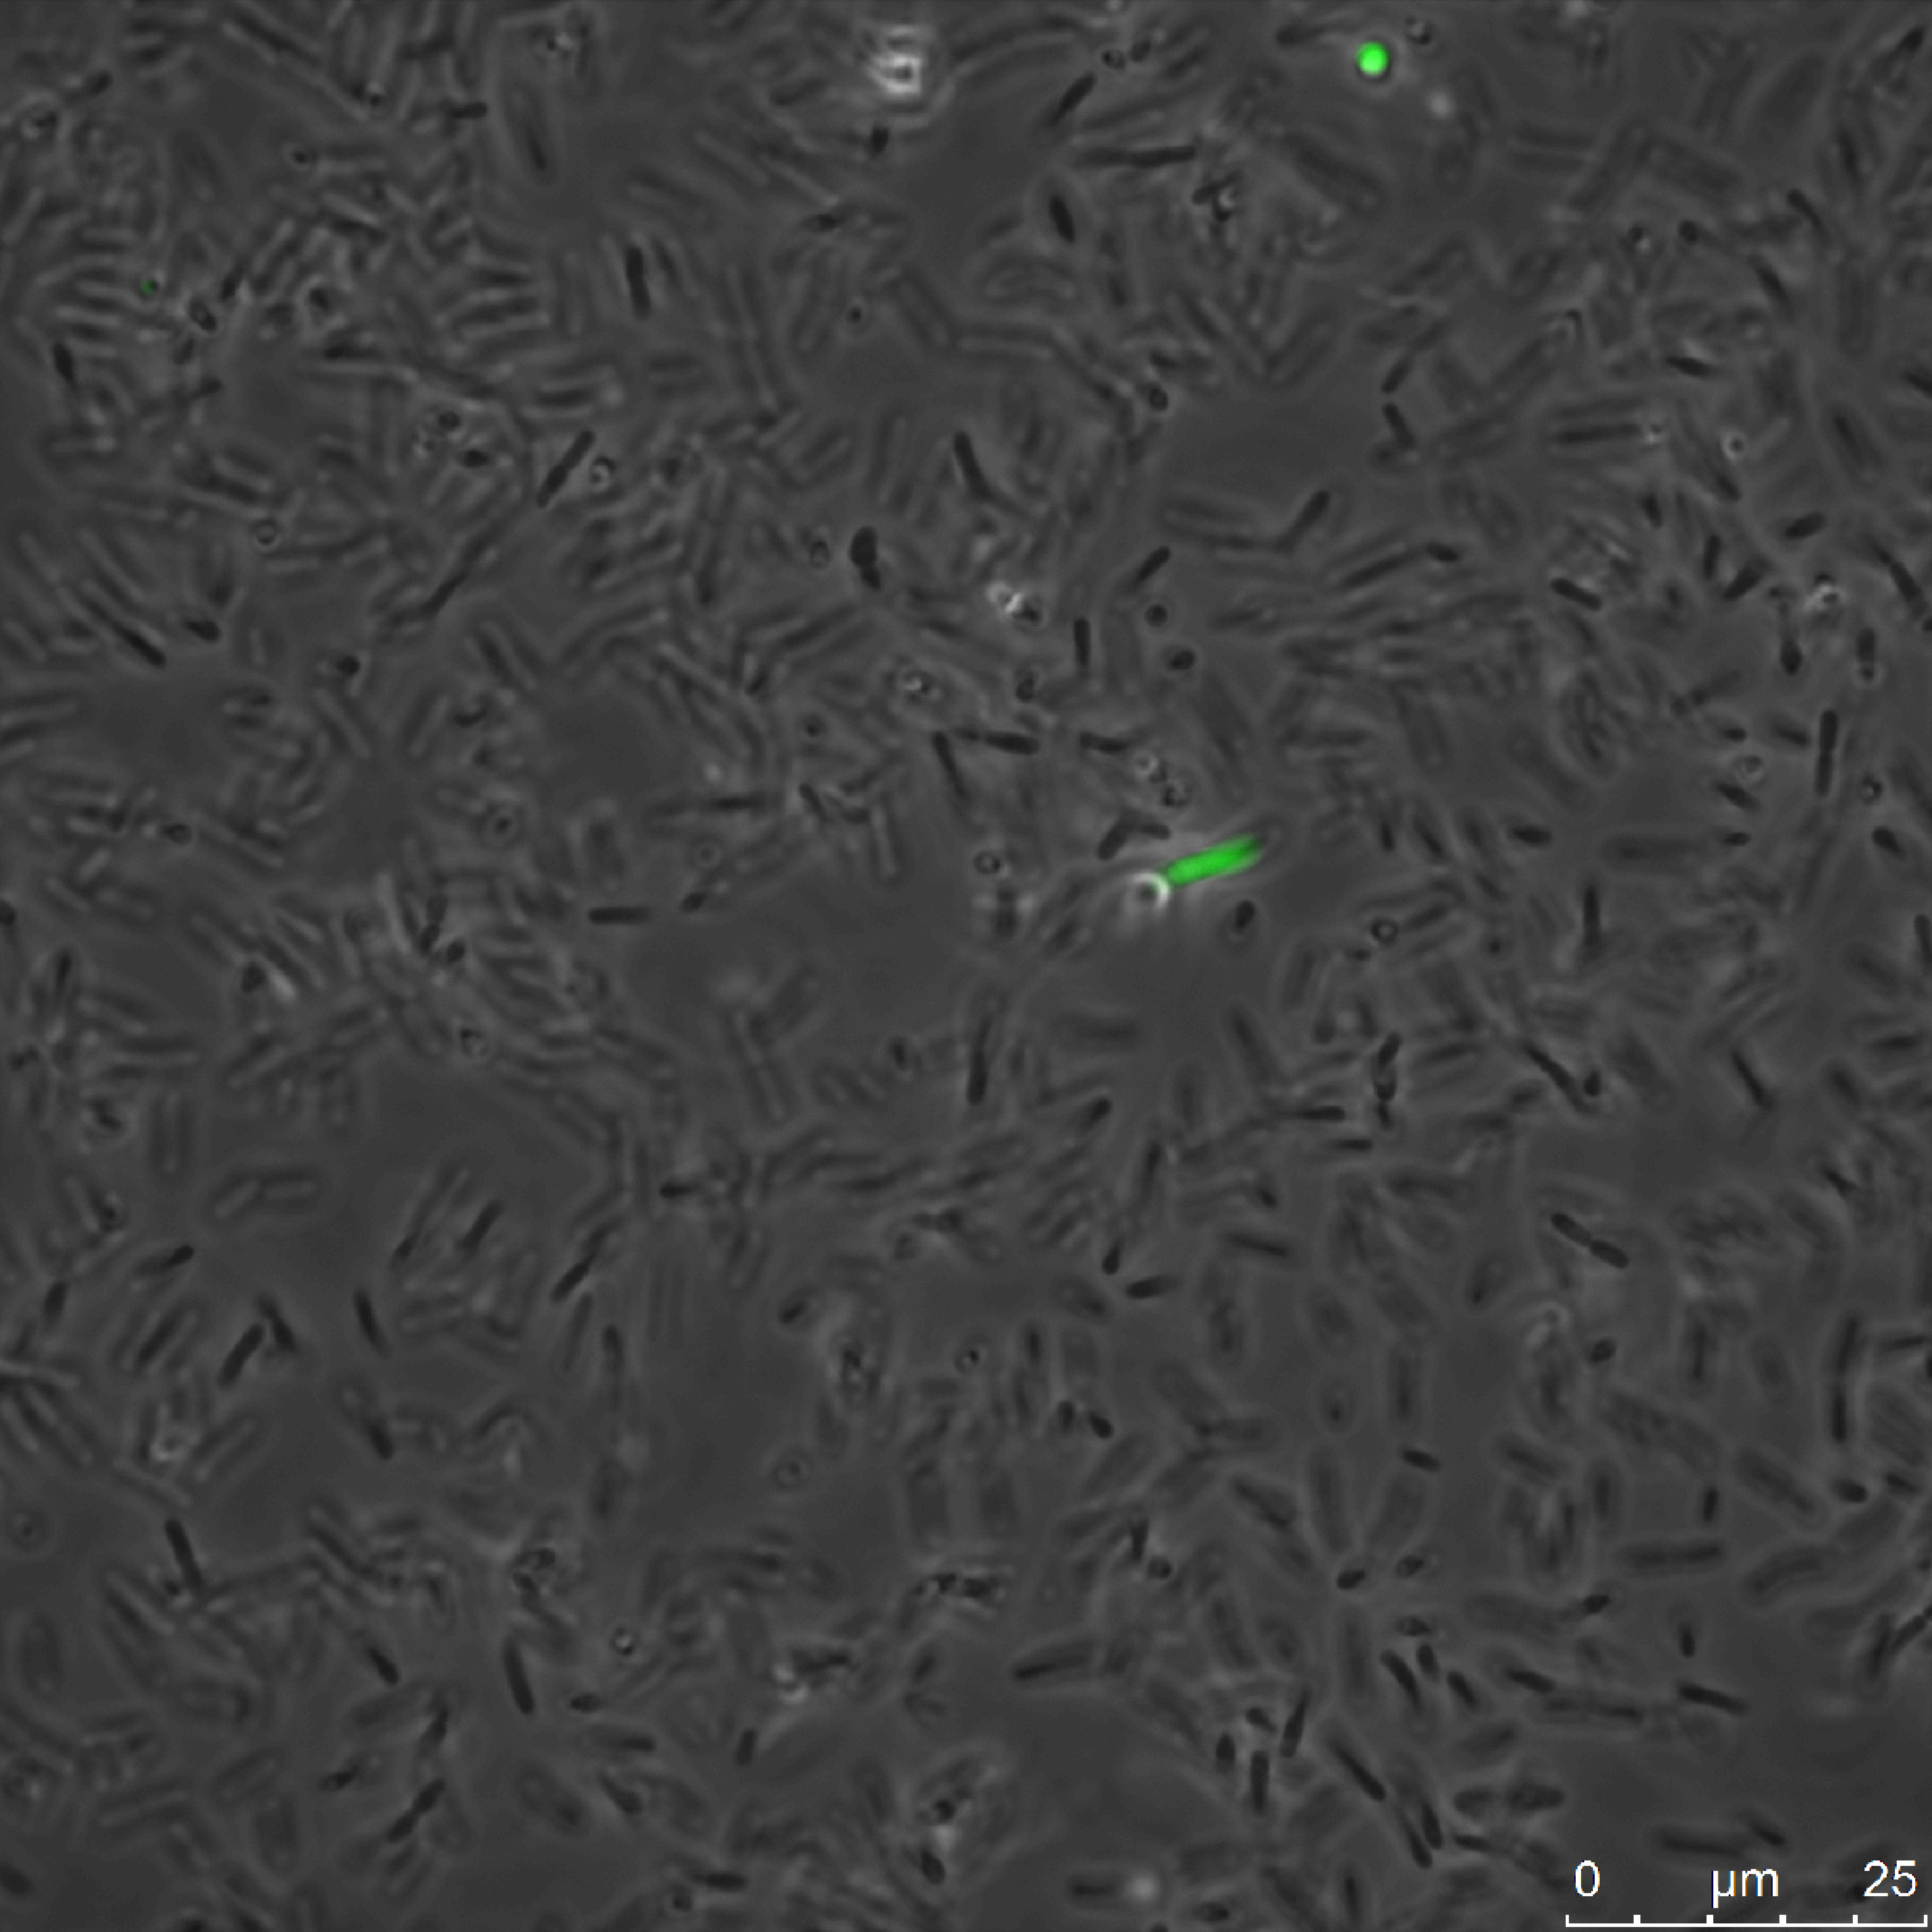
\includegraphics{THAIU1_2_GREEN.pdf} &%
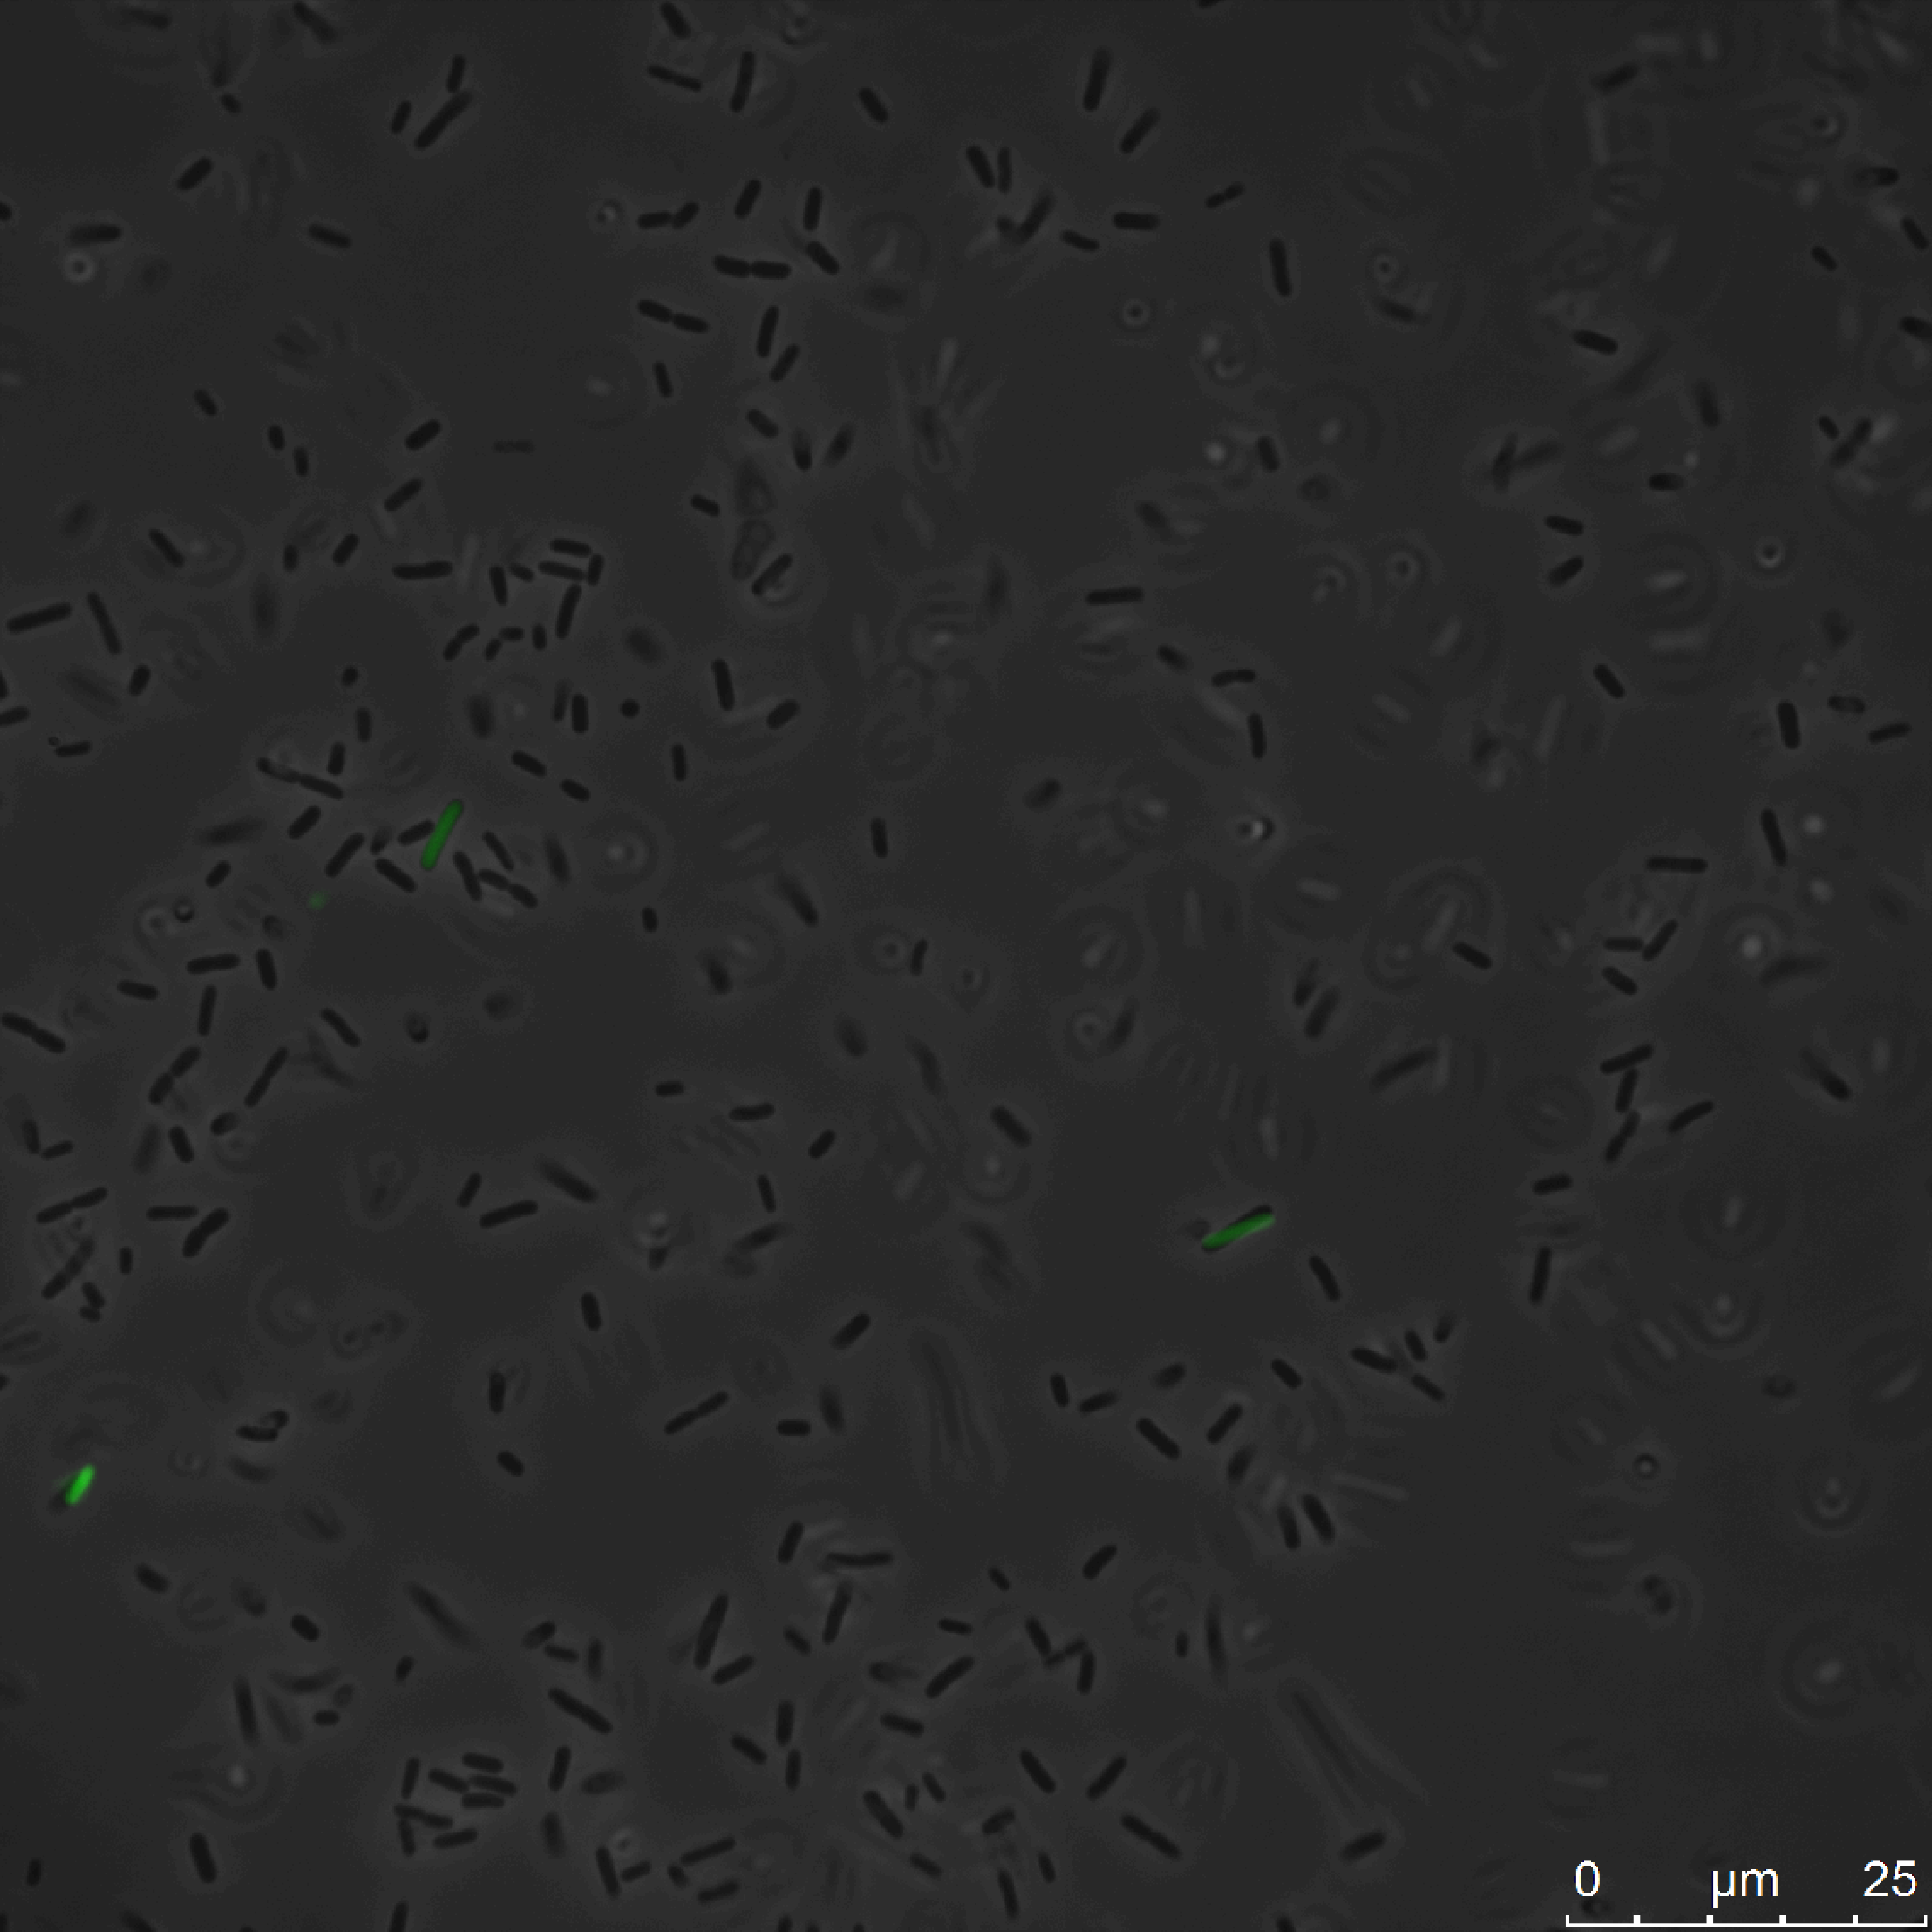
\includegraphics{THAIU1_5HR_5_GREEN.pdf} &%
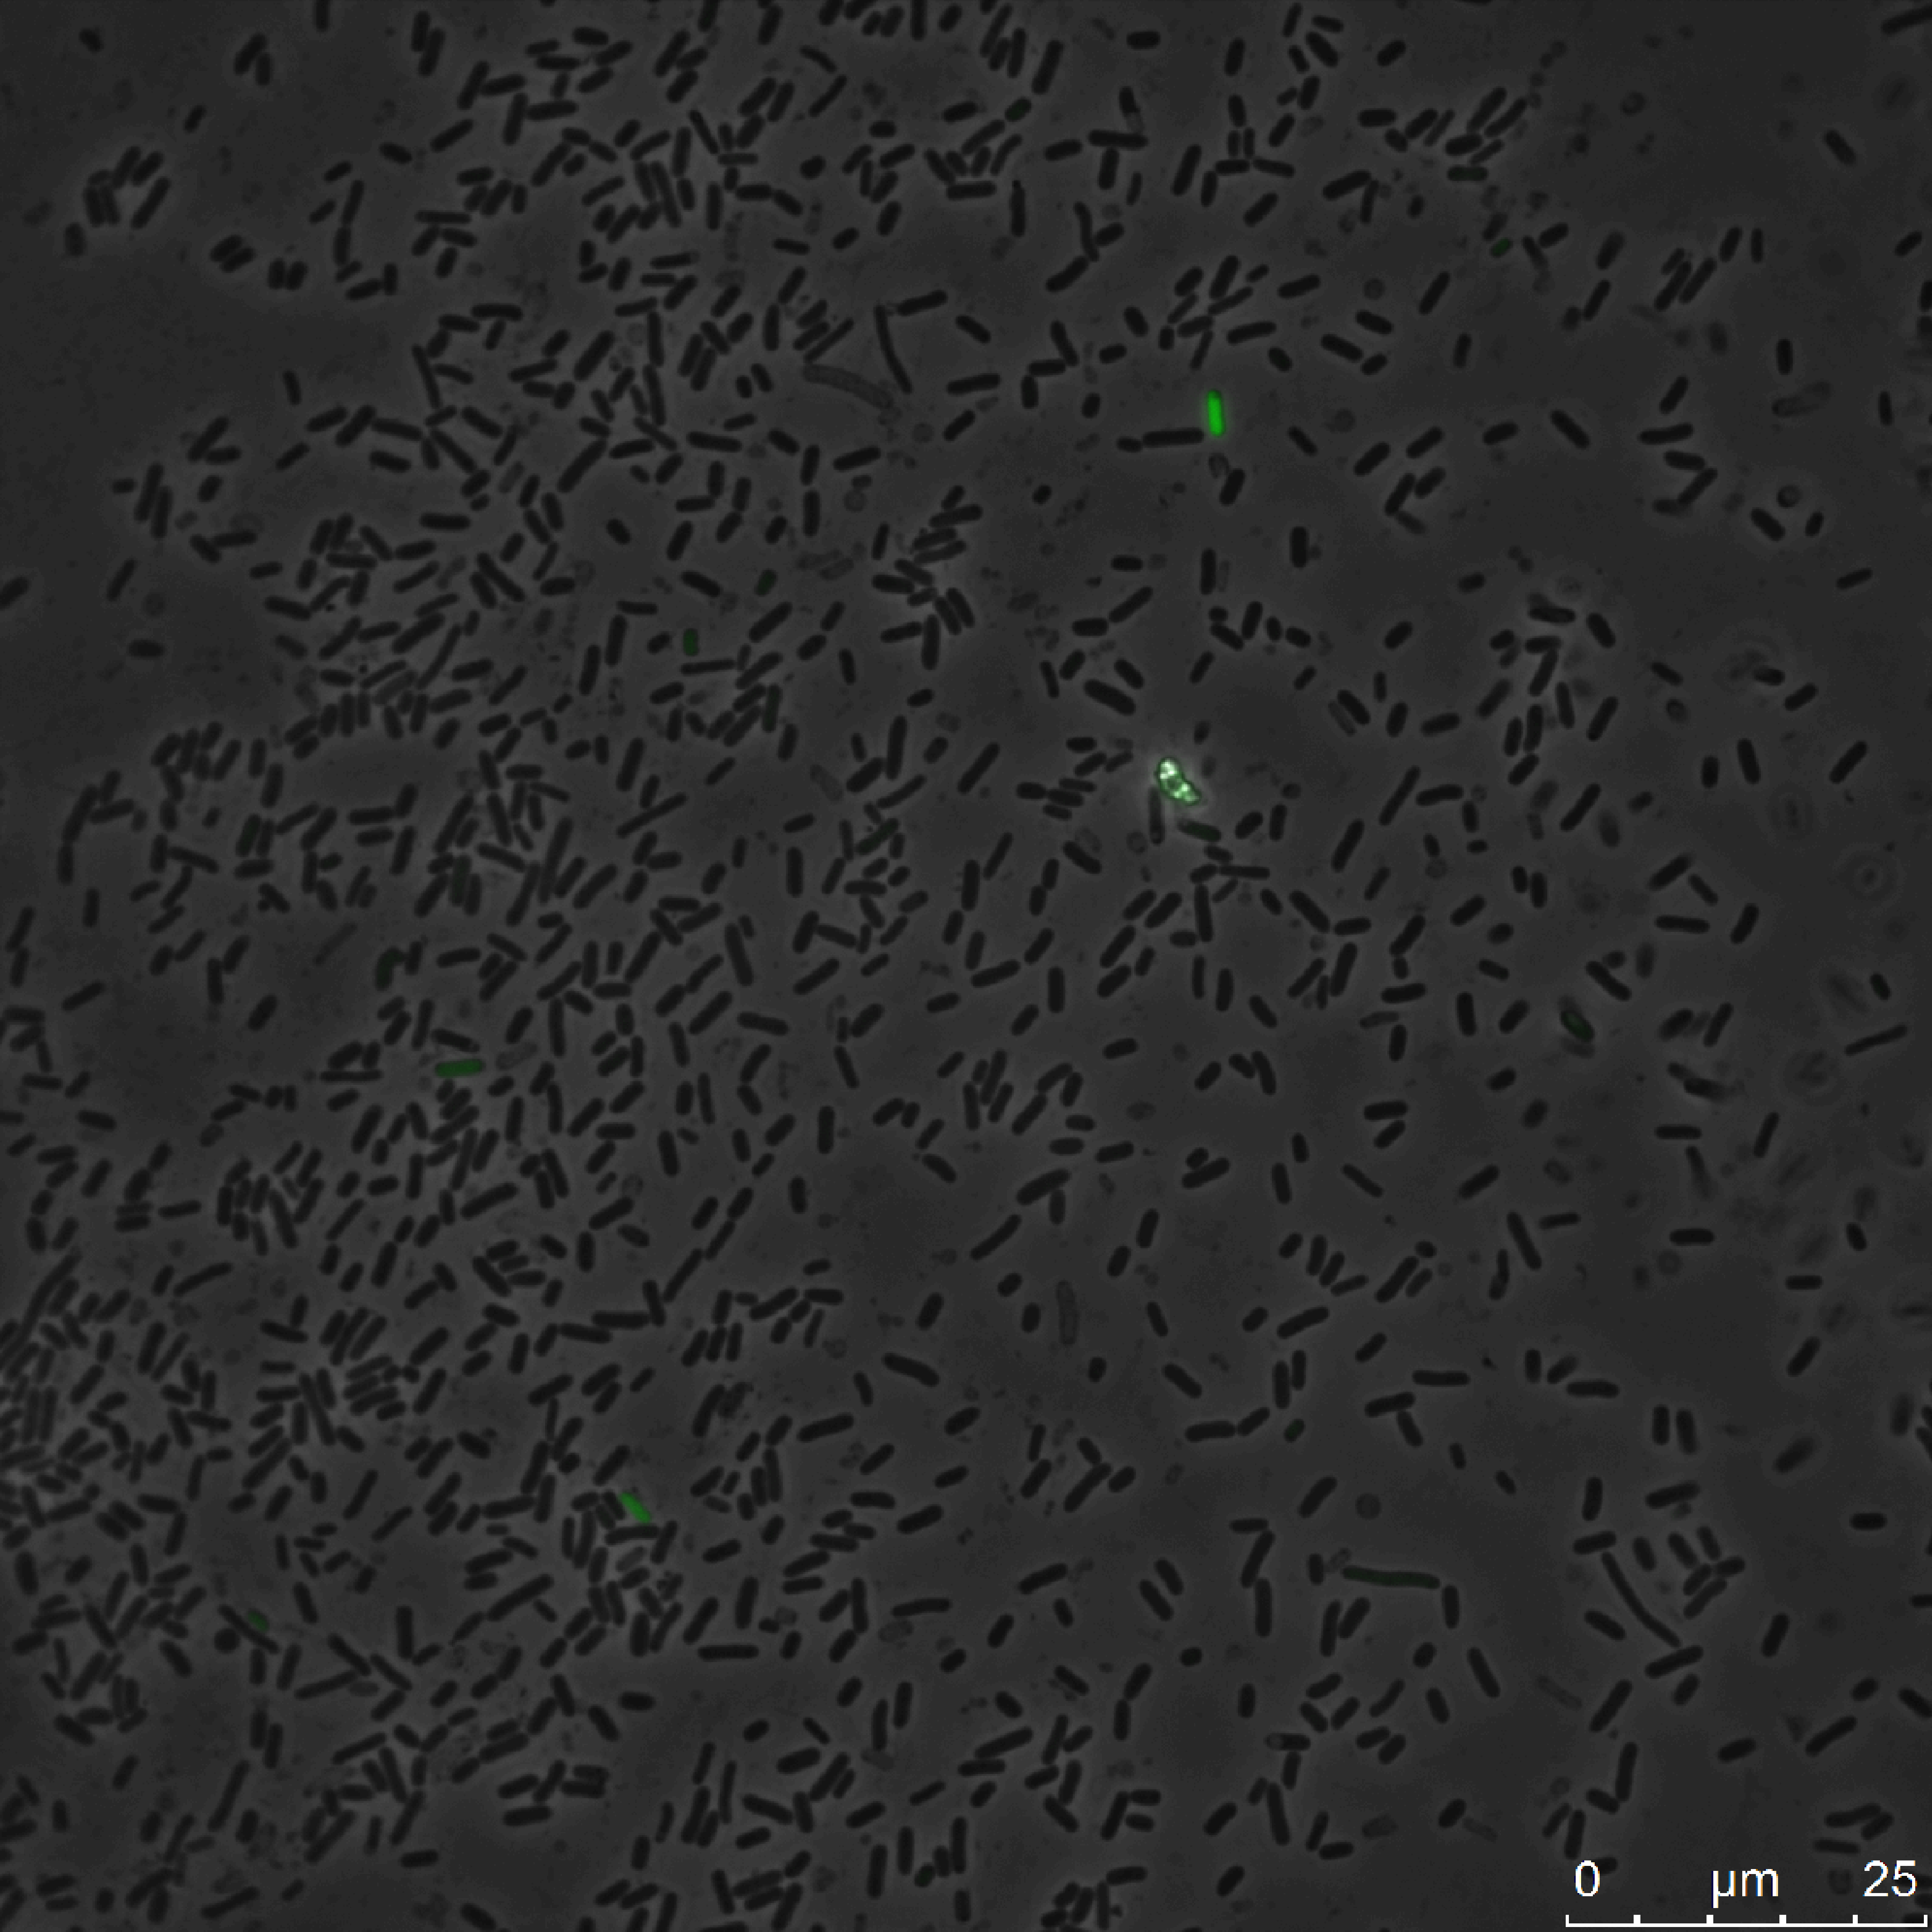
\includegraphics{THAIU1_24HR_2_GREEN.pdf} &%
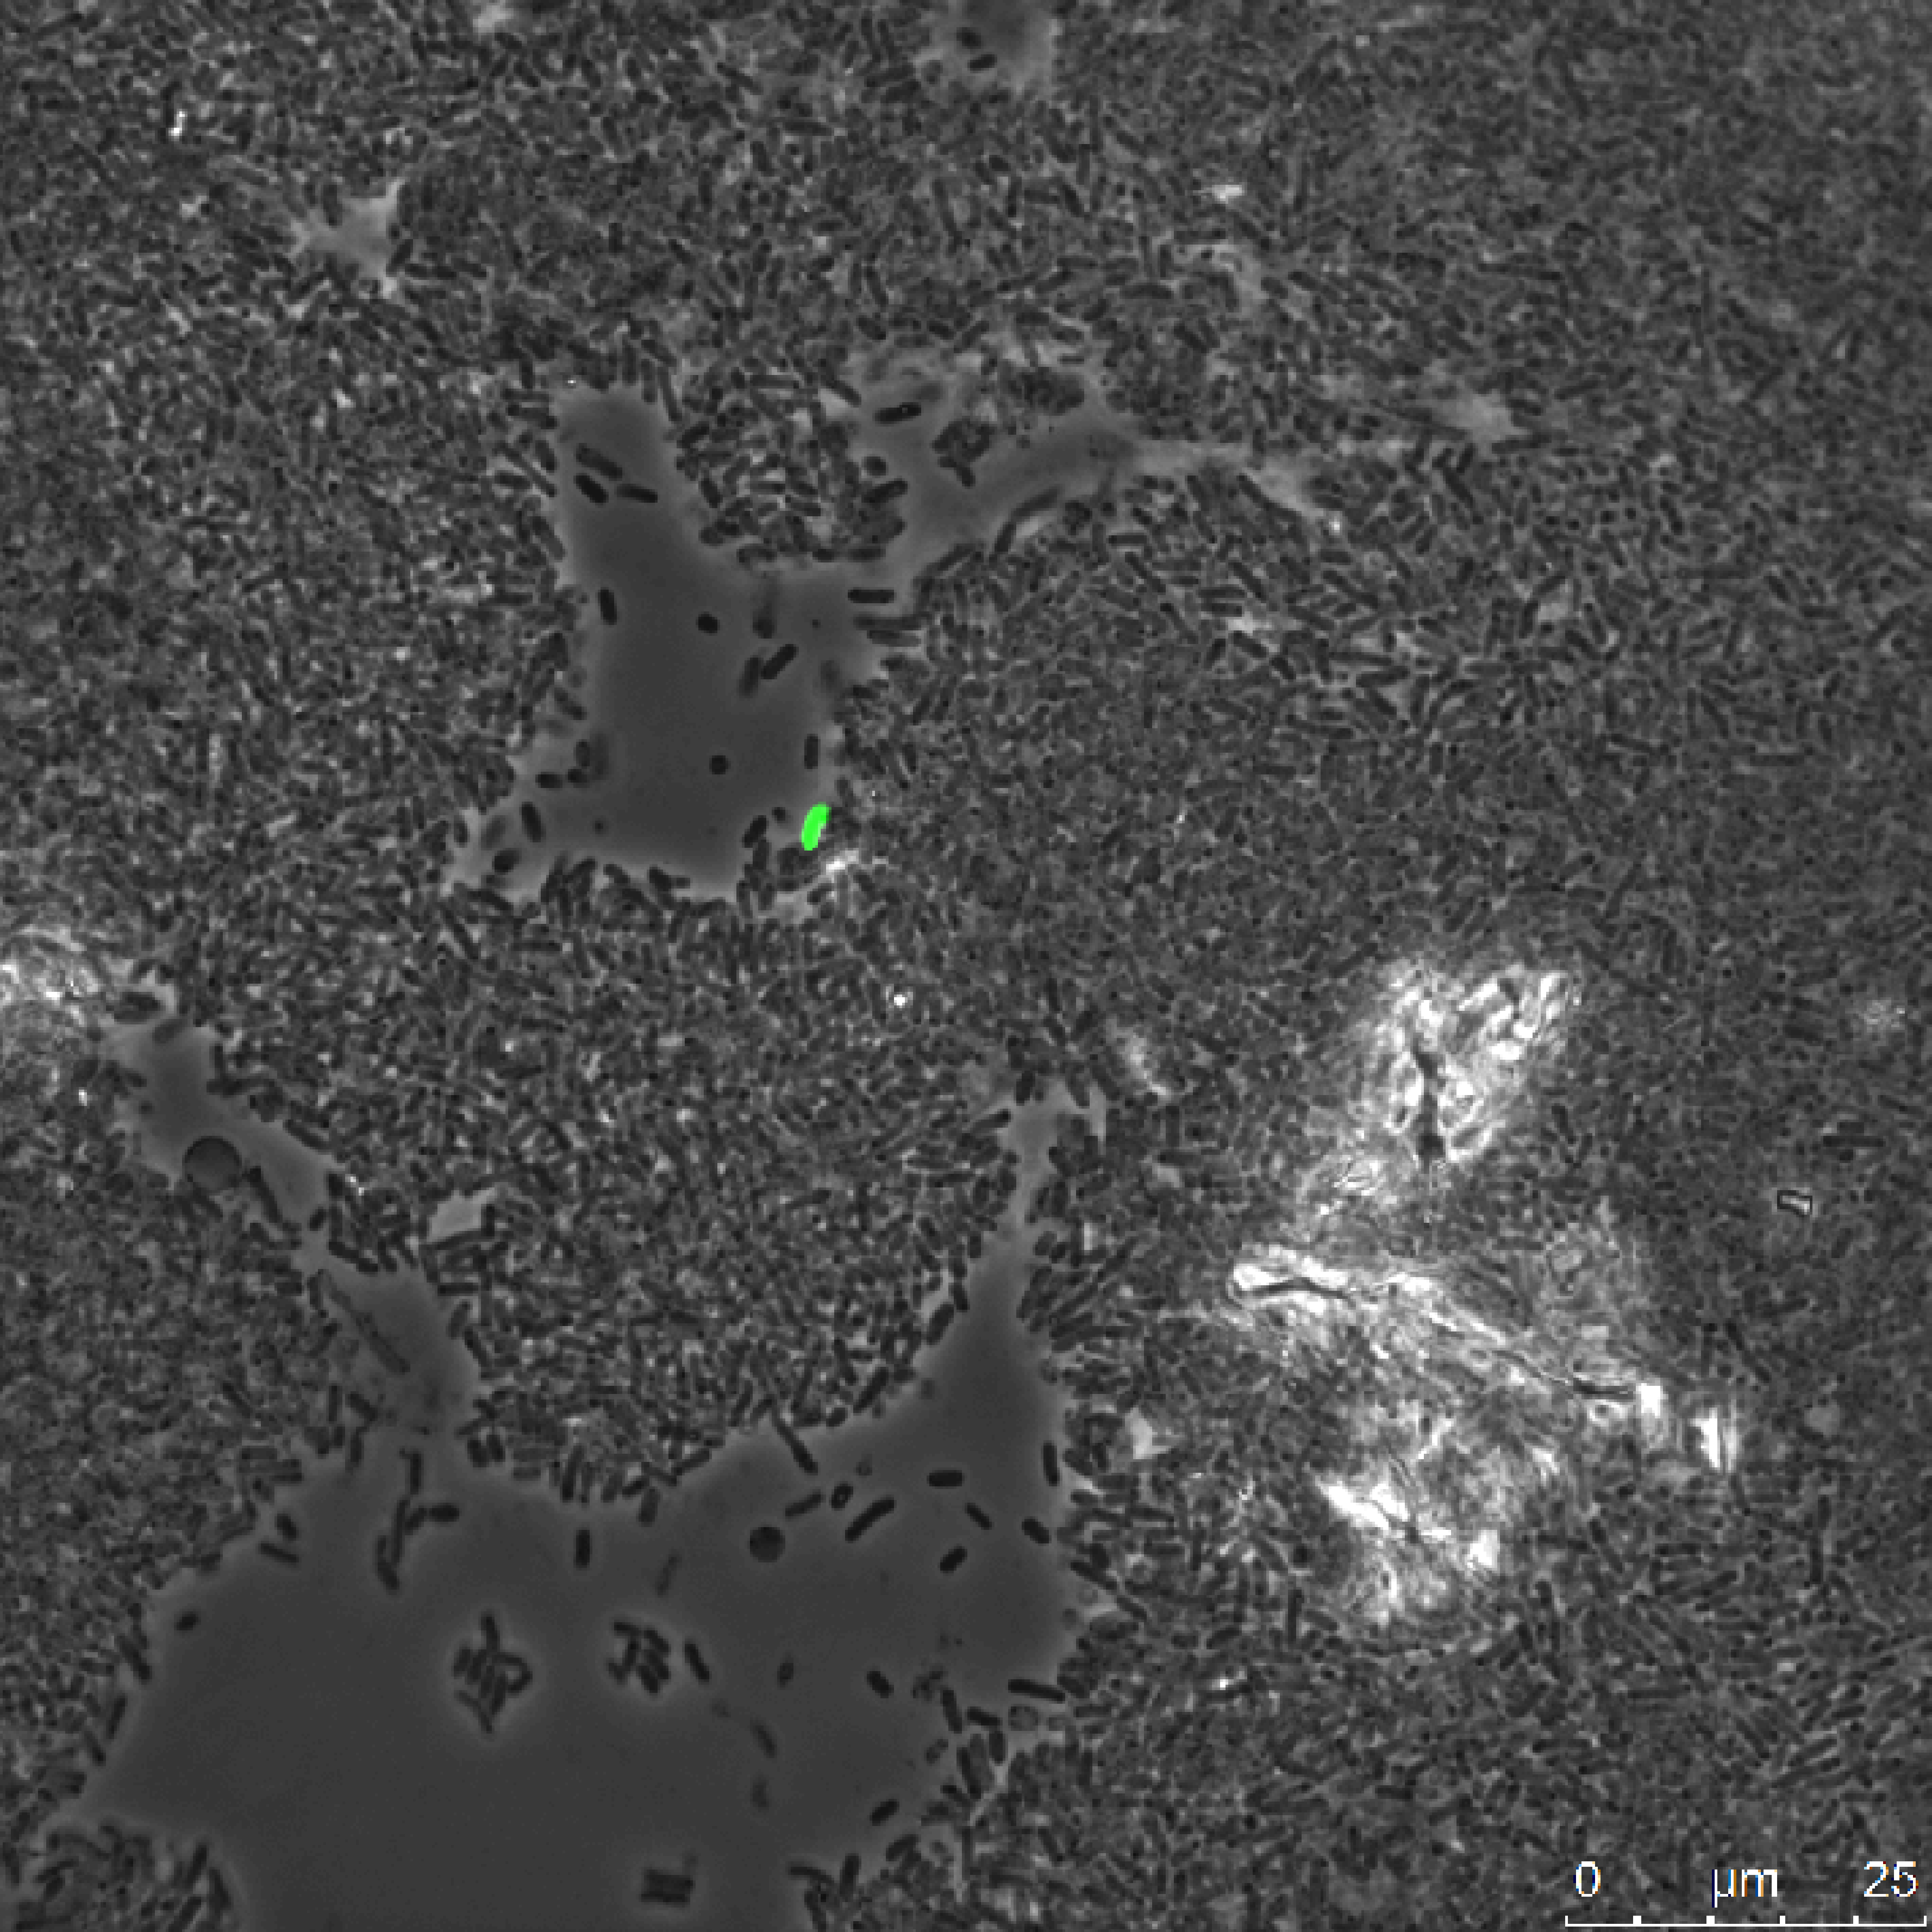
\includegraphics{THAIU1_72HR_2_GREEN.pdf} \\[-0.5ex]

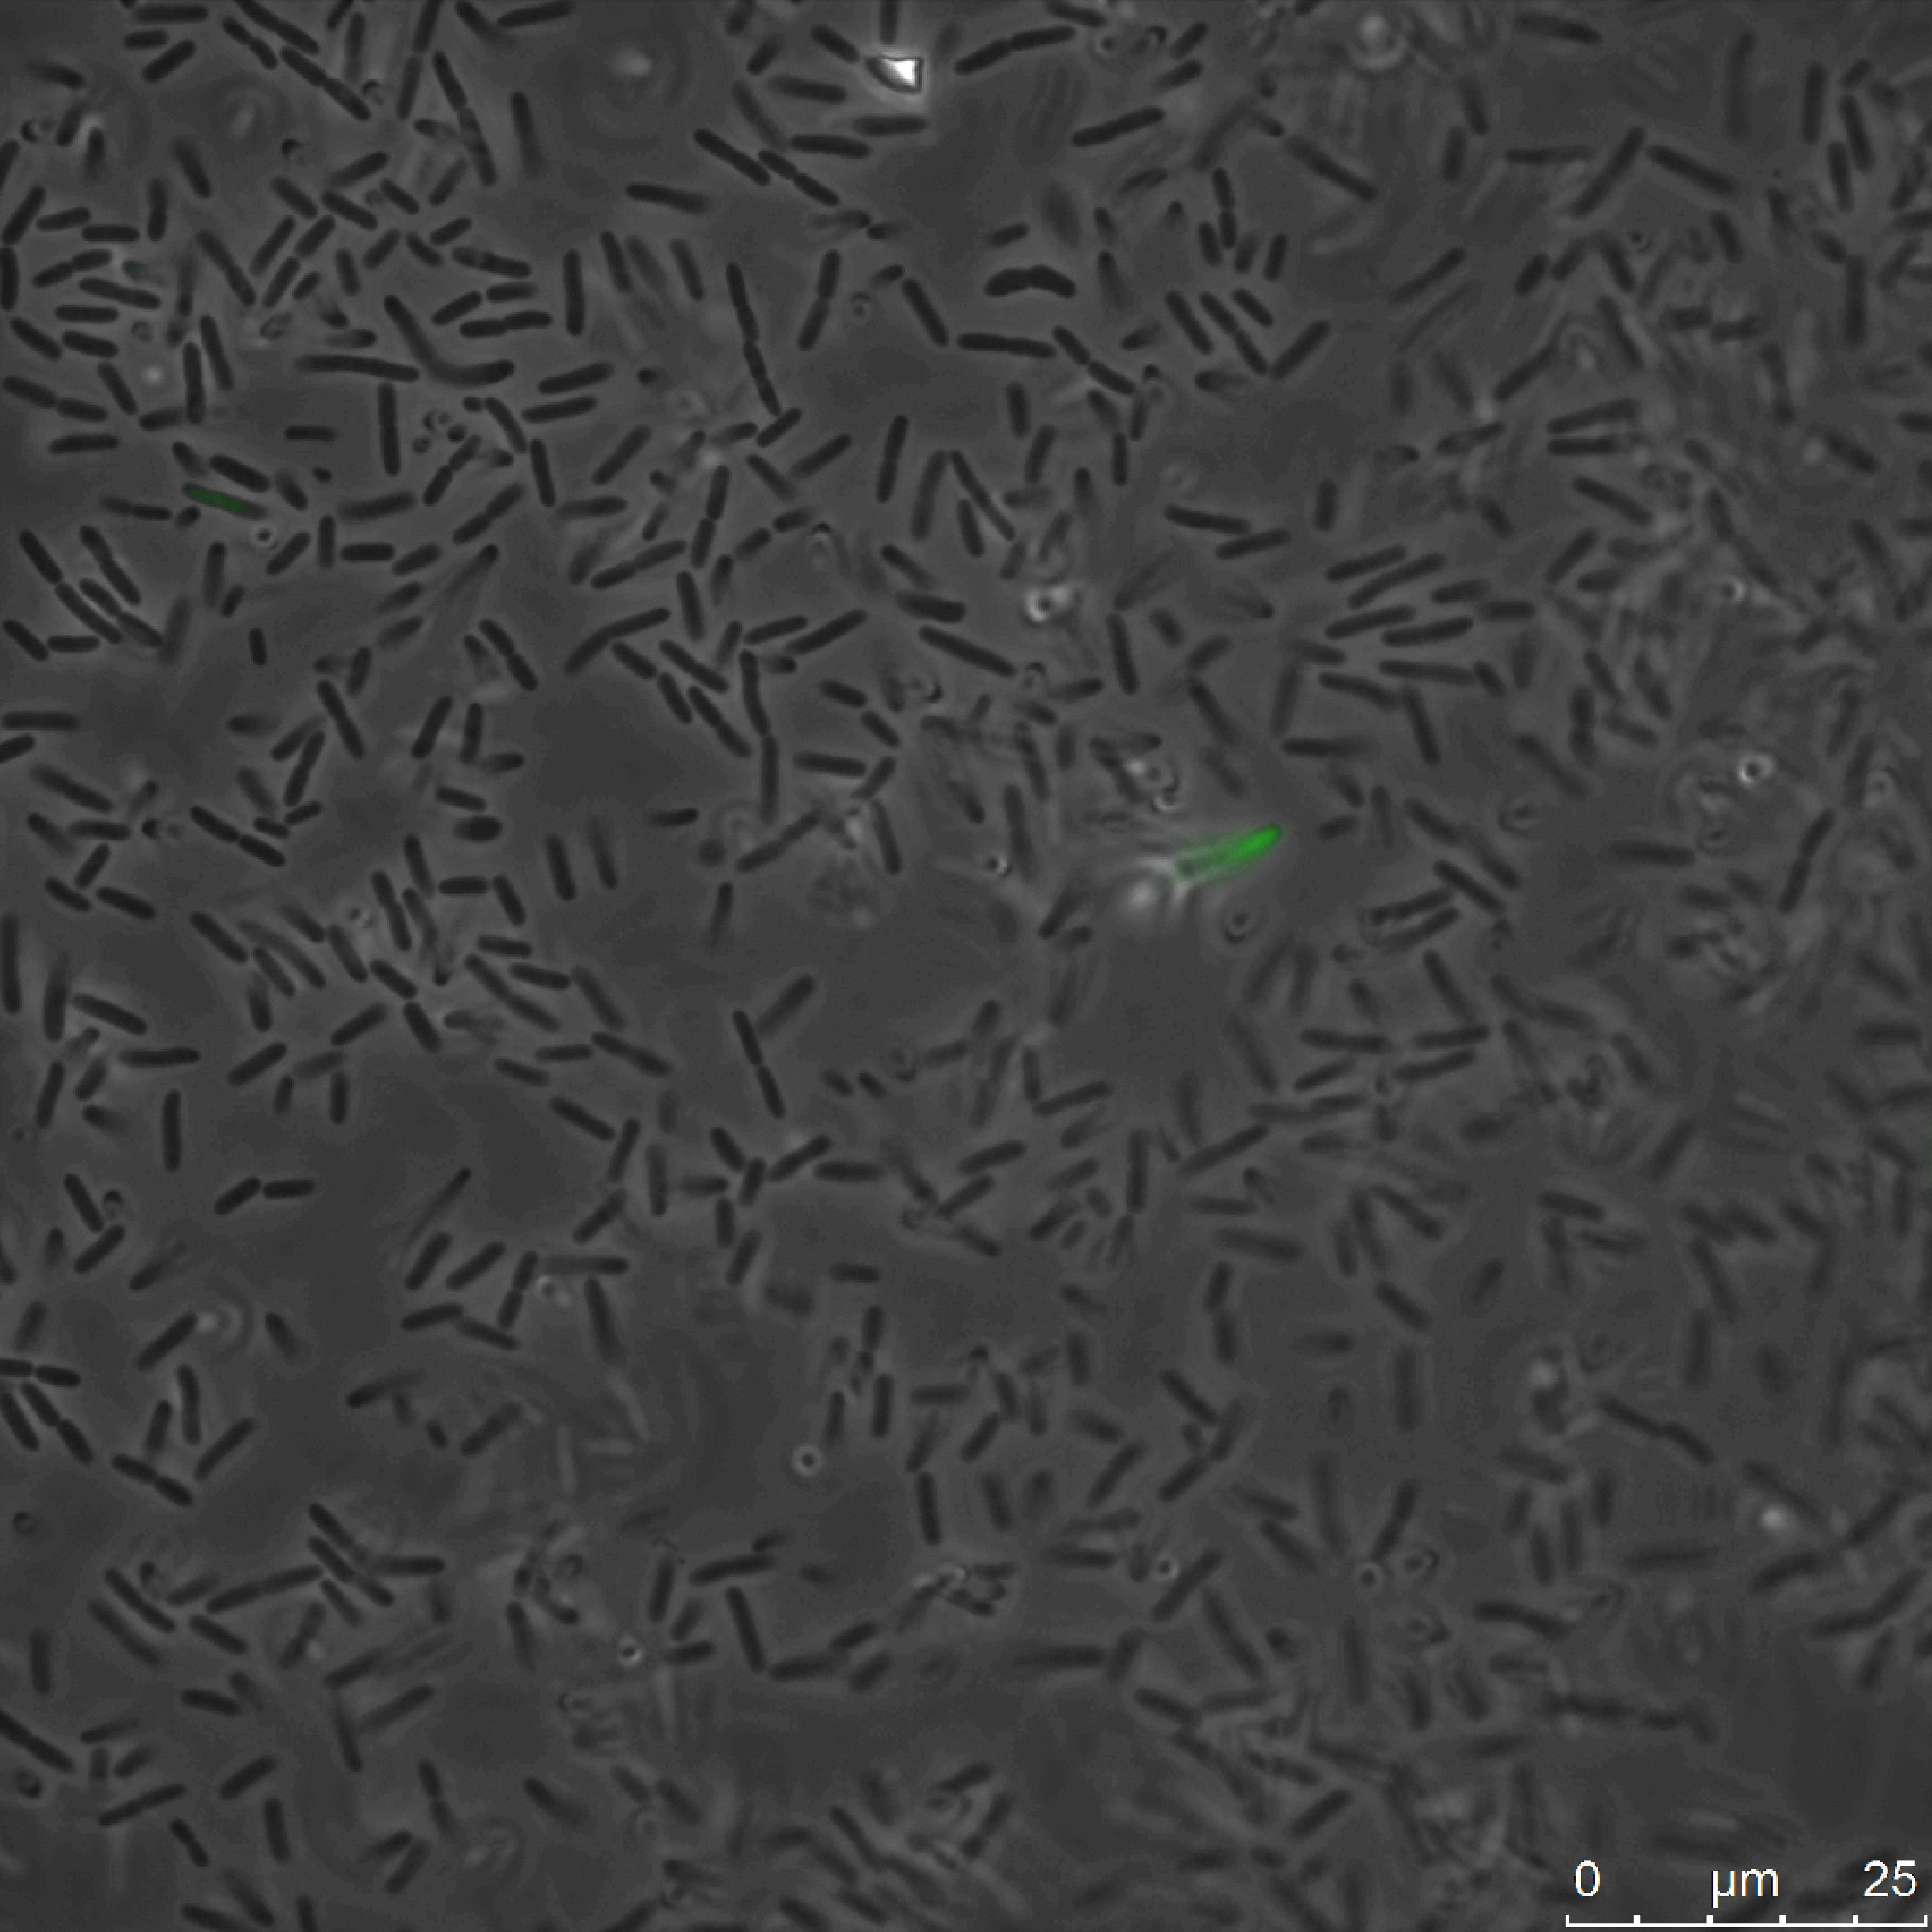
\includegraphics{THAIU1_3_GREEN.pdf} &%
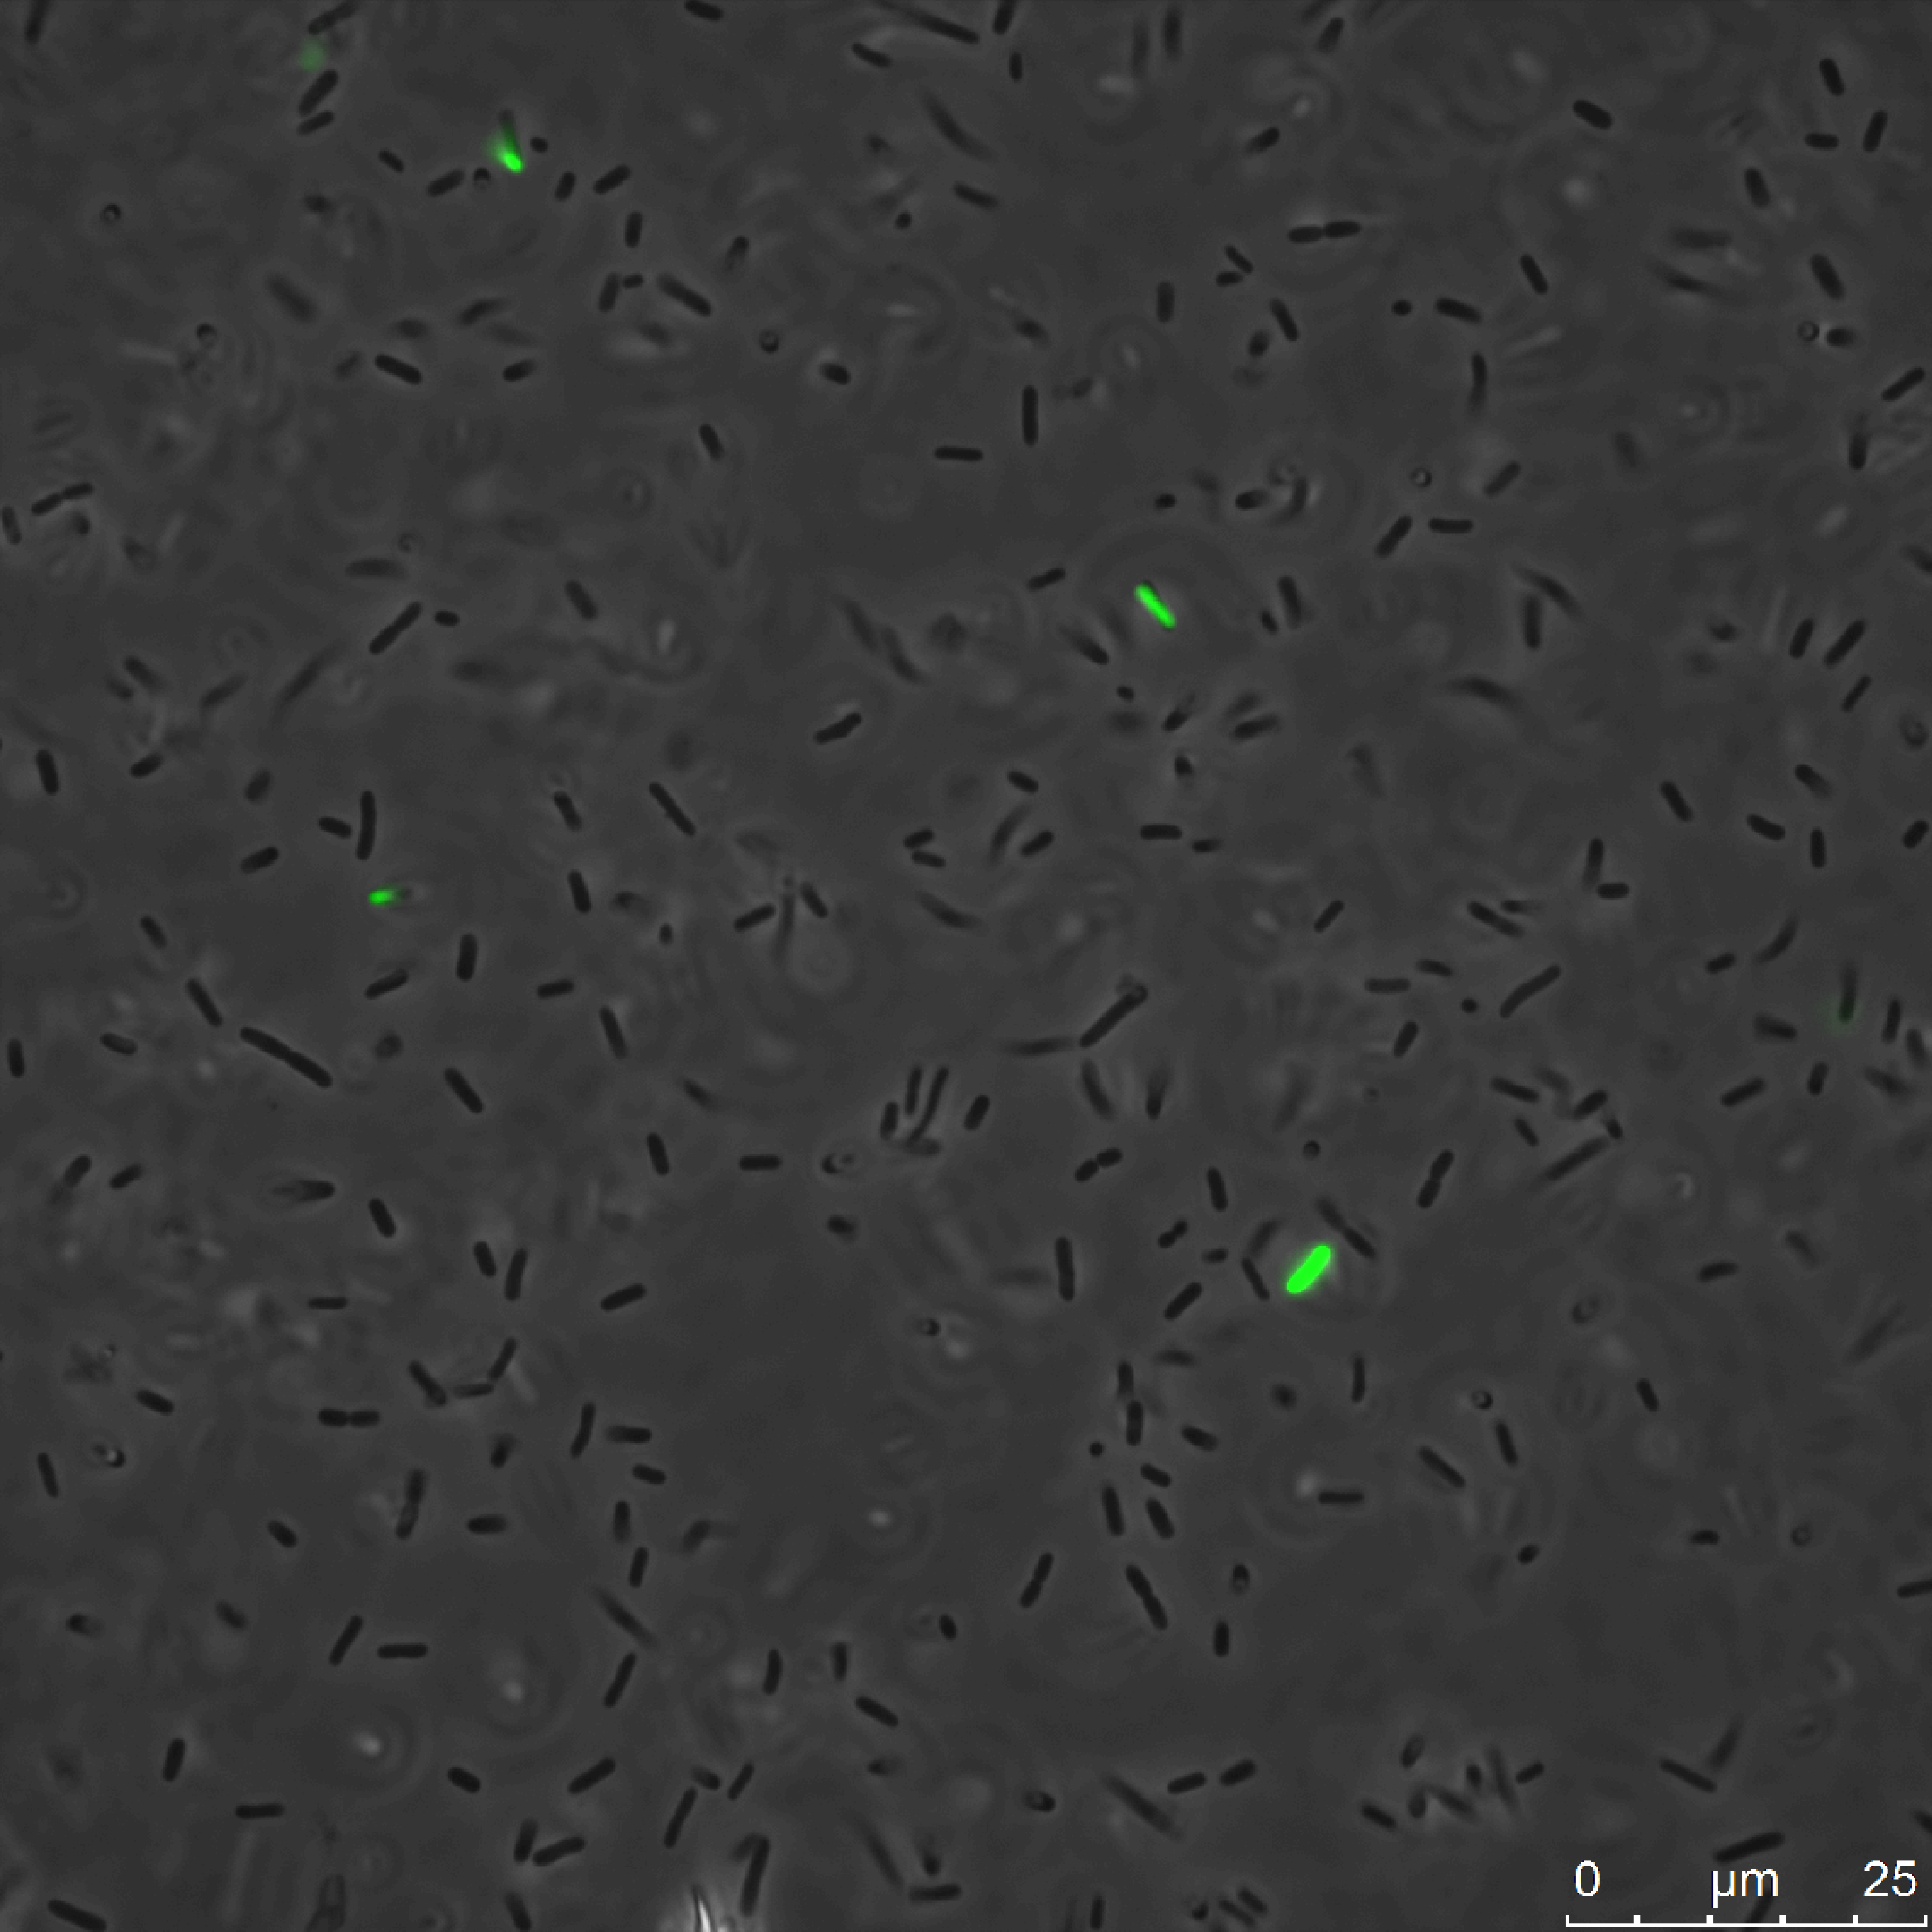
\includegraphics{THAIU1_5HR_3_GREEN.pdf} &%
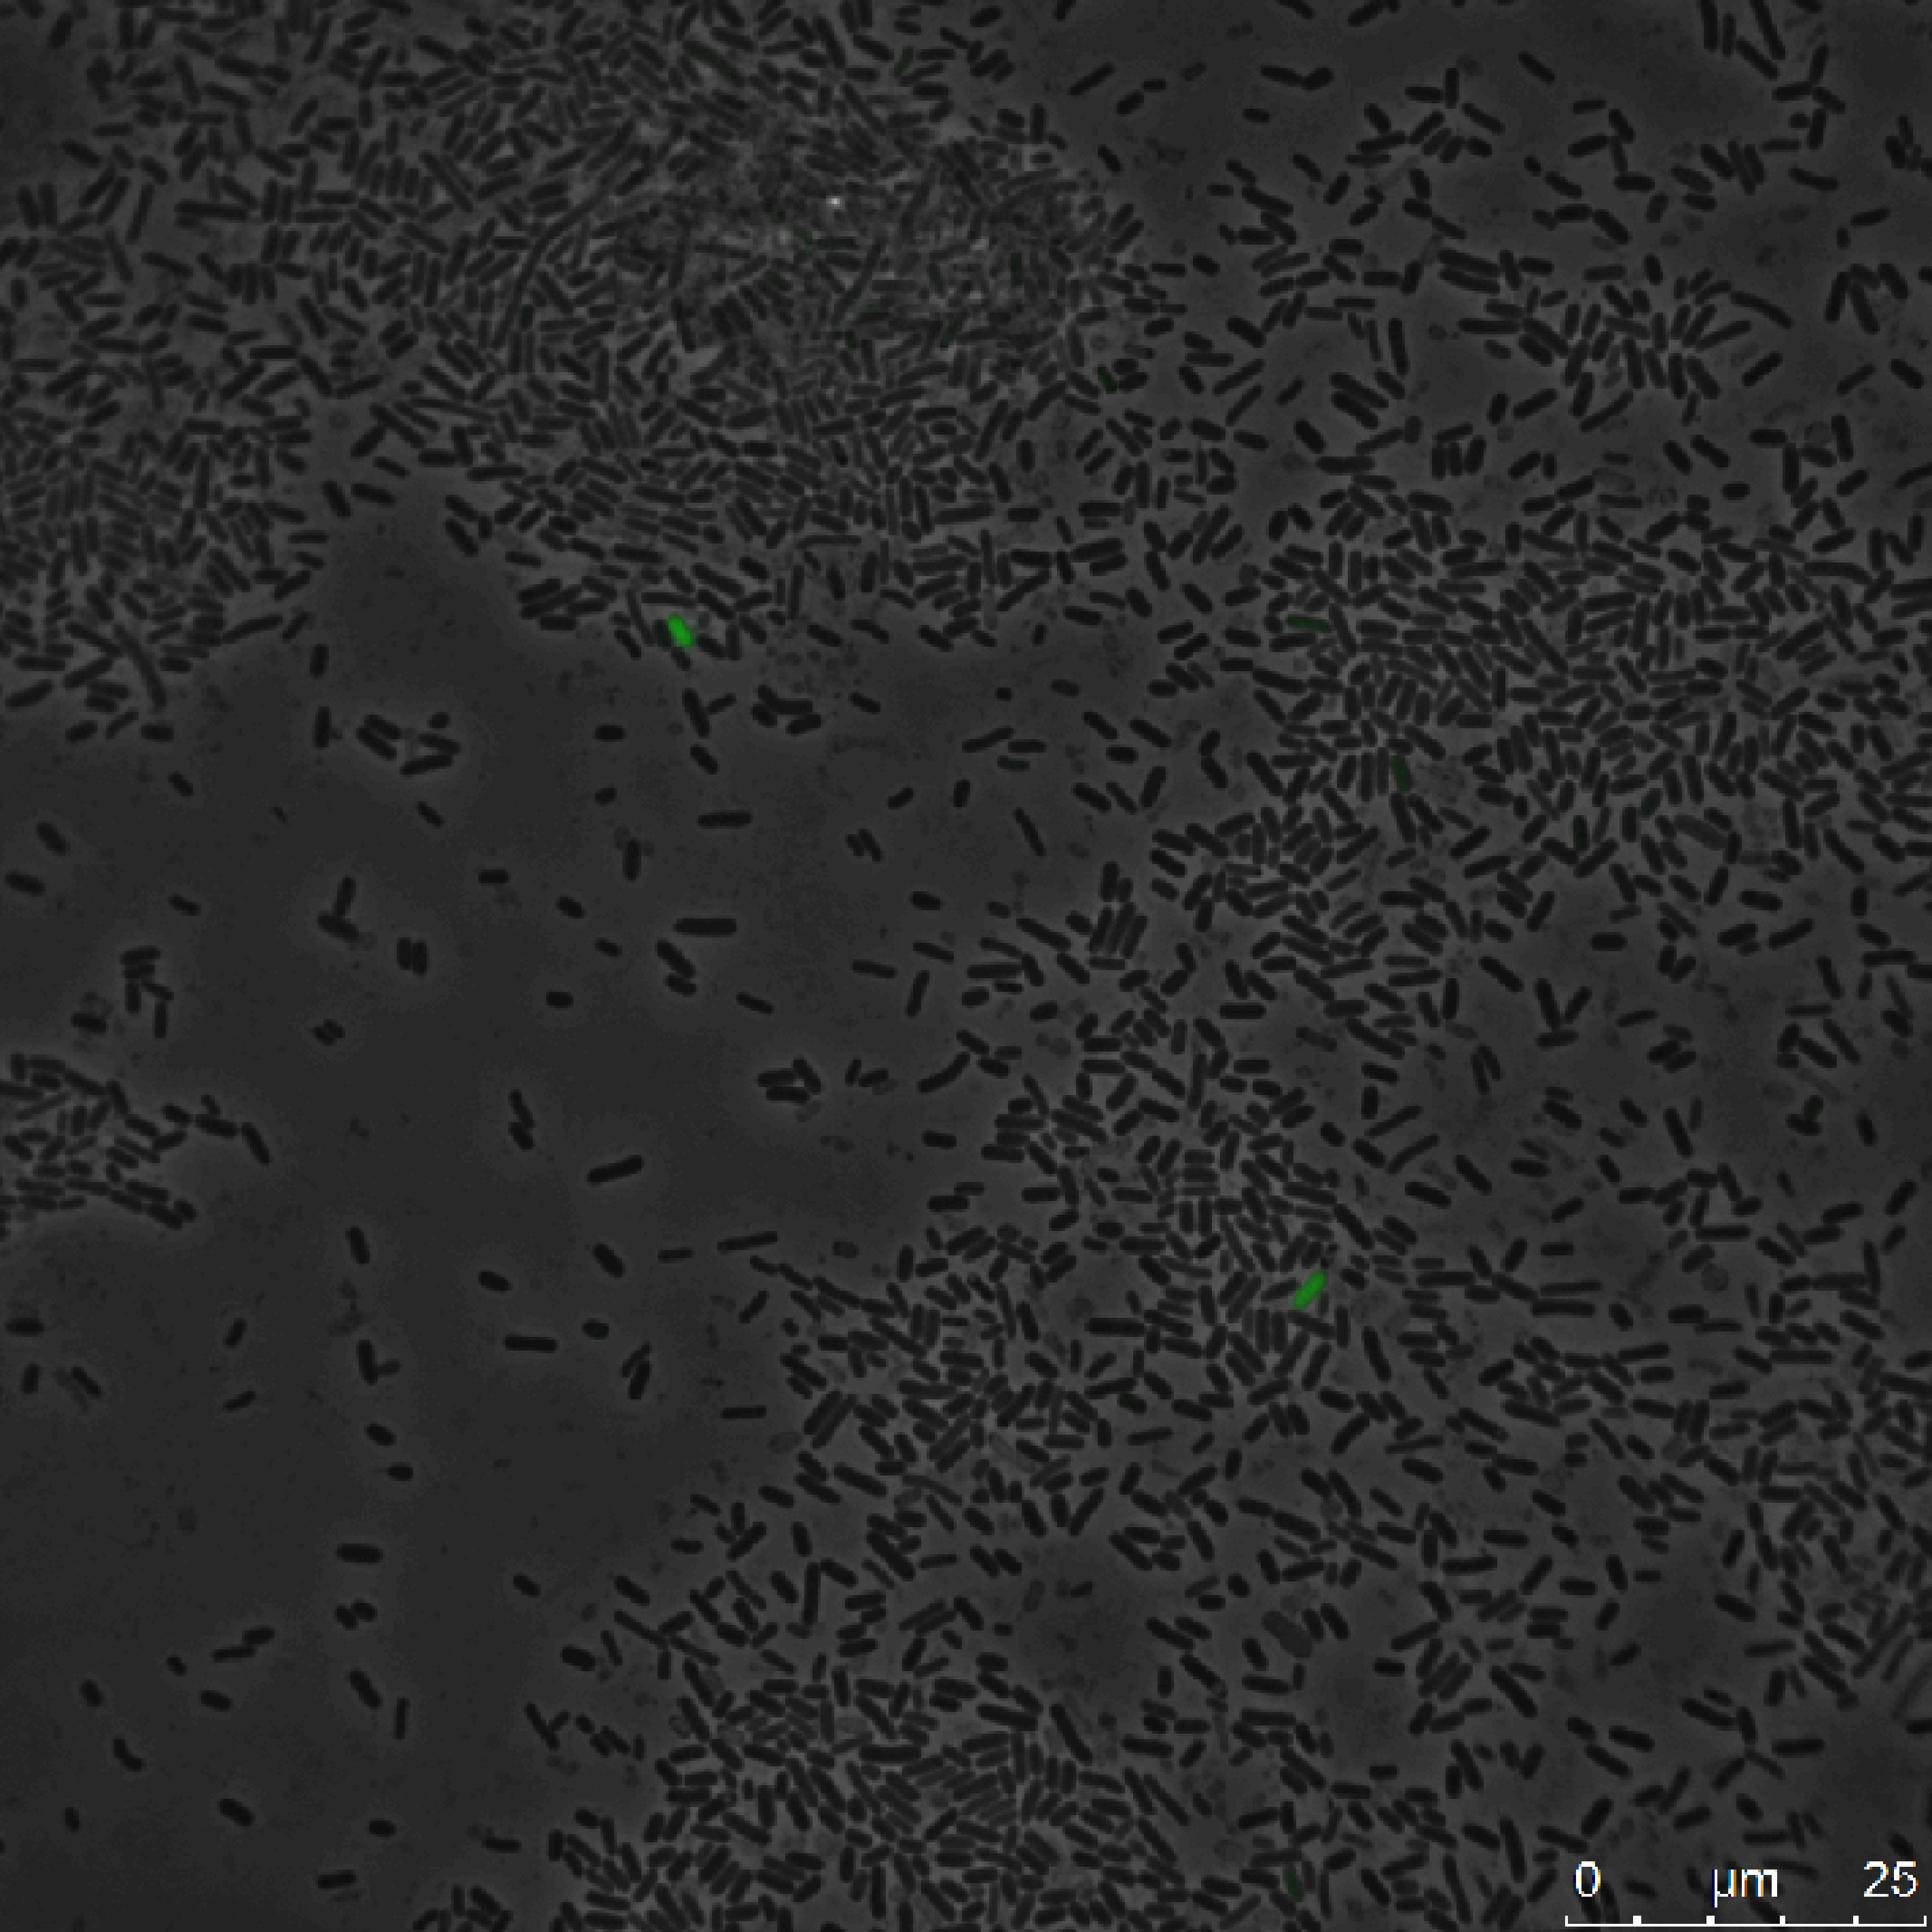
\includegraphics{THAIU1_24HR_6_GREEN.pdf} &%
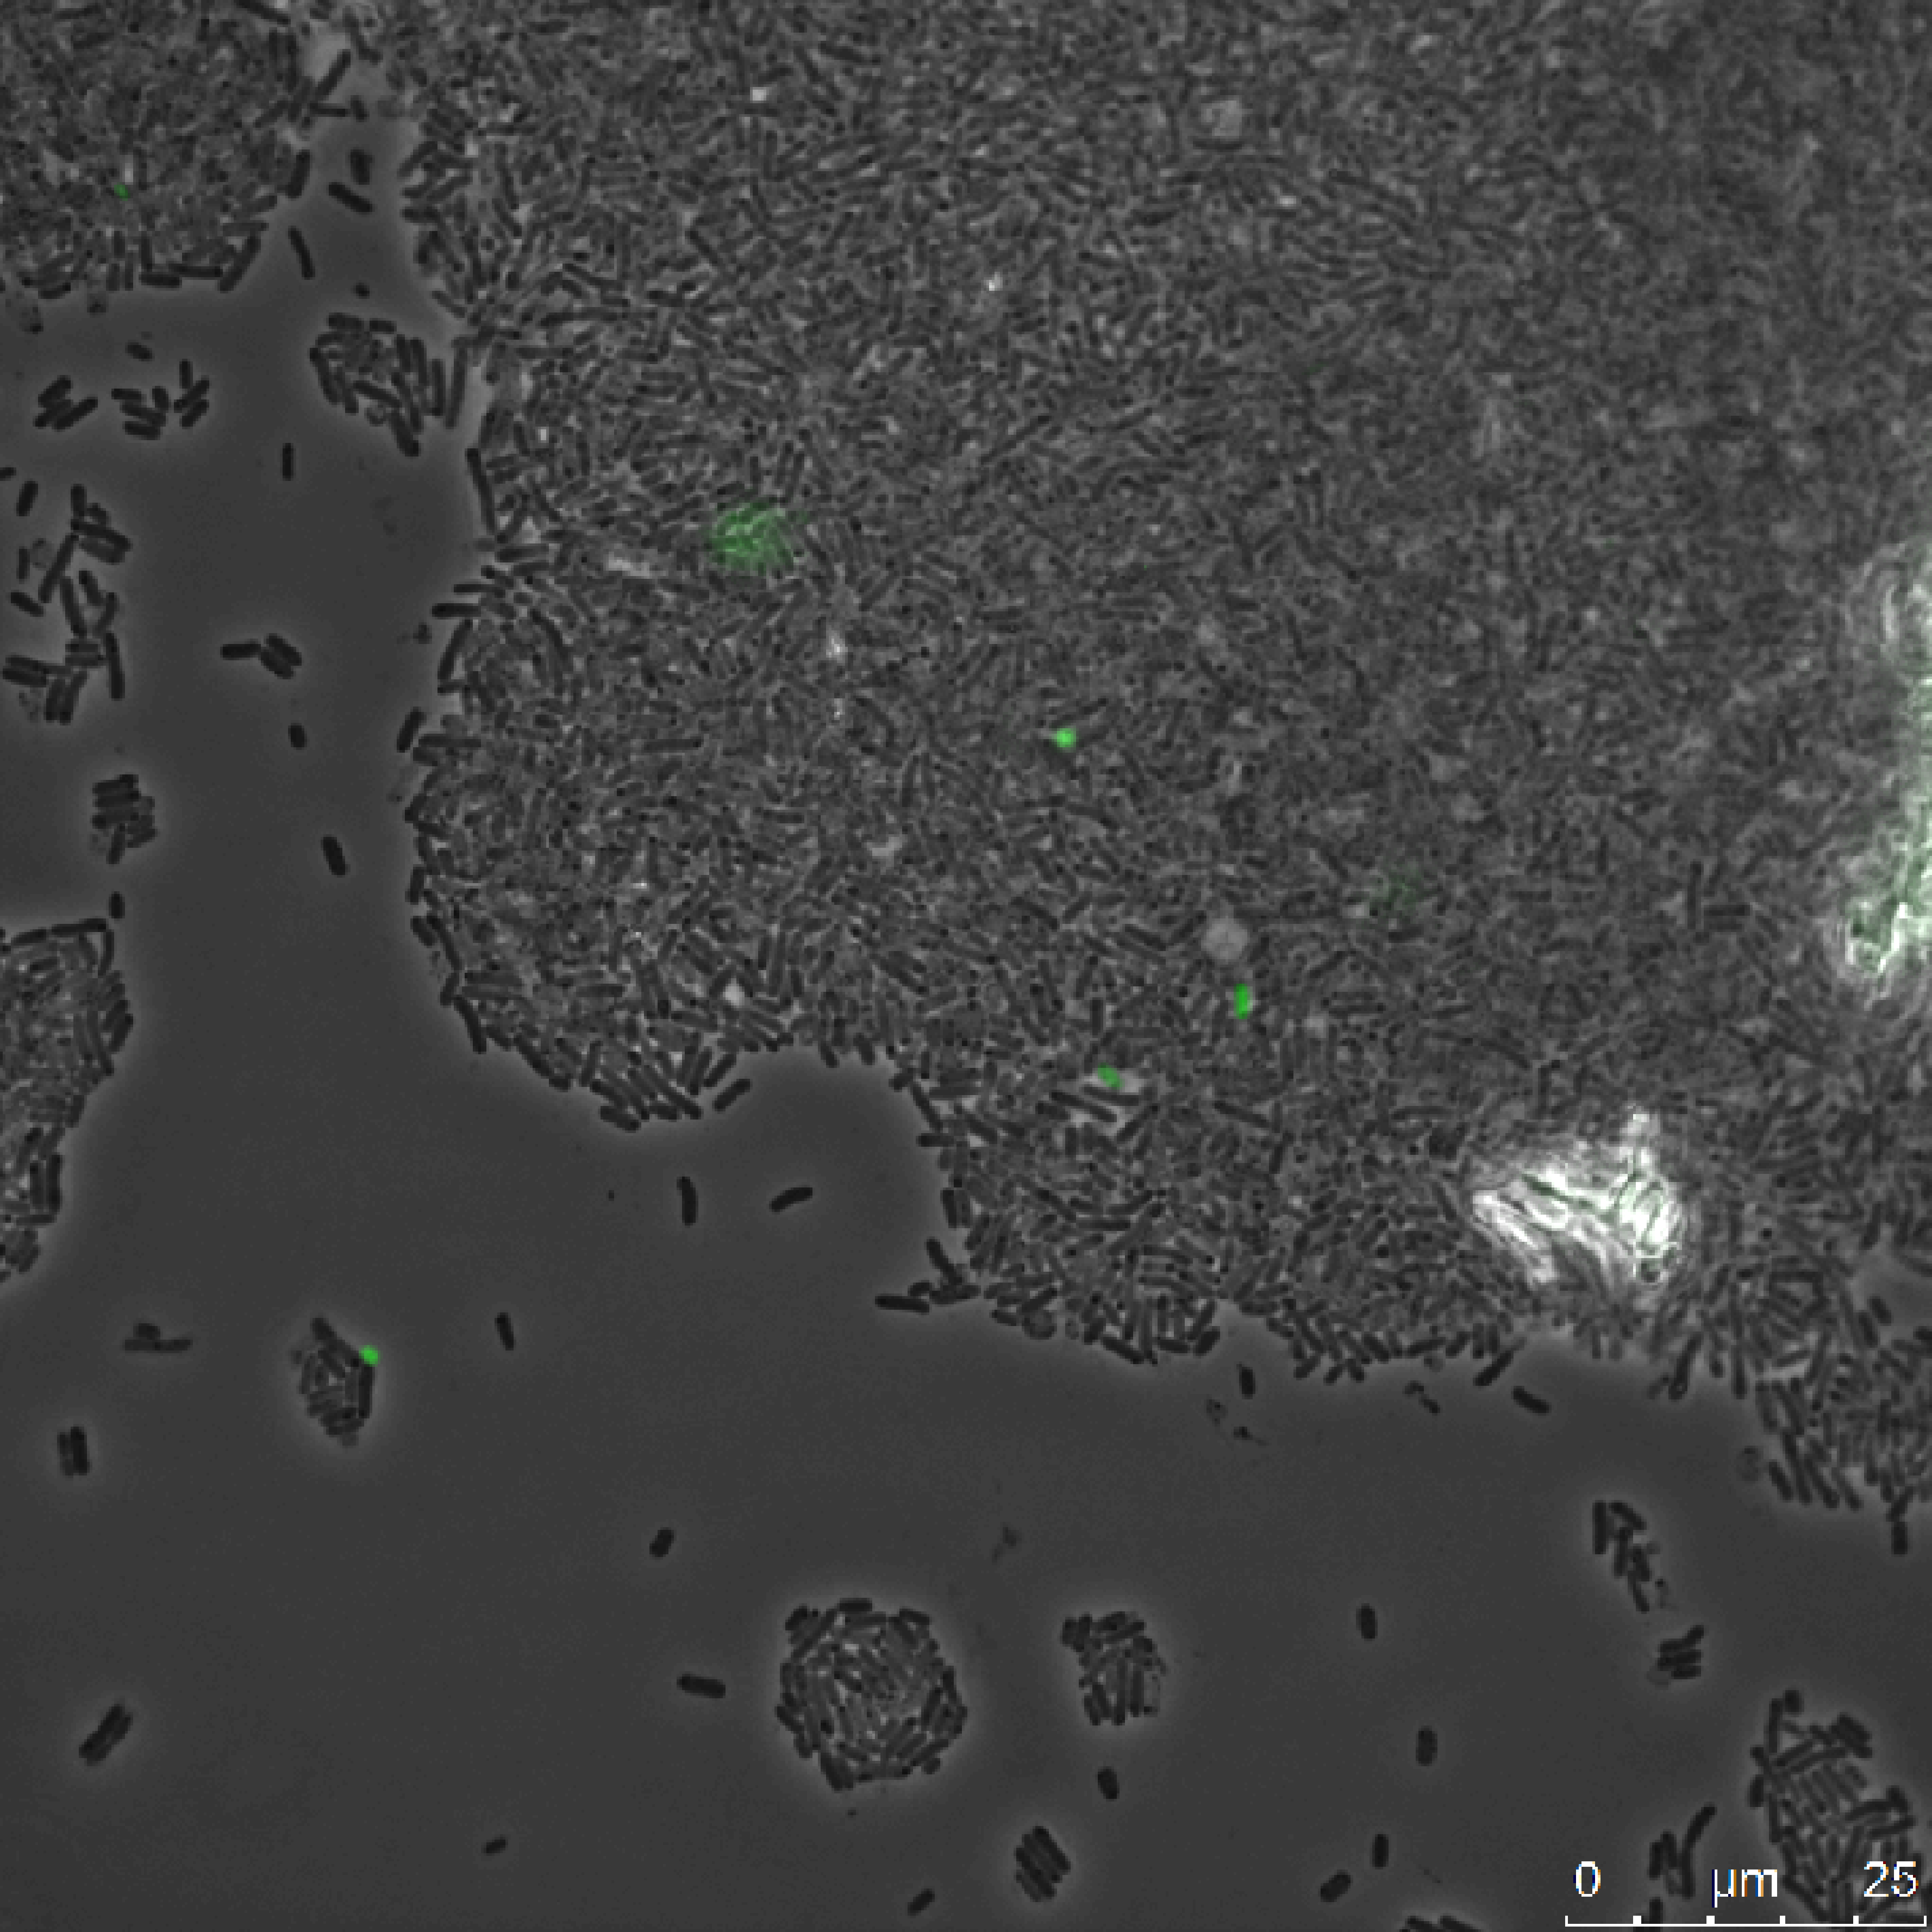
\includegraphics{THAIU1_72HR_3_GREEN.pdf} \\[-0.5ex]

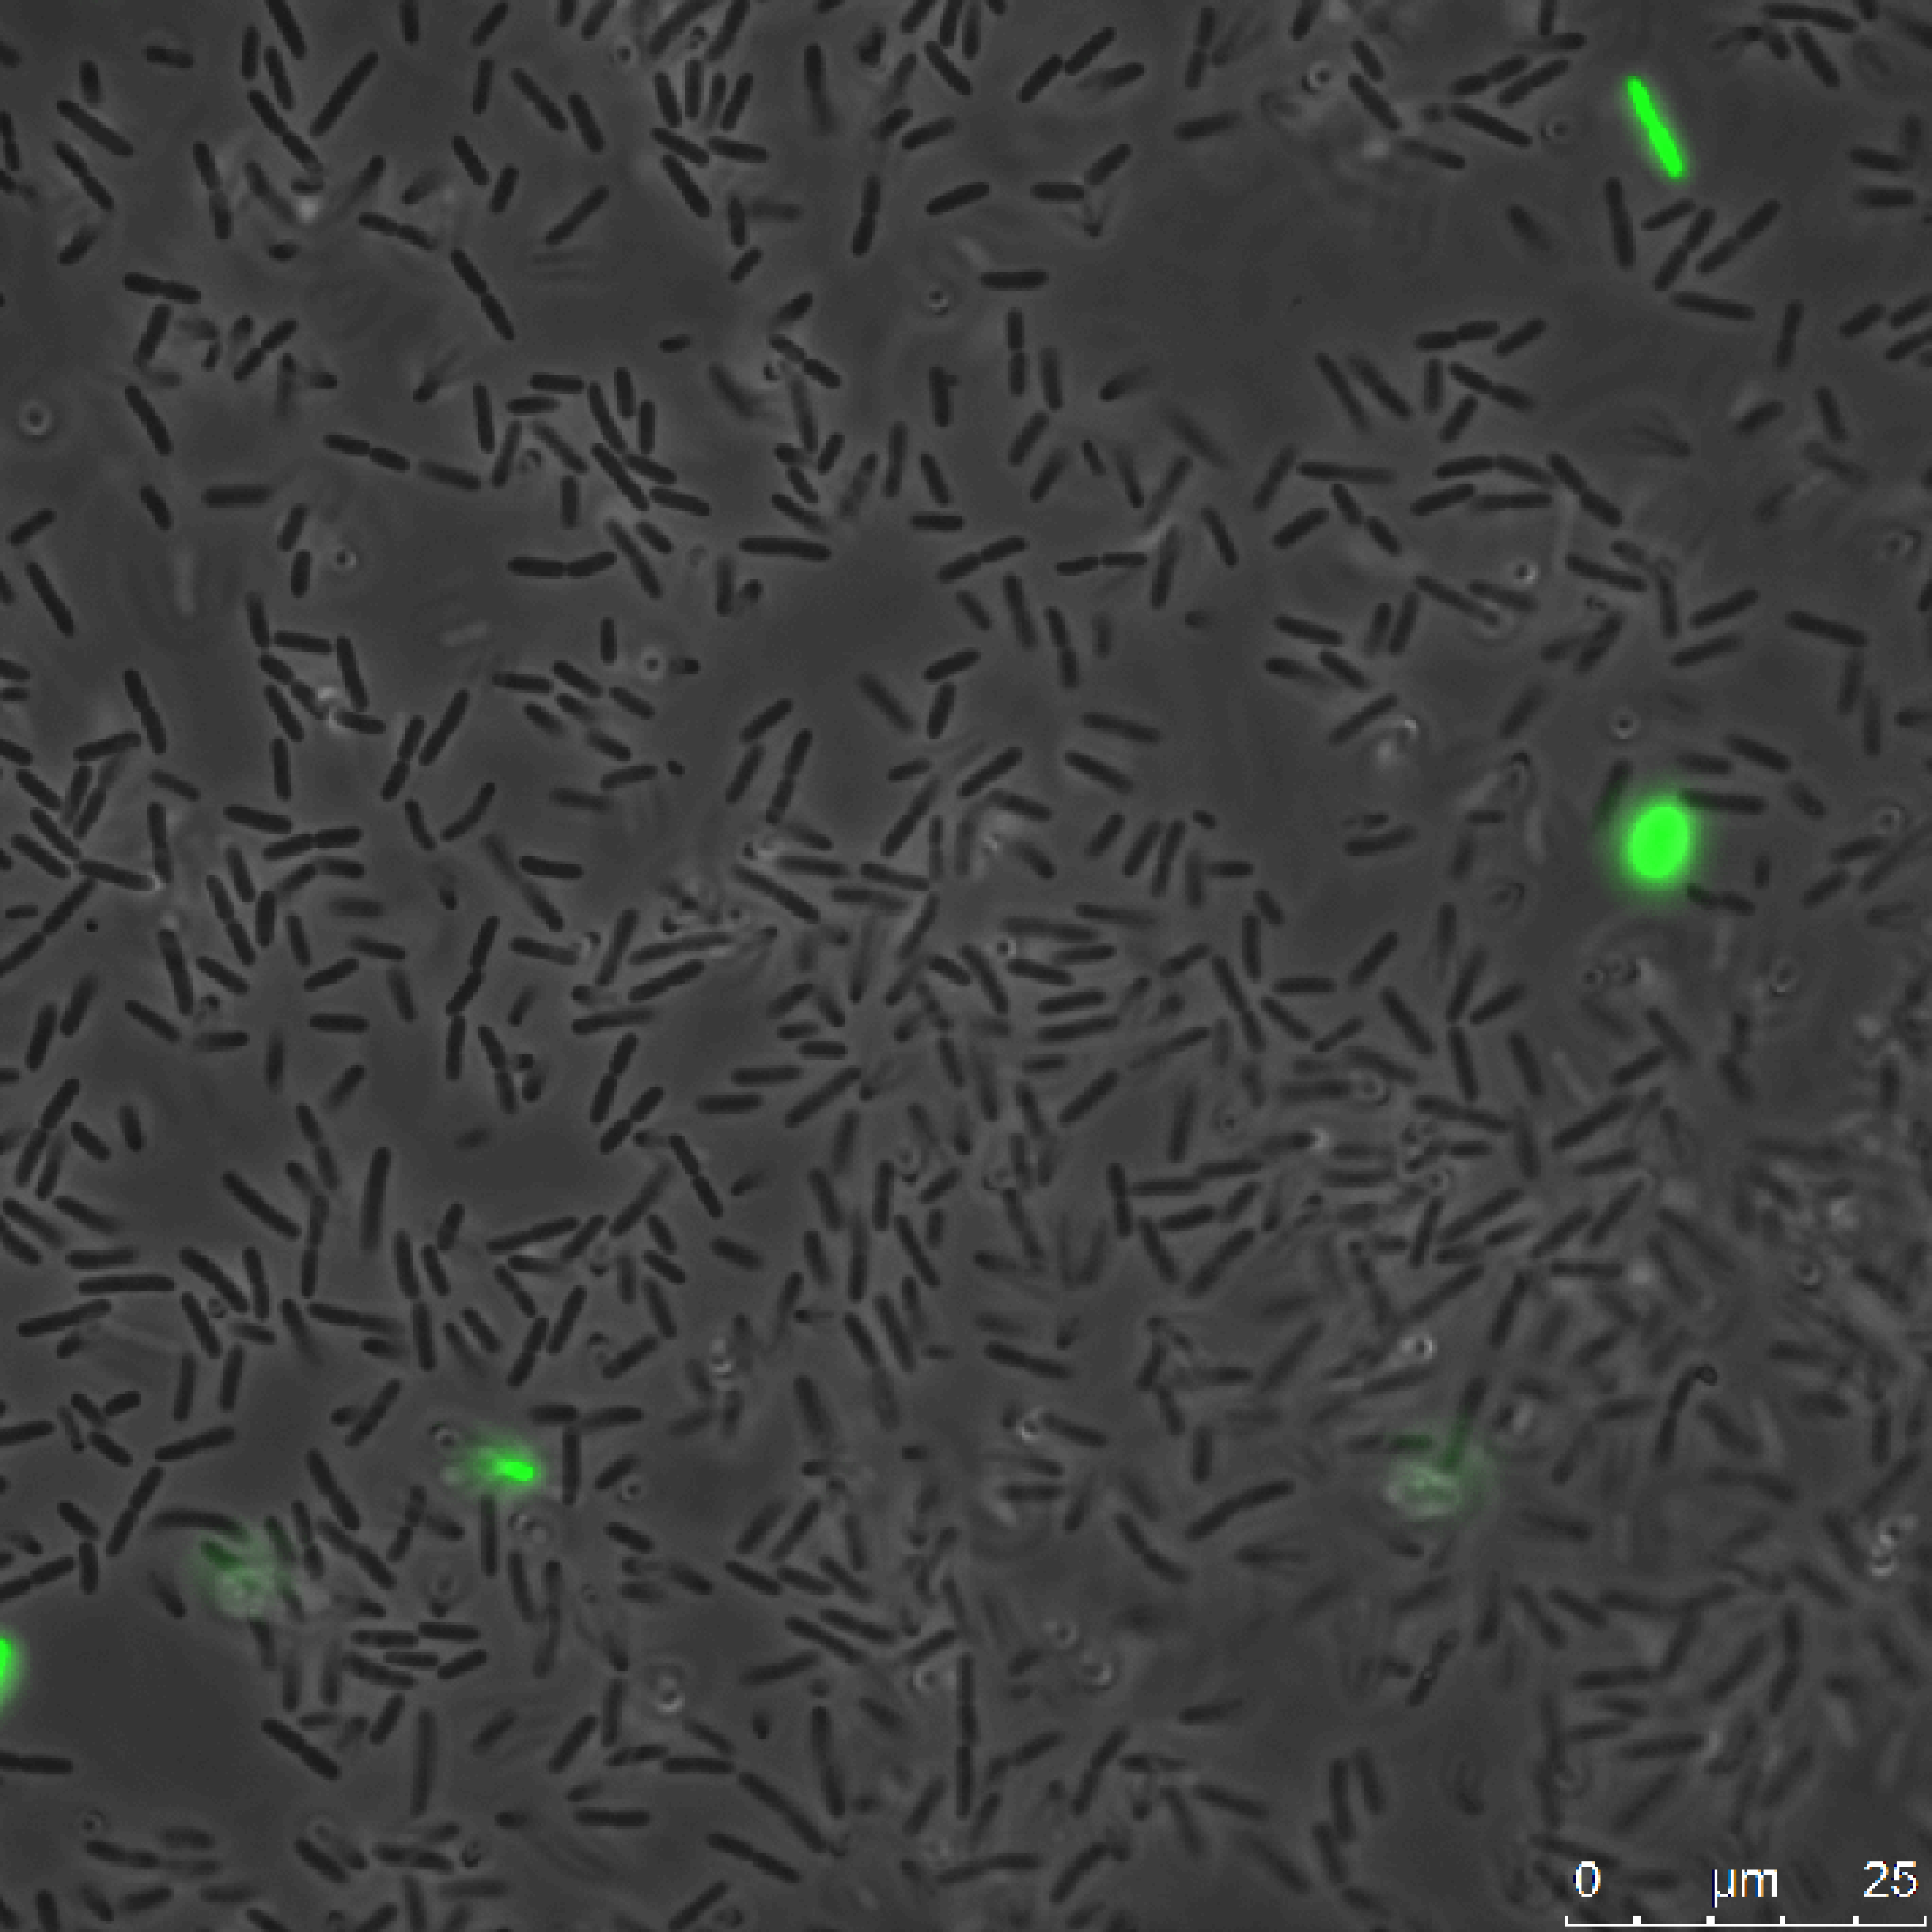
\includegraphics{THAIU1_4_GREEN.pdf} &%
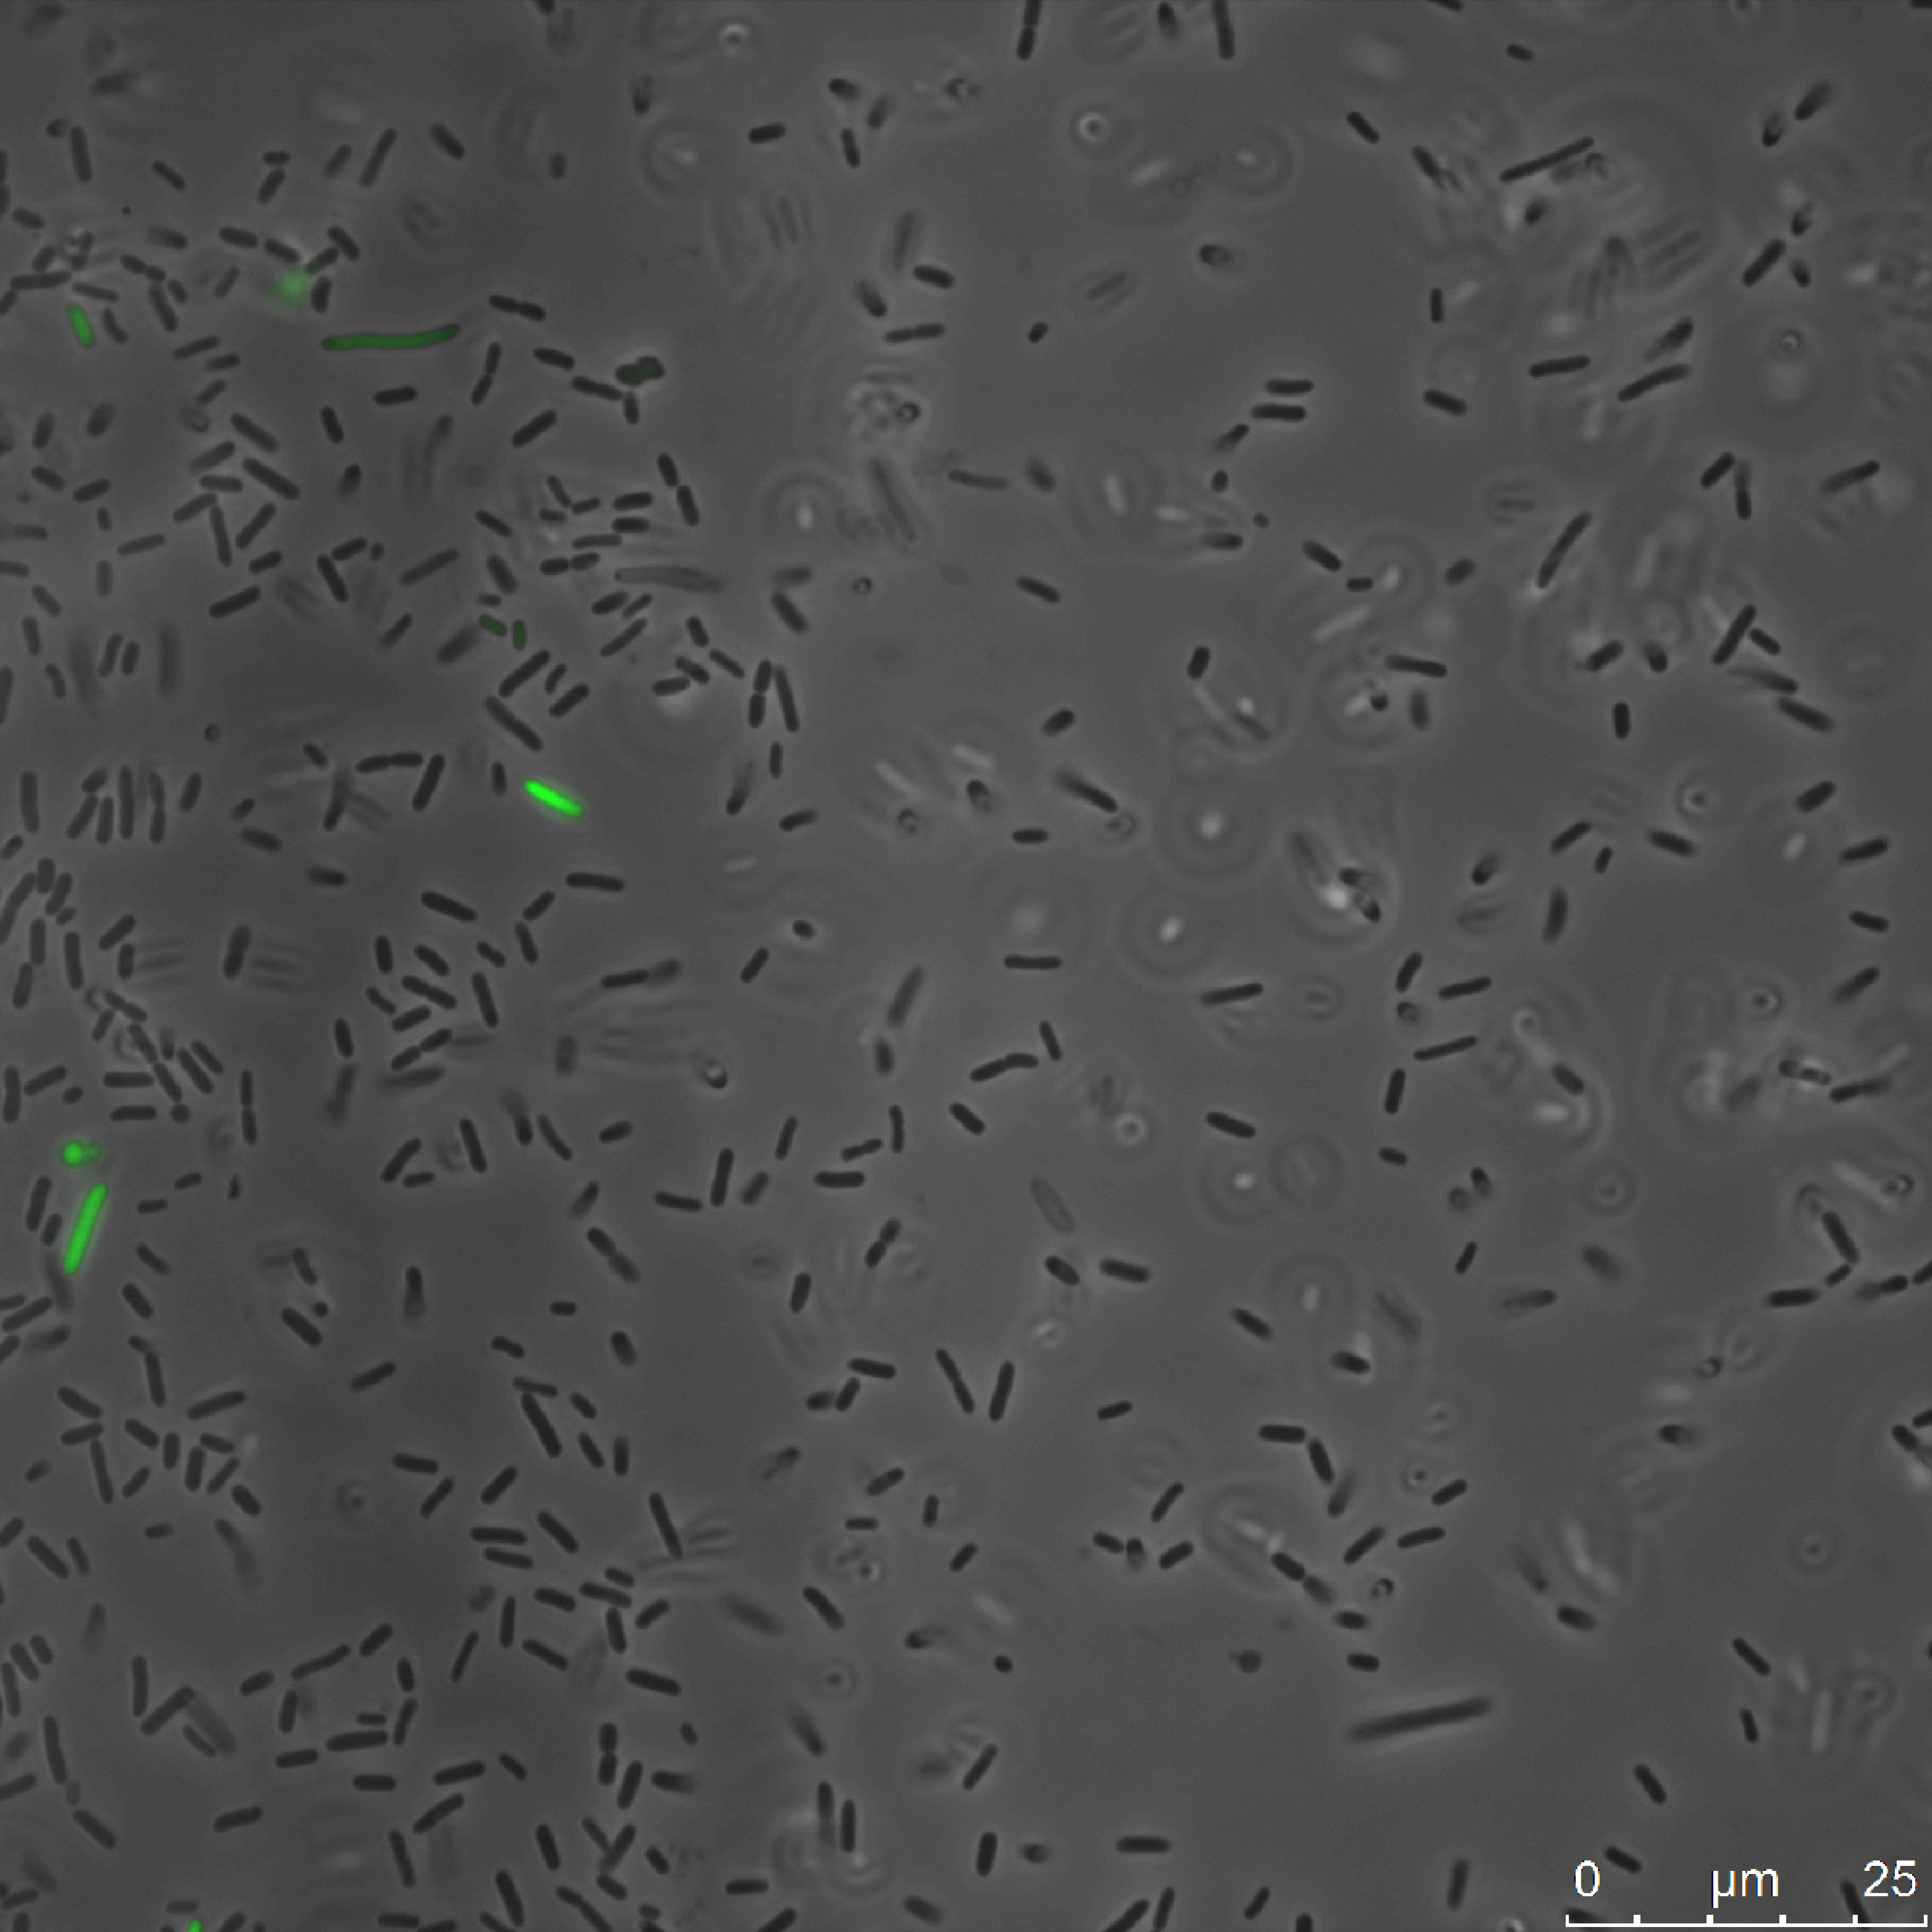
\includegraphics{THAIU1_5HR_6_GREEN.pdf} &%
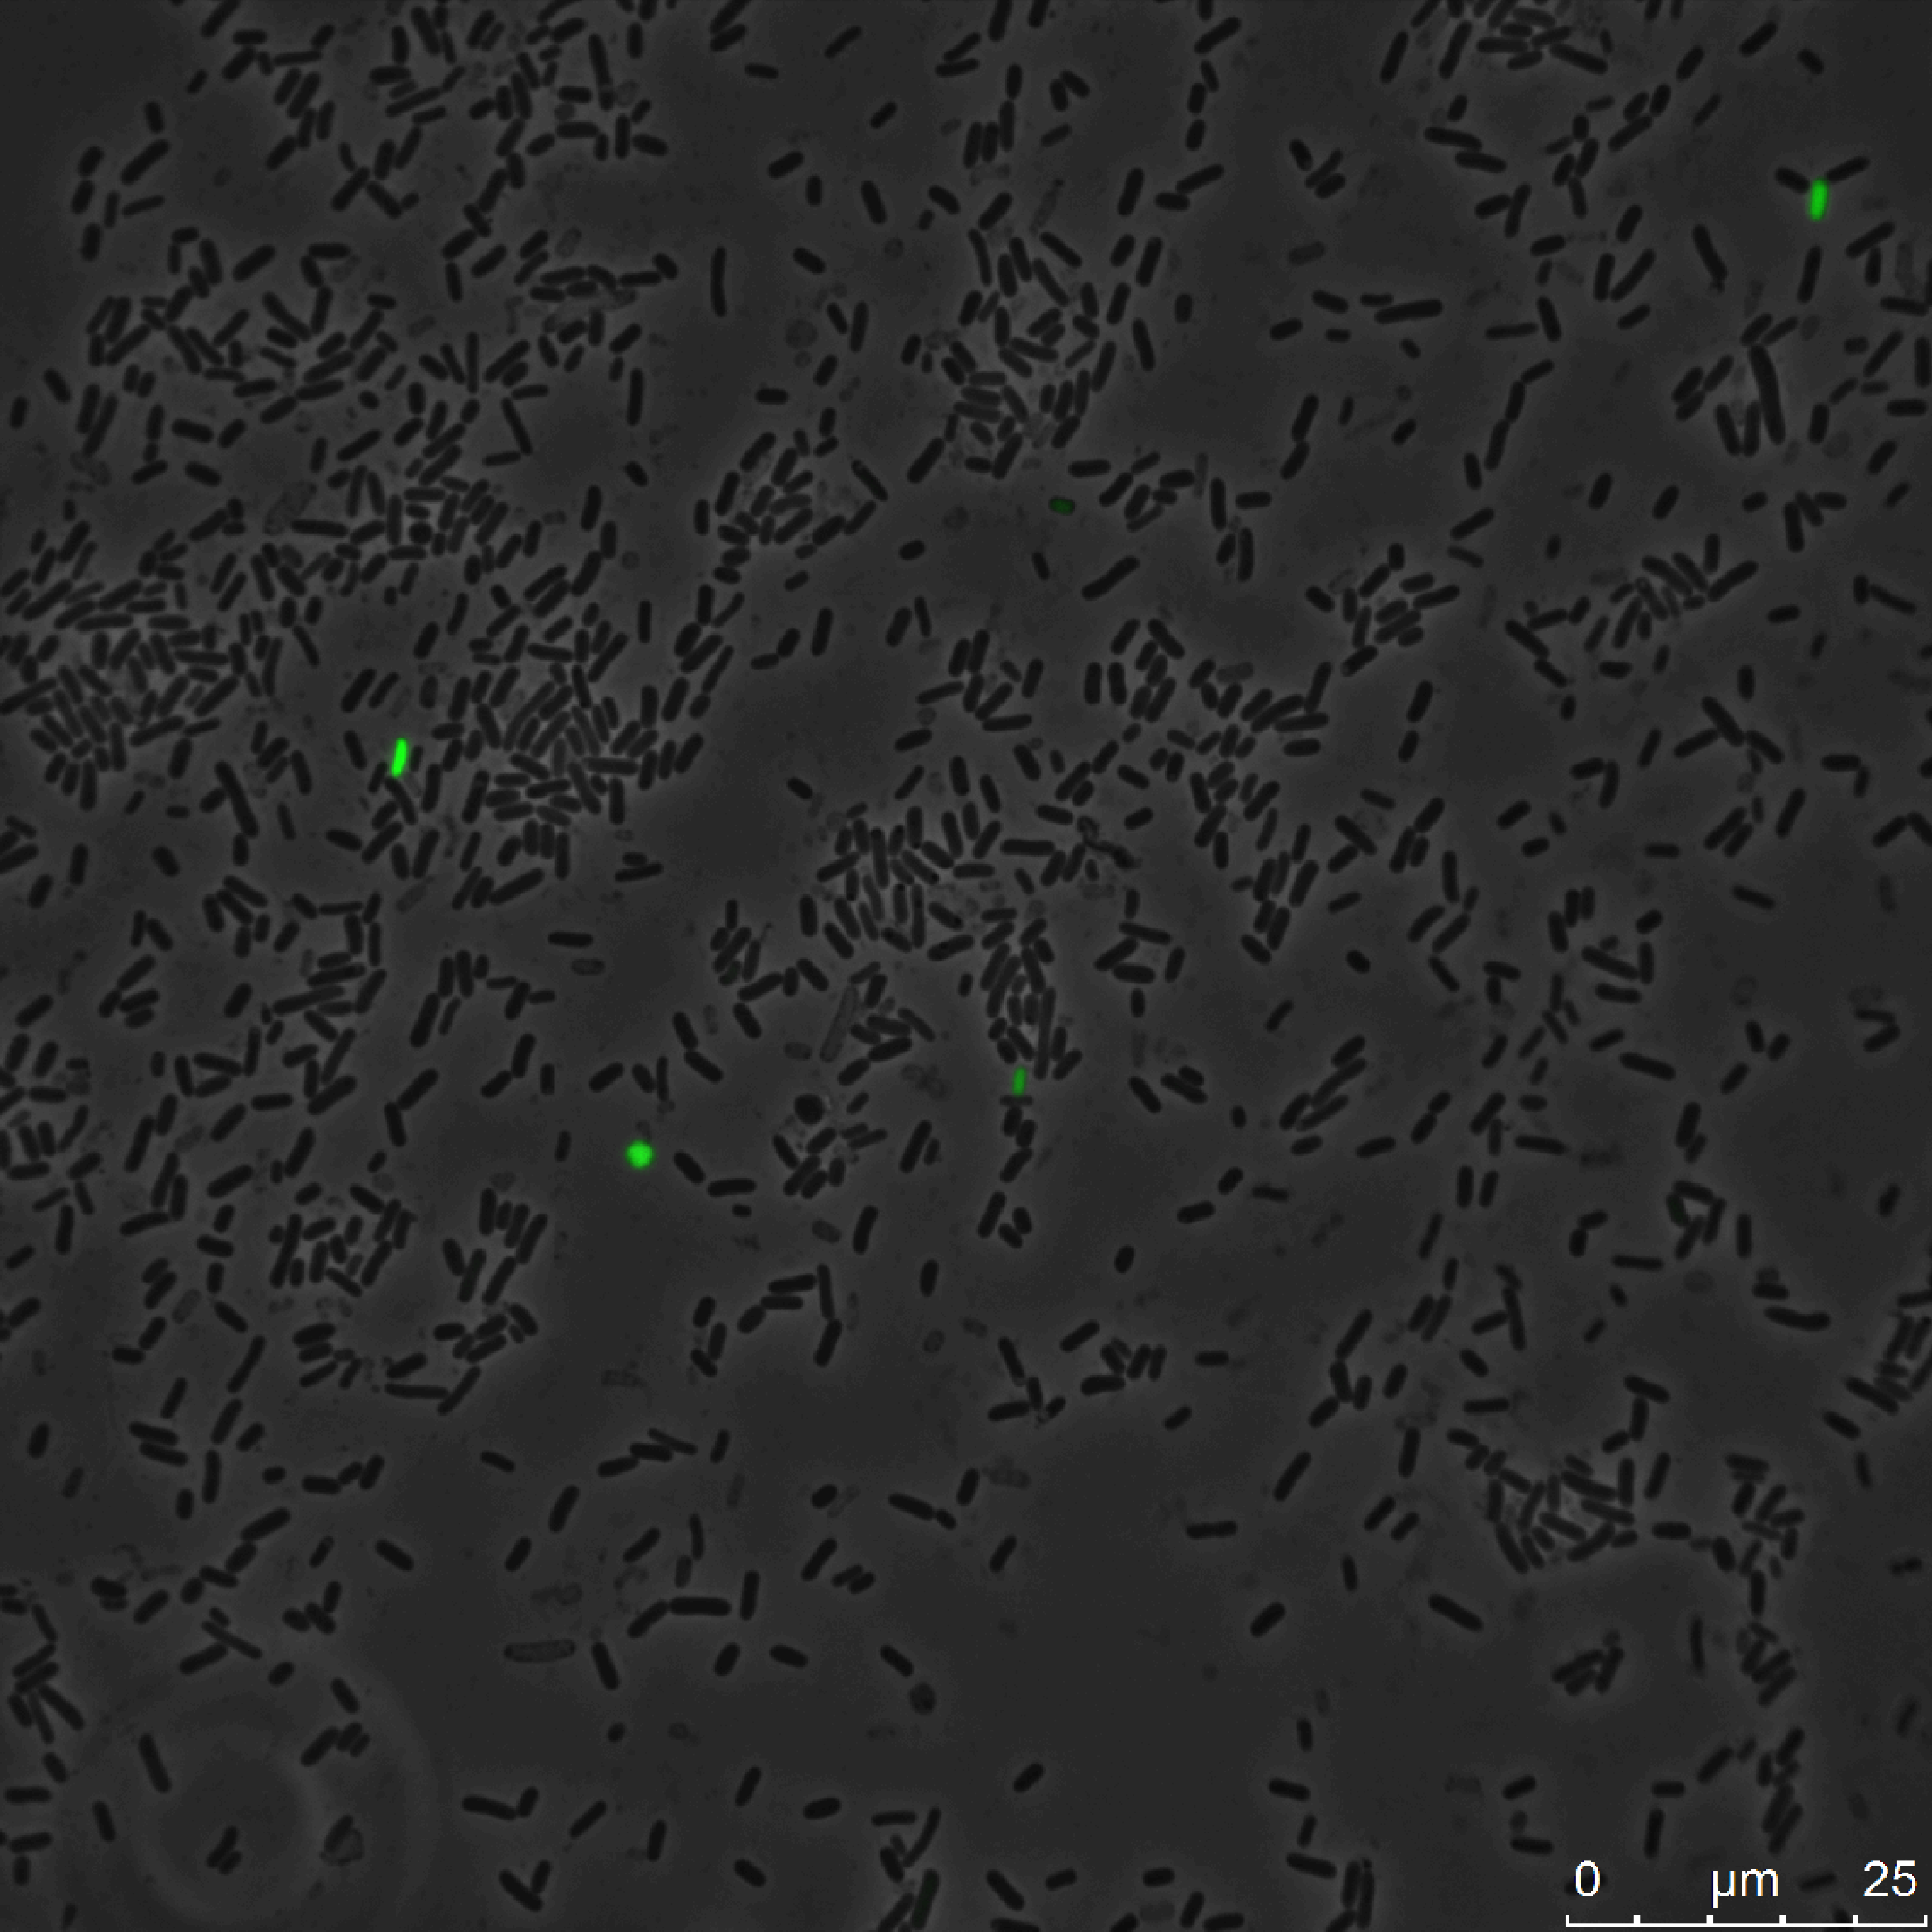
\includegraphics{THAIU1_24HR_8_GREEN.pdf} &%
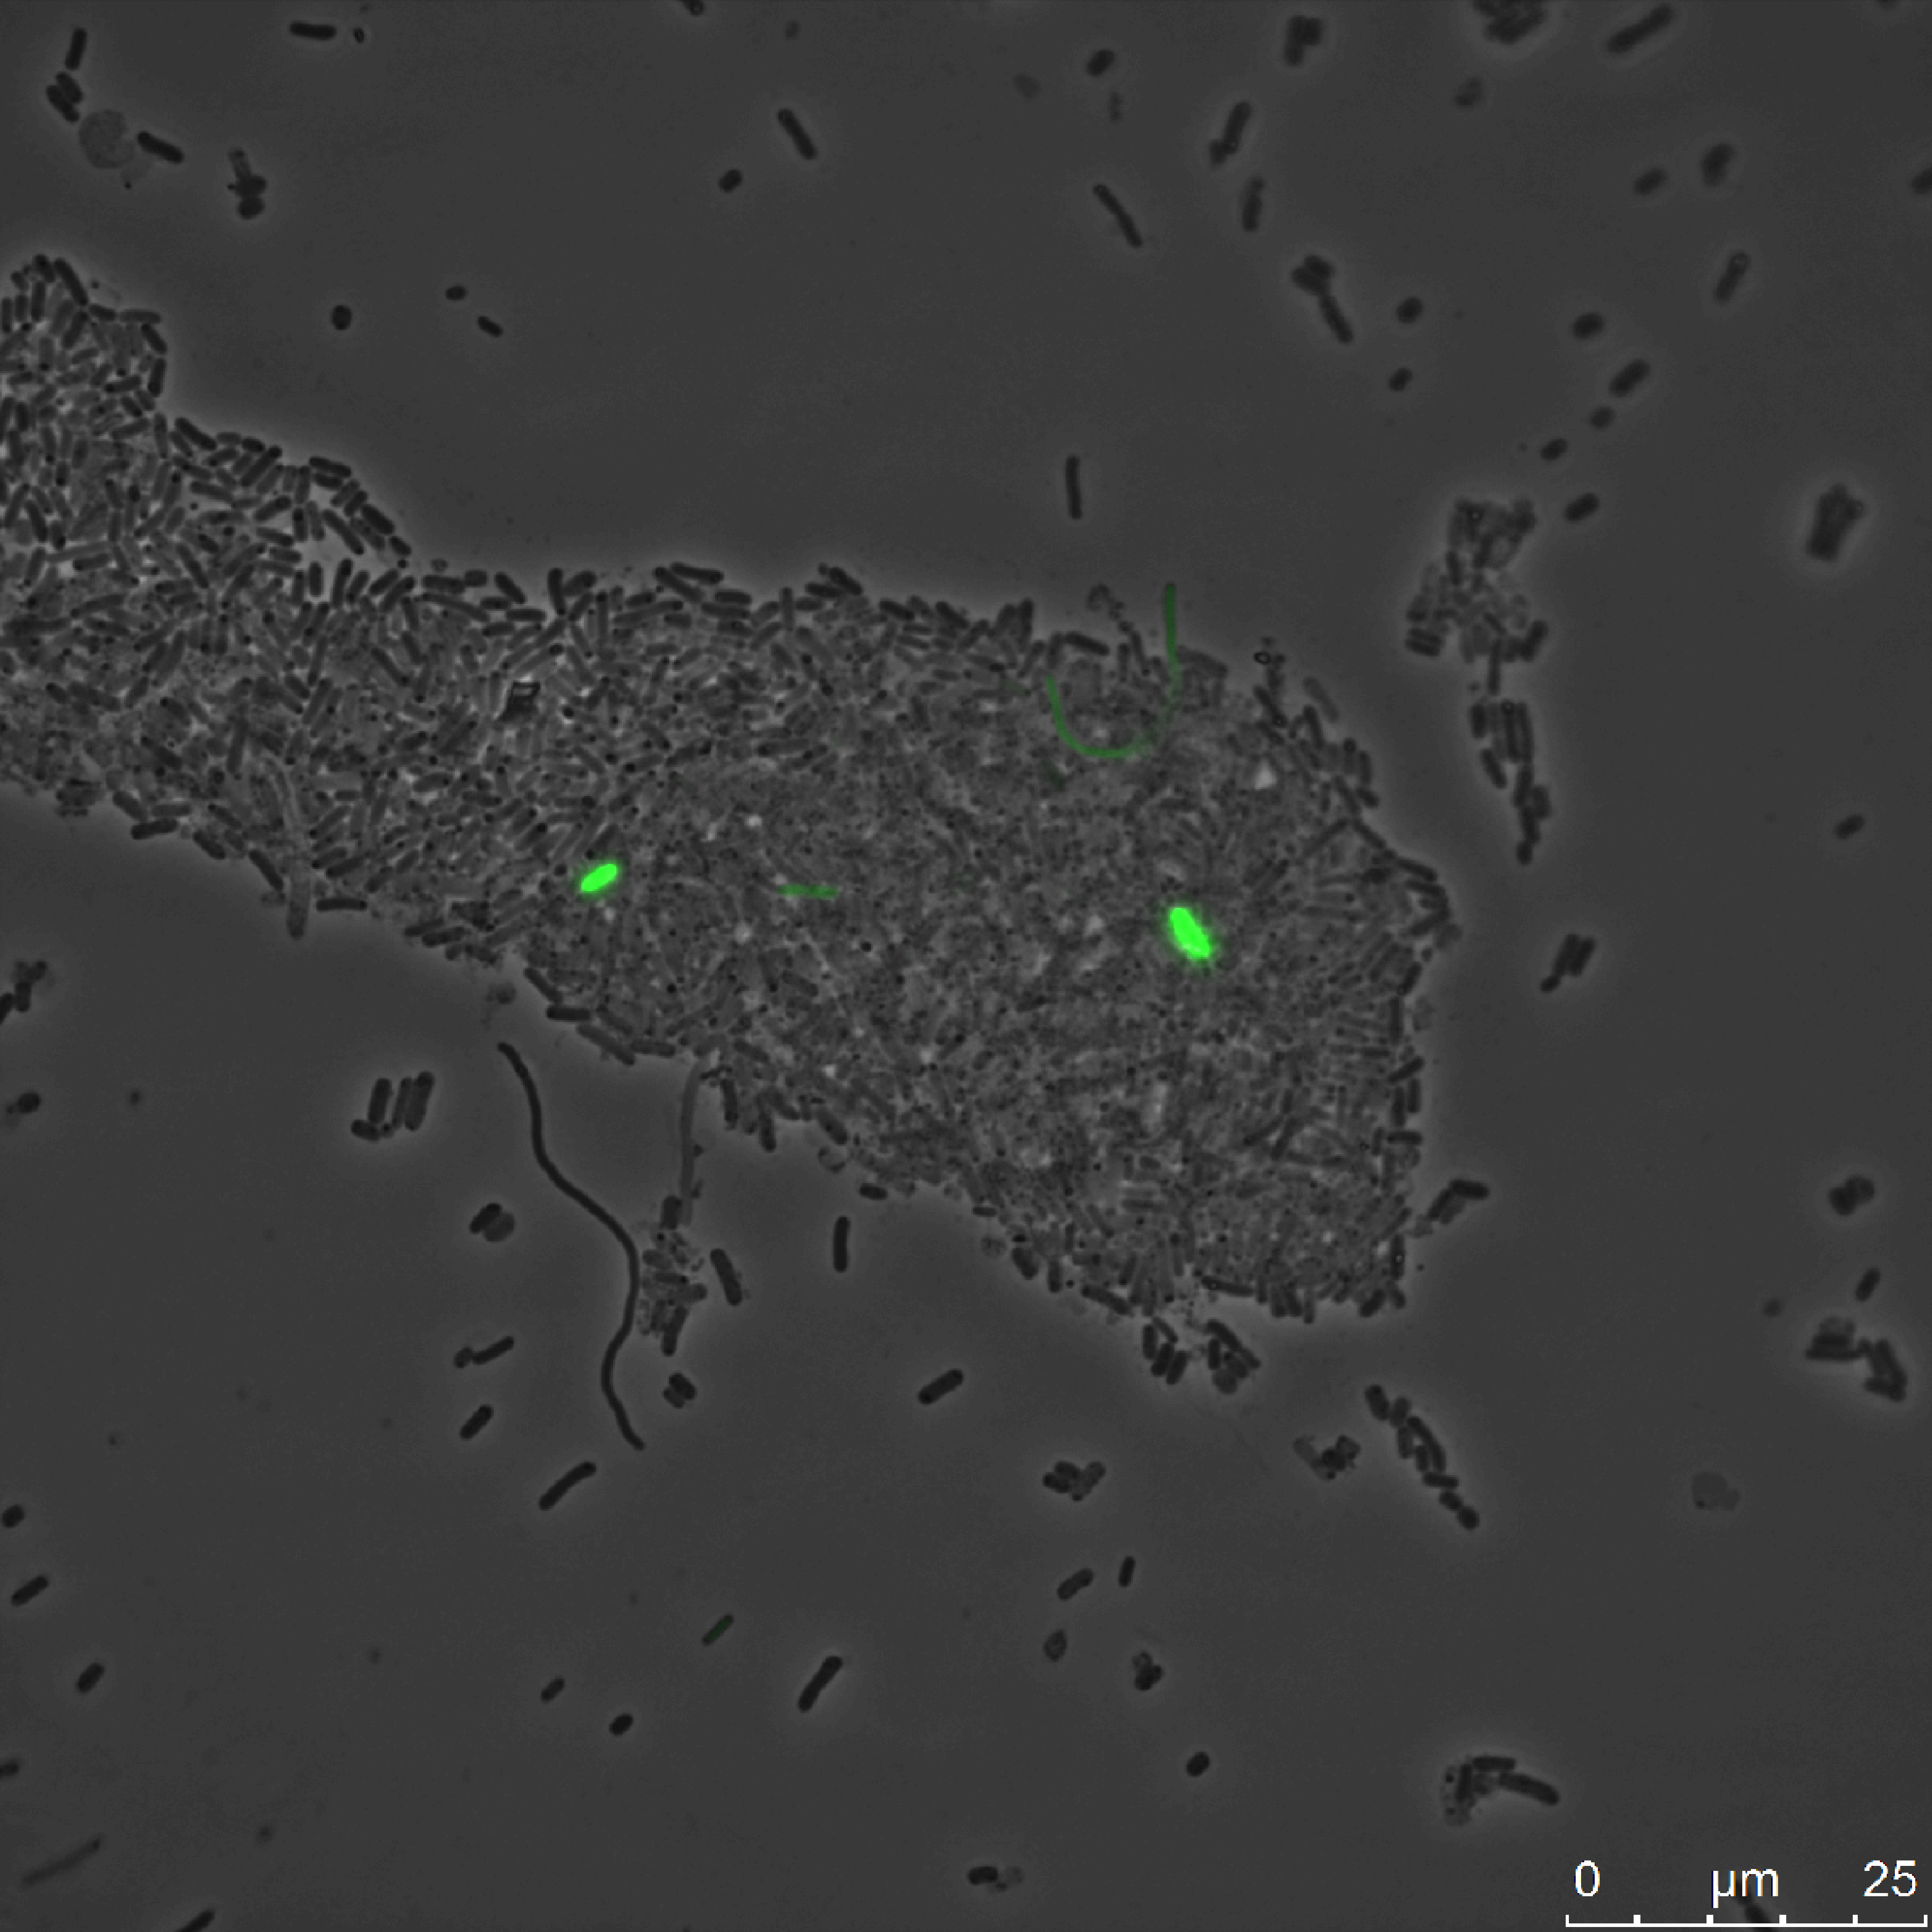
\includegraphics{THAIU1_72HR_4_GREEN.pdf} \\
 +++ & +++ & +++ & +++ \\[1ex]

\end{tabularx}

\label{RMTHAIU1}
\captionsetup{singlelinecheck=off, justification=justified, font=footnotesize, aboveskip=20pt}
\caption[Reporter microscopy - PB68.1 Unit 1]{\textsc{\normalsize Reporter microscopy for the \emph{P. asymbiotica} PB68.1 ``Unit 1" promoter.}\vspace{0.1cm} \newline A representative selection of images for 4 time points, for the PVC ``Unit 1" promoter fusion. Quadruplicate images are displayed vertically as representative of the whole slide sample. Key to qualitative fluorescence indication: ``-" - no fluorescence, ``+" - low level fluorescence in isolated cells. ``++" - low level fluorescence in many cells or few brighter cells, ``+++" - intermediate to high fluorescence in almost all cells, or very bright isolated cells.}
\end{figure}
\endgroup

%%%%%%%%%%%%%%%%%%%%%%%%%%%%%%%%%%%%%%%%%%%%%%%%%%%%%%%%%%%%%%%%%%%%

\begingroup
\renewcommand{\arraystretch}{0.8}%
\setlength{\tabcolsep}{0.3pt}
\begin{figure}[p]
\setkeys{Gin}{width=\linewidth}
\Huge
\begin{tabularx}{\textwidth}{CCCC}
\multicolumn{4}{p{\linewidth}}{\large \centering \textbf{\emph{P. luminescens} TT01 PVC ``Unit 4"}} \\
\hiderowcolors
& & & \\[-1.5ex]
\Large 2 Hours &\Large 5 Hours &\Large 24 Hours &\Large 72 Hours \\[1ex]

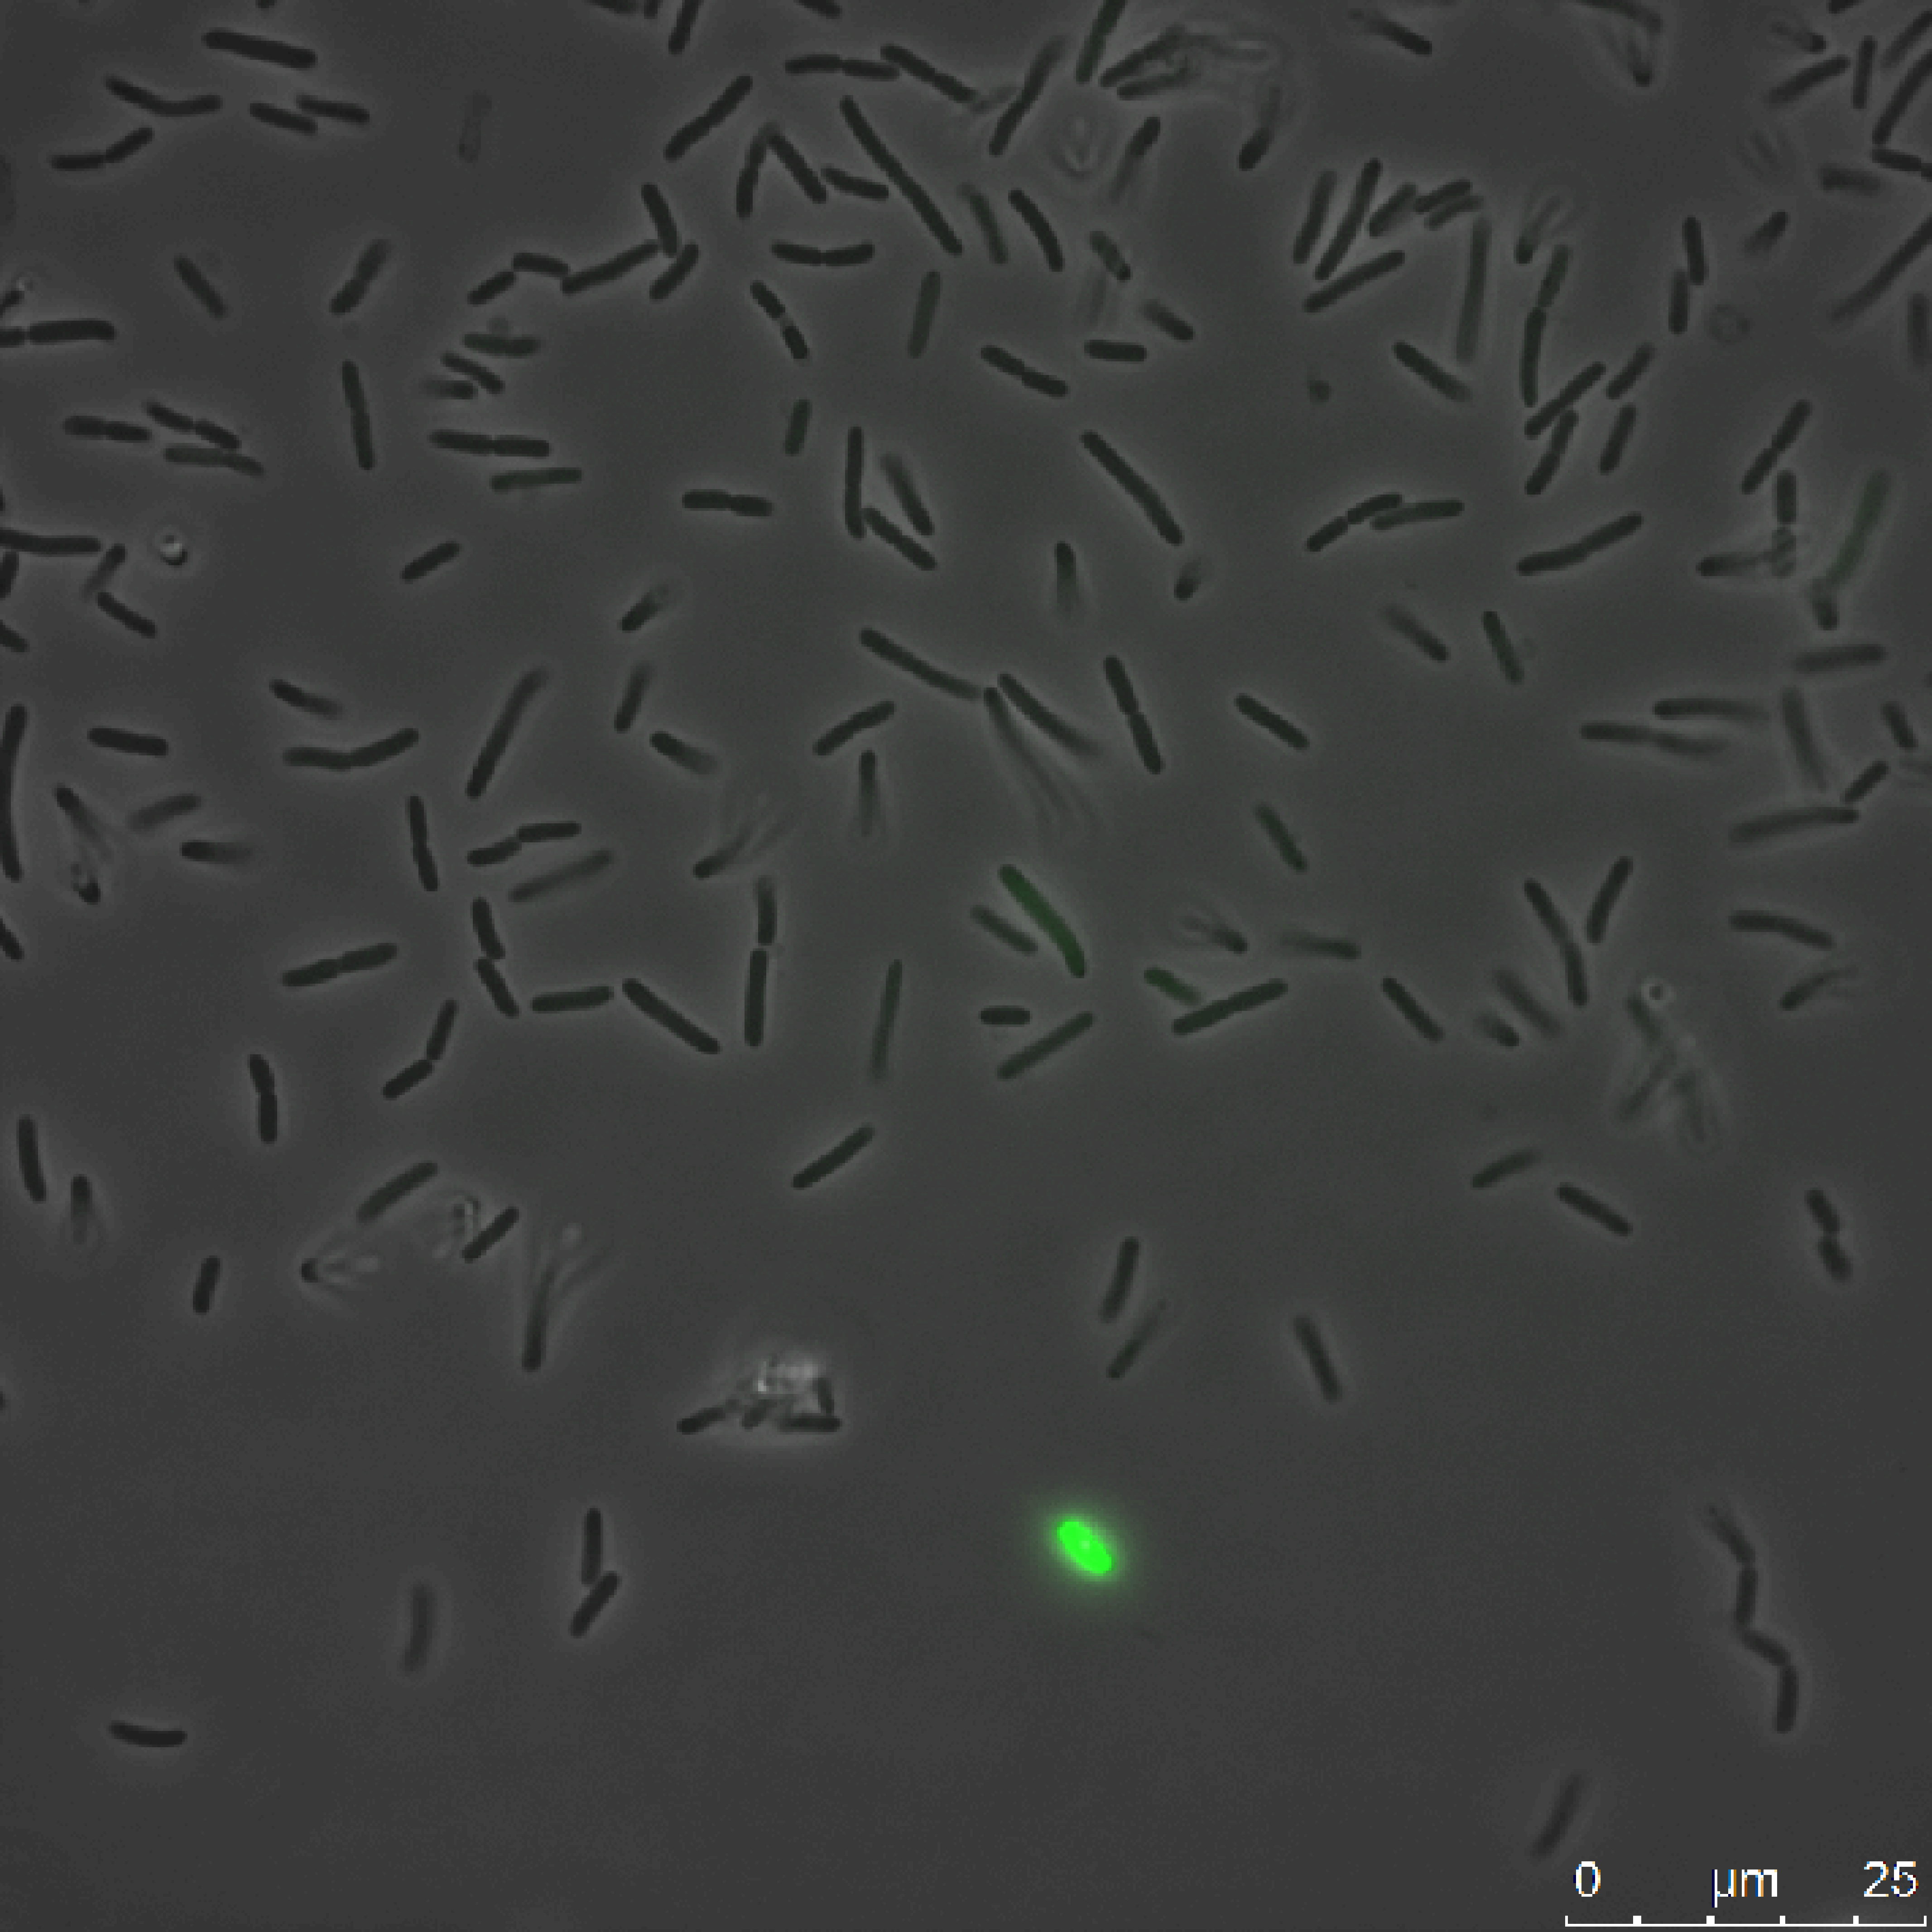
\includegraphics{TT01U4_1_GREEN.pdf} &%
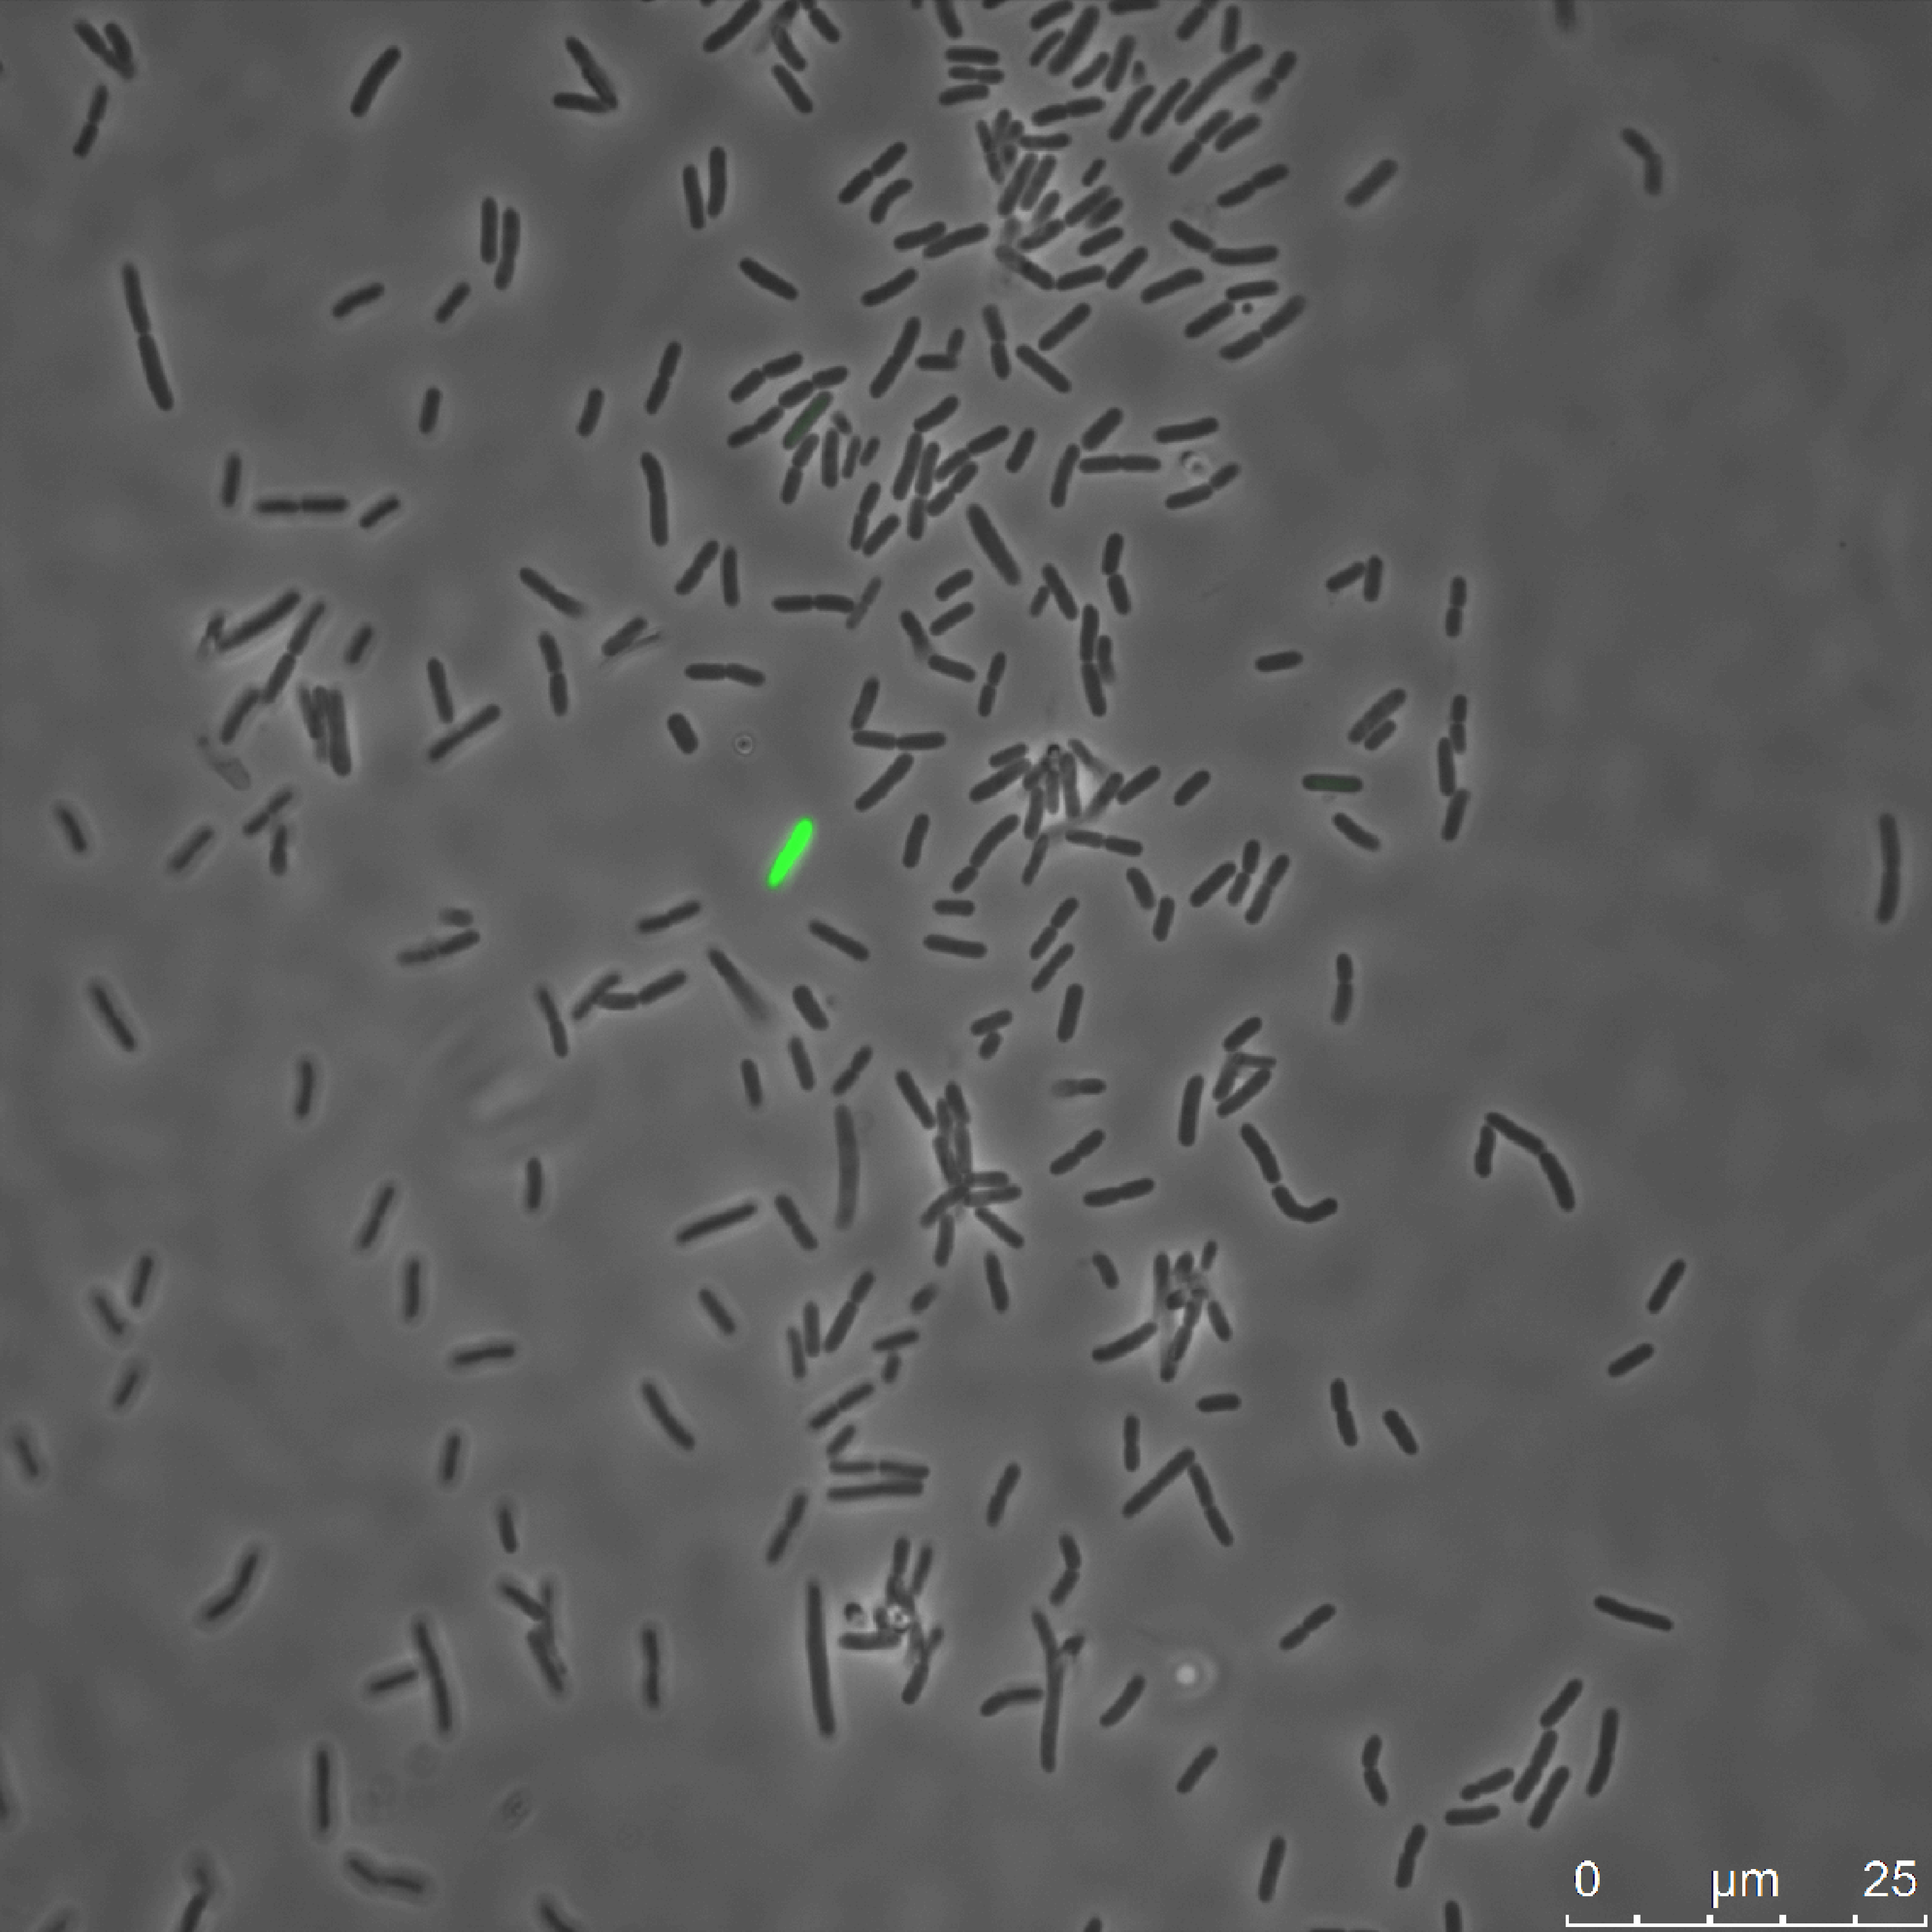
\includegraphics{TT01U4_5HR_1_GREEN.pdf} &%
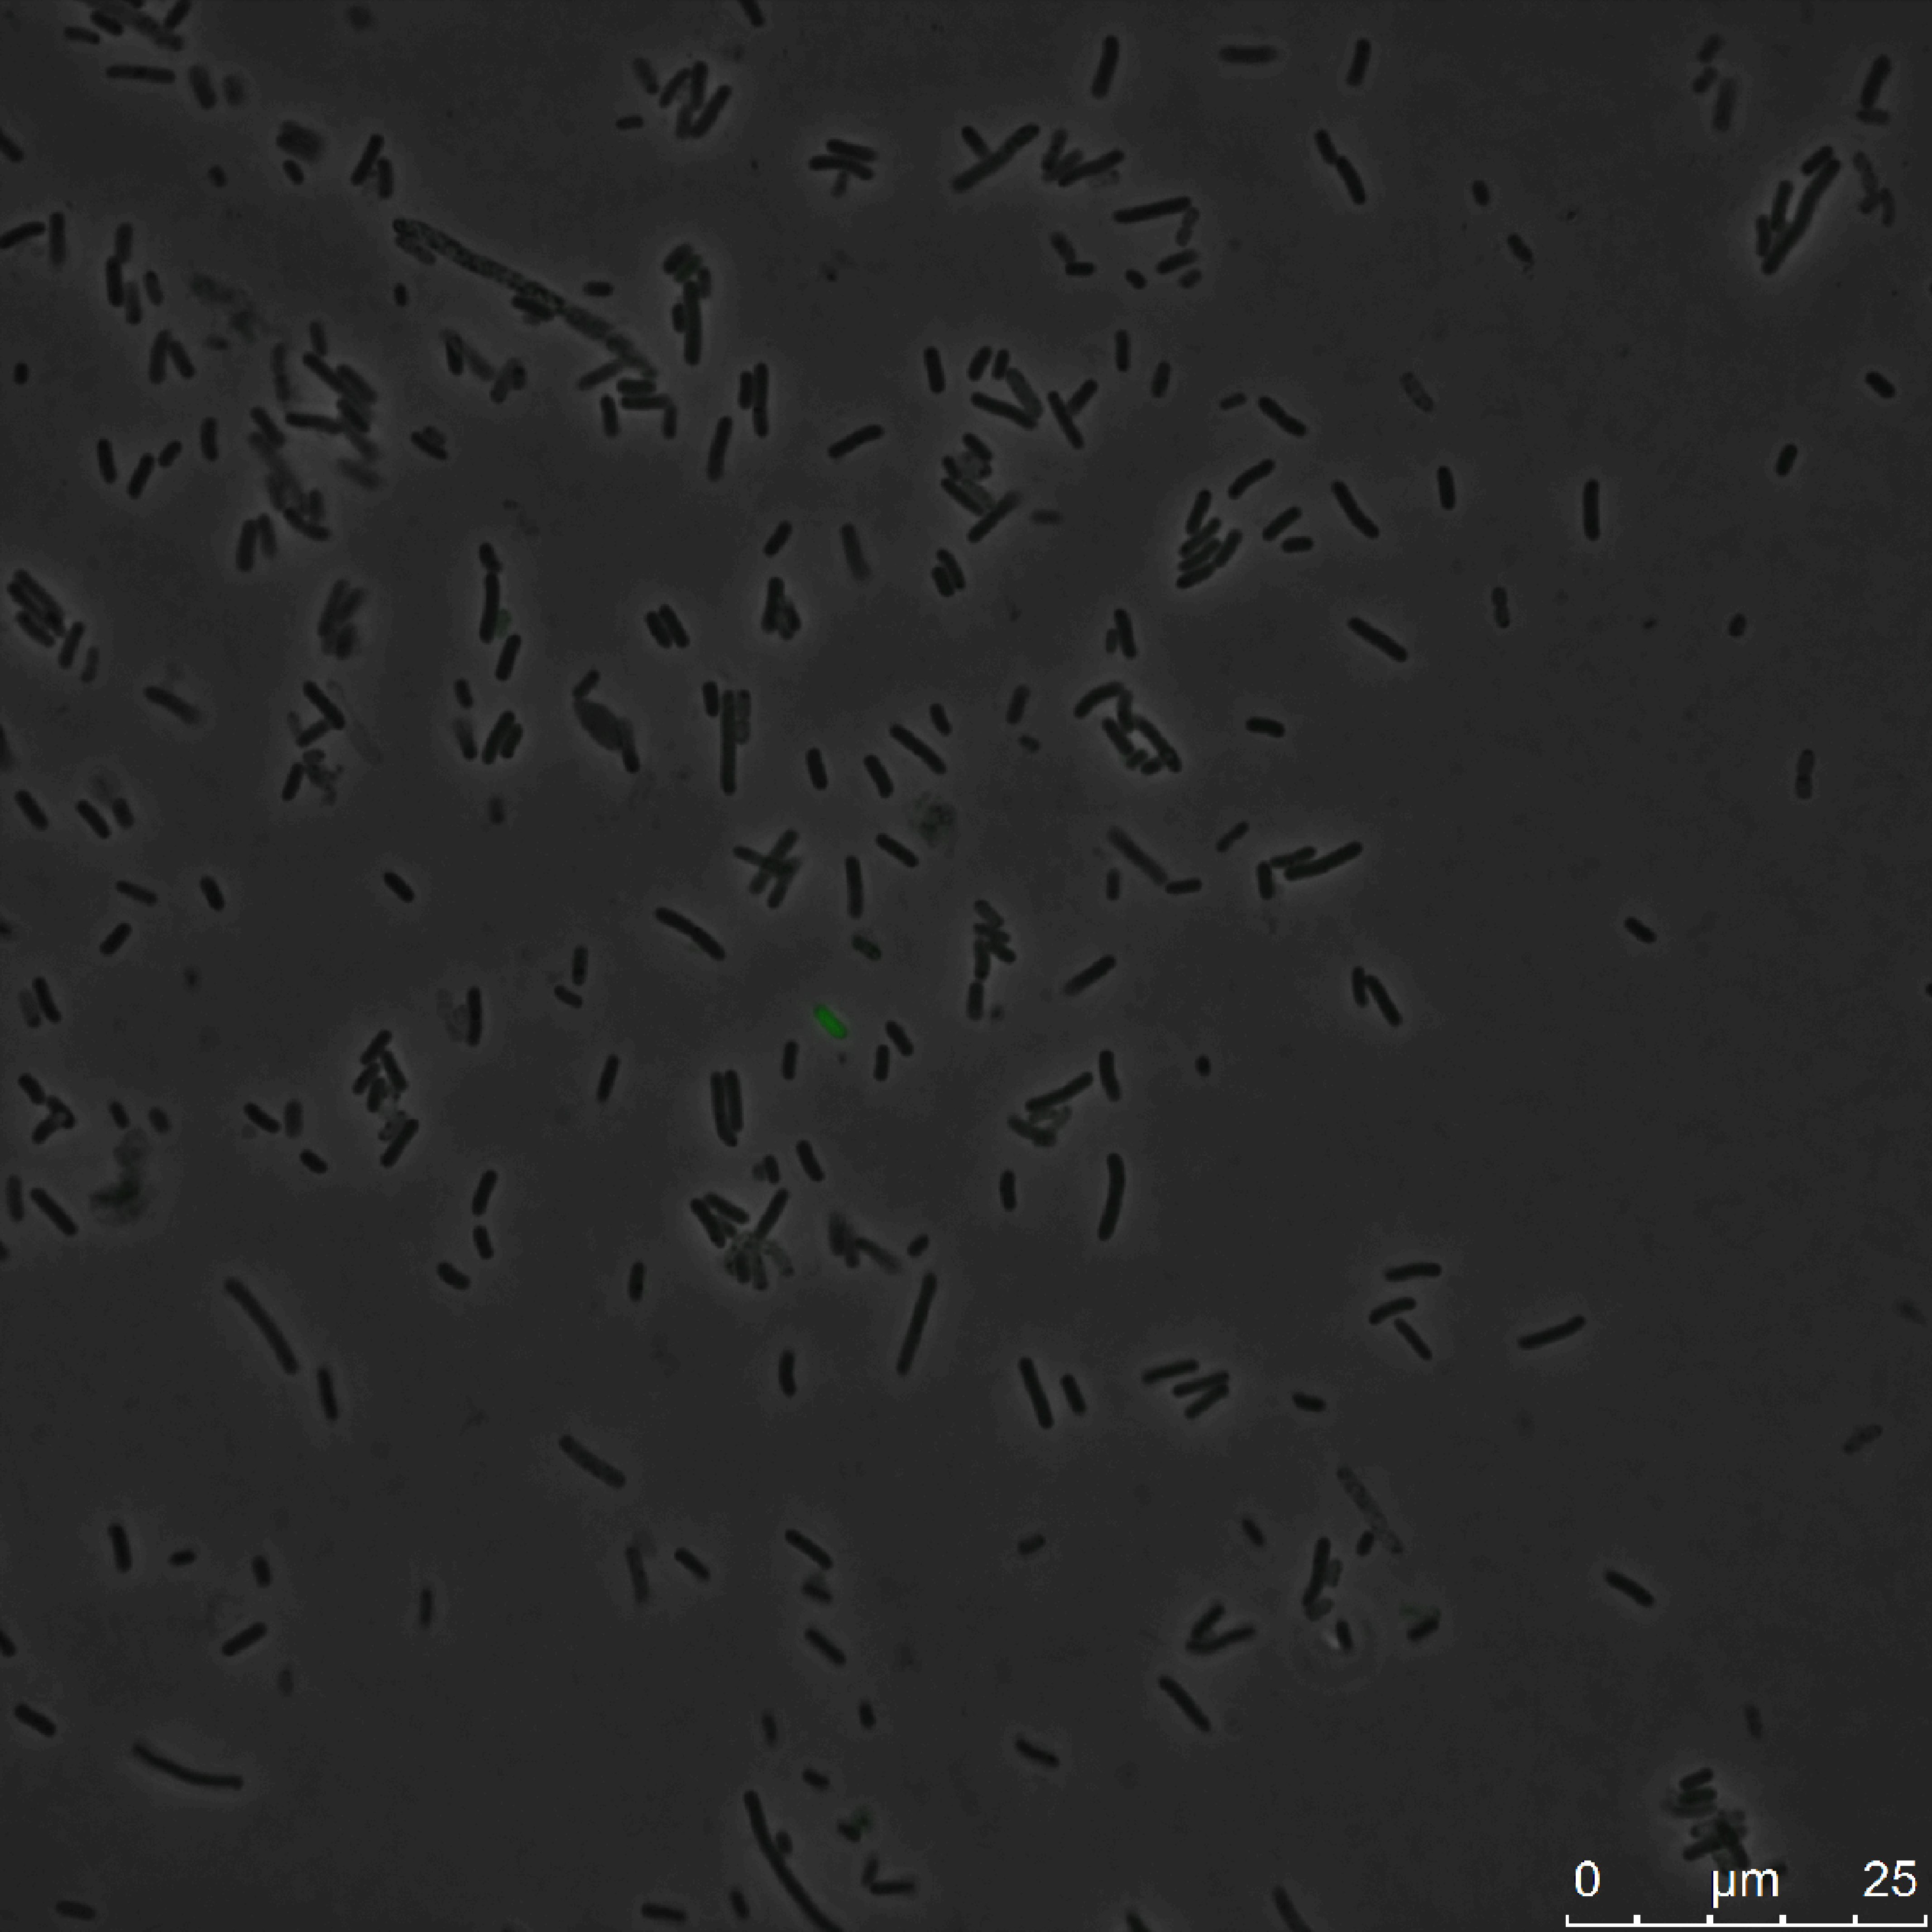
\includegraphics{TT01U4_24HR_1_GREEN.pdf} &%
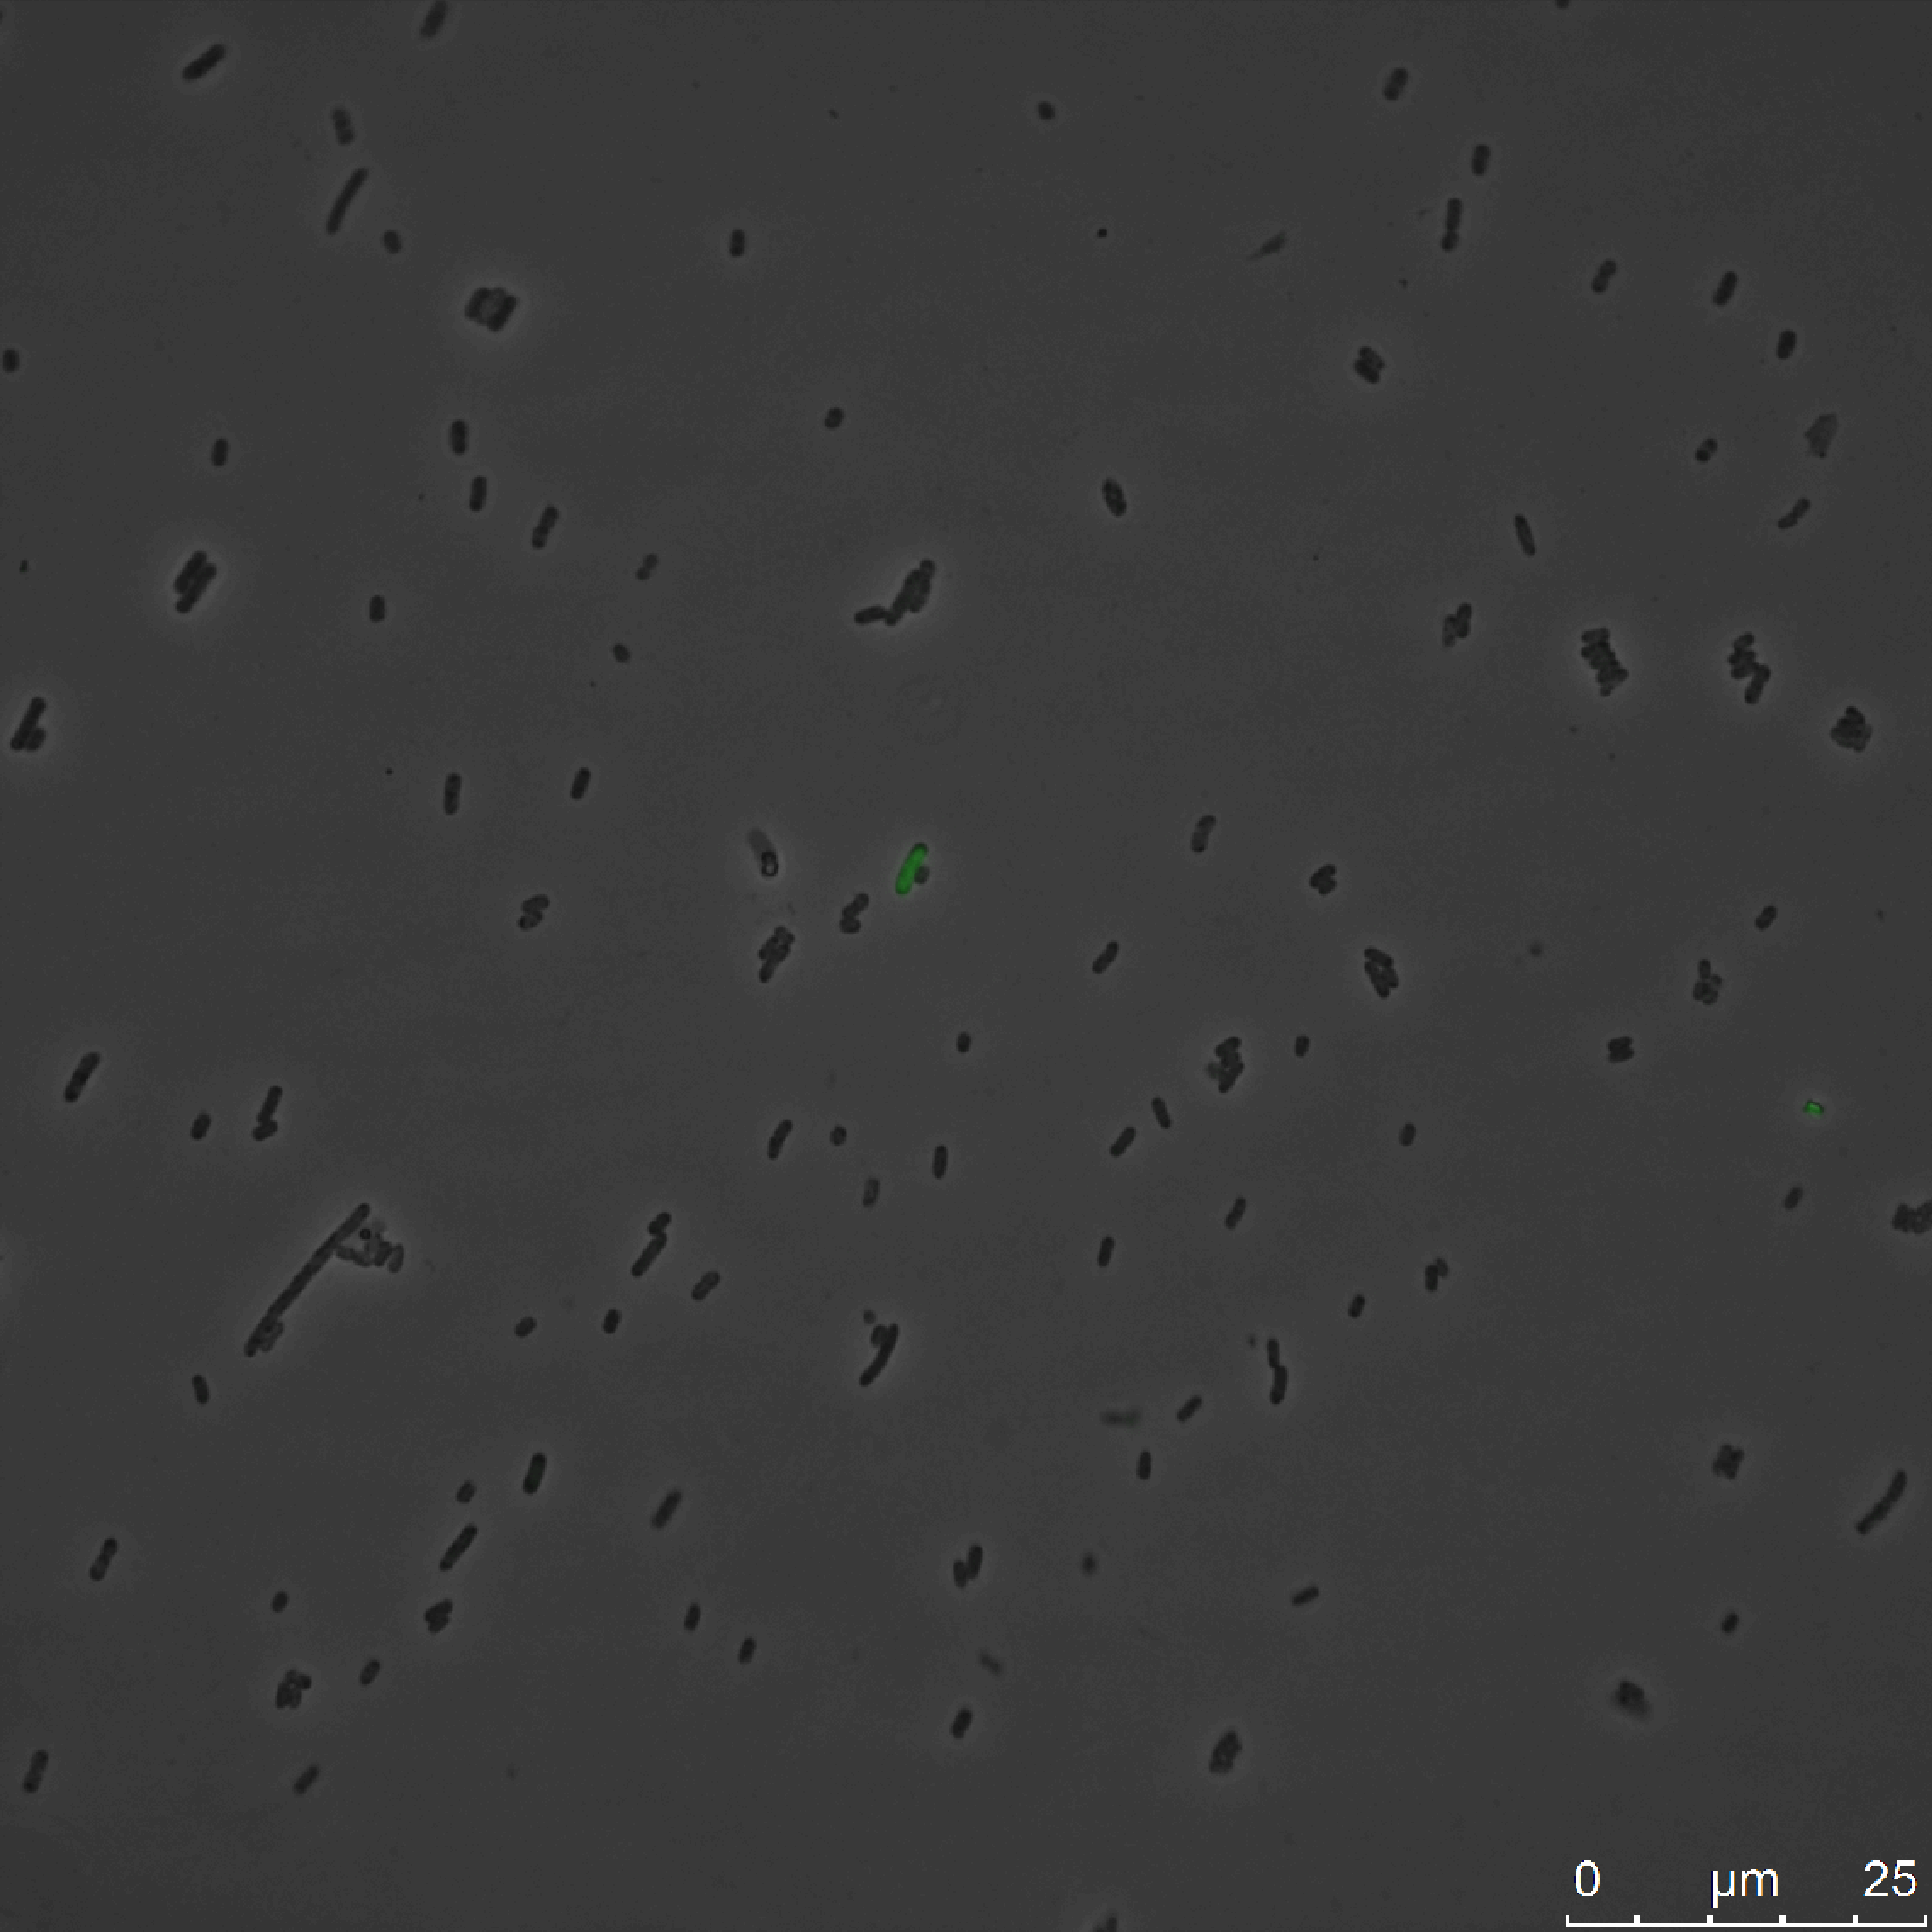
\includegraphics{TT01U4_72HR_1_GREEN.pdf} \\[-0.5ex]

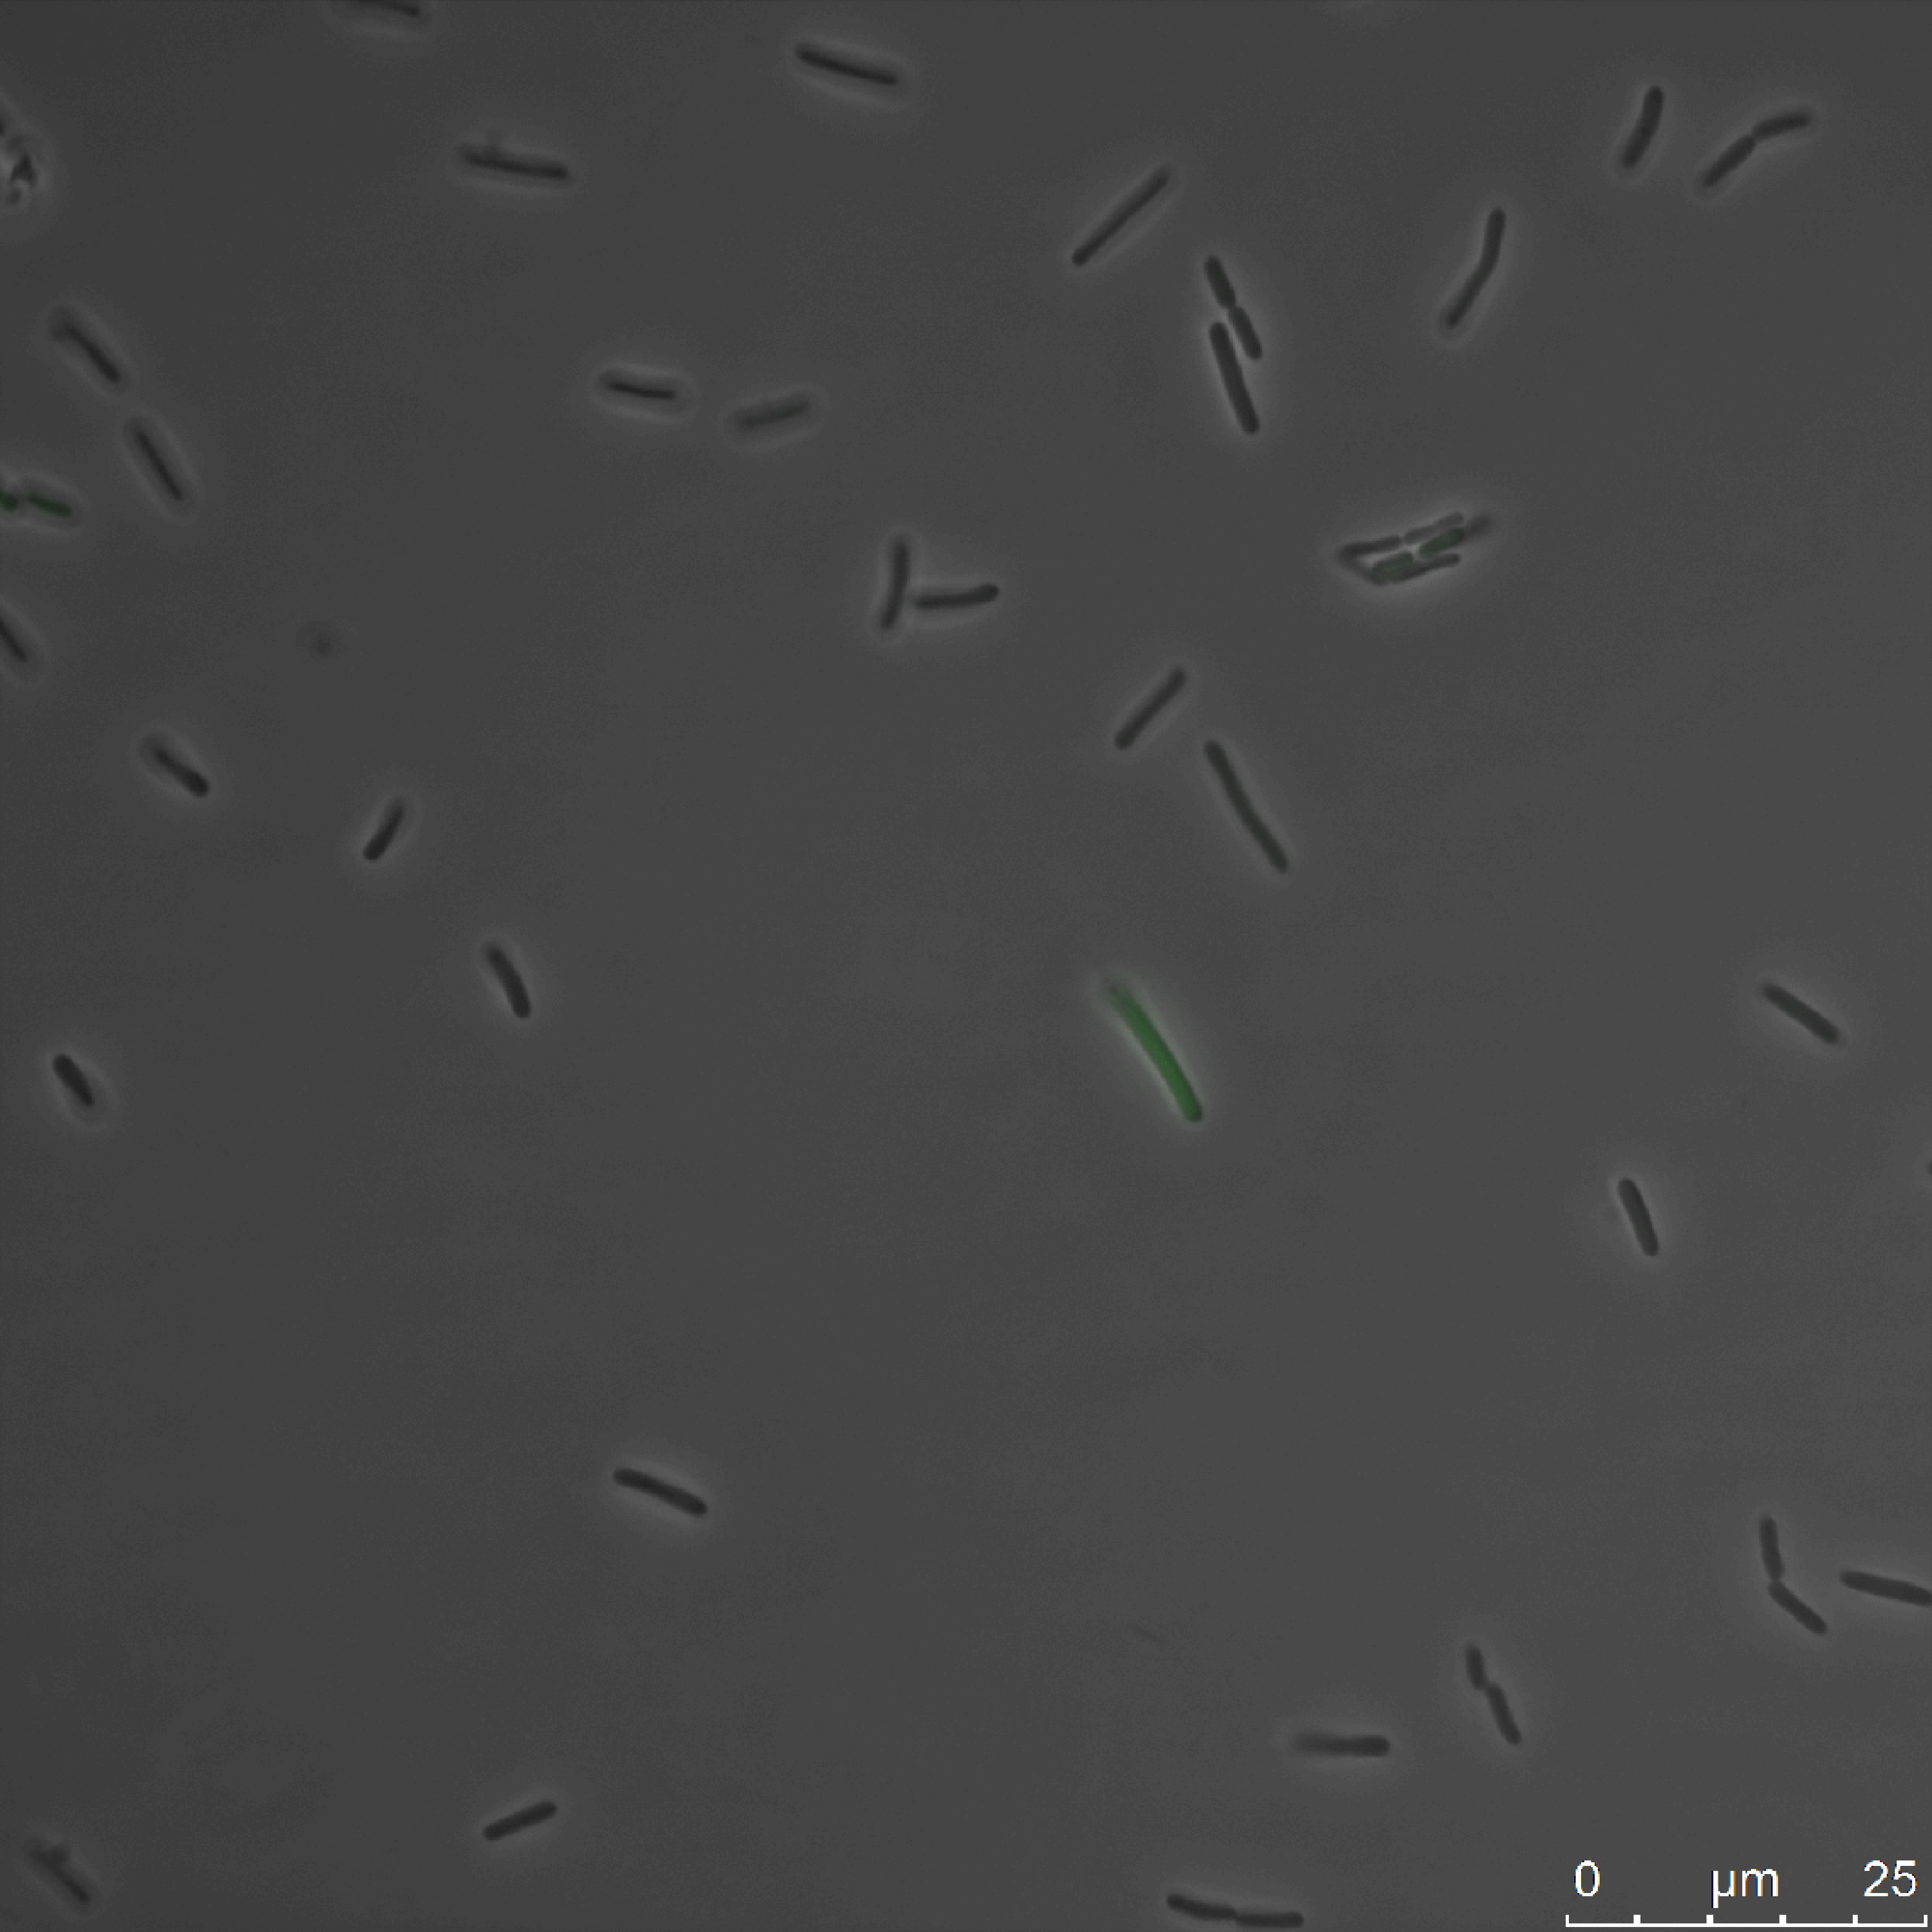
\includegraphics{TT01U4_2_GREEN.pdf} &%
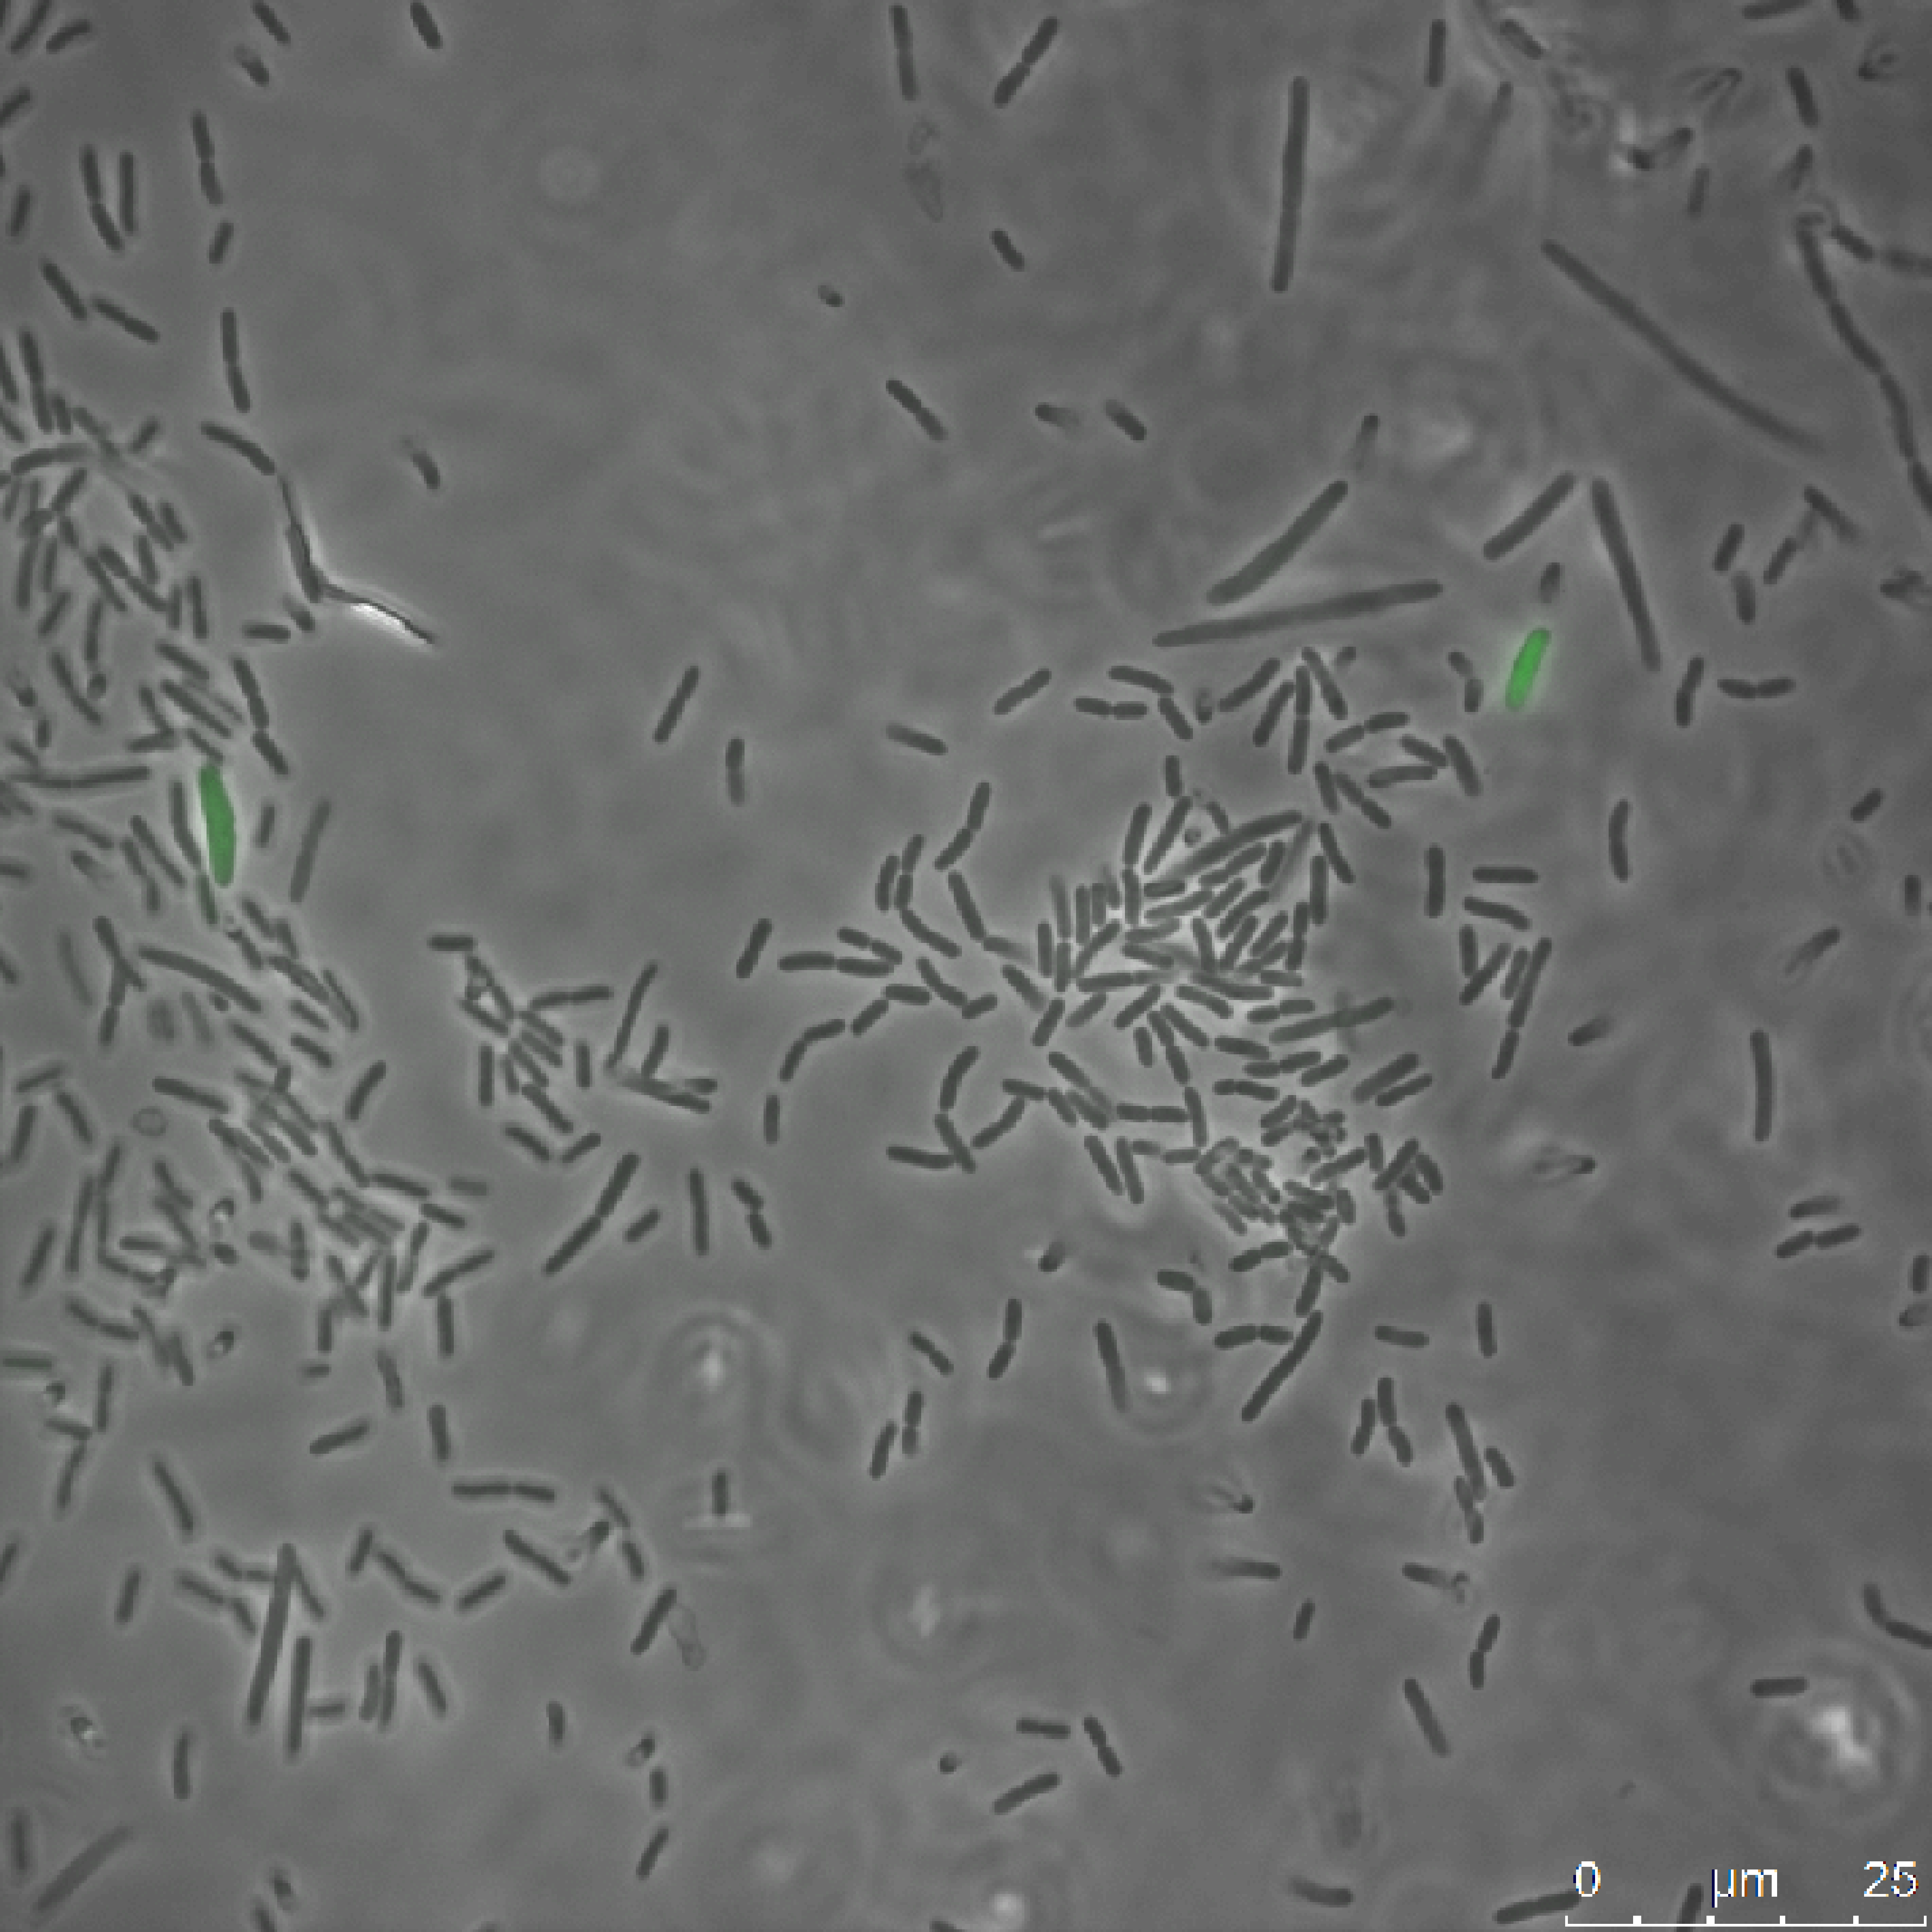
\includegraphics{TT01U4_5HR_2_GREEN.pdf} &%
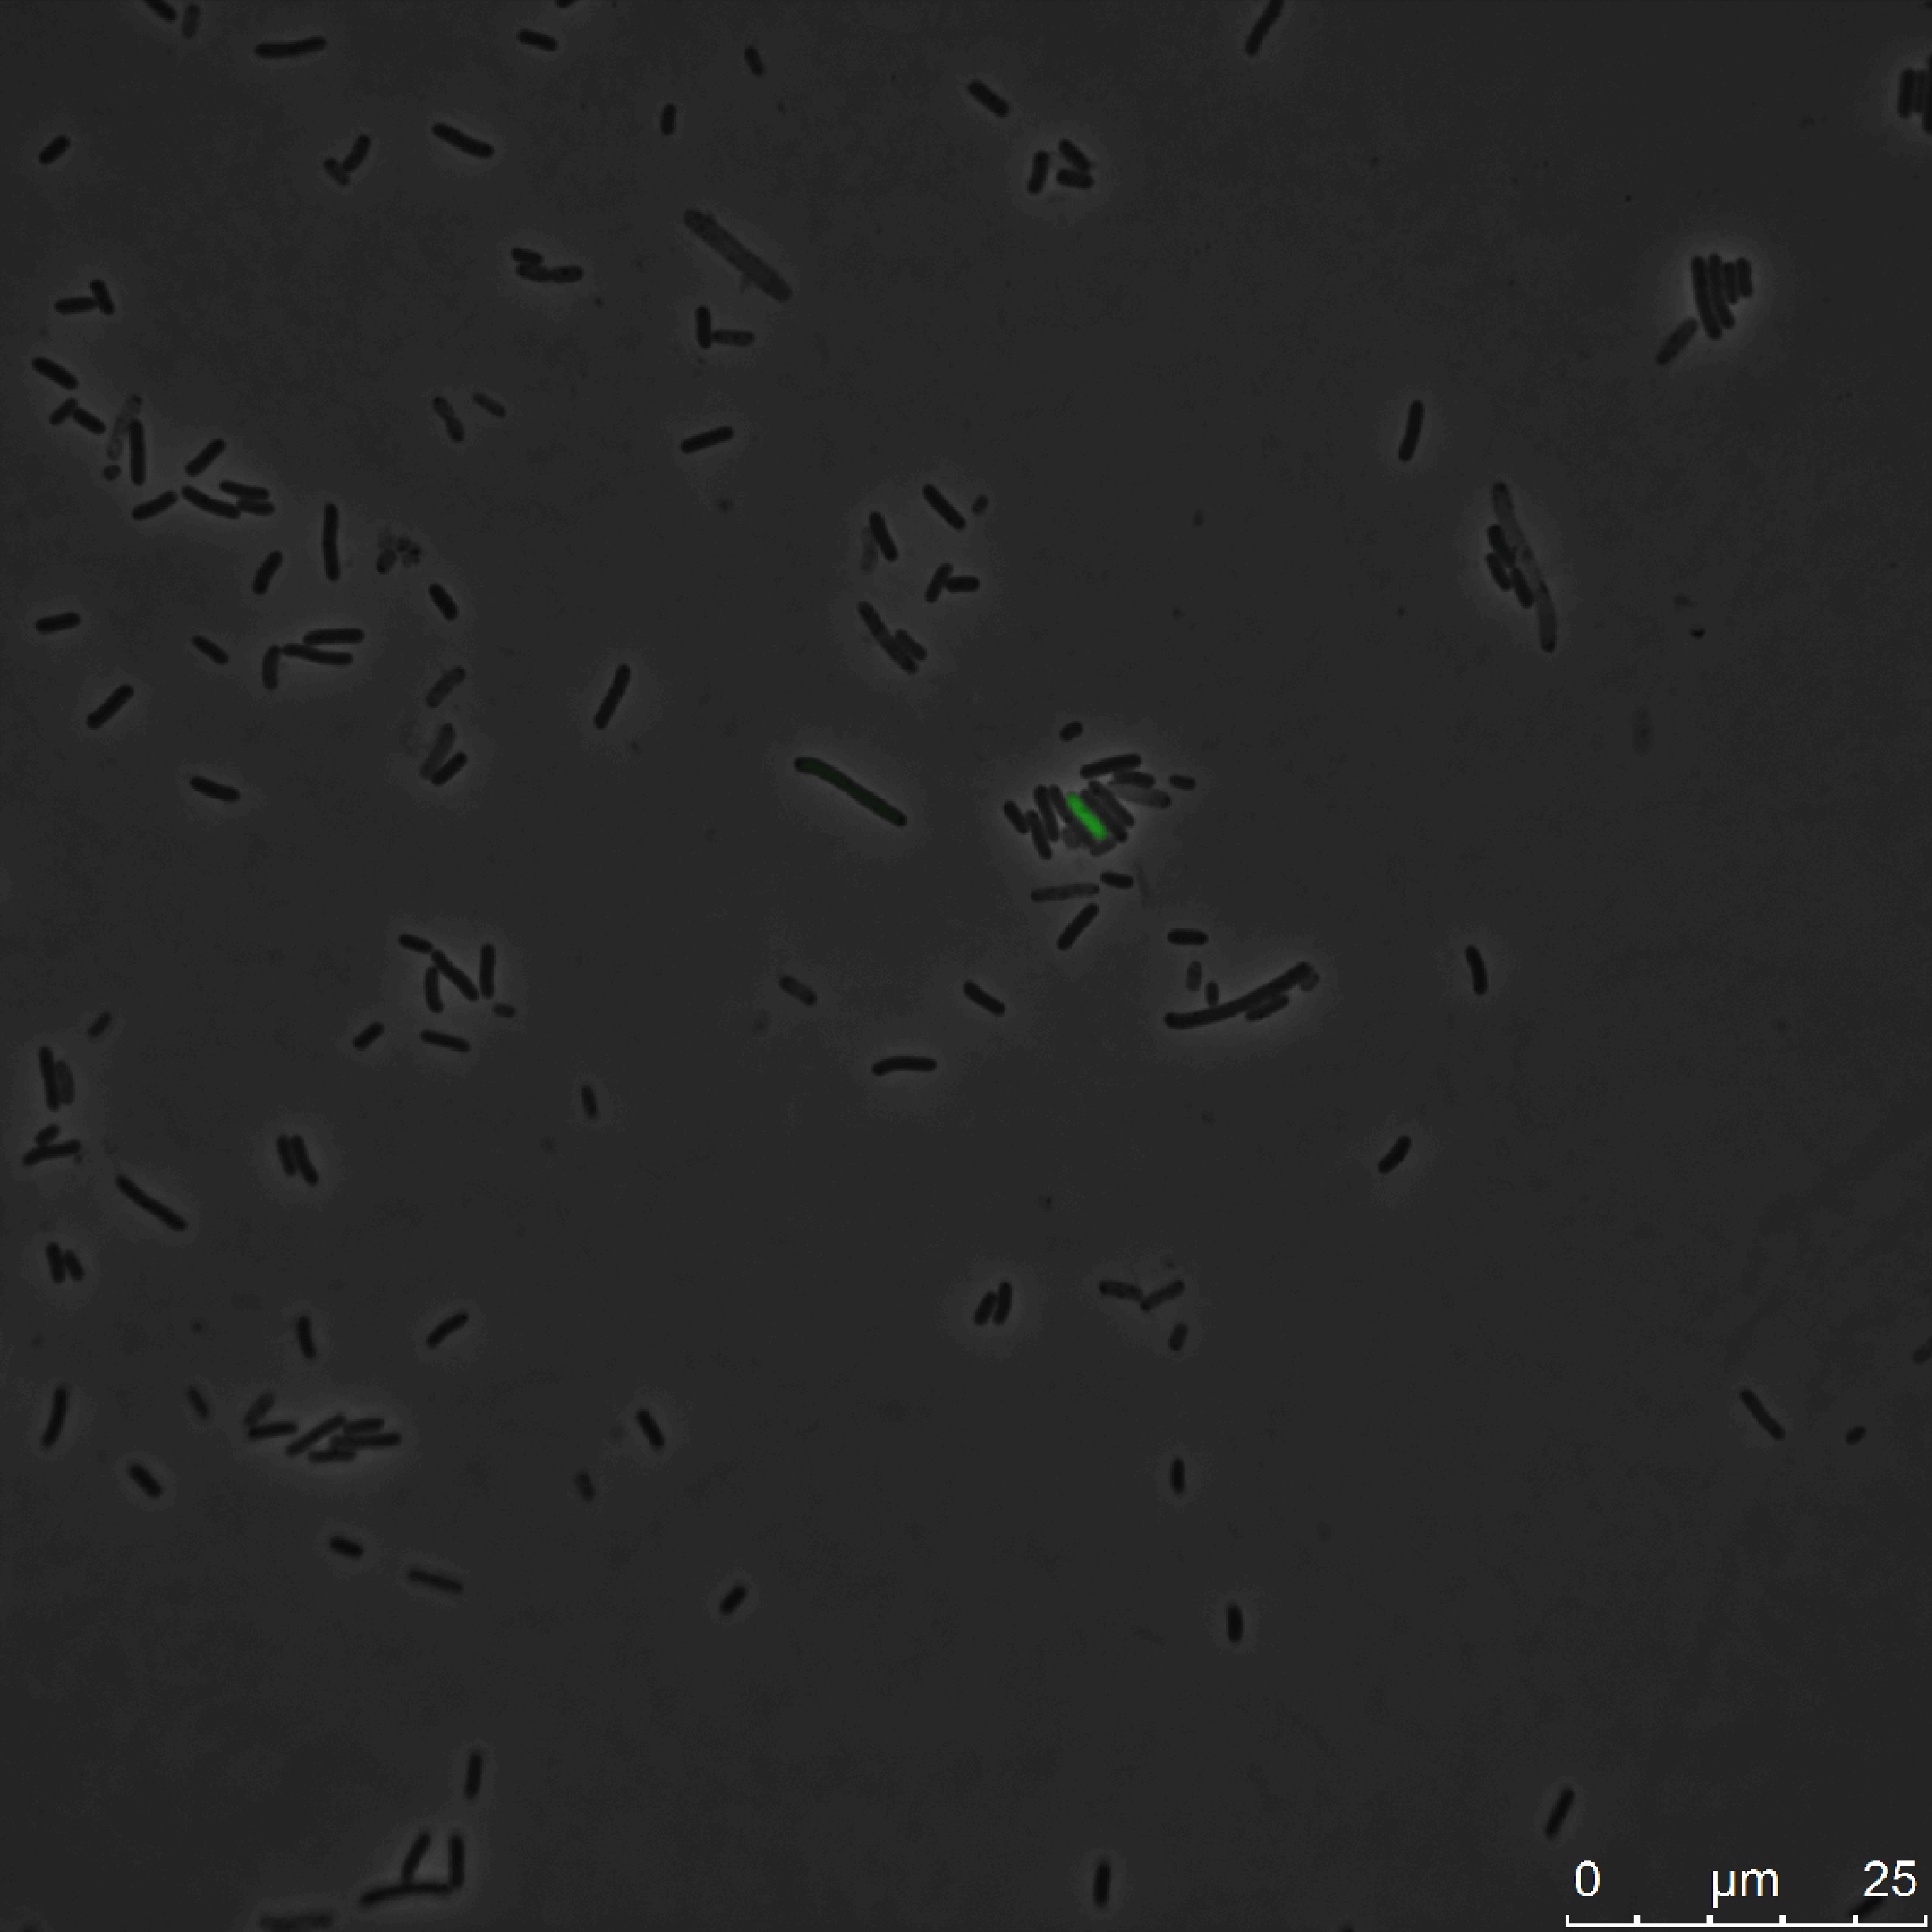
\includegraphics{TT01U4_24HR_2_GREEN.pdf} &%
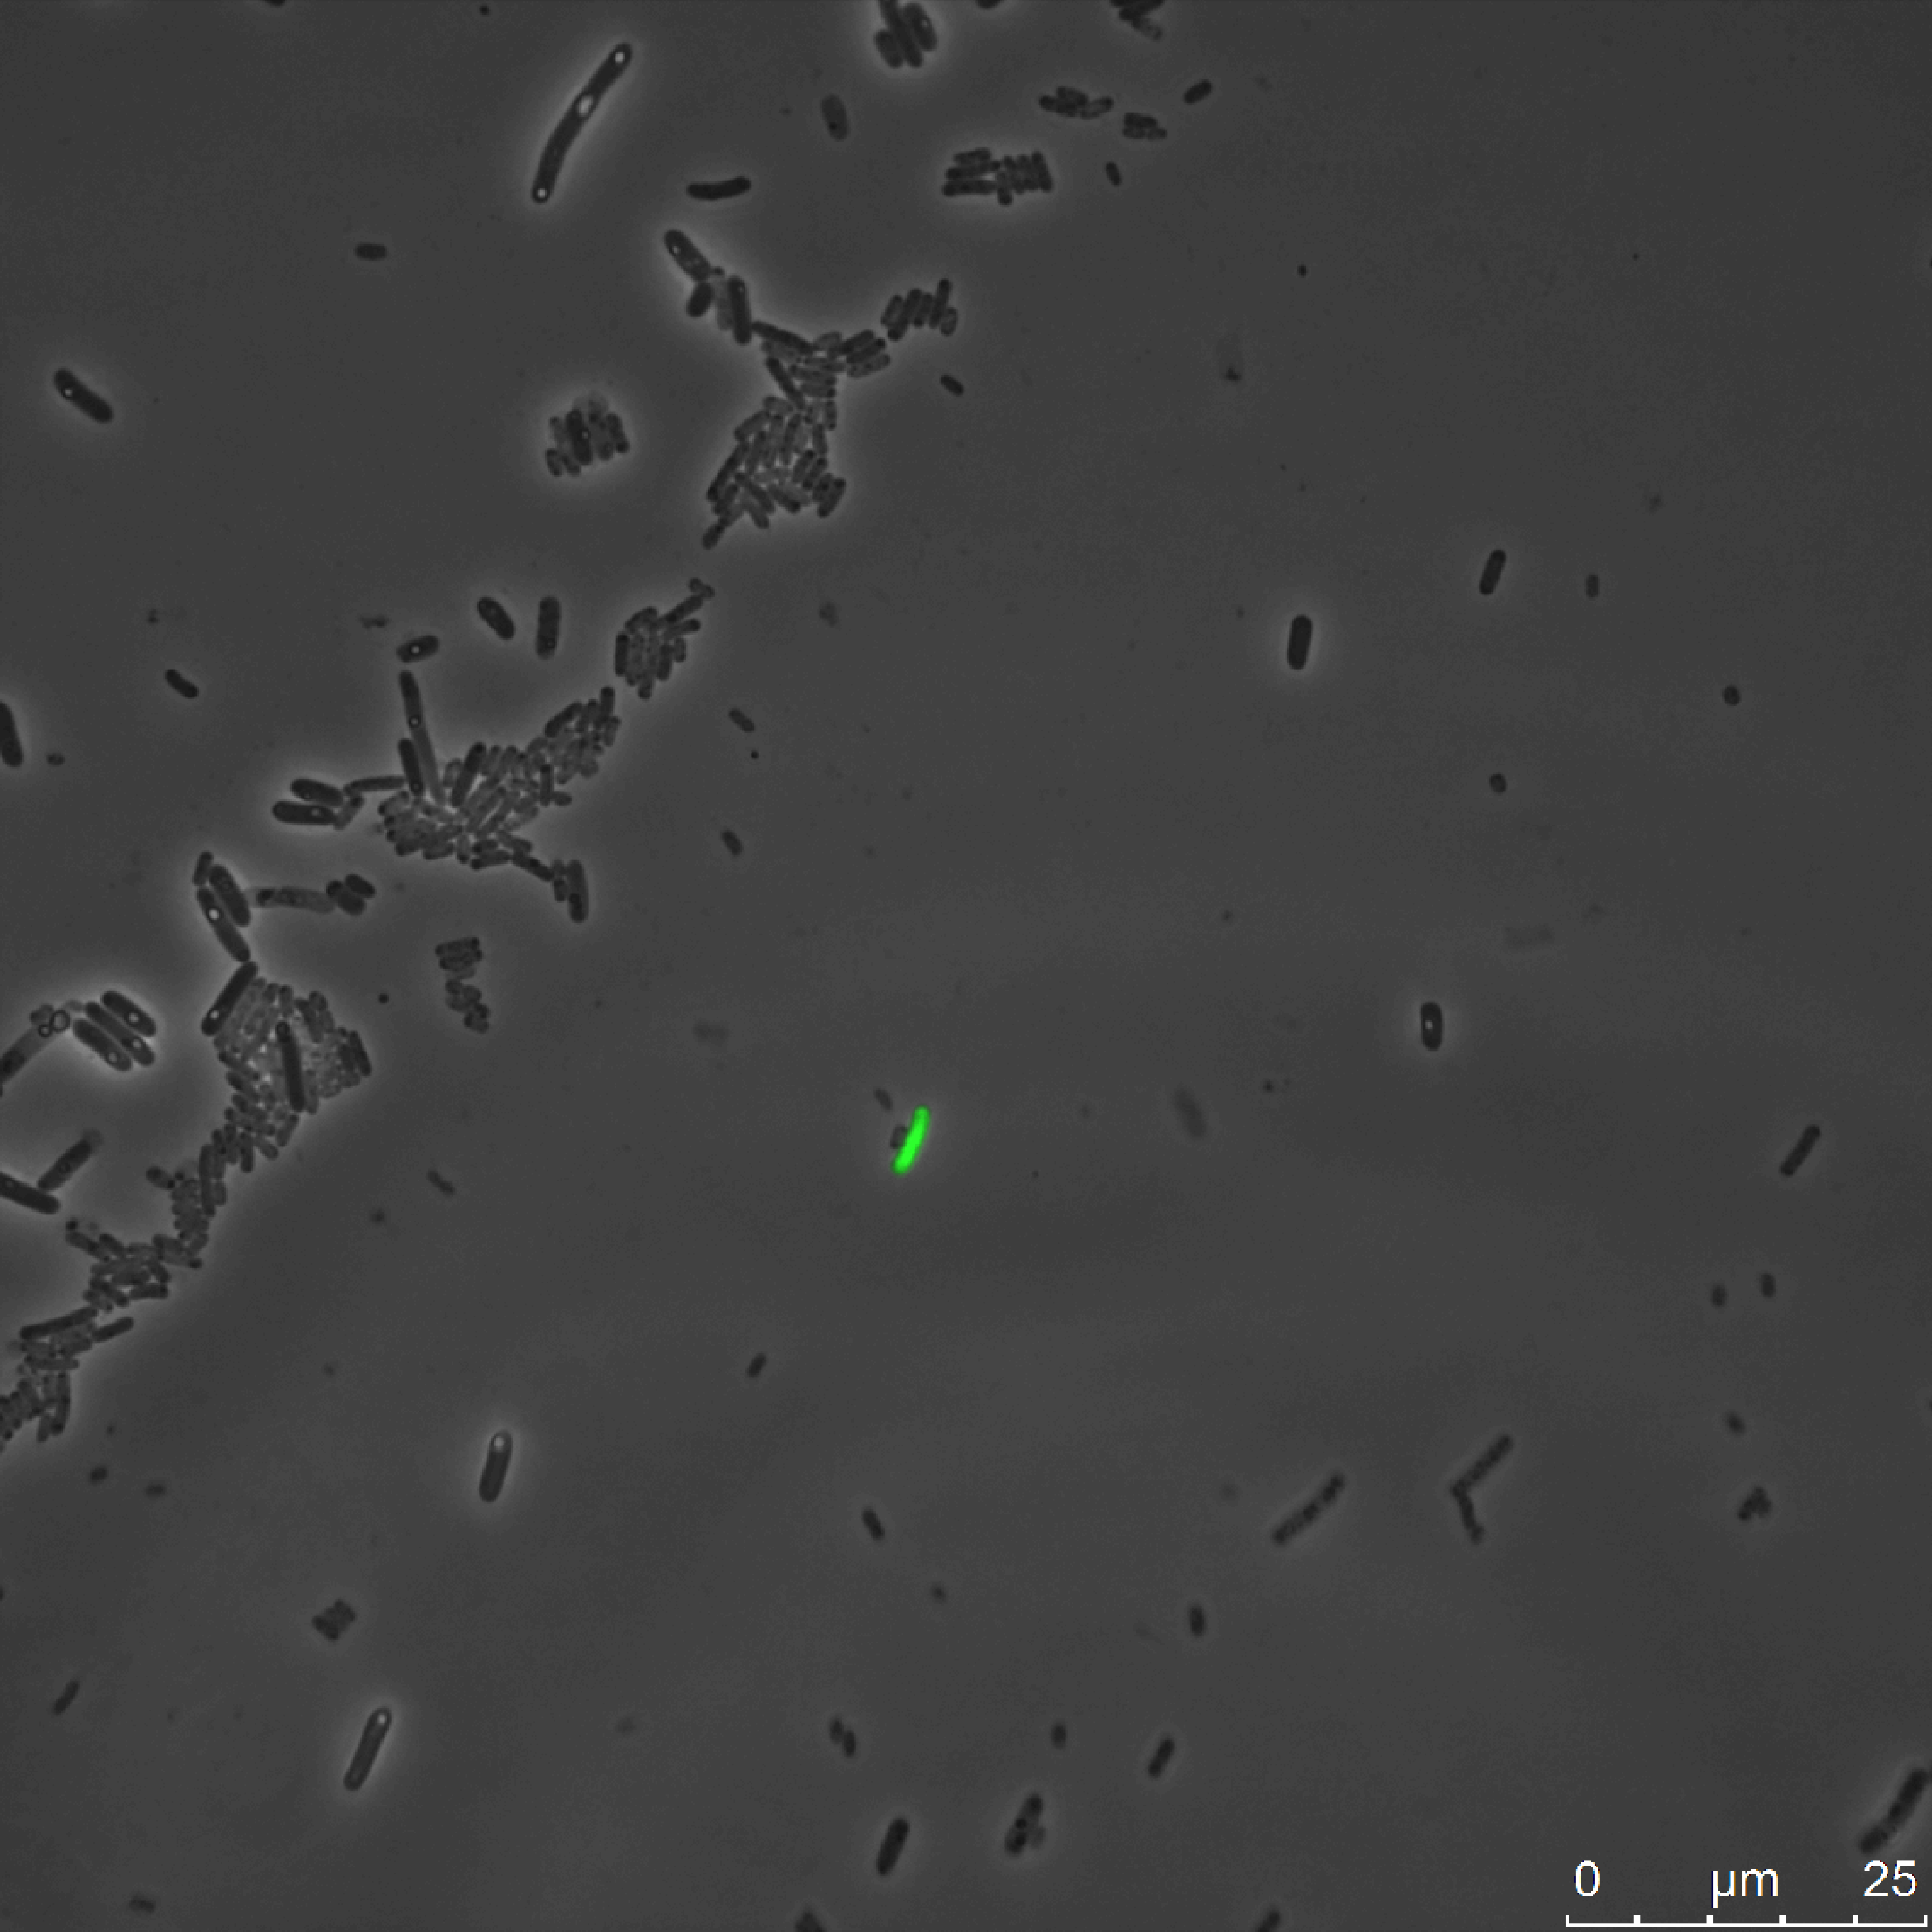
\includegraphics{TT01U4_72HR_2_GREEN.pdf} \\[-0.5ex]

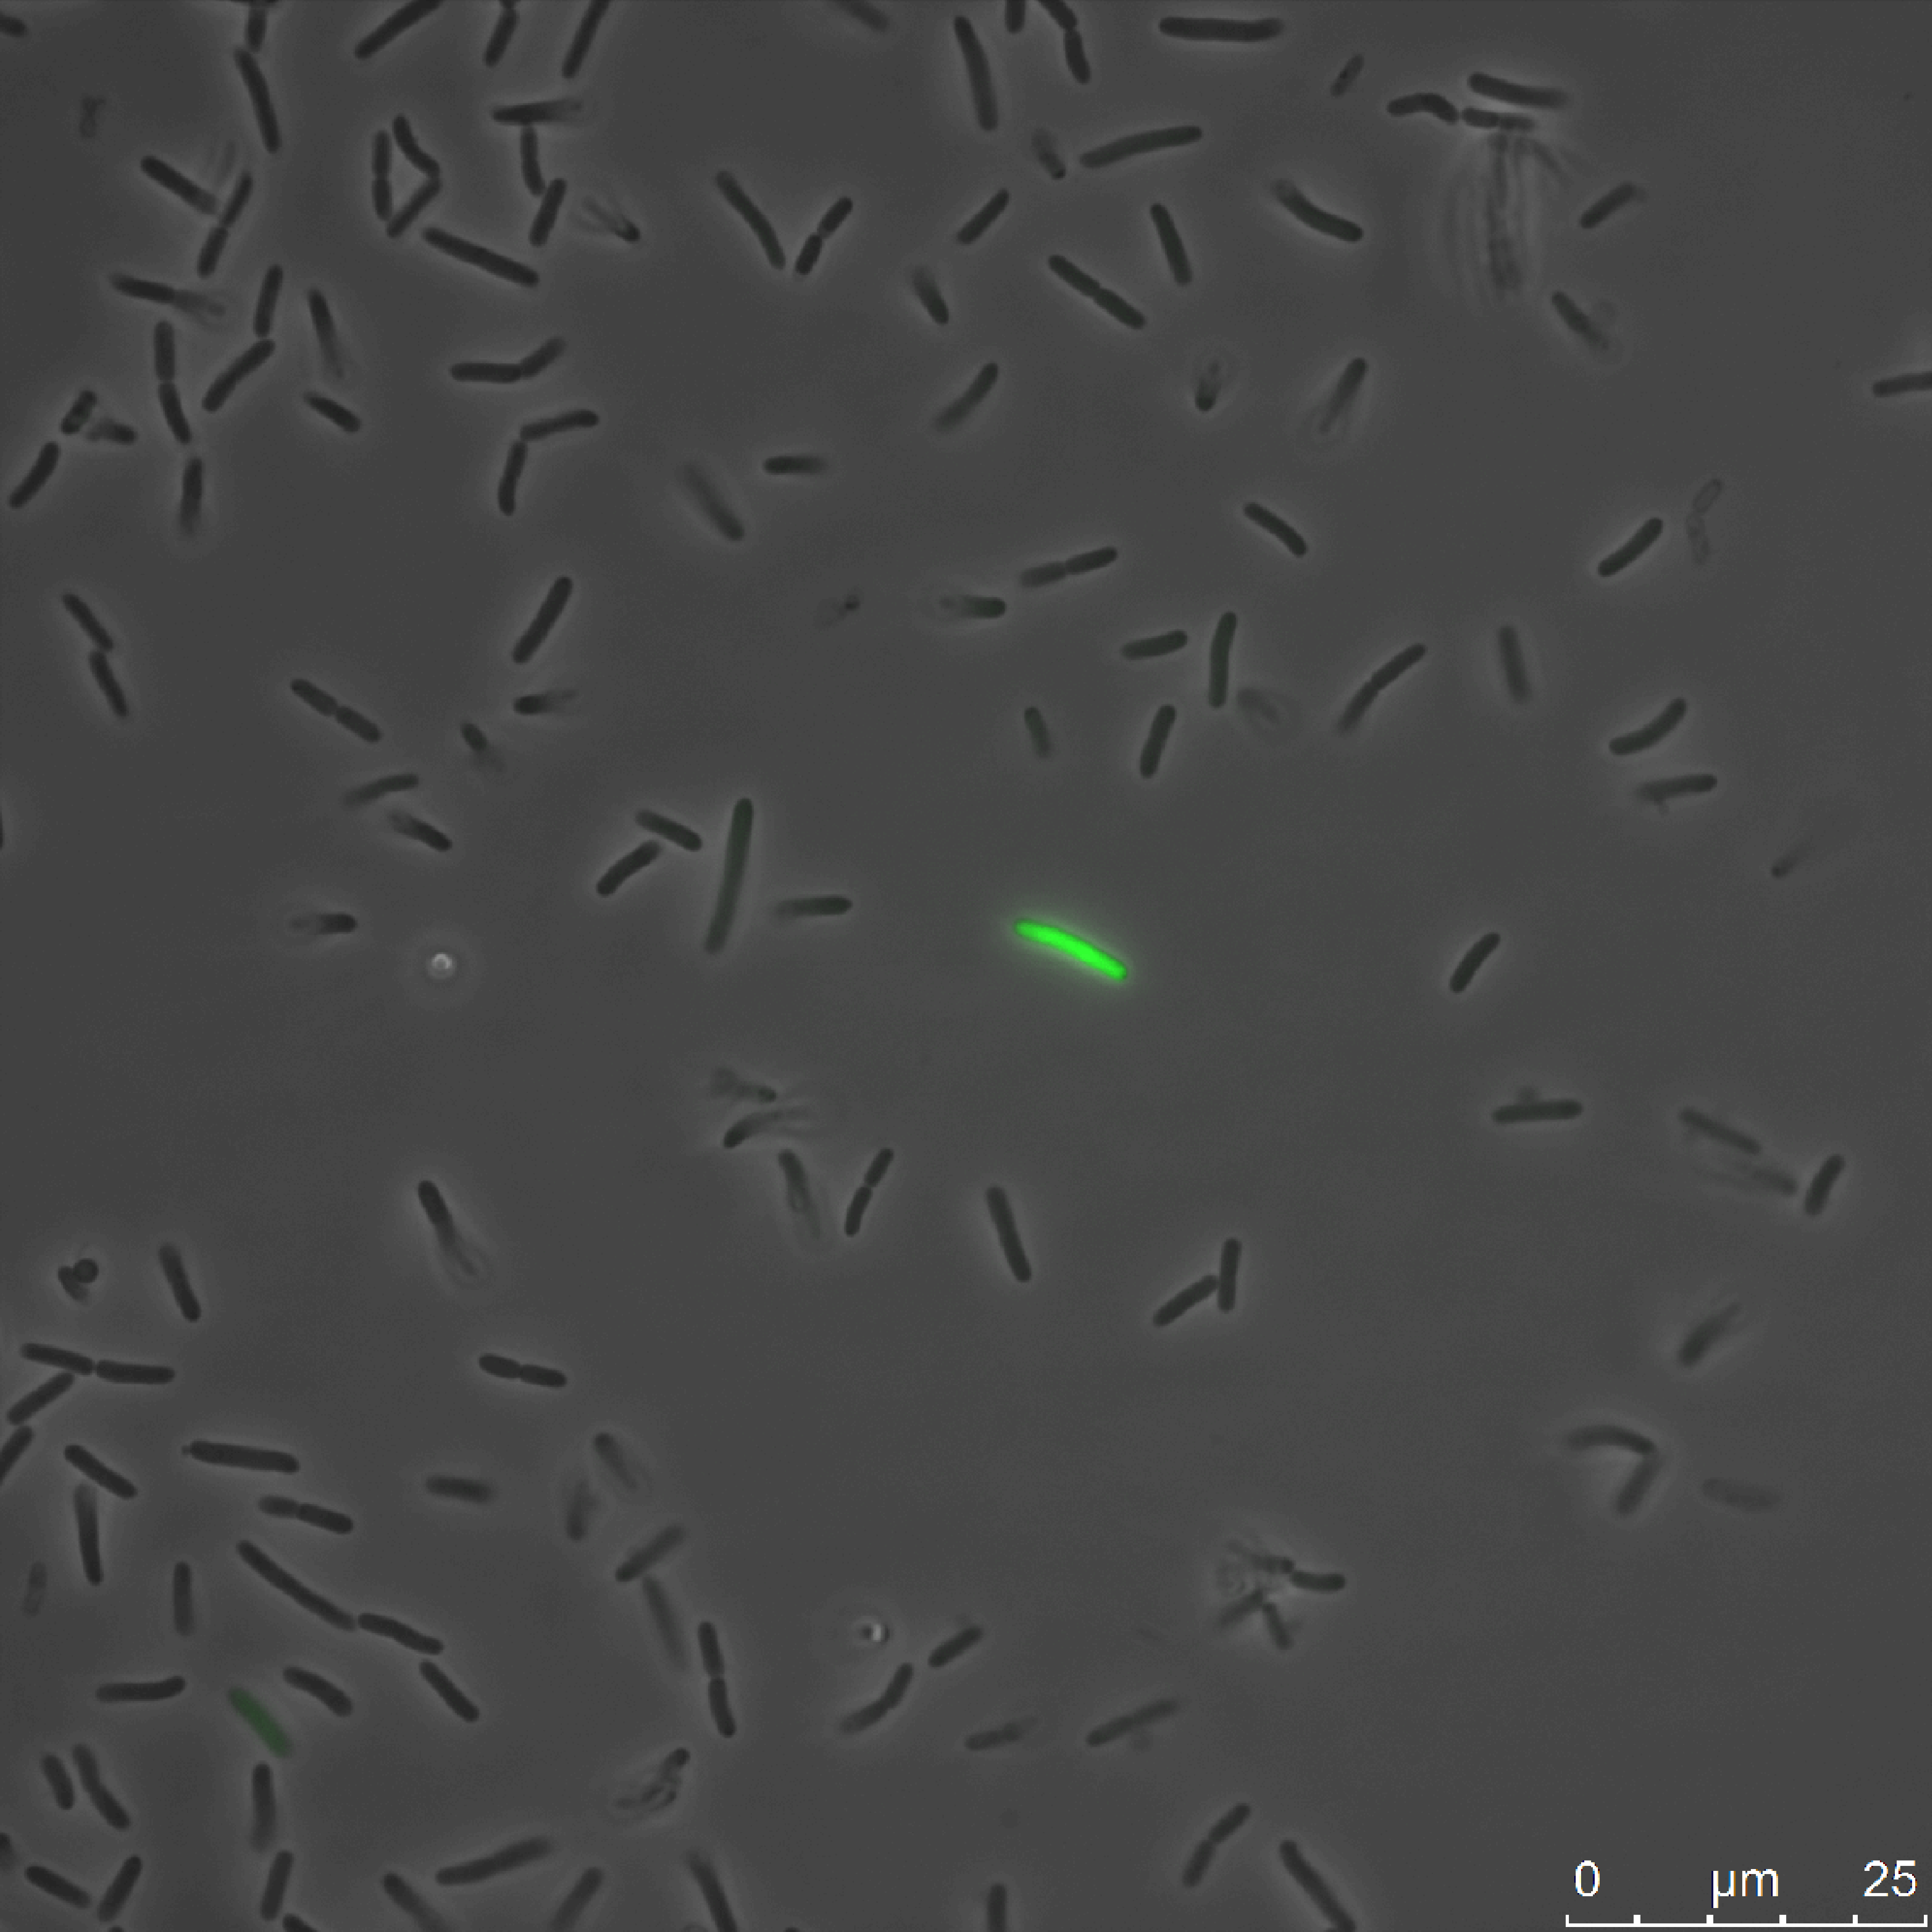
\includegraphics{TT01U4_5_GREEN.pdf} &%
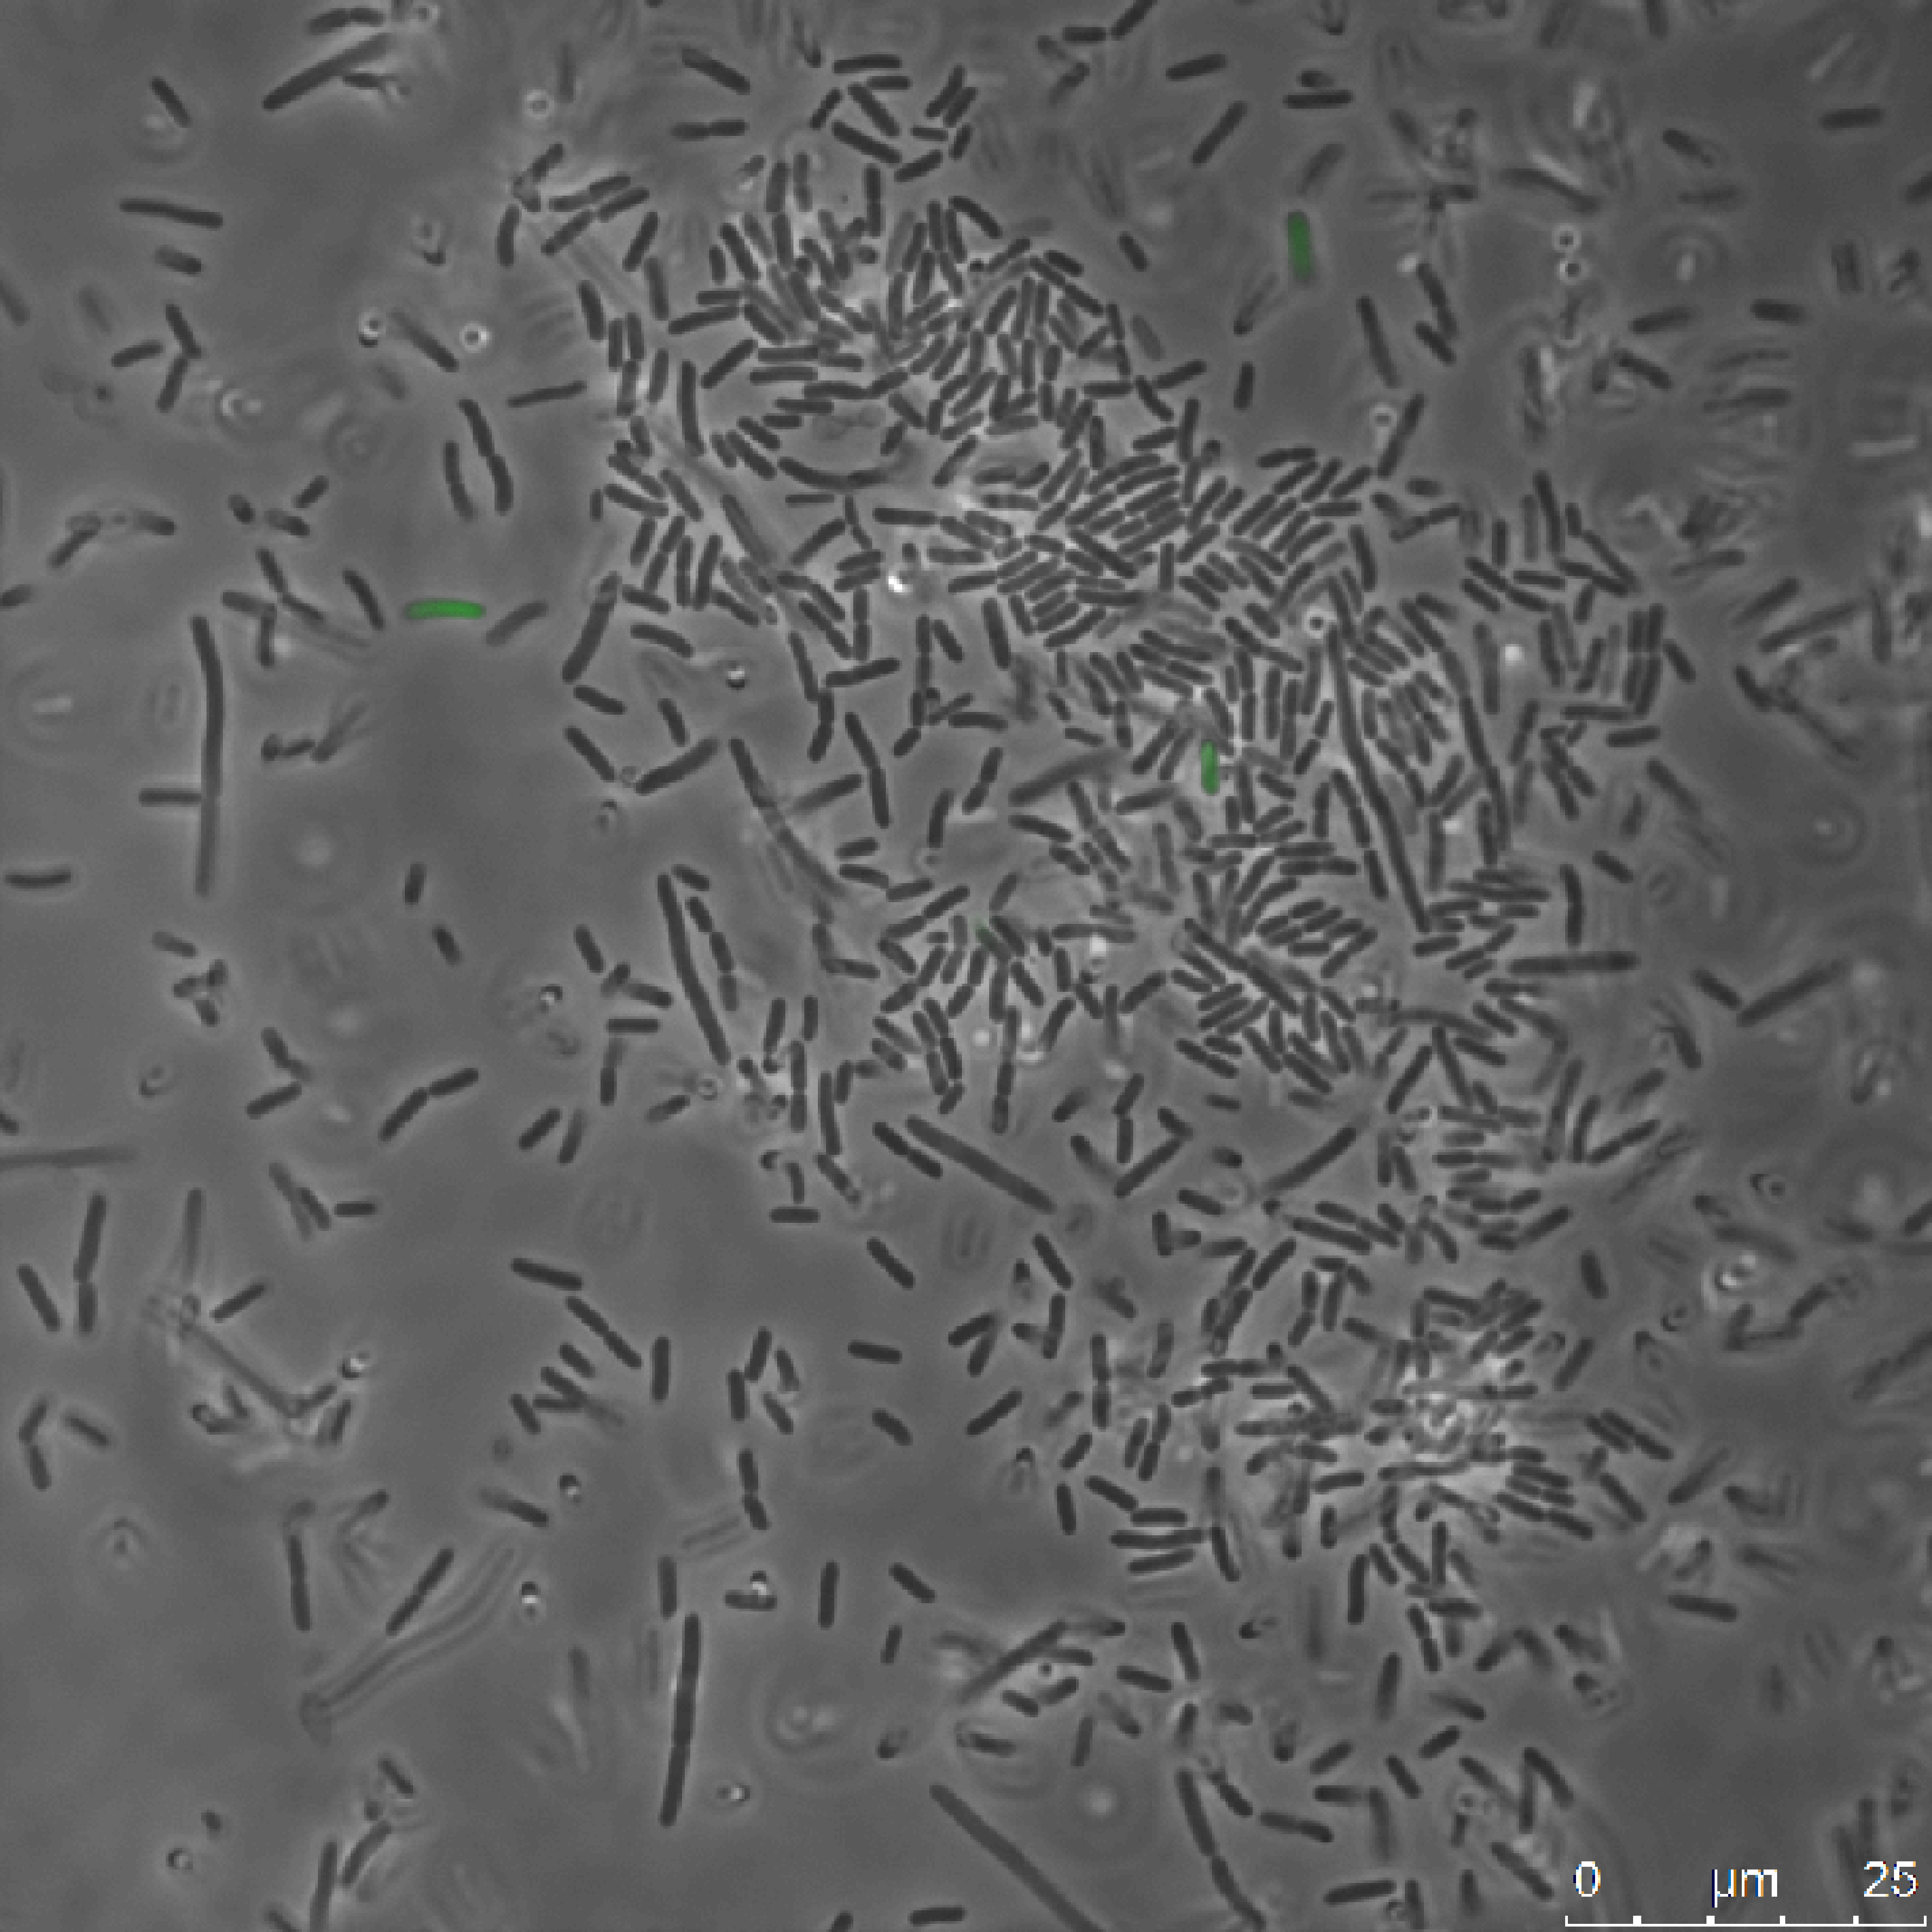
\includegraphics{TT01U4_5HR_3_GREEN.pdf} &%
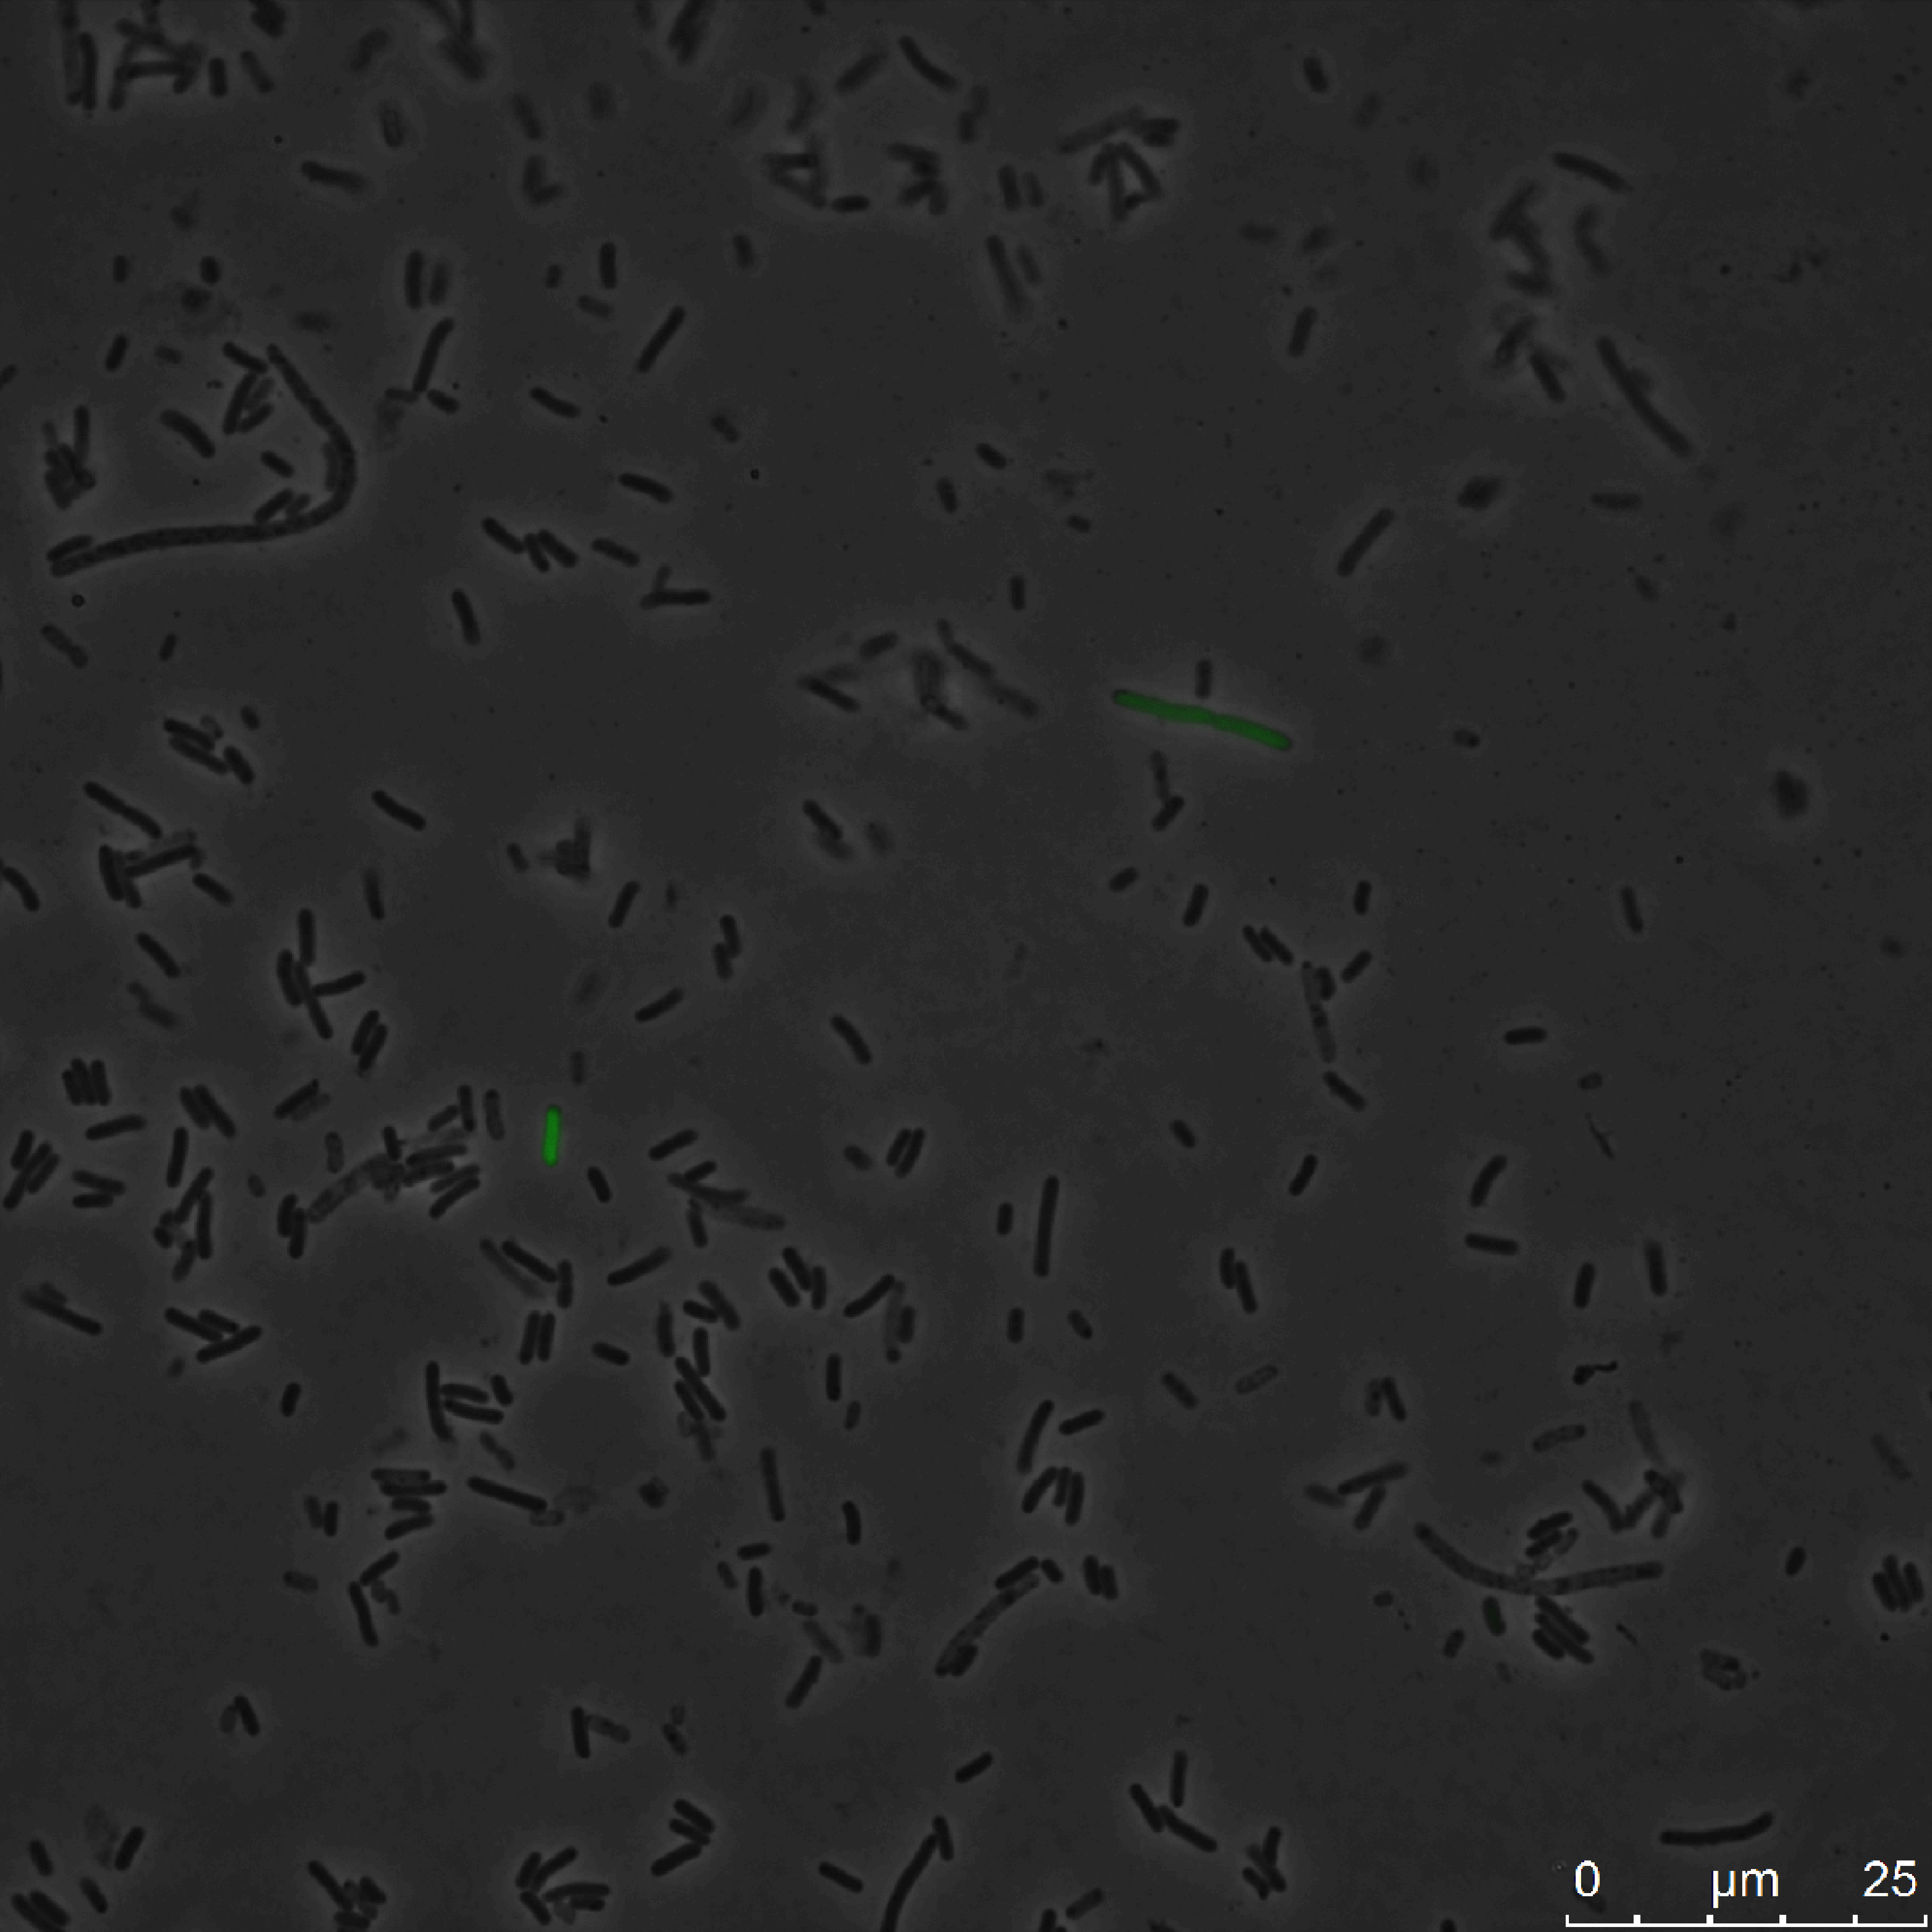
\includegraphics{TT01U4_24HR_3_GREEN.pdf} &%
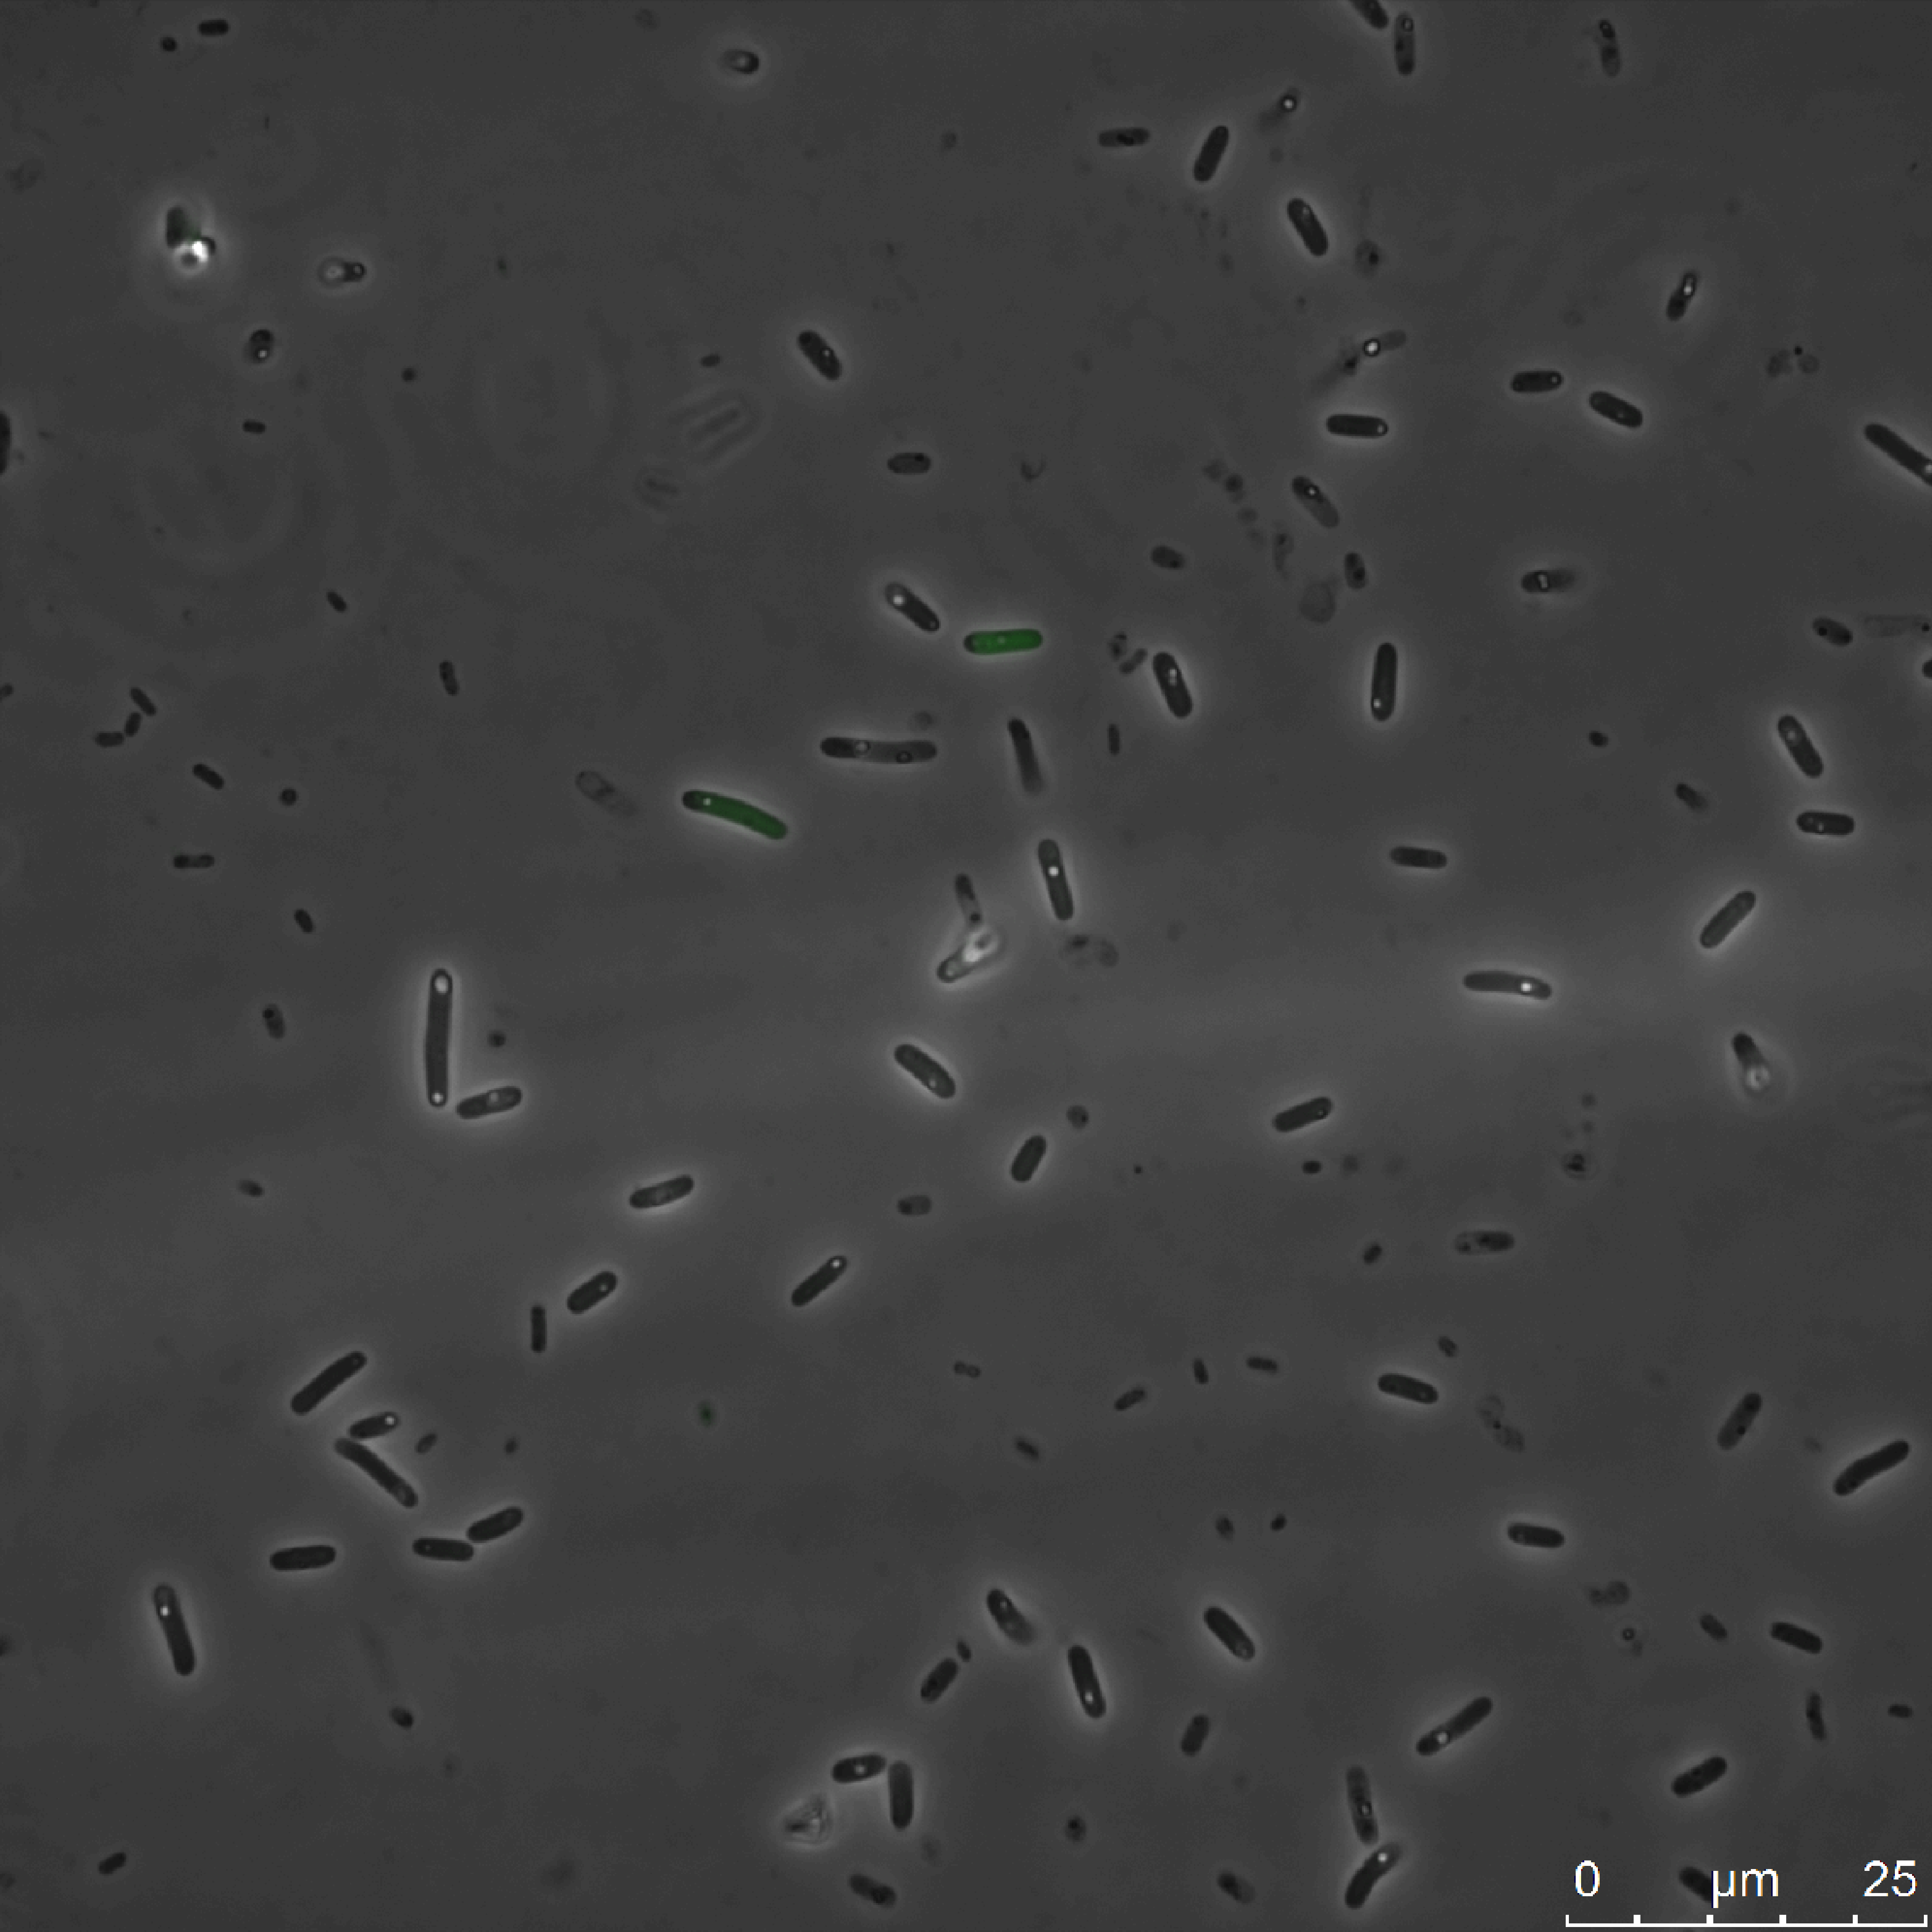
\includegraphics{TT01U4_72HR_3_GREEN.pdf} \\[-0.5ex]

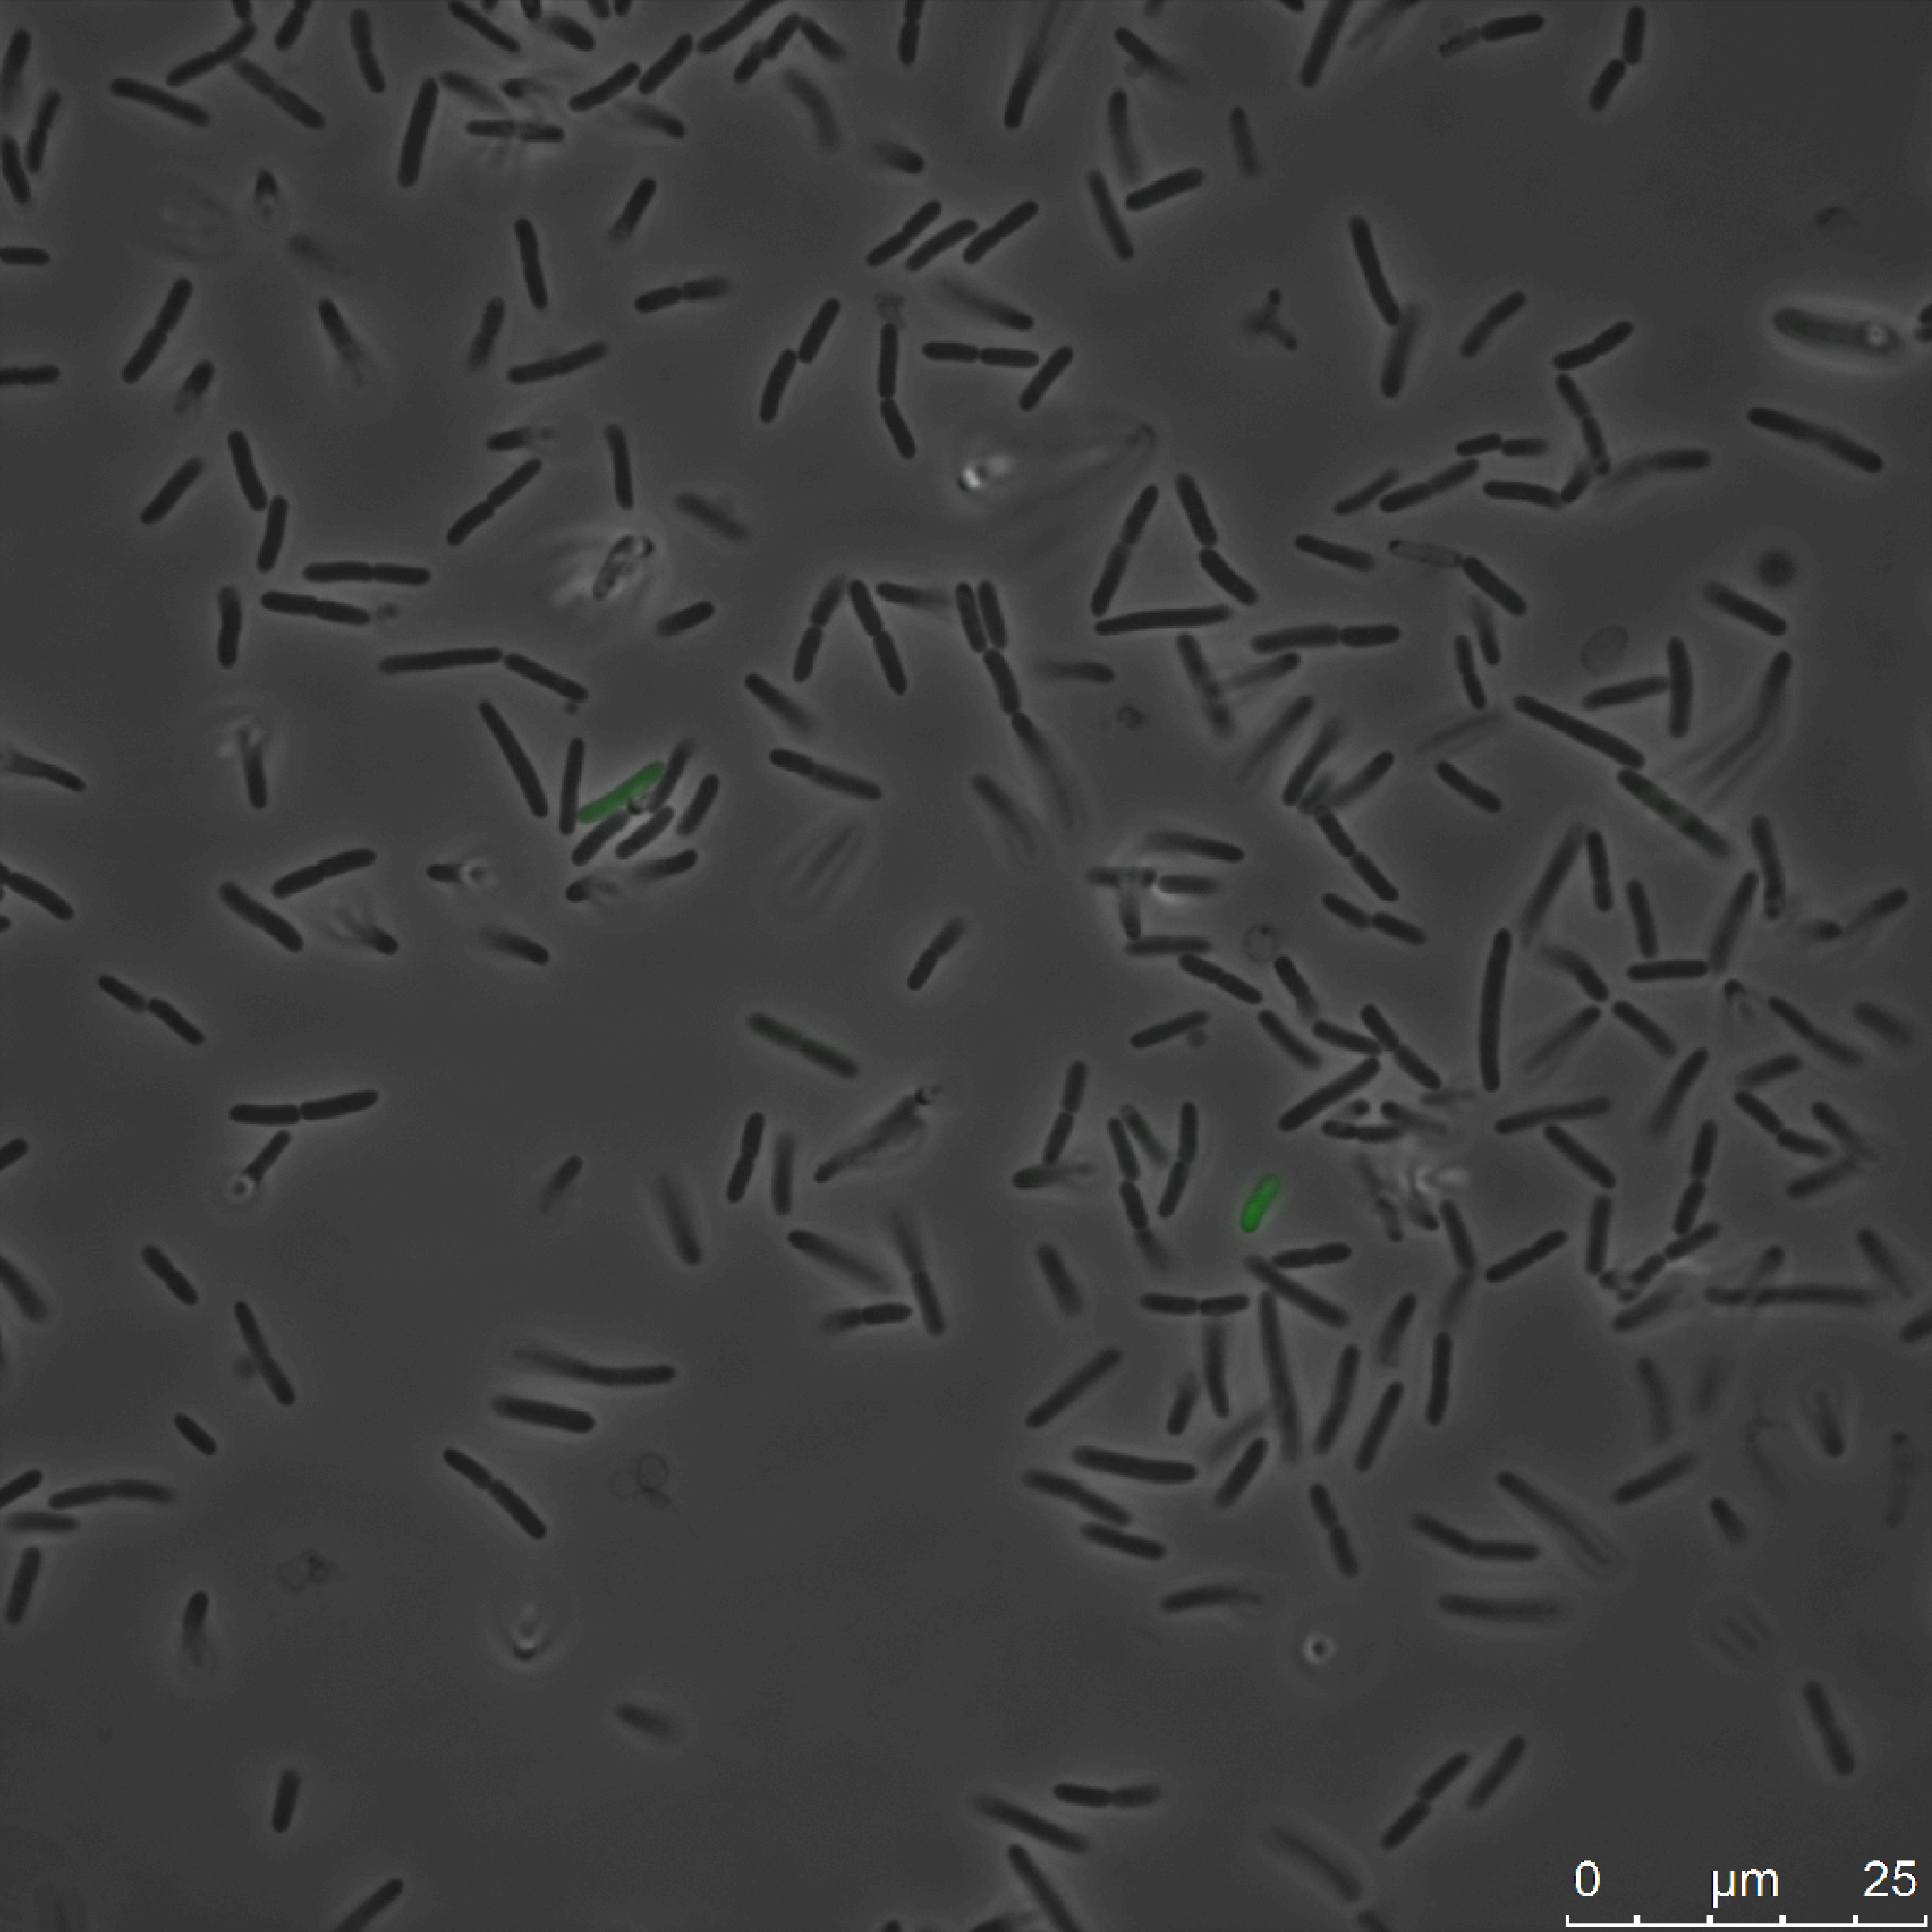
\includegraphics{TT01U4_6_GREEN.pdf} &%
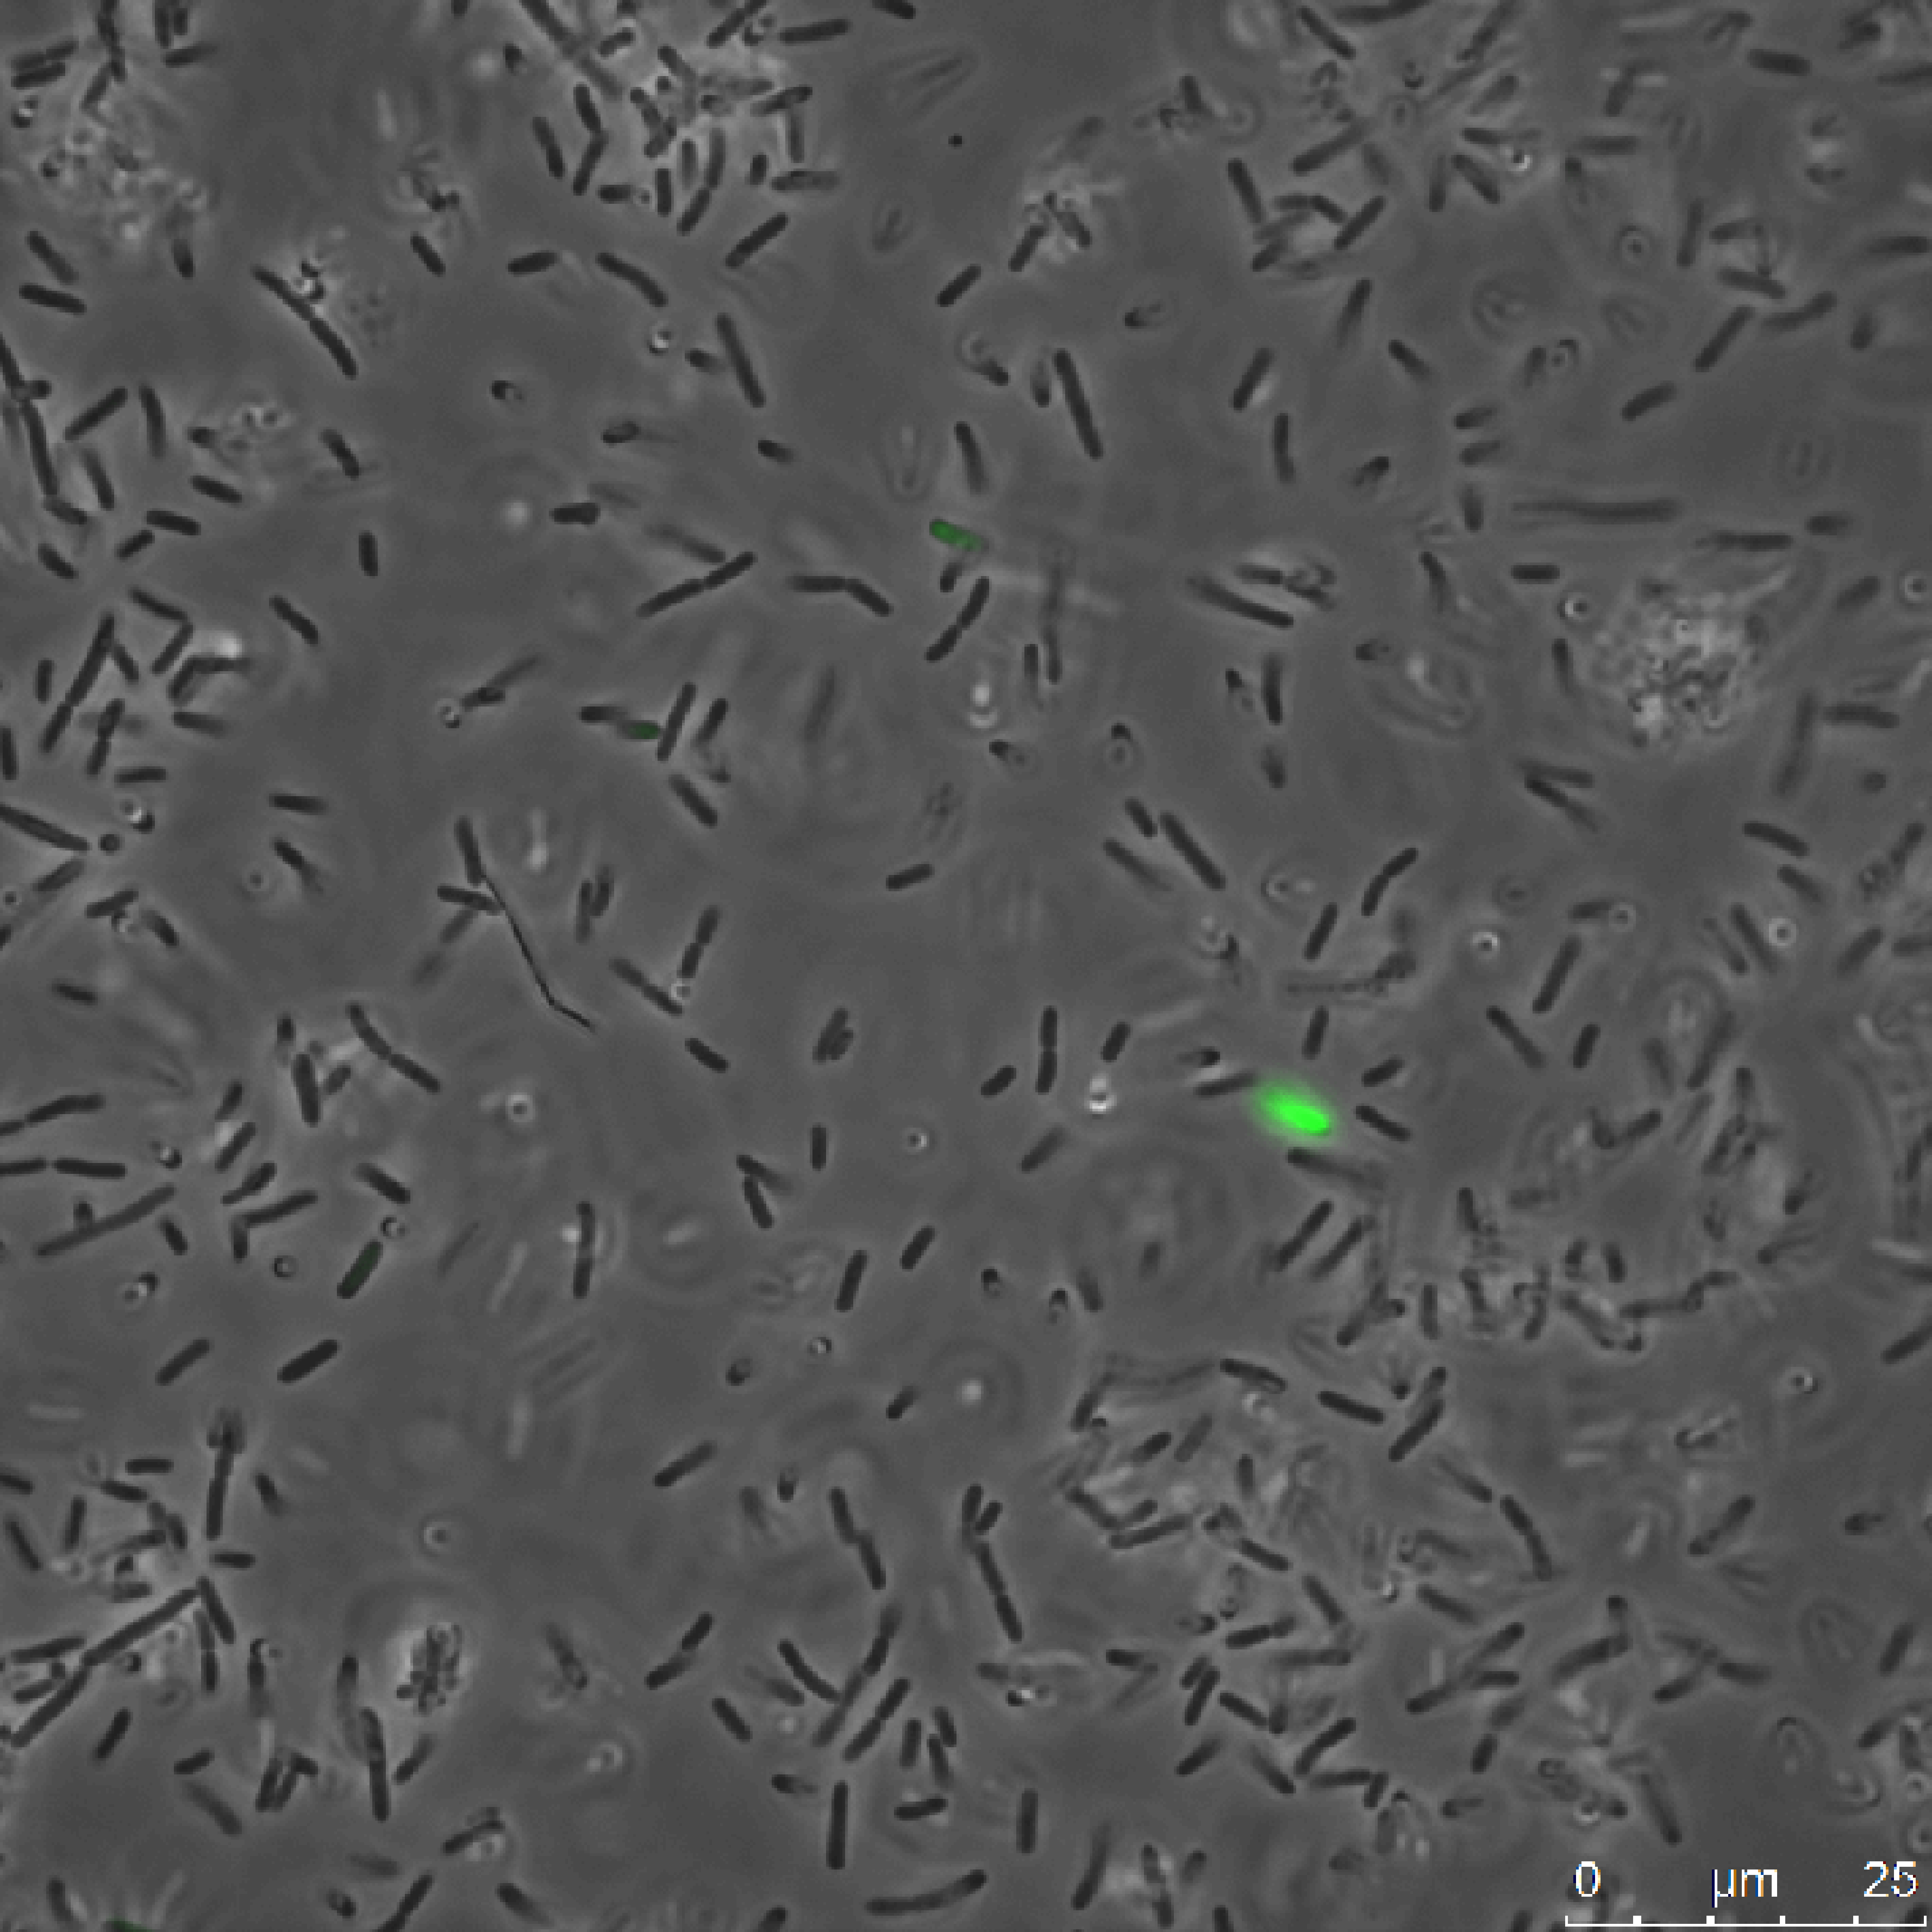
\includegraphics{TT01U4_5HR_4_GREEN.pdf} &%
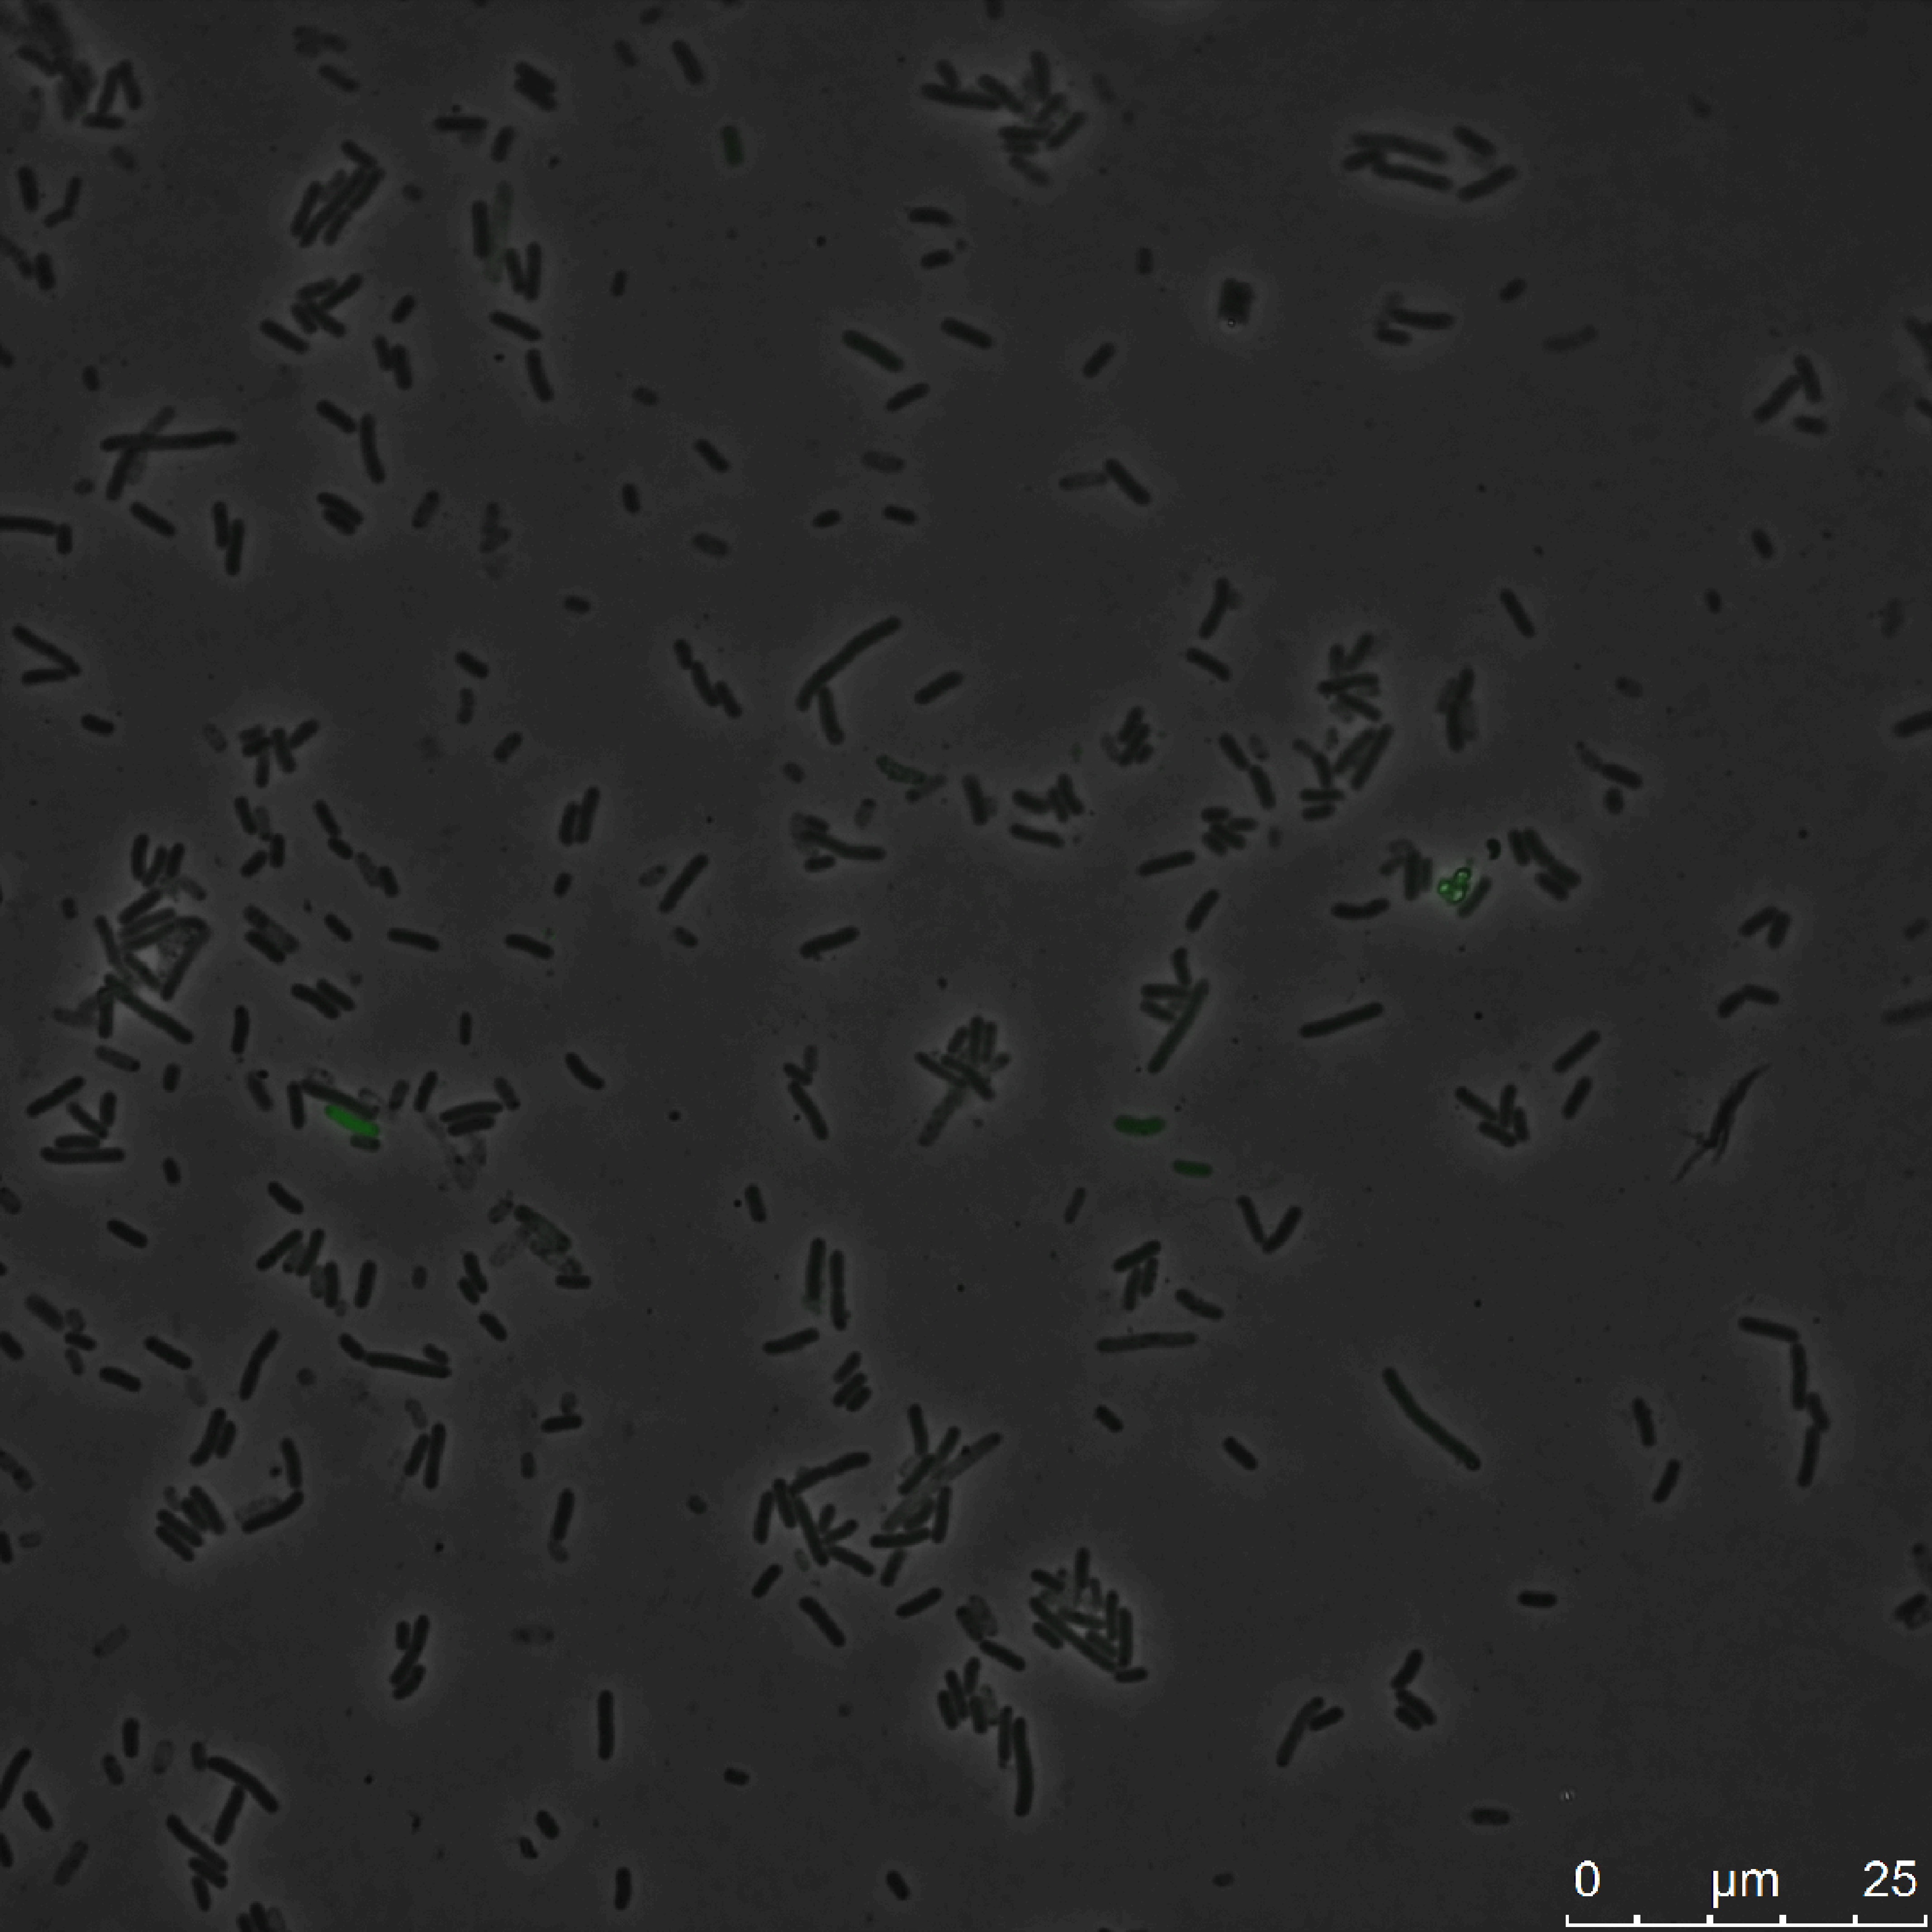
\includegraphics{TT01U4_24HR_4_GREEN.pdf} &%
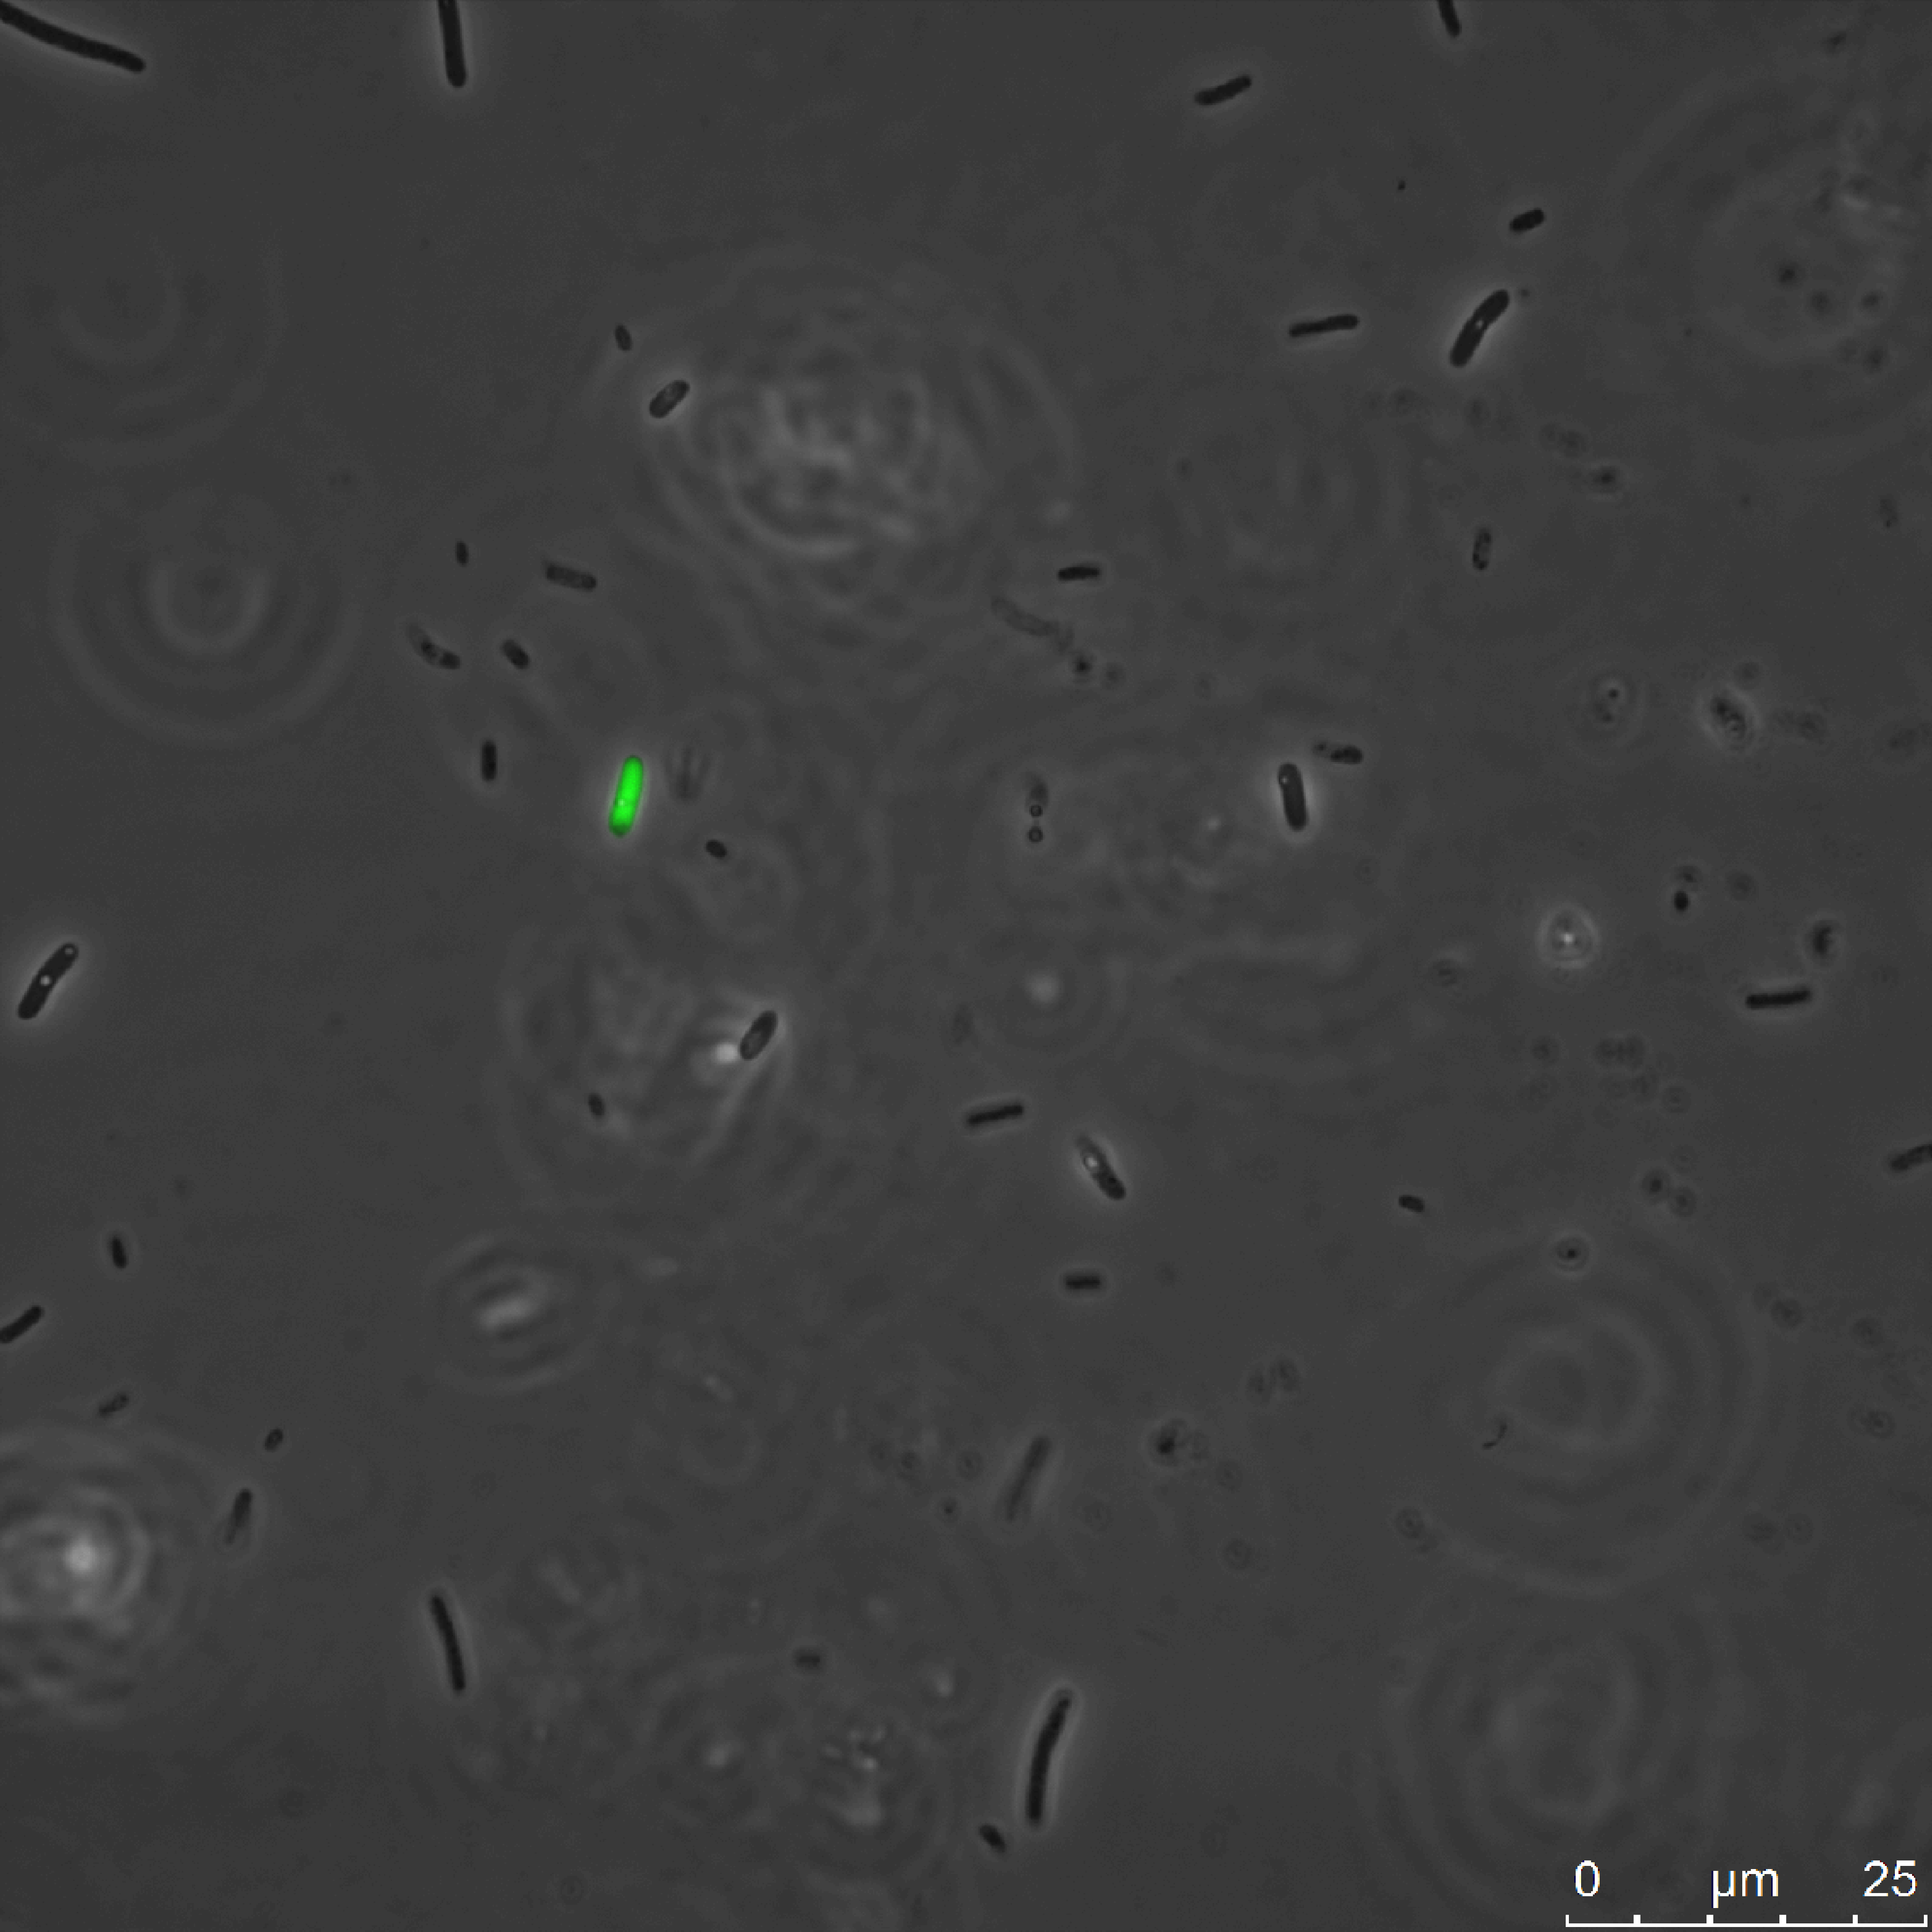
\includegraphics{TT01U4_72HR_4_GREEN.pdf} \\
 ++ & ++ & ++ & ++ \\[1ex]

\end{tabularx}

\label{RMTT01U4}
\captionsetup{singlelinecheck=off, justification=justified, font=footnotesize, aboveskip=20pt}
\caption[Reporter microscopy - TT01 Unit 4]{\textsc{\normalsize Reporter microscopy for the \emph{P. luminescens} TT01 ``Unit 4" promoter.}\vspace{0.1cm} \newline A representative selection of images for 4 time points, for the PVC ``Unit 4" promoter fusion. Quadruplicate images are displayed vertically as representative of the whole slide sample. Key to qualitative fluorescence indication: ``-" - no fluorescence, ``+" - low level fluorescence in isolated cells. ``++" - low level fluorescence in many cells or few brighter cells, ``+++" - intermediate to high fluorescence in almost all cells, or very bright isolated cells.}
\end{figure}
\endgroup

%%%%%%%%%%%%%%%%%%%%%%%%%%%%%%%%%%%%%%%%%%%%%%%%%%%%%%%%%%%%%%%%%%%%

\begingroup
\renewcommand{\arraystretch}{0.8}%
\setlength{\tabcolsep}{0.3pt}
\begin{figure}[p]
\setkeys{Gin}{width=\linewidth}
\Huge
\begin{tabularx}{\textwidth}{CCCC}
\multicolumn{4}{p{\linewidth}}{\large \centering \textbf{\emph{P. asymbiotica} PB68.1 (``THAI") PVC ``pnf"}} \\
\hiderowcolors
& & & \\[-1.5ex]
\Large 2 Hours &\Large 5 Hours &\Large 24 Hours &\Large 72 Hours \\[1ex]

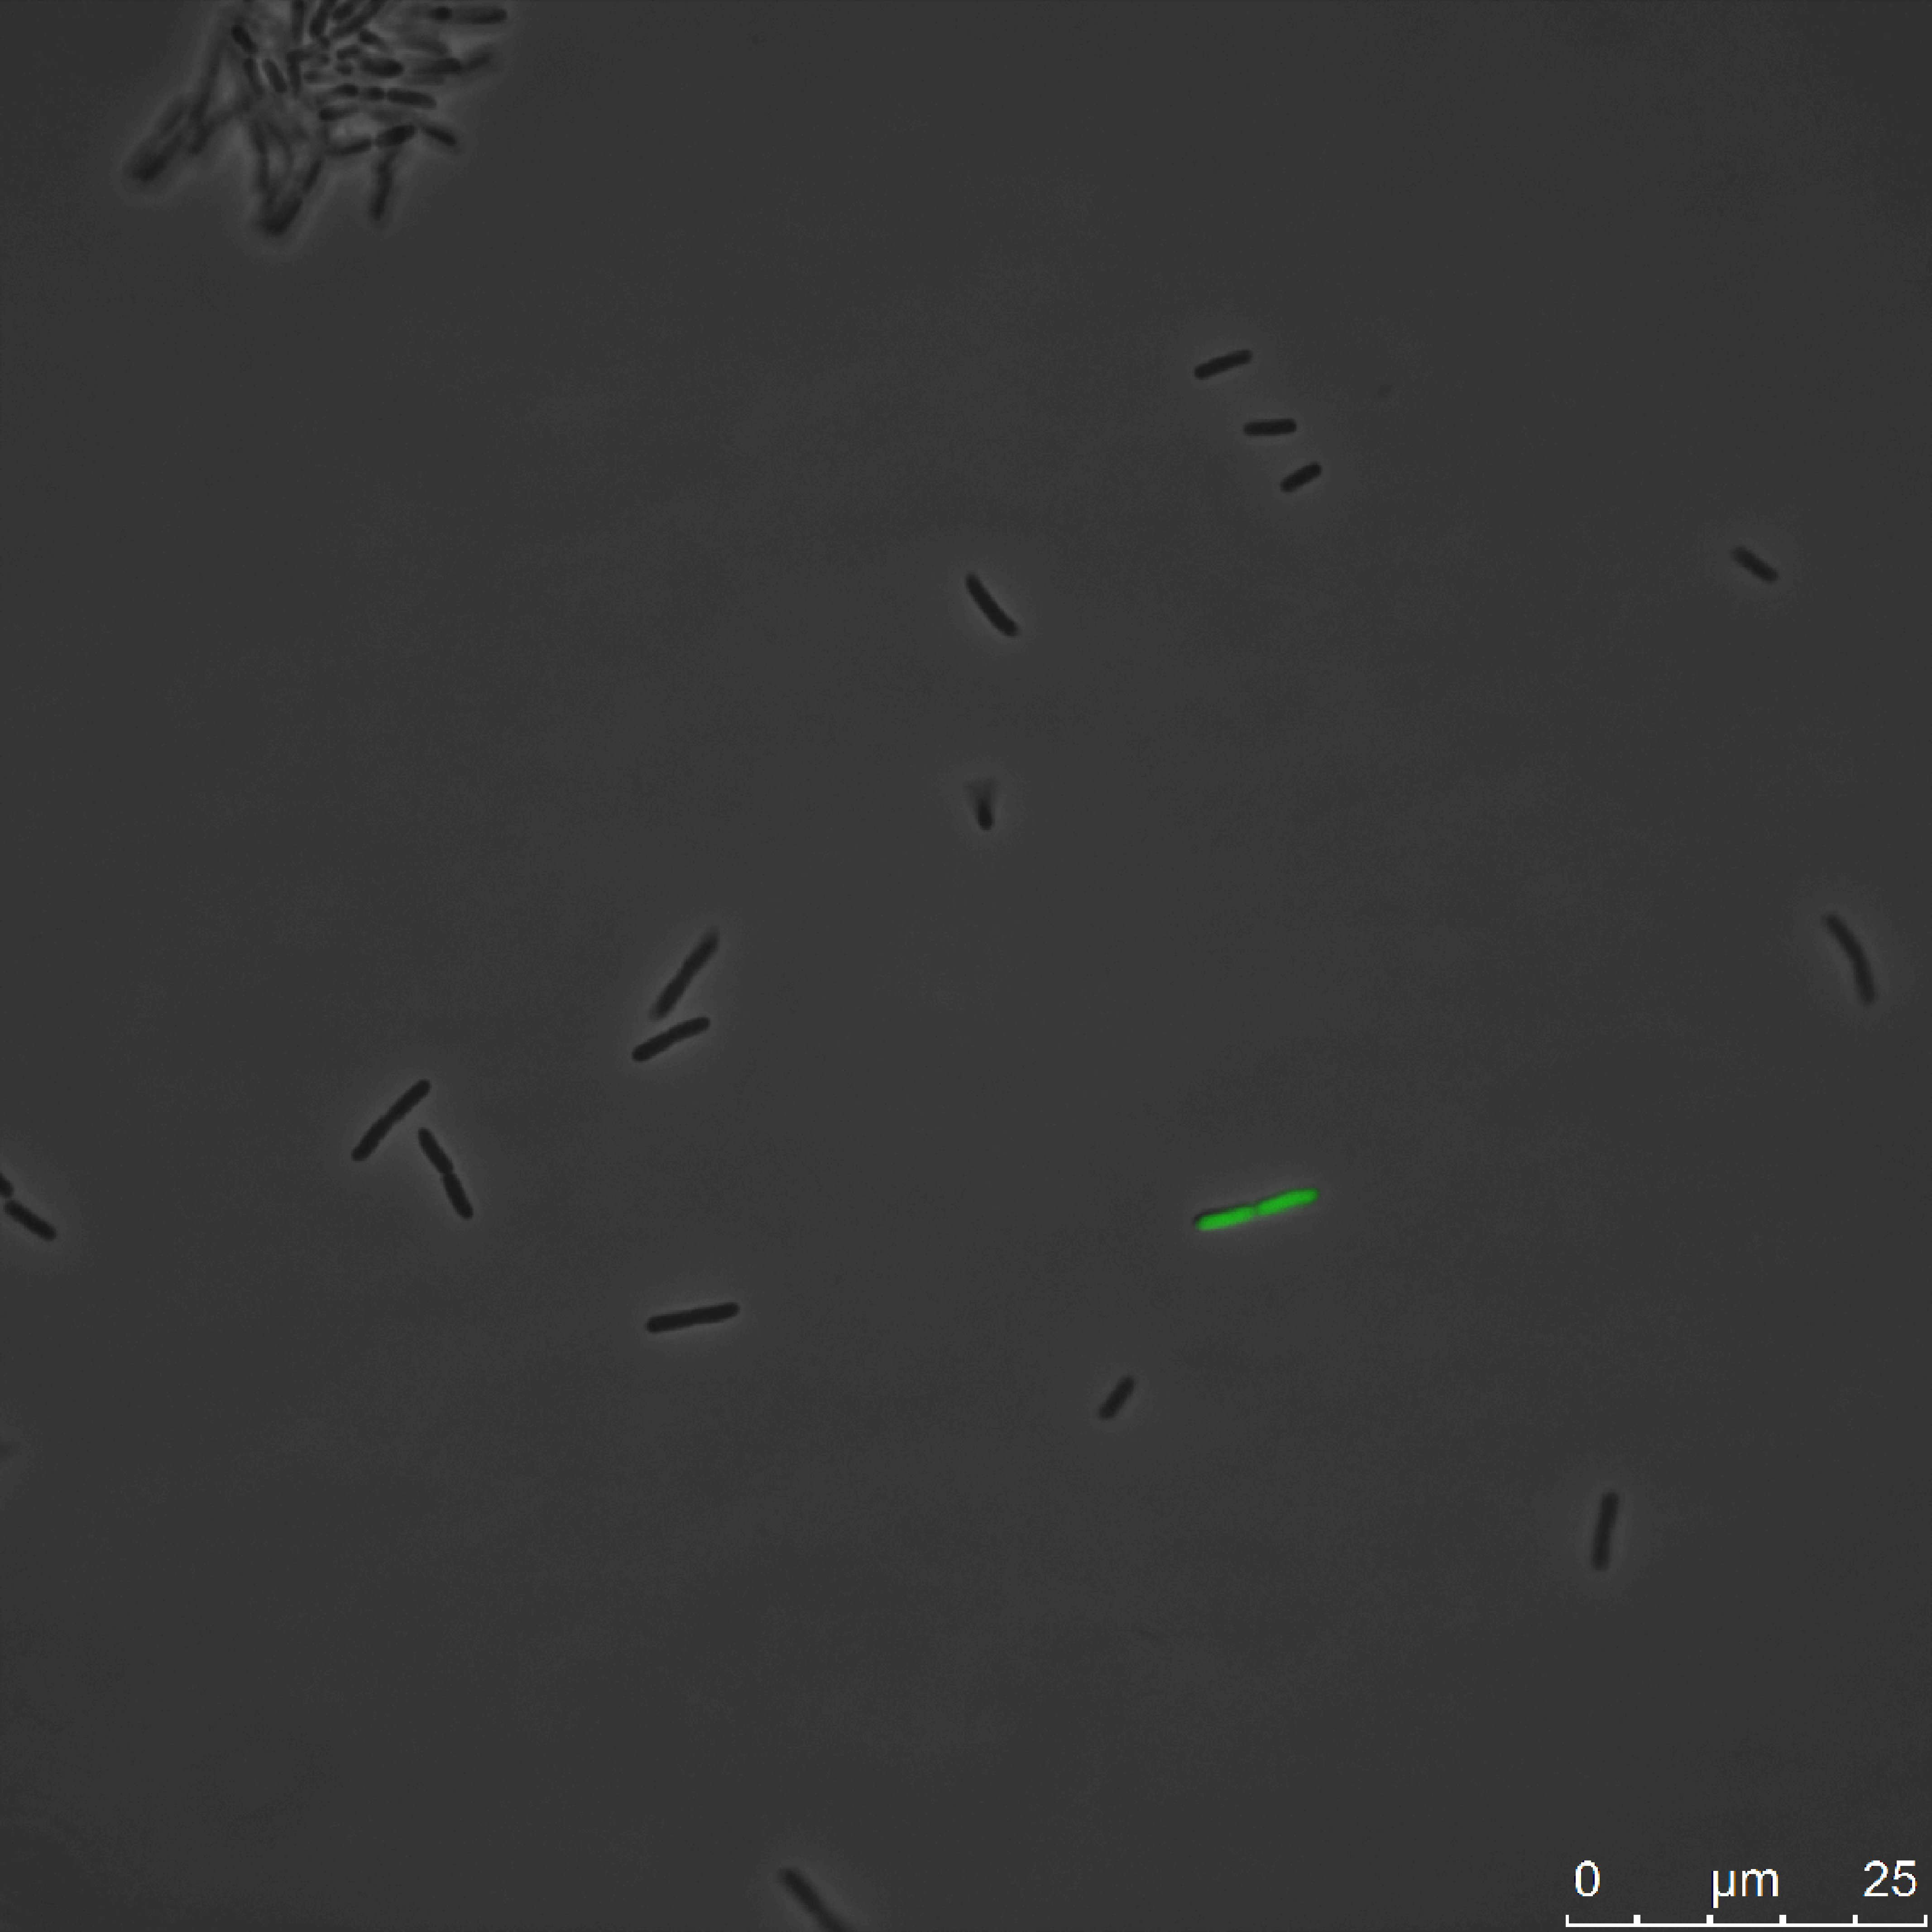
\includegraphics{THAIPNF_3_GREEN.pdf} &%
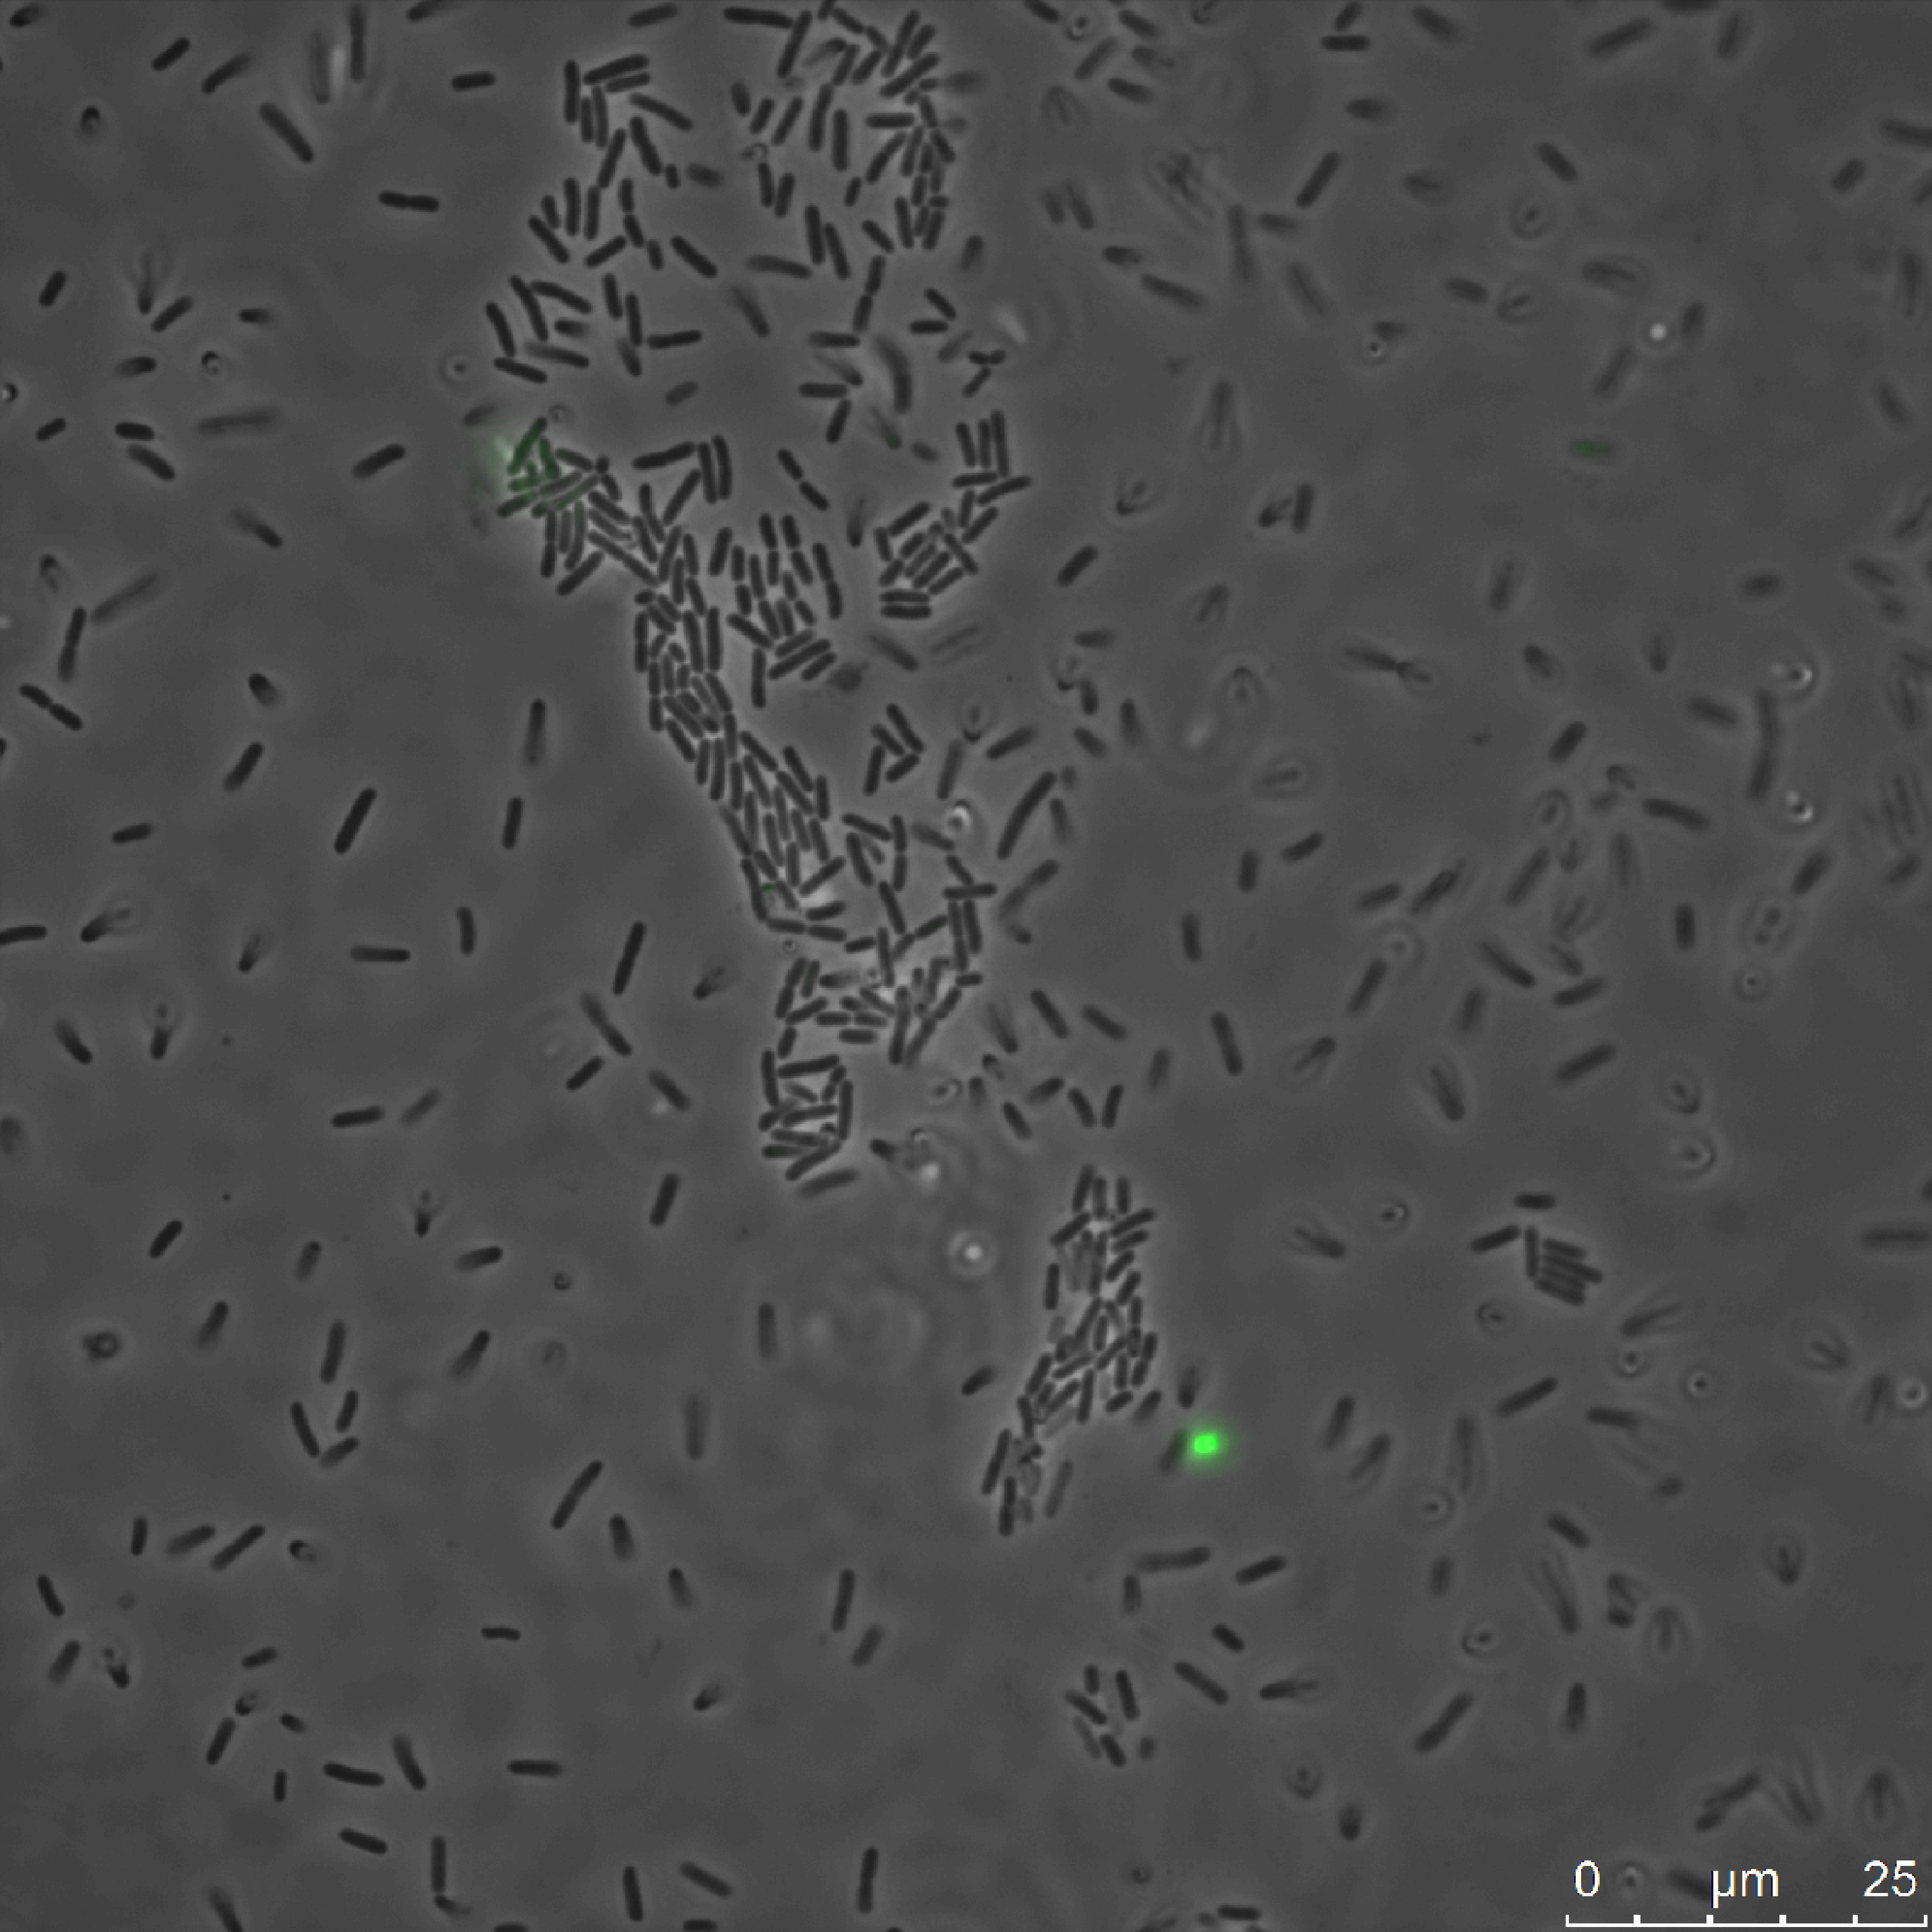
\includegraphics{THAIPNF_5HR_1_GREEN.pdf} &%
\includegraphics{THAIPNF_24HR_2_GREEN.pdf} &%
\includegraphics{THAIPNF_72HR_1_GREEN.pdf} \\[-0.5ex]

\includegraphics{THAIPNF_4_GREEN.pdf} &%
\includegraphics{THAIPNF_5HR_2_GREEN.pdf} &%
\includegraphics{THAIPNF_24HR_4_GREEN.pdf} &%
\includegraphics{THAIPNF_72HR_2_GREEN.pdf} \\[-0.5ex]

\includegraphics{THAIPNF_5_GREEN.pdf} &%
\includegraphics{THAIPNF_5HR_3_GREEN.pdf} &%
\includegraphics{THAIPNF_24HR_5_GREEN.pdf} &%
\includegraphics{THAIPNF_72HR_3_GREEN.pdf} \\[-0.5ex]

\includegraphics{THAIPNF_6_GREEN.pdf} &%
\includegraphics{THAIPNF_5HR_4_GREEN.pdf} &%
\includegraphics{THAIPNF_24HR_7_GREEN.pdf} &%
\includegraphics{THAIPNF_72HR_4_GREEN.pdf} \\
 +++ & +++ & +++ & +++ \\[1ex]

\end{tabularx}

\label{RMTHAIPNF}
\captionsetup{singlelinecheck=off, justification=justified, font=footnotesize, aboveskip=20pt}
\caption[Reporter microscopy - PB68.1 pnf]{\textsc{\normalsize Reporter microscopy for the \emph{P. asymbiotica} PB68.1 ``pnf" promoter.}\vspace{0.1cm} \newline A representative selection of images for 4 time points, for the PVC ``pnf" promoter fusion. Quadruplicate images are displayed vertically as representative of the whole slide sample. Key to qualitative fluorescence indication: ``-" - no fluorescence, ``+" - low level fluorescence in isolated cells. ``++" - low level fluorescence in many cells or few brighter cells, ``+++" - intermediate to high fluorescence in almost all cells, or very bright isolated cells.}
\end{figure}
\endgroup

%%%%%%%%%%%%%%%%%%%%%%%%%%%%%%%%%%%%%%%%%%%%%%%%%%%%%%%%%%%%%%%%%%%%

\begingroup
\renewcommand{\arraystretch}{0.8}%
\setlength{\tabcolsep}{0.3pt}
\begin{figure}[p]
\setkeys{Gin}{width=\linewidth}
\Huge
\begin{tabularx}{\textwidth}{CCCC}
\multicolumn{4}{p{\linewidth}}{\large \centering \textbf{\emph{P. luminescens} TT01 PVC ``LopT"}} \\
\hiderowcolors
& & & \\[-1.5ex]
\Large 2 Hours &\Large 5 Hours &\Large 24 Hours &\Large 72 Hours \\[1ex]

\includegraphics{TT01LOPT_1_LOWGREEN.pdf} &%
\includegraphics{TT01LOPT_5HR_1_LOWGREEN.pdf} &%
\includegraphics{TT01LOPT_24HR_1_GREEN.pdf} &%
\includegraphics{TT01LOPT_72HR_1_GREEN.pdf} \\[-0.5ex]

\includegraphics{TT01LOPT_2_NOGREEN.pdf} &%
\includegraphics{TT01LOPT_5HR_2_LOWGREEN.pdf} &%
\includegraphics{TT01LOPT_24HR_2_GREEN.pdf} &%
\includegraphics{TT01LOPT_72HR_2_GREEN.pdf} \\[-0.5ex]

\includegraphics{TT01LOPT_3_LOWGREEN.pdf} &%
\includegraphics{TT01LOPT_5HR_3_LOWGREEN.pdf} &%
\includegraphics{TT01LOPT_24HR_3_GREEN.pdf} &%
\includegraphics{TT01LOPT_72HR_3_GREEN.pdf} \\[-0.5ex]

\includegraphics{TT01LOPT_4_LOWGREEN} &%
\includegraphics{TT01LOPT_5HR_4_LOWGREEN.pdf} &%
\includegraphics{TT01LOPT_24HR_7_GREEN.pdf} &%
\includegraphics{TT01LOPT_72HR_6_GREEN.pdf} \\
 + & + & +++ & ++ \\[1ex]

\end{tabularx}

\label{RMTT01LOPT}
\captionsetup{singlelinecheck=off, justification=justified, font=footnotesize, aboveskip=20pt}
\caption[Reporter microscopy - TT01 LopT]{\textsc{\normalsize Reporter microscopy for the \emph{P. luminescens} TT01 ``LopT" promoter.}\vspace{0.1cm} \newline A representative selection of images for 4 time points, for the PVC ``LopT" promoter fusion. Quadruplicate images are displayed vertically as representative of the whole slide sample. Key to qualitative fluorescence indication: ``-" - no fluorescence, ``+" - low level fluorescence in isolated cells. ``++" - low level fluorescence in many cells or few brighter cells, ``+++" - intermediate to high fluorescence in almost all cells, or very bright isolated cells.}
\end{figure}
\endgroup

%%%%%%%%%%%%%%%%%%%%%%%%%%%%%%%%%%%%%%%%%%%%%%%%%%%%%%%%%%%%%%%%%%%%


\begingroup
\renewcommand{\arraystretch}{0.8}%
\setlength{\tabcolsep}{0.3pt}
\begin{figure}[p]
\setkeys{Gin}{width=\linewidth}
\Huge
\begin{tabularx}{\textwidth}{CCCC}
\multicolumn{4}{p{\linewidth}}{\large \centering \textbf{\emph{P. asymbiotica} PB68.1 (``THAI") PVC ``LopT"}} \\
\hiderowcolors
& & & \\[-1.5ex]
\Large 2 Hours &\Large 5 Hours &\Large 24 Hours &\Large 72 Hours \\[1ex]

\includegraphics{THAILOPT_1_NOGREEN.pdf} &%
\includegraphics{THAILOPT_5HR_1_NOGREEN.pdf} &%
\includegraphics{THAILOPT_24HR_1_NOGREEN.pdf} &%
\includegraphics{THAILOPT_72HR_1_NOGREEN.pdf} \\[-0.5ex]

\includegraphics{THAILOPT_2_NOGREEN.pdf} &%
\includegraphics{THAILOPT_5HR_2_NOGREEN.pdf} &%
\includegraphics{THAILOPT_24HR_2_NOGREEN.pdf} &%
\includegraphics{THAILOPT_72HR_2_NOGREEN.pdf} \\[-0.5ex]

\includegraphics{THAILOPT_3_NOGREEN.pdf} &%
\includegraphics{THAILOPT_5HR_3_NOGREEN.pdf} &%
\includegraphics{THAILOPT_24HR_3_NOGREEN.pdf} &%
\includegraphics{THAILOPT_72HR_3_NOGREEN.pdf} \\[-0.5ex]

\includegraphics{THAILOPT_4_NOGREEN} &%
\includegraphics{THAILOPT_5HR_4_NOGREEN.pdf} &%
\includegraphics{THAILOPT_24HR_4_NOGREEN.pdf} &%
\includegraphics{THAILOPT_72HR_4_NOGREEN.pdf} \\
 - & - & - & - \\[1ex]

\end{tabularx}

\label{RMTHAILOPT}
\captionsetup{singlelinecheck=off, justification=justified, font=footnotesize, aboveskip=20pt}
\caption[Reporter microscopy - PB68.1 LopT]{\textsc{\normalsize Reporter microscopy for the \emph{P. asymbiotica} PB68.1 ``LopT" promoter.}\vspace{0.1cm} \newline A representative selection of images for 4 time points, for the PVC ``LopT" promoter fusion. Quadruplicate images are displayed vertically as representative of the whole slide sample. Key to qualitative fluorescence indication: ``-" - no fluorescence, ``+" - low level fluorescence in isolated cells. ``++" - low level fluorescence in many cells or few brighter cells, ``+++" - intermediate to high fluorescence in almost all cells, or very bright isolated cells.}
\end{figure}
\endgroup

%%%%%%%%%%%%%%%%%%%%%%%%%%%%%%%%%%%%%%%%%%%%%%%%%%%%%%%%%%%%%%%%%%%%


\begingroup
\renewcommand{\arraystretch}{0.8}%
\setlength{\tabcolsep}{0.3pt}
\begin{figure}[p]
\setkeys{Gin}{width=\linewidth}
\Huge
\begin{tabularx}{\textwidth}{CCCC}
\multicolumn{4}{p{\linewidth}}{\large \centering \textbf{\emph{P. luminescens} TT01 PVC ``Cif"}} \\
\hiderowcolors
& & & \\[-1.5ex]
\Large 2 Hours &\Large 5 Hours &\Large 24 Hours &\Large 72 Hours \\[1ex]

\includegraphics{TT01CIF_1_NOGREEN.pdf} &%
\includegraphics{TT01CIF_5HR_1_LOWGREEN.pdf} &%
\includegraphics{TT01CIF_24HR_6_GREEN.pdf} &%
\includegraphics{TT01CIF_72HR_5_GREEN.pdf} \\[-0.5ex]

\includegraphics{TT01CIF_2_NOGREEN.pdf} &%
\includegraphics{TT01CIF_5HR_2_LOWGREEN.pdf} &%
\includegraphics{TT01CIF_24HR_2_GREEN.pdf} &%
\includegraphics{TT01CIF_72HR_7_GREEN.pdf} \\[-0.5ex]

\includegraphics{TT01CIF_3_NOGREEN.pdf} &%
\includegraphics{TT01CIF_5HR_3_LOWGREEN.pdf} &%
\includegraphics{TT01CIF_24HR_3_GREEN.pdf} &%
\includegraphics{TT01CIF_72HR_3_GREEN.pdf} \\[-0.5ex]

\includegraphics{TT01CIF_4_LOWGREEN} &%
\includegraphics{TT01CIF_5HR_5_LOWGREEN.pdf} &%
\includegraphics{TT01CIF_24HR_4_GREEN.pdf} &%
\includegraphics{TT01CIF_72HR_6_GREEN.pdf} \\
 - & + & ++ & ++ \\[1ex]

\end{tabularx}

\label{RMTT01CIF}
\captionsetup{singlelinecheck=off, justification=justified, font=footnotesize, aboveskip=20pt}
\caption[Reporter microscopy - TT01 Cif]{\textsc{\normalsize Reporter microscopy for the \emph{P. luminescens} TT01 ``Cif" promoter.}\vspace{0.1cm} \newline A representative selection of images for 4 time points, for the PVC ``Cif" promoter fusion. Quadruplicate images are displayed vertically as representative of the whole slide sample. Key to qualitative fluorescence indication: ``-" - no fluorescence, ``+" - low level fluorescence in isolated cells. ``++" - low level fluorescence in many cells or few brighter cells, ``+++" - intermediate to high fluorescence in almost all cells, or very bright isolated cells.}
\end{figure}
\endgroup

%%%%%%%%%%%%%%%%%%%%%%%%%%%%%%%%%%%%%%%%%%%%%%%%%%%%%%%%%%%%%%%%%%%%


\begingroup
\renewcommand{\arraystretch}{0.8}%
\setlength{\tabcolsep}{0.3pt}
\begin{figure}[p]
\setkeys{Gin}{width=\linewidth}
\Huge
\begin{tabularx}{\textwidth}{CCCC}
\multicolumn{4}{p{\linewidth}}{\large \centering \textbf{\emph{P. asymbiotica} PB68.1 (``THAI") PVC ``Cif"}} \\
\hiderowcolors
& & & \\[-1.5ex]
\Large 2 Hours &\Large 5 Hours &\Large 24 Hours &\Large 72 Hours \\[1ex]

\includegraphics{THAICIF_1_LOWGREEN.pdf} &%
\includegraphics{THAICIF_5HR_1_NOGREEN.pdf} &%
\includegraphics{THAICIF_24HR_5_GREEN.pdf} &%
\includegraphics{THAICIF_72HR_1_GREEN.pdf} \\[-0.5ex]

\includegraphics{THAICIF_2_LOWGREEN.pdf} &%
\includegraphics{THAICIF_5HR_2_LOWGREEN.pdf} &%
\includegraphics{THAICIF_24HR_6_GREEN.pdf} &%
\includegraphics{THAICIF_72HR_2_GREEN.pdf} \\[-0.5ex]

\includegraphics{THAICIF_3_LOWGREEN.pdf} &%
\includegraphics{THAICIF_5HR_3_NOGREEN.pdf} &%
\includegraphics{THAICIF_24HR_3_GREEN.pdf} &%
\includegraphics{THAICIF_72HR_3_GREEN.pdf} \\[-0.5ex]

\includegraphics{THAICIF_4_LOWGREEN} &%
\includegraphics{THAICIF_5HR_4_NOGREEN.pdf} &%
\includegraphics{THAICIF_24HR_4_GREEN.pdf} &%
\includegraphics{THAICIF_72HR_5_GREEN.pdf} \\
 + & + & +++ & +++ \\[1ex]

\end{tabularx}

\label{RMTHAICIF}
\captionsetup{singlelinecheck=off, justification=justified, font=footnotesize, aboveskip=20pt}
\caption[Reporter microscopy - PB68.1 Cif]{\textsc{\normalsize Reporter microscopy for the \emph{P. asymbiotica} PB68.1 ``Cif" promoter.}\vspace{0.1cm} \newline A representative selection of images for 4 time points, for the PVC ``Cif" promoter fusion. Quadruplicate images are displayed vertically as representative of the whole slide sample. Key to qualitative fluorescence indication: ``-" - no fluorescence, ``+" - low level fluorescence in isolated cells. ``++" - low level fluorescence in many cells or few brighter cells, ``+++" - intermediate to high fluorescence in almost all cells, or very bright isolated cells.}
\end{figure}
\endgroup

%%%%%%%%%%%%%%%%%%%%%%%%%%%%%%%%%%%%%%%%%%%%%%%%%%%%%%%%%%%%%%%%%%%%

\begingroup
\renewcommand{\arraystretch}{0.8}%
\setlength{\tabcolsep}{0.3pt}
\begin{figure}[p]
\setkeys{Gin}{width=\linewidth}
\Huge
\begin{tabularx}{\textwidth}{CCCC}
\multicolumn{4}{p{\linewidth}}{\large \centering \textbf{\emph{P. luminescens} TT01 pAGAG Negative Control}} \\
\hiderowcolors
& & & \\[-1.5ex]
\Large 2 Hours &\Large 5 Hours &\Large 24 Hours &\Large 72 Hours \\[1ex]

\includegraphics{TT01_pAGAG_CONTROL.pdf} &%
\includegraphics{TT01_pAGAG_5HR_CONTROL.pdf} &%
\includegraphics{TT01_pAGAG_24HR_CONTROL.pdf} &%
\includegraphics{TT01_pAGAG_72HR_CONTROL.pdf} \\[-0.5ex]

\multicolumn{4}{p{\linewidth}}{\large \centering \textbf{\emph{P. luminescens} TT01 pGAG Negative Control}} \\

\includegraphics{TT01_pGAG_CONTROL.pdf} &%
\includegraphics{TT01_pGAG_5HR_CONTROL.pdf} &%
\includegraphics{TT01_pGAG_24HR_CONTROL.pdf} &%
\includegraphics{TT01_pGAG_72HR_CONTROL.pdf} \\[-0.5ex]

 - & - & - & - \\[1ex]

\end{tabularx}

\label{RMTT01pAGAG}
\captionsetup{singlelinecheck=off, justification=justified, font=footnotesize, aboveskip=20pt}
\caption[Reporter microscopy - TT01 Controls]{\textsc{\normalsize Reporter microscopy for \emph{P. luminescens} empty vector control plasmids.}\vspace{0.1cm} \newline A representative selection of images for 4 time points, for \emph{P. luminenscens} TT01 bearing `empty' vectors, lacking promotors to ensure no background fluorescence or leaky expression. Key to qualitative fluorescence indication: ``-" - no fluorescence, ``+" - low level fluorescence in isolated cells. ``++" - low level fluorescence in many cells or few brighter cells, ``+++" - intermediate to high fluorescence in almost all cells, or very bright isolated cells.}
\end{figure}
\endgroup

%%%%%%%%%%%%%%%%%%%%%%%%%%%%%%%%%%%%%%%%%%%%%%%%%%%%%%%%%%%%%%%%%%%%

\begingroup
\renewcommand{\arraystretch}{0.8}%
\setlength{\tabcolsep}{0.3pt}
\begin{figure}[p]
\setkeys{Gin}{width=\linewidth}
\Huge
\begin{tabularx}{\textwidth}{CCCC}
\multicolumn{4}{p{\linewidth}}{\large \centering \textbf{\emph{P. asymbiotica} PB68.1 (``THAI") pAGAG Negative Control}} \\
\hiderowcolors
& & & \\[-1.5ex]
\Large 2 Hours &\Large 5 Hours &\Large 24 Hours &\Large 72 Hours \\[1ex]

\includegraphics{THAI_pAGAG_CONTROL.pdf} &%
\includegraphics{THAI_pAGAG_5HR_CONTROL.pdf} &%
\includegraphics{THAI_pAGAG_24HR_CONTROL.pdf} &%
\includegraphics{THAI_pAGAG_72HR_CONTROL.pdf} \\[-0.5ex]

\multicolumn{4}{p{\linewidth}}{\large \centering \textbf{\emph{P. asymbiotica} PB68.1 (``THAI") pGAG Negative Control}} \\

\includegraphics{THAI_pGAG_CONTROL.pdf} &%
\includegraphics{THAI_pGAG_5HR_CONTROL.pdf} &%
\includegraphics{THAI_pGAG_24HR_CONTROL.pdf} &%
\includegraphics{THAI_pGAG_72HR_CONTROL.pdf} \\[-0.5ex]

 - & - & - & - \\[1ex]

\end{tabularx}

\label{RMTHAIpAGAG}
\captionsetup{singlelinecheck=off, justification=justified, font=footnotesize, aboveskip=20pt}
\caption[Reporter microscopy - PB68.1 Controls]{\textsc{\normalsize Reporter microscopy for \emph{P. asymbiotica} empty vector control plasmids.}\vspace{0.1cm} \newline A representative selection of images for 4 time points, for \emph{P. asymbiotica} PB68.1 bearing `empty' vectors, lacking promotors. Key to qualitative fluorescence indication: ``-" - no fluorescence, ``+" - low level fluorescence in isolated cells. ``++" - low level fluorescence in many cells or few brighter cells, ``+++" - intermediate to high fluorescence in almost all cells, or very bright isolated cells.}
\end{figure}
\endgroup


















